%%%%%%%%%%%%%%%%%%%%%%%%%%%%%%%%%%%
%%%% INTRODUCCIÓN A LA MEMORIA %%%%
%%%%%%%%%%%%%%%%%%%%%%%%%%%%%%%%%%%

%Buenos días, mi nombre es Miguel González Moreno, soy un antiguo estudiante de la promoción 2014-2019 de ADE+ITI en la Universidad de Deusto. La memoria de mi proyecto de fin de grado la desarrollé en LATEX y a raíz de dicha memoria se ha creado esta plantilla. La plantilla persigue el objetivo de ayudar a cualquier futuro estudiante que se quiera adentrar en este sistema de procesamiento de textos (LATEX). Intentaré explicar cada uno de los campos que aparecen a continuación de modo que todos estén lo más claros posibles y que así, la plantilla, sea de la mayor utilidad posible. Dicho lo cual, comenzamos. 

%Concretamente la memoria y esta plantilla se han realizado en OVERLEAF, un editor de LATEX online pero existen numerosos otros programas que pueden usarse para escribir en este lenguaje. Sin embargo, es posible que algunos de los comandos o funciones cambien de un programa a otro por lo que en caso de cambiar de programa, es probable que algunos comandos no se ejecuten como deberían. En cualquier caso, utilizar otro programa no parece excesivamente complicado pues en caso de que algunos comandos cambien se pueden encontrar fácilmente los equivalentes por Internet. Es cuestión de dedicarle un poco más de tiempo.

%Lo primero de todo, dejar claro que en absoluto soy un experto, es más, ni si quiera soy principiante. Todo lo incluido en esta plantilla se ha aprendido desde cero y lo más probable es que aquello que no está en la plantilla (o que pudiese estar hecho de mejor forma) no lo está puesto que actualmente desconozco como hacerlo, y no porque LATEX no pueda, ya que lo más seguro es que sí se pueda realizar. Así, explicaré todo aquello que sepa dejándoles de profundización en ciertas cuestiones a ustedes. Aquello que desconozca me limitaré a no comentarlo.

%Como se puede observar al compilar, estos textos que aparecen en azul no se escriben en el documento, son comentarios. Los comentarios no son procesados sin embargo sí que se pueden leer en la pantalla de escritura. Intentaré explicar el proceso de creación de la memoria a partir de estos comentarios, siendo todos ellos suprimibles en cuanto el alumno haya comprendido la idea detrás de cada uno de ellos.

%Aún así, si existiese cualquier duda con respecto a la plantilla o a las funciones utilizadas, mi única y principal fuente de conocimiento ha sido Internet, y los maravillosos (y diversos) blogs que se encuentran en la red. Os dejo a continuación aquellos que más me han servido de ayuda (pero la verdad es que hay infinidad). Cualquier función que busquéis, existe. Cualquier problema, lo ha tenido antes otra persona y ha preguntado por ello. Simplemente hay que tener tiempo para encontrar la fuente e ir probando. Esto es prueba y error. 

%Blogs de utilidas: 
%http://minisconlatex.blogspot.com/
%https://tex.stackexchange.com/
%http://metodos.fam.cie.uva.es/~latex/index.html

%Consejo: Por lo general, buscad la ayuda en inglés, hay muchísima más información.

%Finalizada la presentación de la plantilla ¡EMPEZAMOS CON LATEX!

%%%%%%%%%%%%%%%%%%%%%%%%%%%%%%%%
%%%% INTRODUCCIÓN AL LATEX %%%%%
%%%%%%%%%%%%%%%%%%%%%%%%%%%%%%%%

%La escritura en LATEX muy sencilla (una vez se domine lo básico) pero es necesario invertir tiempo para comprenderla, para conocer las funciones y sobre todo para profundizar en ella. Lo básico se aprende rápido. ¡Vamos a ello!

%LATEX trabaja con funciones, todas aquellas palabras que aparecen en verde y van precedidas por el símbolo "\". Cada función suele tener una serie de parámetros opcionales, que se encuentran dentro de "[corchetes]", y una serie de parámetros obligatorios, que se encuentran dentro de "{llaves}". Lógicamente, siempre habrá que introducir un parámetro obligatorio. Los parámetros opcionales se añaden para modificar o precisar elementos de la función en cuestión (dependiendo del uso que le quiera dar el autor).

%En general hay unas funciones básicas que se pueden llamar por defecto, sin embargo para otras es necesario cargar/incluir algunos paquetes especiales. Lo veremos a posteriori (simplemente tenerlo en cuenta).

%%%%%%%%%%%%%%%%%%%%%%%%%
%%%% PRIMERA FUNCIÓN %%%%
%%%%%%%%%%%%%%%%%%%%%%%%%

\documentclass[a4paper,openright,12pt]{book}

%Esta es la primera función del archivo y define el tipo de documento sobre le que se está trabajando. Realmente no tengo un conocimiento exhaustivo sobre los diferentes tipos de documentos en los que se puede trabajar pero encontrar información sobre esta función es muy sencillo.  En este caso, el tipo utilizado es "Book". Se ha utilizado este tipo porque es el más adecuado a documentos largos, con capítulos, secciones y demás. Hay otras clases de documentos como por ejemplo "article", "report" o "memoir". Cada uno con sus características propias. 

%El tipo book permite llamar a otros archivos etcétera. ¿A qué me refiero con llamar a archivos? Como veis en la izquierda estamos trabajando sobre un archivo ".tex" denominado "MAIN.tex". Este archivos es el cuerpo central de nuestra memoria, sin embargo, en él no escribiremos todos los capítulos sino que los capítulos los escribiremos en otros archivos ".tex" (1.Intro.tex, 2.Objetivos.tex y sucesivos) y se llamarán desde "MAIN". Lo veremos más adelante, no os preocupéis. Esto es simplemente para llevar un mayor orden en el documento. Se podría perfectamente escribir toda la memoria en este mismo archivo pero sería algo más caótico y tardaría demasiado en cargar.

%Esta función presntada tiene varios parámetros adicionales: "a4paper", el cual indica que el folio será del tamaño A4, "openright", el cual es utilizado para garantizar que los capítulos nuevos siempre empiecen en una página de la derecha (si en algún momento fuesen a empezar en una página izquierda, LATEX dejará una página en blanco para garantizar esta regla), "10pt" indica el tamaño predeterminado de la fuente a utilizar. 

%Se han indicado así 3 parámetros adicionales. Si no se indican todos los que hay LATEX cogerá los parámetros por defecto en su configuración. Así, que únicamente se hayan indicado 3 no significa que sólo haya 3, probablemente hay muchos más en los que sí se quiere, se puede profundizar buscando información.

%%%%%%%%%%%%%%%%%%%%%%%%%%%%%%%%
%%%% DEFINICIÓN DE PAQUETES %%%%
%%%%%%%%%%%%%%%%%%%%%%%%%%%%%%%%

%LATEX, como se comentaba, no tiene cargadas todas las funciones por defecto (viene lo básico, pero se puede profundizar tanto como se quiera). Así, para ejecutar algunas funciones o símbolos es necesario que se incluyan algunos PAQUETES adicionales. Aquellos en los que se indica PAQUETEB son paquetes prácticamente de inicio, que toda memoria debería como mínimo tener (el resto varía según las necesidades de cada autor).

%Los paquetes se cargan con la función "\usepackage" y aquellos que se han utilizado en la memoria son los siguientes:

\usepackage[utf8]{inputenc}
%PAQUETEB para incluir acentos al escribir en Castellano.
\usepackage[spanish,es-tabla]{babel}
%PAQUETEB para escribir en castellano.
\usepackage{fancyhdr}
%PAQUETEB para definir encabezado y pie de páginas.
\usepackage{ragged2e}
%PAQUETEB utilizado para alinear, justificar o centrar el texto de la memoria.
\usepackage{setspace}
%PAQUETEB para delimitar el interlineado del texto.
%\usepackage{cite}

\usepackage[%
  bibstyle=ieee,
  citestyle=numeric,
  isbn=true,
  doi=false,
  sorting=none,
  url=true,
  defernumbers=true,
  bibencoding=utf8,
  backend=biber
]{biblatex} 

\addbibresource{Bib/MiBiblioteca.bib}


%PAQUETEB para citar y referencia a lo largo del texto.
\usepackage{enumerate} 
%PAQUETEB para formar listas organizadas y darles formato. 
\usepackage[font={color=RBlue},figurename=Fig.]{caption} 
%Paquete para poner subtítulos a las imágenes y concretamente personalizado para que sean de colo azul (elección personal).
\usepackage{graphicx} 
%Paquete para utilizar distintos colores tanto en la escritura, como en tablas, títulos y demás.
\usepackage{subfigure} 
%Paquete para incluir sub-figuras.
\usepackage{hyperref} 
%Paquete para incluir hyperlinks en el PDF.
\usepackage{eurosym} 
%Paquete para incluir el símbolo "€" en el texto.
\usepackage{pdfpages} 
%Paquete para incluir PDFs a lo largo de la memoria, y modificar su formato.
\usepackage{multirow, array} 
%Paquete para dar formato a las tablas.
\usepackage{float} 
%Paquete para forzar que una foto se introduzca exactamente en un sitio determinado y que LATEX no la reposicione.
\usepackage{longtable} 
%Paquete para la gestión y el formateo tablas de mayor dimensión.
\usepackage{xcolor,colortbl} 
%Paquete para crear colores específicos según RGB.
\usepackage{geometry}
%Paquete para definir las dimensiones de los márgenes.

\definecolor{RBlue}{RGB}{23,33,110} 
\definecolor{Rojo}{RGB}{255,0,0}
\definecolor{Cyan}{RGB}{214,234,240}
\definecolor{Naranja}{RGB}{255,222,199}
\definecolor{GrisTabla}{RGB}{245,245,245}
%Ejemplo de funciones para definir colores a utilizar el documento, según sus dígitos RGB.

%Paquetes para algoritmos matemáticos
\usepackage{amsmath}
\usepackage{algorithm}% http://ctan.org/pkg/Algoritmos
\usepackage[noend]{algpseudocode}
\makeatletter
% Reinsert missing \algbackskip
\def\algbackskip{\hskip-\ALG@thistlm}
\makeatother

\usepackage{multicol}
\usepackage{eurosym}
\usepackage{slashbox}
\usepackage{adjustbox}

\usepackage{tikz}
\usepackage{collcell}
\usepackage{etoolbox}

%%%%%%%%%%%%%%%%%%%%%%%%%%%%%%%%%%%%%%%%%%%%%%%%%%%%%%%%%%%
%%%% PROPIEDADES DEL DOCUMENTO (Funciones específicas) %%%%
%%%%%%%%%%%%%%%%%%%%%%%%%%%%%%%%%%%%%%%%%%%%%%%%%%%%%%%%%%%

\setcounter{secnumdepth}{5} 
%Esta función permite que en el índice se indique hasta el sub-nivel número tres. Es decir que aparezcan hasta los apartados 1.1.1. Si se indicase {4}, se podrían observar hasta los sub-apartados 1.1.1.1. 

\setlength{\headsep}{0.5in} 
%La función "\setlength" permite cambiar (sobrescribir valores predeterminados) todas las distancias del documento. En función de que {parámetro} se indique se cambiará una distancia u otra. En este caso se está cambiando la distancia entre el encabezado y el texto para que esta sea durante todo el documento media pulgada. Se puede indicar la distancia que se quiera (cuestiones estéticas) y también se puede indicar la distancia en el sistema métrico (mm, cm).

\onehalfspace 
%Esta función determina que el interlineado a lo largo del documento sea de 1.5. Existen otras funciones para cambiar el interlineado como "\Doublespacing" para interlineado doble, "\singlespace" para interlineado sencillo o "\setspace{}" para indicar aquel que sea preferido de forma específica.

\setlength{\parindent}{0cm}
%Nuevamente se utiliza esta función para cambiar distancias del documento. Concretamente, en este caso se utiliza para cambiar la distancia de las sangrías al comenzar nuevo párrafo. Al marcar el valor en 0, se eliminan las sangrías del documento. Siempre se puede en momentos posteriores forzar la inclusión de alguna sangría o reescribir de nuevo el valor para indicar que a partir de ahí, comiencen las sangrías de nuevo.

\includeonly{
                Capitulos/0.Resumen, 
                Capitulos/0.Abstract, 
                Capitulos/1.Intro,
                Capitulos/2.AntecedentesJustificacion, 
                Capitulos/3.Objetivos_y_Alcance, 
                Capitulos/4.ConsideracionesEticas, 
                Capitulos/5.Metodologia, 
                Capitulos/6.Planificacion,
                Capitulos/7.IntroduccionFedLearn,
                Capitulos/8.0.Desarrollo,
                Capitulos/9.Presupuesto,
                Capitulos/Funciones,
                Anexos/1.AnexoProteccionDatos,
                Anexos/2.AnexoPlanificacion
}
%Esta función es de gran importancia. Como se puede observar a la izquierda, hay una carpeta que se ha creado con diferentes capítulos. Estos capítulos son los diferentes apartados de la memoria en los que se va a ir escribiendo. Por ejemplo, el capítulo de la introducción, el capítulo de objetivos, el capítulo de la memoria técnica, o el capítulo del plan de trabajo. Bien, de cara a poder incluirlos a posteriori en esto documento principal (MAIN.tex) es necesario indicarle a LATEX que los cargue y eso se realiza con esta función. Así, habrá que incluir tantos parámetros como capítulos se deseen cargar. Los parámetros son simplemente la dirección de la carpeta en la que se encuentran, y su nombre.

\geometry{top=3cm, bottom=3cm, left=3.5cm, right=2.5cm}
%Esta función determina los márgenes que se han de utilizar a lo largo de todo el documento. Así, el margen superior será de 3 centímetros, igual que el inferior y los márgenes exterior e interior serán de 3.5 y 2.5 centímetros respectivamente.

\pagestyle{empty}
%Esta función es bastante útil ante diversos problemas que puedan surgir a lo largo del documento con las páginas en blanco. Esta función determina que el estilo (encabezados y pies de página) de la página estrictamente posterior sea totalmente blanco (vacío - empty).

%%%%%%%%%%%%%%%%%%%%%%%%%%%%%%%%%%%%%%%%%%%%%%%%%%%%%%%%%%%%%%%%
%%%% COMIENZA EL DOCUMENTO (con la función \begin{document} %%%%
%%%%%%%%%%%%%%%%%%%%%%%%%%%%%%%%%%%%%%%%%%%%%%%%%%%%%%%%%%%%%%%%

\begin{document}

%%%%%%%%%%%%%%%%%%%%
%%%% PAGINACIÓN %%%%
%%%%%%%%%%%%%%%%%%%%

\pagestyle{fancy}
%Esta función es utilizada para crear un nuevo estilo de formato, es el formato "fancy". En él vamos a determinar a continuación cómo se quieren posicionar pies de página, encabezados y demás.

\lhead{}
%Esta función sirve para que no se escriba nada (parámetro obligatorio vacío) en el encabezado en la posición izquierda. 

\chead{}
%Esta función sirve para que no se escriba nada (parámetro obligatorio vacío) en el encabezado en la posición central. 

\rhead{}
%Esta función sirve para que no se escriba nada (parámetro obligatorio vacío) en el encabezado en la posición derecha. 

\cfoot{}
%Esta función sirve para que no se escriba nada (parámetro obligatorio vacío) en el pie de página en la posición central. 

\fancyhead[OR]{}
%Esta función sirve para que no se escriba nada (parámetro obligatorio vacío) en el las páginas impares, en el encabezado en la posición derecha.

\fancyhead[OL]{}
%Esta función sirve para que no se escriba nada (parámetro obligatorio vacío) en el las páginas impares, en el encabezado en la posición izquierda.

\fancyhead[ER]{}
%Esta función sirve para que no se escriba nada (parámetro obligatorio vacío) en el las páginas pares, en el encabezado en la posición derecha.

\fancyhead[EL]{}
%Esta función sirve para que no se escriba nada (parámetro obligatorio vacío) en el las páginas pares, en el encabezado en la posición izquierda.

\fancyfoot[LE,RO]{\thepage} 
%Esta función sirve para indicar que el número de la página correspondiente se escriba a la izquierda en las páginas pares y a la derecha en las páginas impares.

\renewcommand{\headrulewidth}{0pt} 
%Esta función sirve para renovar todo tipo de comandos o distancias en el documento. Concretamente, en este caso se indica que no exista (grosor 0pt) una linea debajo del encabezado que lo separe del texto.


\includepdf[]{PDF/Portada_TFG_IngenieriaInformatica}
%Esta función incluye el PDF de la portada correspondiente al TFG. Dicho documento PDF ha de estar cargado en el menú de la izquierda como se encuentra esta portada auxiliar. Es importante incluir en el parámetro obligatorio la dirección a dicho PDF con su normbre correspondiente.

\newpage
\thispagestyle{empty}


\frontmatter
%Esta función sirve para que, en las primeras páginas de la memoria (hasta que se indique lo contrario con otra función), la paginación sea en números romanos como lo indican los criterios de formato en índice, resumen y demás apartados.

%como se puede ver, todo lo expuesto arriba (en términos de paginación) es un poco redundante y bastante lioso, aún así, funciona. Ahora, no tengo ninguna duda de que se puede optimizar, eliminar funciones o sustituir por otras para que sea más "user-friendly". Estaré encantado de escuchar como hacerlo, pero de momento desconozco como mejorar el código sin que genere errores. Dicho esto, como se comentaba al principio, es cuestión de dedicarle  tiempo y comprender más a fondo las funciones. 

\setcounter{page}{3}
%Esta función permite comenzar el contador de las páginas para la numeración en el número 3, es importante puesto que los primeros números van dedicados a portada y contraportada y no se numeran. Así, la primera página numerada será la 3. 

%\chapter*{Resumen}

\thispagestyle{fancy}

Este proyecto final de grado presenta un estudio sobre la privacidad en el aprendizaje federado mediante el desarrollo de un sistema de recomendación. El sistema de recomendación de estrategias de persuasión parte del proyecto de R.Sánchez\autocite{sanchez-corcueraPersuasionbasedRecommenderSystem2020} y será modificado para operar de forma descentralizada en varios dispositivos. Cada dispositivo elaborará su propio modelo de inteligencia artificial con sus datos. Mediante el protocolo de Federated Learning los modelos de inteligencia artificial de los distintos dispositivos serán combinados para mejorar su precisión en las recomendaciones. El enfoque de agregación de los modelos de inteligencia artificial será interpretado de forma diferente al canónico Federated Learning, en este proyecto se abordará el tema de la agregación desde el reentrenado de los modelos con información sintética, evitando así, compartir información de los dispositivos.
\\\\
El estudio analizará el rendimiento del sistema de recomendación funcionando sobre aprendizaje automático de forma centralizada, es decir con toda la información disponible, así como el rendimiento del mismo sistema con información distribuida, tanto antes como después de ser agregada en el servidor de Federated Learning. De esta forma, se podrán observar las ventajas de la segregación de información y el impacto del Federated Learning en los modelos de los participantes.
\\\\
\textbf{Descriptores}\\
Inteligencia Artificial, Machine Learning, Federated Learning, Sistema de Recomendación.

\newpage
%Función para incluir un salto a una nueva página.
\thispagestyle{empty}
%Función para que dicha página no tenga ningún formato (ni número, ni encabezado).

%Así con estas dos funciones de forma consecutiva se crea una página en blanco.
%\chapter*{Abstract}
%Nuevo capítulo para incluir el resumen (si se quiere también en inglés).

\thispagestyle{fancy}
Lorem ipsum dolor sit amet, consectetur adipiscing elit. Aenean semper non orci at fringilla. Etiam fermentum in diam vestibulum pellentesque. Nam volutpat, velit ut euismod mollis, ipsum erat facilisis justo, et tempor est lectus nec massa. Pellentesque habitant morbi tristique senectus et netus et malesuada fames ac turpis egestas. Sed accumsan viverra neque eu blandit. Suspendisse in fermentum felis, id iaculis mi. Quisque maximus quam lacus, non lobortis libero tincidunt at. Pellentesque habitant morbi tristique senectus et netus et malesuada fames ac turpis egestas. Maecenas lectus nibh, sagittis ut felis non, fermentum ullamcorper leo. In hac habitasse platea dictumst. Orci varius natoque penatibus et magnis dis parturient montes, nascetur ridiculus mus. Fusce est dui, dapibus ultricies ipsum quis, ultrices maximus dolor. Proin finibus, lorem vulputate maximus convallis, quam tellus posuere magna, sed maximus nunc eros quis ipsum. Cras dignissim cursus lectus ac auctor. Donec suscipit vestibulum neque, sed lobortis est rhoncus non.\\

Praesent ut neque eros. Praesent vitae augue at diam tincidunt sagittis. In cursus lorem nec neque condimentum dictum. Morbi vel tristique orci. Cras luctus tempus elit tincidunt hendrerit. Proin bibendum arcu et sapien finibus vulputate sed eget leo. Duis at bibendum massa, sit amet ornare lorem. Donec dictum finibus fringilla. Duis accumsan lectus dolor, eu maximus ligula semper vel. Proin a sem tincidunt, mollis magna eget, consequat tortor. In sodales justo et varius scelerisque. Aliquam sit amet lacus mollis, tincidunt erat vitae, lacinia sem. Maecenas vel erat sagittis, semper ex in, commodo libero.\\

Integer malesuada quis elit eu eleifend. Suspendisse non vestibulum est, a fermentum urna. Donec ligula tortor, ultrices varius nisi eget, dictum malesuada augue. Fusce lacus orci, eleifend quis luctus dictum, ultricies id turpis. Vestibulum et auctor orci. Pellentesque habitant morbi tristique senectus et netus et malesuada fames ac turpis egestas. Integer facilisis neque quis dui dapibus dictum.\\

\textbf{Descriptors}\\
Lorem, ipsum, dolor, sit, amet


\newpage
\thispagestyle{empty}

\fancypagestyle{plain}
{
}
%Se define mediante esta función el formato plain, que no tiene nada, ni encabezados ni pies de página. Realmente esta función podría ir a comienzo del documento o en cualquier lugar, es decir, se puede mover.

\tableofcontents
%Esta función permite introducir el índice de capítulos (hasta el subíndice que se haya indicado previamente).

\newpage
\thispagestyle{empty}

\cleardoublepage
%Esta función permite que aunque acabe en página impar, el siguiente apartado, comience en página impar. Con este comando te aseguras que se hace bien y que además se mantiene la numeración correspondiente en números romanos. Es decir, la página que se quedaría en blanco no está en blanco sino que mantiene la numeración. En caso de no querer numeración hay que utilizar los comando ("\newpage" y "\thispagestyle{empty}).

\newpage
\thispagestyle{empty}

\listoffigures
% Es la función que introduce el índice de figuras. Funciona exactamente igual que el de capítulos.
\newpage
\thispagestyle{empty}

\cleardoublepage

\listoftables
%Por ultimo, se introduce el índice de tablas en caso de que las hubiera en vuestro documento. 

\newpage
\thispagestyle{empty}
%Página en blanco

\mainmatter
%Esta función se utiliza para indicar que a partir de ahora la numeración pasa a ser con números estándar y no con romanos como se había venido utilizando hasta ahora.

\pagestyle{fancy}
%A continuación se vuelve a redefinir el estilo “fancy” para que se adecúe al que ha de utilizarse a lo largo de toda la memoria. El estilo es el siguiente:

\lhead{}
%Encabezado a la izquierda vacío. En realidad debe de ir el nombre del capítulo en el que se está escribiendo pero ello se gestionará dentro de cada capítulo (pues el nombre cambia). Aquí se define el formato general.

\chead{}
%Encabezado en el centro vacío.

\fancyhead[OR]{PROYECTO FIN DE GRADO}
%En el encabezado a la derecha en las páginas pares se escribe: "PROYECTO FIN DE GRADO".

\fancyhead[OL]{} 
%Encabezado a la izquierda en las páginas pares vacío. Probablemente esta función sea redundante con la función \lhead y sería omitible.

\fancyhead[ER]{}
%Encabezado en las páginas impares a la derecha vacío.

\cfoot{} 
% Pie de página en el centro vacío.

\fancyfoot[LE,RO]{\thepage} 
%En el pie de página se va a escribir el número de la página correspondiente. Se escribirá en la derecha en las páginas pares y en la izquierda en las páginas impares.

\renewcommand{\headrulewidth}{0pt} 



\chapter{Introducción}
\thispagestyle{fancy}
\fancyhead[LE]{\thechapter.Introducción}

En esta memoria se detalla el estudio sobre la tecnología del Federated Learning, aprendizaje federado, y su implementación en un sistema de recomendación. Esta tecnología es diferente al clásico aprendizaje automático, el cual reune toda la información en un único dispositivo que se encarga de realizar las operaciones de computación y de creación de los modelos de inteligencia artificial. Gracias al aprendizaje federado se consigue que se puedan crear diferentes modelos de inteligencia artificial distribuidos en los participantes de la red de aprendizaje, de forma que cada participante conserve su información en su dispositivo y que gracias a un mecanismo de agregación global se consiguen agregar los modelos de los diferentes participantes para mejorar el modelo de cada uno de ellos redistribuyendolo. 
\\ \\
En los diferentes apartados se podrá encontrar la siguiente información sobre el proyecto:
\begin{itemize}
    \item \textbf{Antecedentes y justificación}, en esta sección se detallan los acontecimiento y motivaciones que han promovido el desarrollo de este proyecto.
    \item \textbf{Obejtivos y alcance}, apartado en el que se especifican los objetivos que se persiguen en el proyecto tanto en cuanto a la investigación como en cuanto al desarrollo.
    \item \textbf{Metodología}, hoja de ruta y forma de trabajar que se ha cumplido durante todo el proyecto.
    \item \textbf{Planificación}, listado de tareas y planificación a lo largo del cuatrimestre para la correcta gestión de tiempos en este proyecto.
    \item \textbf{Introducción al Federated Learning}, breve descripción de lo que consiste la tecnología, fundamentos y problemas.
    \item \textbf{Desarrollo}, apartado principal del proyecto, en este se puede encontrar tanto información sobre los requisitos, la gestión de riesgos, la arquitectura del sistema, el sistema de agregación desarrollado, resultados de los experimentos, ...
    \item \textbf{Presupuesto}, listado de materiales, precio y horas dedicadas al proyecto.
    \item \textbf{Anexo}, información relativa a la protección de datos en la Unión Europea y España.
\end{itemize}

% Antecedentes y justificación
% Objetivos y alcance
% Metodología
% Planificación
% Introducción al Federated Learning
% Desarrollo
%     Requisitos
%     Gestión de riesgos
%     Especificación del diseño
%         Arquitectura
%         Datos involucrados
%         Protocolo de Federated Learning
%         Securización de las comunicaciones
%         Agregación de modelos por consenso
%         Valoración
%     Tecnologías utilizadas
%     Consideraciones del diseño
%     Retos abordados
%     Incidencias
% Presupuesto

\fancyhead[LE]{}
\newpage
\thispagestyle{empty}
\cleardoublepage


% \chapter{Antecedentes y justificación}
\thispagestyle{fancy}
\fancyhead[LE]{\thechapter.Antecedentes y justificación}

\section{Antecedentes}
Este proyecto parte del proyecto de R.Sánchez\autocite{sanchez-corcueraPersuasionbasedRecommenderSystem2020}, donde se desarrolló un sistema de recomendación de estrategias de persuasión basado en aprendizaje activo. Para comprender los antecedentes que han incurrido en el desarrollo de este proyecto hay que conocer y comprender qué son los sistemas de recomendación y los problemas de privacidad que van ligados a estos. 
\subsection{Sistemas de recomendación}
Los sistemas de recomendación fueron mencionados por primera vez en los años 90 y han ido evolucionando hasta estar implantados en gran parte de las empresas actuales. Estos, son sistemas de filtrado de información, que, partiendo de una gran cantidad de datos, tanto de usuarios como de los elementos a recomendar, pueden predecir cuál será el elemento más apropiado para cada usuario. Estos sistemas están estrechamente relacionados con el marketing, ya que el objetivo general de recomendar algún elemento que sea del agrado e interés de un usuario suele ir ligado a fines económicos.
\\ \\
Hoy en día se usan en multitud de campos, desde las redes sociales hasta las distribuidoras de contenido como Netflix, pasando por compañías de comercio electrónico como Amazon. 
\\ \\
A la hora de realizar la recomendación, se realizan filtrados de diferente tipo, estos filtros son la forma en la que el sistema busca correlacionar los usuarios con los elementos que estos consumen, compran o ven. Entre los métodos más comunes para relacionar esta información y obtener resultados eficientes se encuentran:
\begin{itemize}
    \item \textbf{Filtros demográficos}, que recomiendan en función del sexo, edad, país, oficio,… 
    \item \textbf{Filtros basados en contenidos}, como YouTube, que recomiendan contenidos similares a los valorados por los usuarios. 
    \item \textbf{Filtrado colaborativo}, que consiste en recomendar al usuario elementos valorados positivamente por usuarios similares a él. 
\end{itemize}

Sin embargo, existen sistemas híbridos que combinan varias de las estrategias de filtrado anteriores. Un ejemplo de ello es el anteriormente mencionado Amazon, que tiene uno de los algoritmos de recomendación más potentes y eficientes actualmente. 
\\ \\
Esto se debe a dos cosas, en primer lugar, cuenta con una gran cantidad de información de los usuarios, tanto su edad, género, país, dirección, rutinas (si tienen Alexa), … como los artículos que miran, compran, añaden a la lista, etc. Con todo esto, el algoritmo es capaz de ofrecer recomendaciones muy precisas a los usuarios, lo que le da una gran calidad de servicio a la empresa.
\\ \\
De hecho, en Amazon, si se quiere revisar las recomendaciones existe un apartado propio para ellas al que se puede acceder fácilmente (Fig\ref{fig:AmazonRecomendaciones}).
\begin{figure}[thbp]
    \centering
    \fbox{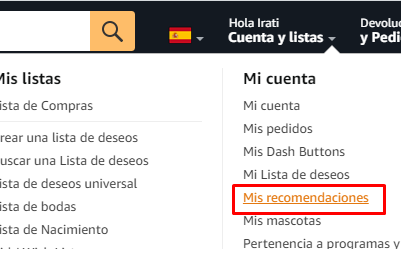
\includegraphics[width=0.45\textwidth]{Figuras/Amazon_acceder_mis_recomendaciones.png}}
    \fbox{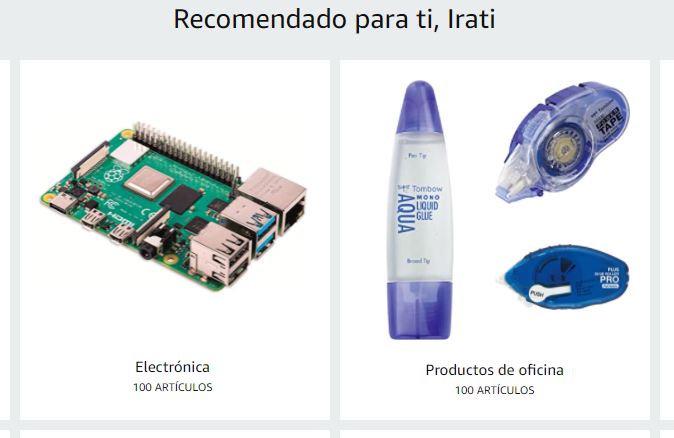
\includegraphics[width=0.45\textwidth]{Figuras/Amazon_recomendaciones.png}}
    \caption{Recomendaciones de Amazon (Fuente: Amazon\autocite{AmazonEsCompra})} 
    \label{fig:AmazonRecomendaciones}
\end{figure}

\subsection{Privacidad digital}
Queda claro que un sistema de recomendación depende plenamente de la información de la que dispone, de forma que, de cuanta más información de los usuarios disponga, más precisión tendrá en sus predicciones. Para obtener esta información muchos anunciantes se han valido de diversas herramientas y utilidades, pero si se ha de destacar alguna, es la utilización de las cookies de terceros. Estas, son definidas por Google\autocite{ComoBorrarHabilitar} cómo:
\\
\begin{minipage}[t]{0.2\linewidth}
\end{minipage}
\hfill
\begin{minipage}[t]{0.9\linewidth}
  \textit{"... son archivos que crean los sitios web que visitas para guardar información de la navegación y facilitar tu experiencia en línea. Gracias a las cookies, los sitios pueden mantener abierta tu sesión, recordar tus preferencias del sitio y proporcionarte contenido relevante en función del lugar donde te encuentres. Hay dos tipos de cookies:
  \begin{itemize}
      \item Las cookies de origen, que las crea el sitio que visitas. El sitio se muestra en la barra de direcciones.
      \item Las cookies de terceros, que las crean otros sitios. Parte del contenido que ves en la página web que visitas, como anuncios o imágenes, pertenece a estos sitios."
  \end{itemize}}
\end{minipage}
\\ \\
A simple vista, estas cookies parecen inofensivas, pero el problema radica en su utilización. Aunque suelen ser usadas con fines analíticos por compañías de marketing online, estas registran el comportamiento de un usuario en la red y crean perfiles de usuarios para ofrecer publicidad personalizada para cada tipo de perfil. Del comportamiento de un usuario en internet se pueden saber sus movimientos, hábitos, páginas que visita, edad, sexo, etc. lo que hace que estos sistemas en ocasiones sean intrusivos y vulneren la privacidad de los navegantes. 
\\ \\
En España y en la Unión Europea existe una legislación sobre la privacidad y la protección de datos en la que se restringen y limitan los datos que estas empresas pueden registrar de la navegación online, el Reglamento General De Protección de Datos (RGPD). En el documento adjunto Anexo \ref{appendix:ProteccionDatos}, sección \ref{appendix:ProteccionDatos_Legislacion} se puede consultar un breve resumen de la legislación en vigor. En lo referente a las cookies, este reglamento presenta varios elementos importantes: 
\begin{itemize}
    \item En primer lugar, debe haber un consentimiento explícito del usuario en el consentimiento de la política de cookies. 
    \item En segundo lugar, la aceptación de las cookies de terceros no ha de ser un impedimento para el uso del servicio.
    \item En último lugar, todas las cookies y rastreadores que operen en la web del propietario deberán ser mostradas al usuario en un lenguaje sencillo.
\end{itemize} 
Aun así, esta legislación no impide que se realice un perfilado del usuario, que se haga un seguimiento de este por la red o que se analice el tiempo que pasa en la página. Con la maduración de la tecnología cada vez más gente se preocupa por el uso que les dan estas empresas a los datos y son más críticos con estas prácticas. Esto ha llegado incluso a la política, donde España está desarrollando una carta pionera de derechos digitales, en la cual, entre otras cosas, recoge el derecho de los usuarios a no ser perfilados (Anexo \ref{appendix:ProteccionDatos}, sección \ref{appendix:ProteccionDatos_Derechos}).
\\ \\
Hoy en día existen muchos navegadores y complementos que permiten bloquear este tipo de rastreadores, lo que ha llevado al sector y a Google a tener que explorar nuevas vías para obtener esta información. La solución propuesta por Google ha sido su nuevo sistema Federated Learning of Cohorts, aprendizaje federado de cortes, con el que se compromete a dejar las cookies de terceros.
\\ \\
Lo que a priori puede significar una buena noticia puede no serlo en realidad. Este sistema permite a Google y a su navegador agrupar y perfilar usuarios en base a sus intereses y perfiles geográficos gracias al historial de navegación y a los datos recogidos durante la navegación. Aunque este sistema no permita que los usuarios puedan ser distinguidos dentro de un grupo, este perfilado supone una persecución y rastreo más grave que el acaecido por las cookies de terceros. En primer lugar, sitúa a Google como principal proveedor de marketing digital, lo que afectaría tanto a la labor de las empresas de marketing digital como al precio que tendrían que pagar estas por la información y los datos.
\\ \\
Ante esta imposición de Google, varias empresas se han pronunciado y han expresado su total desacuerdo con la política, navegadores como DuckDuckGo o Brave la han calificado de anticompetitiva, invasiva y abusiva. Esto se debe a que el navegador de Google, Google Chrome, acapara el 64.19\%\footnote{Fuente: https://gs.statcounter.com/, 27/04/2021} de la red y podría obligar a utilizar su sistema a muchos anunciantes y sitios web.
\\ \\  
\section{Justificación}
Este proyecto es una respuesta al estado de la industria del marketing digital, donde se exprimen al máximo las leyes y normas sobre protección de datos y privacidad digital, y a la actitud de las grandes empresas por perfilar a los usuarios y recoger tanta información de estos como les sea posible.
\\\\
Se quiere demostrar que se puede utilizar el aprendizaje federado preservando la privacidad de los usuarios en un sistema de recomendación, permitiéndoles tener el control total sobre su información desde su propio dispositivo. 
\\ \\
Además, para ello se utilizarán dispositivos como las Raspberries Pi, las cuales servirán para demostrar que no se necesitan dispositivos especialmente potentes para participar en una red de aprendizaje federado, evidenciando que es posible implementar un sistema de recomendación respetuoso con el usuario, acorde al RGPD y salvaguardando los derechos digitales.

% \fancyhead[LE]{}
% \newpage
% \thispagestyle{empty}
% \cleardoublepage

% \chapter{Objetivos y Alcance}
\thispagestyle{fancy}
\fancyhead[LE]{\thechapter.Objetivos y Alcance} 
\section{Objetivos}
Los objetivos de este proyecto pueden clasificarse en varios grupos. Por un lado están los objetivos generales, objetivos que a simple vista no tienen hitos específicos de los que no se puede saber su estado o si se han cumplido o no.
\\ \\
Por otro lado se encuentran los objetivos específicos. Estos, al contrario que los generales, son fácilmente identificables, ya que permiten saber si la tarea se ha completado, y en caso contrario, saber en qué estado se encuentra dicha tarea. Dentro de este grupo se encuentran los objetivos específicos de desarrollo, apartado donde se agrupan los objetivos que permiten saber en qué estado de desarrollo se encuentra el proyecto y qué funcionalidades incorpora. Pero además, también se encuentran los objetivos de estudio, donde se incluyen los objetivos que tienen que ver con el estudio de los diferentes experimentos que se realizarán. 

\subsection{Generales}
El objetivo general de este proyecto es el de desarrollar un sistema de recomendaciones online basado en federated learning. Este sistema se desarrollará sobre otro sistema de recomendaciones ya existente basado en Machine Learning, y se deberá adaptar para su correcto funcionamiento con información descentralizada.
\\ \\
Para respetar la privacidad y derechos de los usuarios, el proyecto deberá incluir la privacidad como patrón de diseño, cumpliendo tanto con las normativas vigentes en Europa y España como con las posibles nuevas medidas que entren en vigor en un futuro. 
\\ \\
Por último, el sistema deberá asegurar que la información se quede en el dispositivo y no se comparta ninguna información que no sea la del propio modelo desarrollado por el participante de la red.
\\ \\
Una vez desarrollado implementado el aprendizaje federado se estudiará la diferencia con el sistema de recomendación centralizado, privacidad, seguridad, eficiencia, etc.

\subsection{Específicos}
Los objetivos específicos son fácilmente reconocibles y concretos, lo que permite saber con exactitud cuándo se han cumplido los objetivos y cuándo no.

\subsubsection{De desarrollo}
Los objetivos de desarrollo tienen que ver con el correcto desarrollo del sistema de recomendación basado en federated learning. 
\\ \\
\textbf{Parametrización y configuración: }
Se tendrán que configurar las plataformas de desarrollo para poder ejecutar el sistema de recomendación centralizado con mayor rapidez y agilizar el desarrollo del proyecto. También se tendrán que configurar las Raspberries y la Jetson Nano, aprovisionarlas del software necesario para ejecutar en ellas el sistema de recomendación y ejecutarlo sin problemas.
\\ \\
\textbf{Desarrollo: }
Se desarrollarán todas las características de los sistemas de recomendación derivadas de la fase de investigación.

\subsubsection{De investigación}
Los objetivos de investigación, al contrario que los de desarrollo, tienen que ver con la búsqueda de soluciones a las incógnitas del proyecto. Es decir, suplir las limitaciones derivadas del federated learning además de la formación del propio alumno en esta tecnología.
\\ \\
\textbf{Formación: }
El alumno deberá formarse en conocimientos sobre Inteligencia Artificial para poder comprender los conceptos. También tendrá que familiarizarse con el código del sistema de recomendación para poder realizar las modificaciones pertinentes en él. Además, el alumno deberá leer artículos científicos sobre federated learning para comenzar a investigar las soluciones a los problemas derivados del proyecto.
\\ \\
\textbf{Sistema de recomendación: }
Se deberá investigar la forma de combinar modelos de IA de cada Raspberry. Además, se investigarán y realizarán las modificaciones pertinentes en el sistema de recomendación para cumplir los siguientes puntos:
\begin{itemize}
    \item Que sea capaz de obtener las recomendaciones para un único usuario en concreto. 
    \item Que sea capaz de guardar y cargar los modelos entrenados de LightFM.
    \item Que el modelo de LightFM sea capaz de admitir aprendizaje incremental.
\end{itemize}

\subsubsection{De estudio}
Los objetivos de estudio tienen que ver con el análisis de los resultados del sistema de recomendación basado en federated learning.
\\ \\
\textbf{Análisis: }
El estudio del sistema tendrá que analizar la diferencia de rendimiento entre el sistema de recomendación con información centralizada y distribuida. También tendrá que analizar cómo afectan los distintos modelos y su combinación al rendimiento del sistema de recomendación.
\\ \\
\textbf{Privacidad: }
Hay que valorar y analizar la privacidad y seguridad de los datos personales de los usuarios tanto en el modelo central, como en el distribuido. Se deberán evitar los problemas de seguridad y privacidad implícitos de la implementación de un sistema de recomendación basado en federated learning

\section{Alcance}
El alcance se centra en concretar qué objetivos entran en el desarrollo del proyecto y cuáles no. Para ello se ha dividido este apartado en dos grupos, los objetivos y tareas que entran en el alcance del proyecto y los que no. La segregación en estos grupos nos permite concretar con más precisión los límites del proyecto, evitando que se amplíe más allá de sus límites. 

\subsection{Dentro del alcance}
Entran dentro del alcance los objetivos y tareas derivadas del desarrollo de un sistema de recomendación basado en federated learning, tanto las tareas de parametrización y configuración del hardware como el desarrollo de software. Esto incluye todos los objetivos específicos de desarrollo mencionados en el apartado anterior.
\\ \\
Del mismo modo quedan dentro del alcance los objetivos de investigación del apartado anterior, ya que son indispensables para el correcto desarrollo del sistema de recomendación
\\ \\
También se incluye el estudio y análisis de los resultados del sistema de recomendación, así como su precisión y sus inconvenientes, es decir, todo lo comentado en los objetivos específicos de estudio.
\\ \\
Para finalizar se incluirá un estudio de la estabilidad legal del sistema en el tiempo. Esto incluye la corroboración del cumplimiento de las actuales medidas de protección de datos y el estudio de las posibles futuras medidas, legislaciones y derechos que limiten el uso de información en Europa.
\\ \\
Se recogera el desarrollo de todo el proyecto en la memoria técnica que será entregada como proyecto fin de grado.

\subsection{Fuera del alcance}
Fuera del alcance queda cualquier estudio de mercado sobre si la solución sería viable económicamente además de cualquier estudio de alternativas a federated learning. 
\\ \\
No se incluirá ni se recogerá ninguna legislación fuera del marco jurídico Español y del Ordenamiento jurídico de la Unión Europea. Lo que deja fuera del alcance cualquier derecho, legislación o restricción de cualquier estado u organización ajeno a los comentados.
\\ \\
Queda fuera del alcance también la encriptación de las comunicaciones entre los diferentes dispositivos.
\\
% \fancyhead[LE]{}
% \newpage
% \thispagestyle{empty}
% \cleardoublepage

\chapter{Consideraciones éticas}
\thispagestyle{fancy}
\fancyhead[LE]{\thechapter.Consideraciones éticas}

En este proyecto se tratan dos consideraciones éticas en mayor medida, la de la defensa del derecho a la privacidad en la era digital y la legalidad para un RS sostenible en el tiempo.

\section{Derecho a la privacidad}

La solución propuesta al problema de agregación de distintas IAs viene de la privacidad como patrón de diseño, motivo y objetivo principal del proyecto. La privacidad digital es un tema controversial a la hora de navegar por internet y en muchas ocasiones, se incumplen derechos fundamentales en el uso de esta red.
\\\\
Tales son las vulneraciones que ocurren, que hay expertos que defienden que no se deben hacer distinciones entre lo digital y lo no digital, ya que vulnerar la privacidad digital es vulnerar el derecho humano de la privacidad. Otros expertos creen que es necesaria una nueva generación de los derechos humanos que incluya los problemas inherentes de vivir en una sociedad digital.
\\\\
En artículos como el “Hacia la cuarta generación de Derechos Humanos: repensando la condición humana en la sociedad tecnológica”\autocite{donasHACIACUARTAGENERACION} del Dr. Javier Bustamante Donas ya se hacía referencia al camino hacia la cuarta generación de los derechos humanos por la tecnologización de la sociedad. En este artículo, el Dr. Javier Bustamante expone varios ejemplos para demostrar la importancia de los derechos digitales. Uno de estos ejemplos es que si se restringe el libre acceso y libre uso de la tecnología se está atentando directamente contra a la libertad de opinión y expresión. Otro claro ejemplo que expresa es el de la censura en China, que es de especial relevancia puesto que afecta a un porcentaje significativo de la sociedad. El caso es que China ha implantado barreras informáticas que impiden la consulta y la visualización de cualquier tipo de páginas web no autorizadas por el gobierno. Además, todo ciudadano chino debe completar un formulario exhaustivo antes de acceder a internet, haciéndolo fácilmente identificable en la red.
\\\\
Con el objetivo de respetar los derechos de los usuarios se tomarán como punto de partida dos declaraciones de derechos digitales con especial relevancia en el contexto de este proyecto, la carta sobre la privacidad digital ded España \autocite{CartaDerechosDigitales} y la declaración de Deusto sobre los Derechos Humanos en Entornos Digitales \autocite{DeclaracionDeustoDerechos}.
\\\\
En cuanto a la declaración de Deusto de los Derechos Humanos en Entornos Digitales, cabe destacar que entre estos derechos los más destacables a cumplir se encuentran los siguientes:
\begin{itemize}
    \item \textit{``Derecho a la transparencia y responsabilidad en el uso de algoritmos''}, ya que toda persona podrá conocer en todo momento como funciona el protocolo de FL y tendrá el control total sobre sus datos.
    \item  \textit{``Derecho a la privacidad en entornos tecnológicos''}, puesto que toda persona al tener el control sobre sus datos puede elegir cuales se usan en la red de FL y de no querer participar puede renegar de ello.
\end{itemize}

España se encuentra redactando una carta sobre la privacidad digital que tendrá un gran impacto en la sociedad y en internet. Supone un hito en Europa y en el mundo que un estado se comprometa a la protección de los derechos digitales de sus ciudadanos (Anexo.\ref{appendix:ProteccionDatos}, \ref{appendix:ProteccionDatos_Derechos} Derechos fundamentales) y como en este trabajo se quieren respetar estos derechos, se ha elaborado el proyecto partiendo del respeto de estos derechos y de la privacidad como patrón de diseño. Debido a que esta carta aún no esta aprobada pero cuando se apruebe será legalmente vinculante se comentará con más detalle en la sección siguiente de legalidad.

\section{Legalidad}
Según el principio de legalidad del código ético y deontológico de la Ingeniería Informática \autocite{CodigoEticoDeontologicoa}, artículo 7, punto 5, todo sistema ha de cumplir tanto con las legislaciones Españolas como Europeas. 
\\\\
Para cumplir con el Reglamento General de Protección de Datos, RGPD (Anexo.\ref{appendix:ProteccionDatos}, \ref{appendix:ProteccionDatos_Legislacion} Legislación ), el propio dispositivo del usuario tiene en su poder el modificar sus datos en caso de que sean inexactos o eliminarlos si desea borrar su huella digital. Por lo cual siempre estará en su mano y bajo su responsabilidad el cómo se utilizan sus datos.
\\\\
Además, con este sistema se pretende cumplir tanto con la legislación vigente como con la pionera carta de derechos digitales de España (Anexo.\ref{appendix:ProteccionDatos}, \ref{appendix:ProteccionDatos_Derechos} Derechos fundamentales) que entrará en vigor en los próximos años. 
\\\\
En esta carta existen dos puntos de gran impacto para este proyecto: los derechos ante la Inteligencia Artificial (Derecho XXIII) y el derecho a no ser localizado y perfilado (Derecho V). Ambos explicados en el apartado Derechos fundamentales \ref{appendix:ProteccionDatos_Derechos} del Anexo.\ref{appendix:ProteccionDatos}.
\begin{itemize}
    \item En cuanto al perfilado de usuarios, es la propia tecnología (FL) la que obliga a su consentimiento, ya que la tecnología parte de la premisa de que los usuarios que participan en la red participan de mutuo acuerdo. Es decir, ningún tipo de red que implemente el FL podrá incumplir esta ley puesto que para entrar en la red hace falta expresarlo explícitamente.
    \item Sobre los derechos ante la IA el usuario tendrá derecho en todo momento a impugnar la recomendación e incluso a corregirla si así lo desea.
\end{itemize}


\fancyhead[LE]{}
\newpage
\thispagestyle{empty}
\cleardoublepage

% \chapter{Metodología}
\thispagestyle{fancy}

\fancyhead[LE]{\thechapter.Metodología} 
La metodología es un factor muy importante de este proyecto, es la hoja de ruta a seguir, y por ello hay que definirla con precisión y saber cuál es la más apropiada.

\section{Consideraciones}
Debido a los objetivos mencionados en el apartado correspondiente anterior, queda claro que existen varios tipos de objetivos en el proyecto. La metodología deberá ayudar a cumplir todos los objetivos específicos para cumplir los objetivos generales. Sin embargo, dentro de los específicos se puede observar que coexisten tres tipos diferentes: de desarrollo, de investigación y de estudio.
\\ \\
Es difícil utilizar una misma metodología para el correcto desarrollo de los tres objetivos, ya que pertenecen a distintas disciplinas, así pues, se ha optado por combinar distintas metodologías para ello. De esta forma se consigue conducir todos los objetivos en una misma dirección. Las metodologías que se combinarán serán:
\begin{itemize}
    \item Metodología Cuantitativa, metodología de investigación.
    \item Modelo espiral, metodología de desarrollo de software.
\end{itemize}

\section{Metodología de Investigación}
La metodología cuantitativa es una metodología de investigación que se centra en la recopilación y el análisis de los datos, lo que nos servirá como guía para los objetivos de estudio y el análisis de los resultados de los experimentos. 
\\ \\
Esta metodología dice que se deben llevar a cabo varias fases de las que solo se realizarán las siguientes tres:
\begin{enumerate}
    \item Definir claramente el problema y lo que se quiere hacer. 
    \item Delimitar el problema, concretar el alcance de la investigación.
    \item Revisión de la literatura, buscar los conocimientos necesarios para realizar el estudio.
\end{enumerate}
Después de haber realizado las tres fases de la metodología de la investigación se aplicará la investigación empírica al estudio, ya que encaja perfectamente con el planteamiento de este proyecto. Esta forma de investigación es una forma de obtener conocimiento a través de la observación o experiencia. Además, mediante este método se nos incita a probar distintos experimentos y modificaciones de estos con el objetivo de encontrar resultados diferentes.\\ \\
Para aplicar esta metodología se usará Ciclo empírico de A.D. de Groot (Fig.\ref{fig:CicloEmpirico}). Este ciclo nos ayuda a ordenar y entender las fases del proyecto, a conocer los siguientes pasos y a no perdernos.
\\ \\
En el primer paso se encuentra la observación. Como el alumno ya ha adquirido la formación en el apartado tres de la metodología cuantitativa podrá empezar observando cómo funciona el sistema de recomendación. A medida que se den más vueltas al modelo, esta observación se realizará sobre los resultados de los experimentos a la hora de aplicar federated learning.
\\ \\
En el segundo paso, el de inducción, se plantean las ideas o hipótesis acerca del paso de observación. En la primera vuelta, estas hipótesis e ideas serán sobre lo que ha aprendido el alumno y sobre cómo se aplicará el federated learning al proyecto. En las demás vueltas serán sobre los resultados observados y cómo estos afectan al proyecto y al estudio y qué mejoras podrían realizarse. 
\\ \\
Tanto la fase de deducción, donde se formulan los experimentos y pruebas a realizar, como la de pruebas, donde se realizan los experimentos para probar las hipótesis y recopilar datos, se sustituirán por la metodología de desarrollo de software en espiral. De esta forma, el modelo del ciclo empírico quedaría combinado con el de espiral para que la investigación y los experimentos que se están realizando mediante software sean concretos y tengan una correcta gestión (véase fig.\ref{fig:MetodologiaCombinada}). 
\\ \\
En el paso de evaluación, se interpretan los resultados de los experimentos de los anteriores dos pasos. En este apartado se hará un gran uso de  la estadística para mostrar la información, tanto gráfica como analiticamente.
\\ \\
Se pueden realizar tantas vueltas al ciclo empírico como sean necesarias.
\begin{figure}[thbp]
    \centering
    \fbox{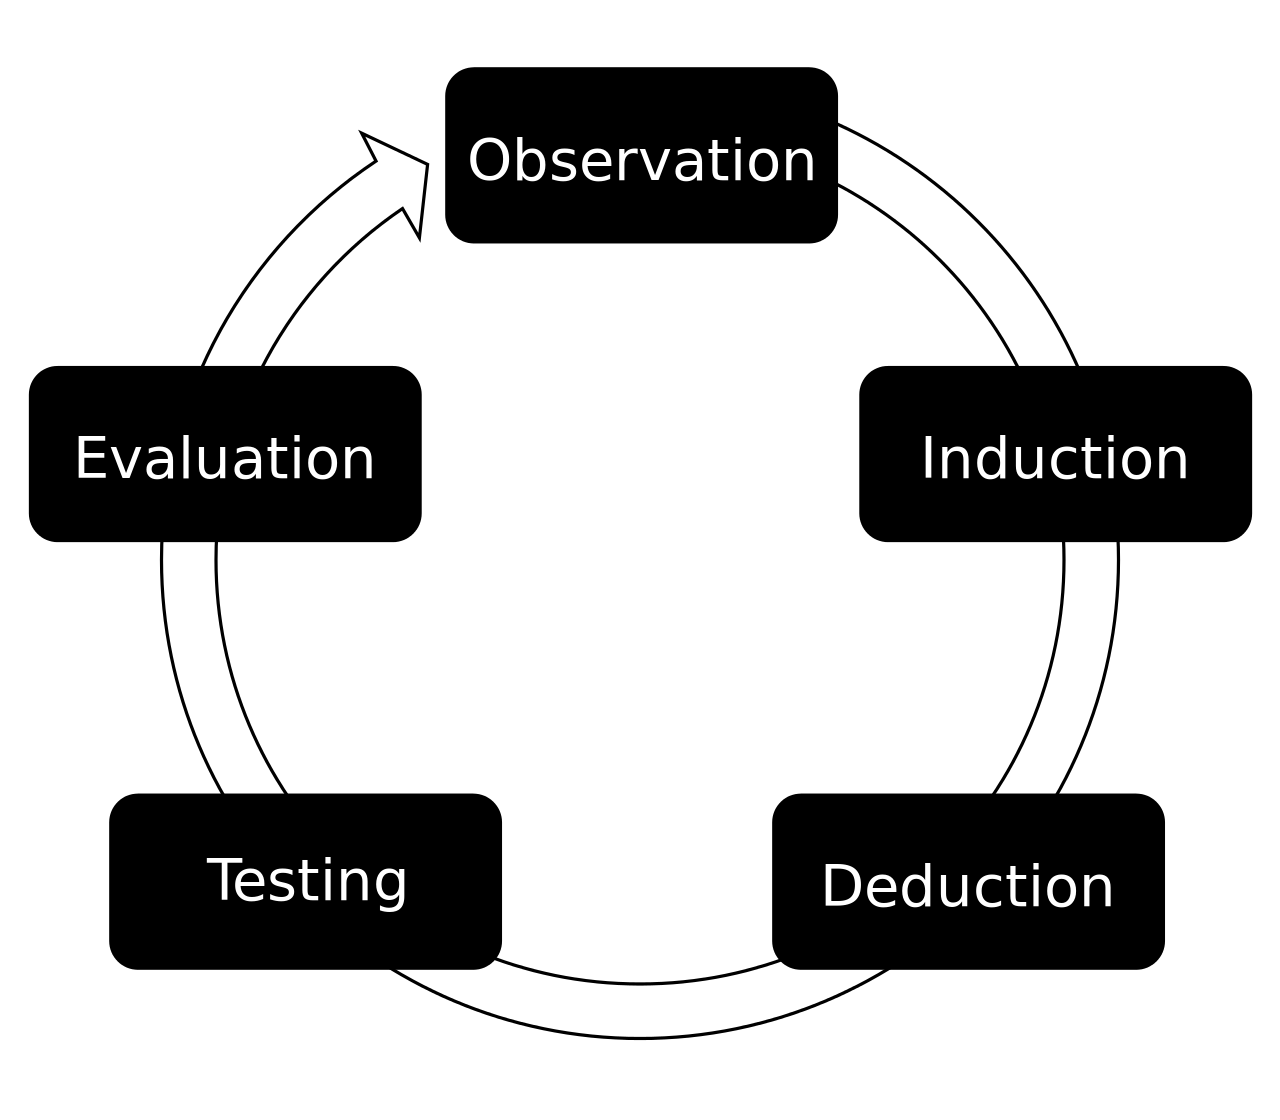
\includegraphics[width=0.45\textwidth]{Figuras/MetodologiaEmpirica.png}}
    \caption{Ciclo empírico de A.D. de Groot (Fuente: Wikipedia\autocite{InvestigacionEmpirica2020})} 
    \label{fig:CicloEmpirico}
\end{figure}
\section{Metodología de desarrollo}

El modelo en espiral (Fig.\ref{fig:MetodologiaEspiral}) formará parte del ya mencionado Ciclo empírico y agrupará los pasos de formulación de los experimentos y su ejecución. Se ha optado por incluir esta metodología dentro de otra para detallar más profundamente cómo será el proceso de desarrollo de software derivado de la investigación realizada.
\\ \\
Se ha elegido este modelo entre otros por varias razones importantes:
\begin{itemize}
    \item Define claramente lo que es un ciclo completo, los pasos a dar y las tareas a realizar. También fija los objetivos al inicio de cada ciclo de la espiral, lo que unido al paso de inducción del ciclo empírico implica que se definen objetivos claros y concisos sobre las hipótesis planteadas.
    \item Al ser un modelo continuo, se pueden realizar tantas iteraciones sobre la espiral como se necesiten, permitiendo desarrollar tantos experimentos como hipótesis se plantean en el apartado de inducción del ciclo empírico. Además, cada vuelta de la espiral incluye el desarrollo de prototipos (lo que en este caso sería un experimento), que al contar con una fase de integración consigue que puedan coexistir todos en el mismo entorno de desarrollo.
    \item Cumple con las fases de Deducción y Testeo del ciclo empírico ya que incluye los pasos de estas en la fase de desarrollo de la espiral.
    \item Por último y más importante, se ha elegido esta metodología porque tiene en cuenta la gestión y análisis de riesgos. Esto tiene gran importancia al tratarse de un proyecto complejo con múltiples dispositivos y tanta cantidad de pruebas a realizar.
\end{itemize}

\begin{figure}[thbp]
    \centering
    \fbox{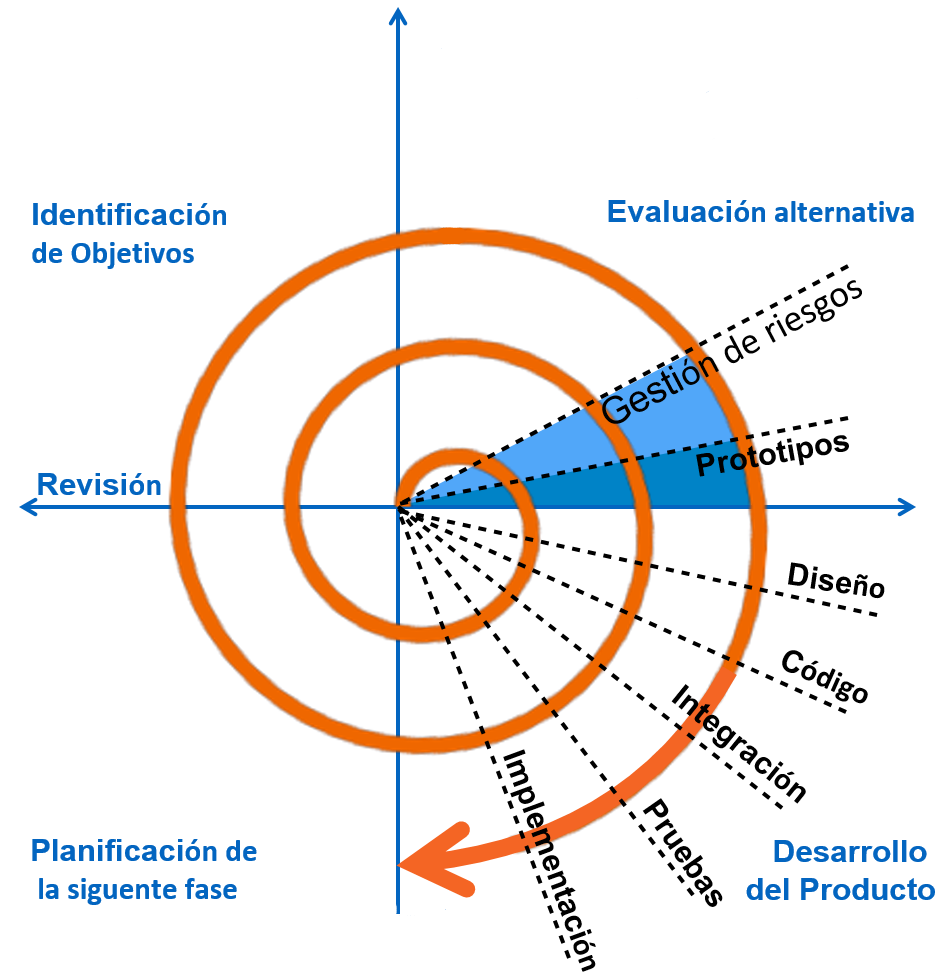
\includegraphics[width=0.6\textwidth]{Figuras/MetodologiaEspiral.png}}
    \caption{Modelo en el Espiral, Autor Desconocido (Fuente: Blog\autocite{CicloVidaSoftware2016})} 
    \label{fig:MetodologiaEspiral}
\end{figure}

\section{Conclusión}
Partiendo del ciclo empírico, escisión de la metodología de investigación cuantitativa, se hará especial incapié en la continua reflexión y teorización sobre el modelo de fededrated learning implantado. 
\\ \\
Para el correcto desarrollo del software, las anteriormente mencionadas fases de deducción y testeo serán incluidas en el modelo de la espiral, consiguiendo así, una gestión eficiente y precisa sobre los pasos a dar tanto en investigación como en el desarrollo de software.
\\ \\
Como se ha comentado anteriormente, la agrupación de estas dos metodologías permitirá combinar la investigación con el desarrollo de software, descubriendo a base de prueba y error y a base de analizar los resultados las mejores soluciones para el sistema de recomendación basado en federated learning.
\\ \\
Por lo cual, una vez el alumno haya definido claramente el problema, su alcance y se haya formado en la tecnología, podrá comenzar a utilizar el ciclo presente en la figura \ref{fig:MetodologiaCombinada}.

\begin{figure}[thbp]
    \centering
    \fbox{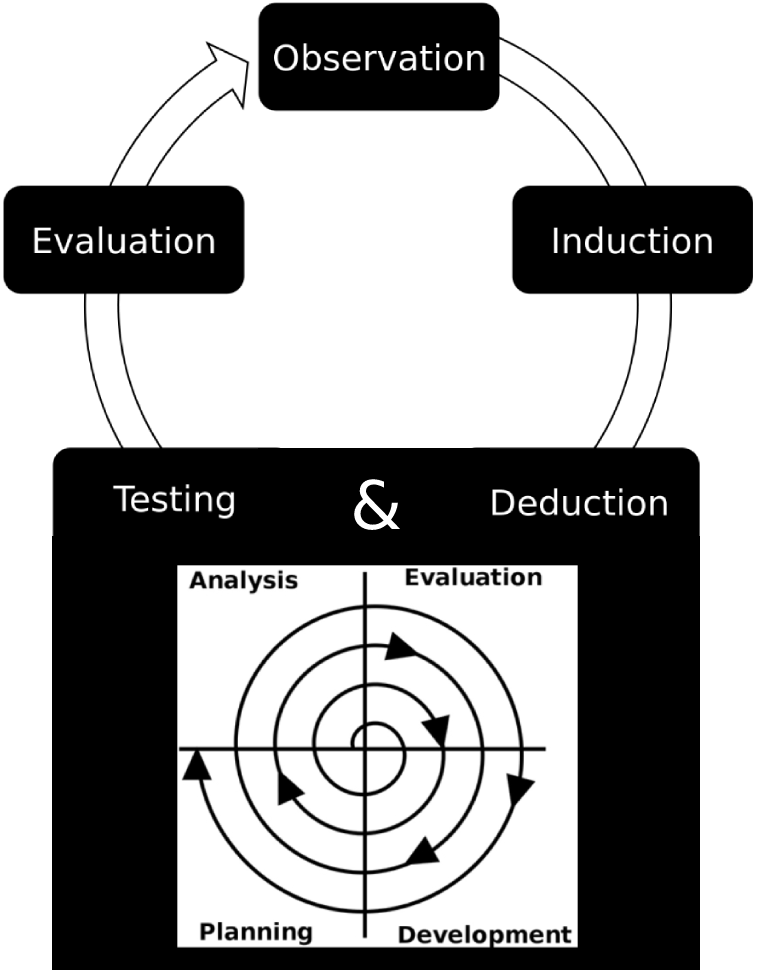
\includegraphics[width=0.6\textwidth]{Figuras/MetodologiaCombinada.png}}
    \caption{Metodología de trabajo del proyecto final de grado (Autor: Ibai Guillén)} 
    \label{fig:MetodologiaCombinada}
\end{figure}
% \fancyhead[LE]{}
% \newpage
% \thispagestyle{plain}
% \cleardoublepage

% \chapter{Planificación}
\thispagestyle{fancy}

\fancyhead[LE]{\thechapter.Planificació} 

La planificación de este proyecto se ha realizado con un diagrama GANTT. Este esta presente en la tabla \ref{table:planificacion}, en caso de querer observar la tabla a una escala mayor esta se encuentra en el Anexo \ref{appendix:Documentos} sección \ref{appendix:Documentos_Planificacion}.
\\ \\
La planificación de este proyecto es un proceso complejo que ha de contener todos los pasos necesarios para conseguir el objetivo del estudio. Para ello se ha dividido en 4 fases de 3 semanas, empezando la primera el 22 de Febrero de 2021 y terminando la ultima fase el 16 de mayo de 2021.
\\ \\
Las tareas de este proyecto se han agrupado en varios grupos:
\begin{itemize}
    \item El registro del proyecto.
    \item La formación.
    \item Configuración del hardware.
    \item Adaptación del RS online a aprendizaje federado.
    \item Desarrollo de la memoria.
    \item Estudio del rendimiento
\end{itemize}
A su vez, estos grupos cuentan con subtareas más concretas que permiten programar adecuadamente la duración del proyecto.
\begin{itemize}
    \item El registro del proyecto. 
        \begin{itemize}
            \item [$\diamond$]Definición de título y descripción.
            \item [$\diamond$]Registro del proyecto a través del formulario.
        \end{itemize}
    \item La formación.
        \begin{itemize}
            \item [$\diamond$]Formación sobre conceptos de Machine Learning.
            \item [$\diamond$]Formación sobre conceptos de los sistemas de recomendación.
            \item [$\diamond$]Formación sobre conceptos de Federated Learning.
            \item [$\diamond$]Formación sobre LightFM.
            \item [$\diamond$]Familiarización con el RS de R.Sánchez.
        \end{itemize}
    \item Configuración del hardware.
        \begin{itemize}
            \item [$\diamond$]Configuración de las RaspBerrys.
            \item [$\diamond$]Configuración de la JetsonNano.
            \item [$\diamond$]Aprovisionamiento de los Sistemas Operativos.
            \item [$\diamond$]Instalar y ejecutar RS.
        \end{itemize}
    \item Adaptación del RS online a aprendizaje federado.
        \begin{itemize}
            \item [$\diamond$]Guardado , cargado y envío de modelos de IA.
            \item [$\diamond$]Agregación de los modelos de IA.
            \item [$\diamond$]Recomendación para un único usuario.
            \item [$\diamond$]Combinar recomendaciones para un único usuario.
            \item [$\diamond$]Combinar recomendaciones para varios usuario.
            \item [$\diamond$]Reentrenar modelos.
            \item [$\diamond$]Visualización de los resultados de rendimiento por gráficas.
        \end{itemize}
    \item Desarrollo de la memoria.
        \begin{itemize}
            \item [$\diamond$]Resumen.
            \item [$\diamond$]Introducción.
            \item [$\diamond$]Antecedentes y Justificación.
            \item [$\diamond$]Objetivos y Alcance.
            \item [$\diamond$]Consideraciones éticas.
            \item [$\diamond$]Metodología.
            \item [$\diamond$]Planificación.
            \item [$\diamond$]Introducción al Federated Learning.
            \item [$\diamond$]Desarrollo.
            \item [$\diamond$]Presupuesto.
            \item [$\diamond$]Conclusiones y Trabajo futuro.
            \item [$\diamond$]Bibliografía.
            \item [$\diamond$]Definiciones y Acrónimos.
            \item [$\diamond$]Anexos.
        \end{itemize}
    \item Estudio del rendimiento.
        \begin{itemize}
            \item [$\diamond$]Estudio del rendimiento de un RS centralizado.
            \item [$\diamond$]Estudio del rendimiento de un RS de modelos agregados.
            \item [$\diamond$]Estudio de rendimiento del sistemas de recomendaciones final.
        \end{itemize}
\end{itemize}
\newpage
\begin{table}
    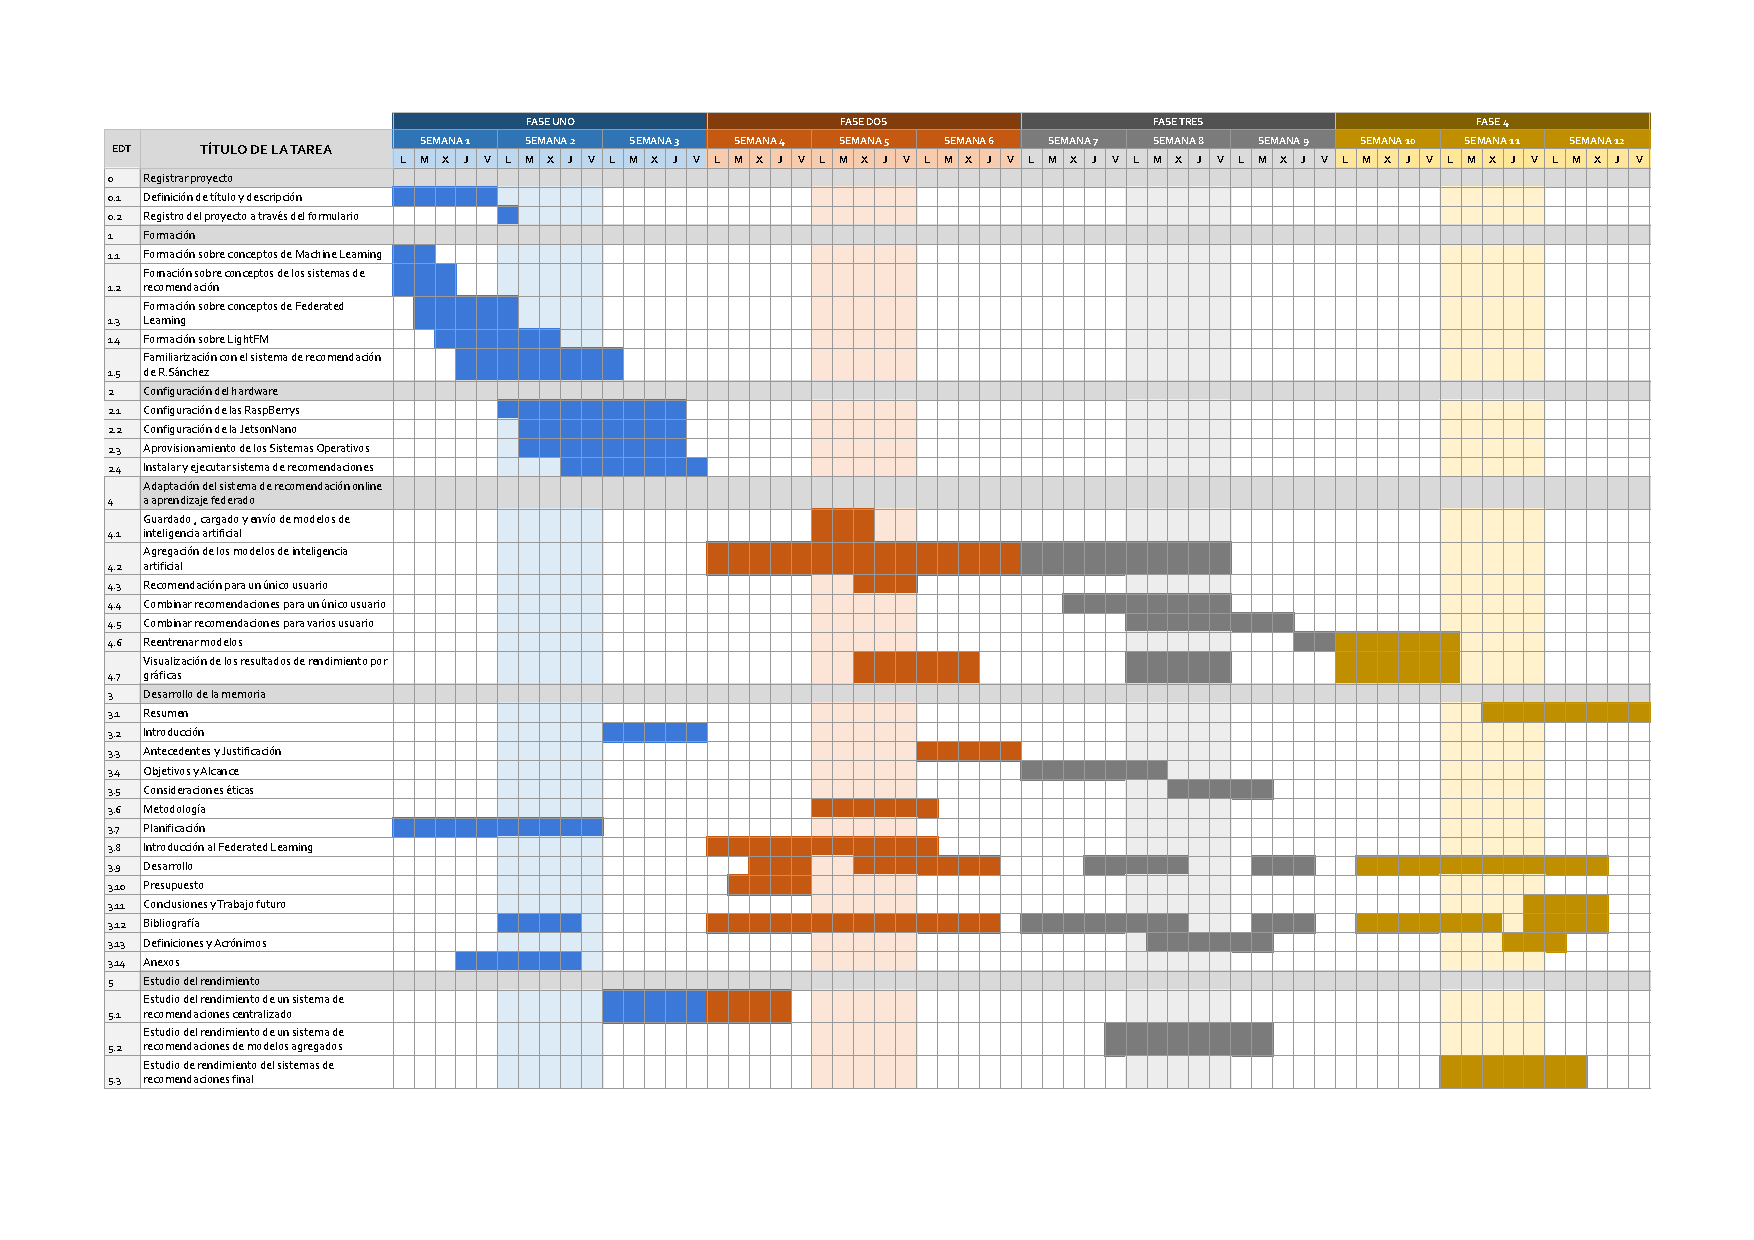
\includegraphics[angle=90,  width=\linewidth, height=\textheight]{PDF/GanttPlanificacion}
    % 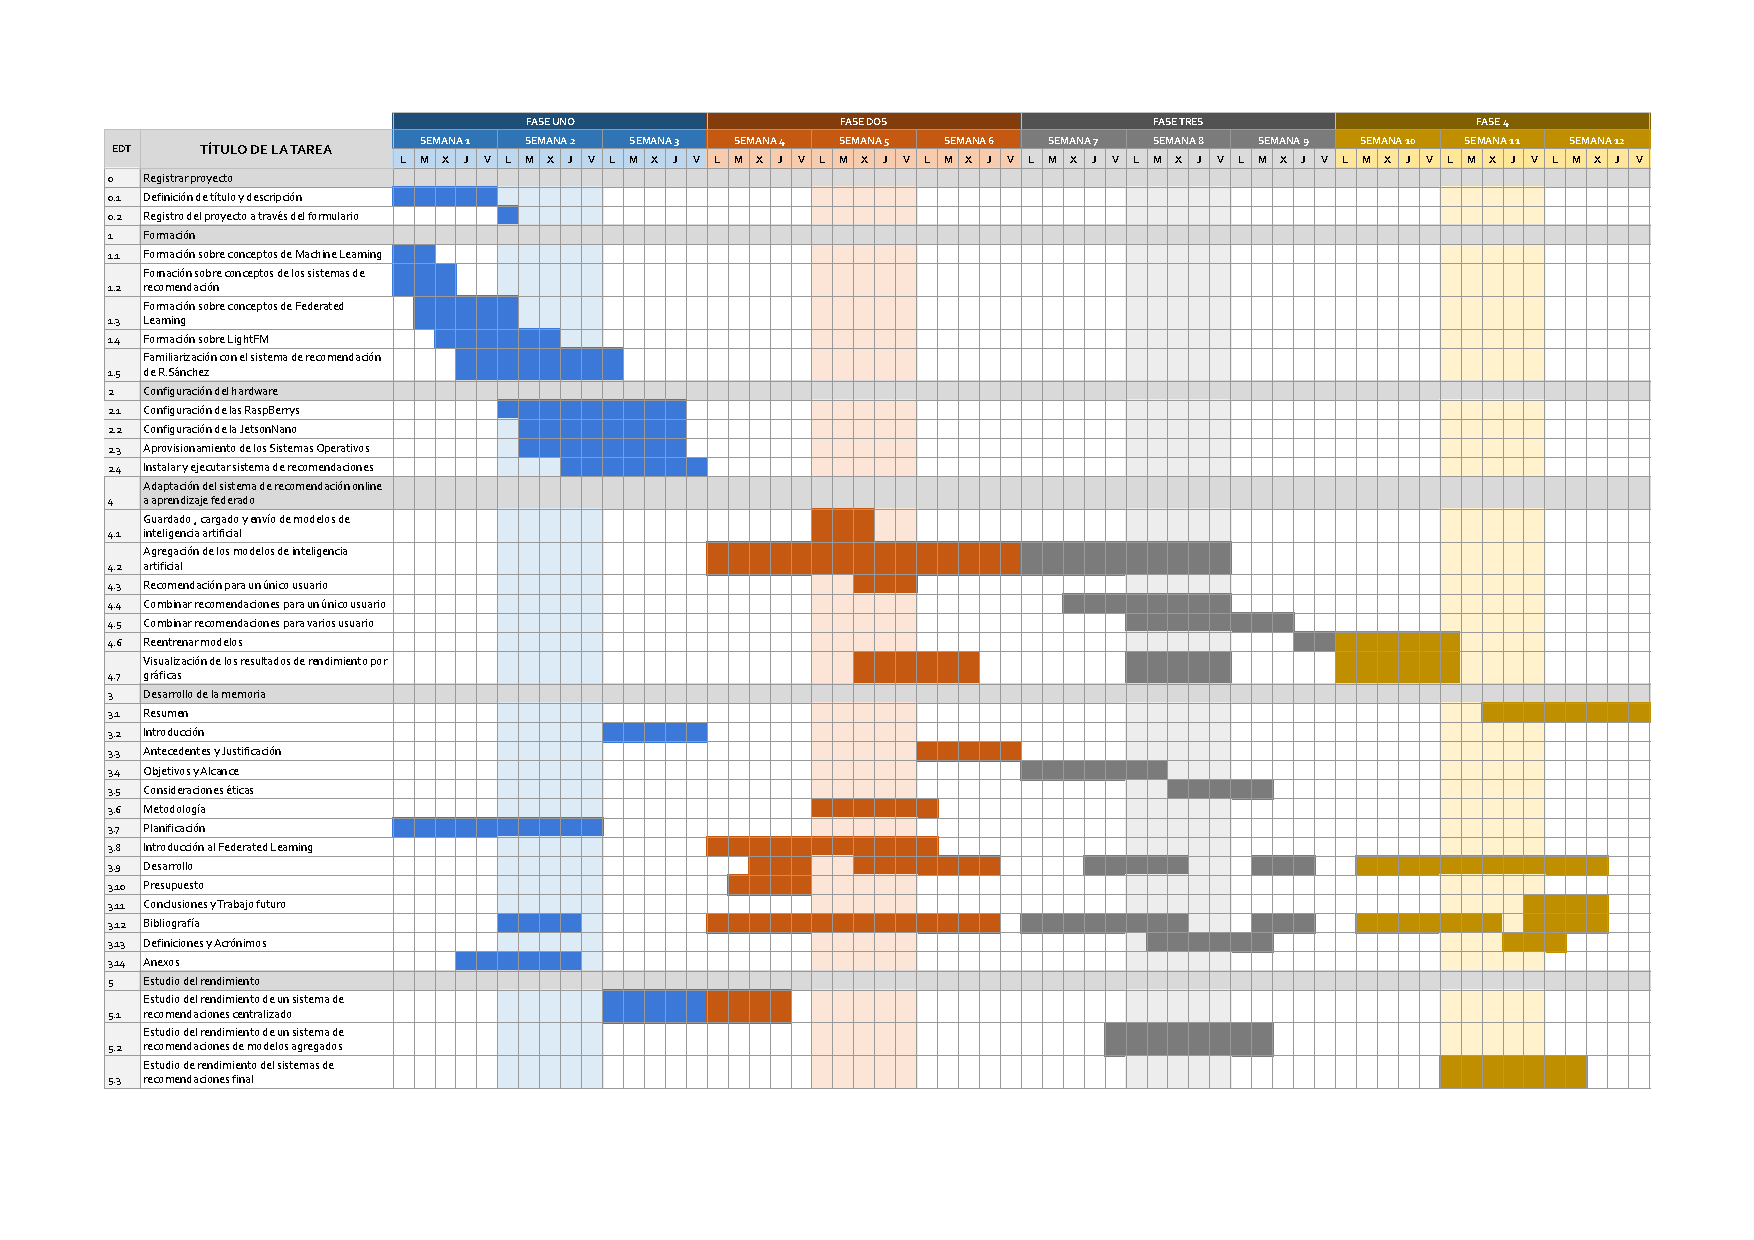
\includepdf[angle=90]{PDF/GanttPlanificacion}
    \caption{Planificación del proyecto}\label{table:planificacion}
\end{table}
% \fancyhead[LE]{}
% \newpage
% \thispagestyle{empty}
% \cleardoublepage

% \chapter{Introducción al Federated Learning}
\thispagestyle{fancy}
\fancyhead[LE]{\thechapter.Introducción al Federated Learning} 
Es de gran importancia comprender y conocer lo que es el Federated Learning (FL) para entender tanto el desarrollo, como la resolución de los problemas y retos que supone su implementación, por eso, en el presente apartado se explicará a conciencia de que se trata esta tecnología. 

\section{Información general}
El FL, es una técnica de ML que entrena un algoritmo a través de diversos dispositivos descentralizados, manteniendo siempre la información en cada uno de ellos (Fig\ref{fig:FedLearArquitectura}). El algoritmo que se busca entrenar en los dispositivos puede ser de cualquier tipo dentro del campo del ML: redes neuronales artificiales, aprendizaje profundo, árbol de decisión, etc. Por lo cual, se puede decir que el FL es una tecnología habilitadora para el entrenamiento de modelos de ML en redes de dispositivos.
\\ \\
Al contrario del ML convencional, que reúne toda la información en un mismo dispositivo, el FL busca entrenar un algoritmo en cada uno de los dispositivos que participen en la red, para luego combinarlos y conseguir un modelo de aprendizaje robusto. Los dispositivos que forman parte de esta red son denominados participantes y todos ellos forman la denominada como red de aprendizaje colaborativo. En esta red, todos aprenden de todos sin necesidad de compartir su información, consiguiendo mejorar la precisión y eficacia del algoritmo. 
\begin{figure}[H]
    \centering
    \fbox{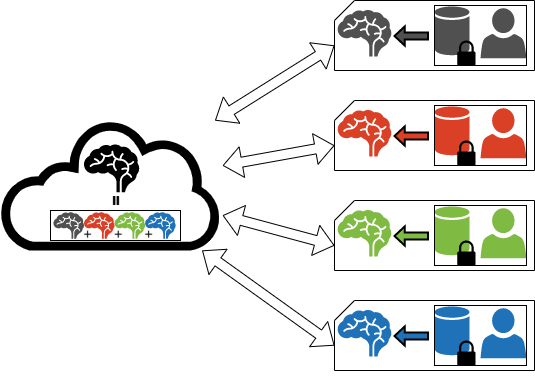
\includegraphics[width=0.5\textwidth]{Figuras/FedLeaConcept.png}}
    \caption{Diagrama de una red de FL} 
    \label{fig:FedLearArquitectura}
\end{figure}
Esta red permite repartir la carga de trabajo entre todos los participantes, puesto que cada uno se encarga de entrenar su propio modelo y enviar al servidor de FL únicamente algunos parámetros del modelo concretos, en ningún momento datos personales ni privados. Esto es posible gracias a que cada vez los dispositivos móviles tienen procesadores más rápidos y más potentes, lo que permite que sean capaces de realizar tareas más complejas y pesadas. De esta forma, se consigue que cada dispositivo sea propietario exclusivo de su información y no tenga que compartirla con ningún otro. Además, hoy en día, los costes de comunicación son superiores a los de computación, por lo que cuanto más acciones se puedan computar en los dispositivos de los participantes menor será el consumo del entrenamiento del algoritmo. 
\\ \\
Sin embargo, debido a estas características propias del FL también sufre de grandes inconvenientes. El hecho de que la red está formada por diferentes participantes la hace heterogénea, con diferentes capacidades de cómputo y diferentes velocidades de conexión entre los distintos participantes, lo que puede incurrir en desconexiones o pérdidas de paquetes durante el proceso de aprendizaje.

\section{Fundamentos y Protocolo}
En general existen dos tipos de entidades en los sistemas de FL, los propietarios de la información (participantes de la red) y el propietario del modelo (servidor de FL). Los propietarios de la información entrenan localmente el modelo con la información de la que disponen, mientras que el propietario del modelo agrega los diferentes parámetros de los modelos recibidos de los participantes para mejorar el algoritmo. 
\\ \\
La comunicación puede ser llevada a cabo de diferentes maneras, de hecho, hay diseños de protocolos de FL como el desarrollado por los autores del trabajo \autocite{bonawitzFederatedLearningScale2019}, que lo dividen en 3 fases:

\begin{itemize}
    \item Selección de los participantes: El servidor elige un grupo de dispositivos conectados para participar en la red.
    \item Configuración: El servidor se configura en base al mecanismo de agregación definido y envía a los participantes el modelo global.
    \item Reporte: El servidor recibe la actualización de cada modelo de su respectivo participante. Más tarde los agrega usando el algoritmo elegido.
\end{itemize}

Además, estos autores definen un parámetro de población con el objetivo de limitar el acceso en caso de que haya muchos participantes, evitando que se conecten a la vez y saturen la red.

\section{Problemas presentes}
\subsection{Técnicos}
Como se ha mencionado antes, implementar el FL implica problemas y costes que hay que asumir y tratar con el objetivo de crear un sistema eficiente y estable. 
\\ \\
Cada actualización del modelo conlleva millones de parámetros, además, se llevan tantas actualizaciones a cabo como precisión se quiera en el modelo. La gran dimensión de las actualizaciones puede incurrir en un aumento de los costes de conexión y generar un cuello de botella, que puede verse agravado por los participantes, ya sea por la asimetría en las velocidades de internet o por la asimetría en la capacidad de cómputo. Es por eso, que para mejorar el rendimiento y reducir el coste de comunicación se deben considerar varias cosas.
\begin{itemize}
    \item En primer lugar, todos los dispositivos deben contar con una conexión estable, preferiblemente conexión por cable, o en su defecto conexión inalámbrica por Wi-Fi, descartando en lo posible todas aquellas conexiones por telefonía móvil.
    \item En segundo lugar, para minimizar el número de rondas de comunicación se puede realizar computación adicional en los dispositivos para que la agregación global se realice antes.
    \item También se puede reducir el tamaño de las comunicaciones, ya sea por compresión del modelo, compresión de los datos, o por el uso de una pequeña muestra representativa de estos en vez de enviarlos por completo.
    \item Por último, se pueden minimizar las actualizaciones de los modelos en base a la importancia de estas. Evitando enviar el modelo global hasta que este no suponga una clara mejora para los participantes.
\end{itemize}

\subsection{Privacidad}
Uno de los objetivos principales del FL es la protección de la privacidad de los usuarios. Los usuarios solo necesitan compartir los parámetros del modelo de ML, en lugar de compartir los datos reales. No obstante, varios estudios han demostrado que estos modelos aún pueden ser susceptibles a ataques informáticos que puedan extraer datos reales.
\\ \\
Véase un ejemplo de vulnerabilidad con FaceScrub, un dataset con más de cien mil imágenes de caras de 530 personas. Mientras se desarrollaba el modelo ML, los desarrolladores se percataron de que, tan solo con inspeccionar el modelo ML, los atacantes podían extraer el 90\% de la información real.
\\ \\
Por mucho que se haya avanzado en el desarrollo de modelos que protejan a los usuarios contra posibles ataques informáticos, esta susceptibilidad a exploits aun sigue patente. Con tan solo acceder al modelo ML de un sistema de reconocimiento por voz, es posible lograr extraer datos como la etnia o género de los usuarios \autocite{melis2018exploiting}. 
\\ \\
En un artículo publicado por expertos en ciberseguridad, se especifica otro caso en el que, mediante ataques relativamente sencillos contra plataformas de la talla de Amazon Machine Learning, es posible extraer modelos basados en árboles de decisión o en regresión logística \autocite{tramèr2016stealing}.

\subsection{Seguridad}
Los modelos de datos de FL son también susceptibles a ataques de envenenamiento de datos. Un participante puede ir entrenando datos y enviándolos al servidor para su posterior procesamiento y análisis. Sin embargo, otro participante puede crear una serie de datos corruptos y enviarlos al servidor con el fin de generar falsos parámetros. Este tipo de ataques, con la desclasificación de los procesos Deep Learning como principal objetivo, tienen una posibilidad de éxito del 90\% si se ejecutan bien \autocite{armknechtGuideFullyHomomorphic2015}.
\\ \\
A diferencia de los ataques de envenenamiento de datos, cuyo objetivo es la generación de datos corruptos para alterar el resultado del modelo generado, los ataques de envenenamiento por modelo buscan alterar el modelo generado en su totalidad. Cuando el modelo de datos generado a través de FL es muy grande y cuenta con una gran cantidad de participantes, este tipo de ataque tiende a ser más exitoso \autocite{bhagoji2019analyzing}.
\\ \\
Existen maneras de prevenir este ataque, como por ejemplo, analizando si el modelo generado por un participante puede ayudar a mejorar el modelo global de datos. Si se da el caso de que no, este modelo será marcado como potencialmente peligroso, y se analizarán los cambios realizados en el modelo de manera exhaustiva para comprobar si se trata de un atacante. 
\\ \\ 
Otra solución parecida consiste en recorrer el servidor y ver si un modelo es muy diferente del resto de modelos. Si es muy diferente, se realiza un análisis de este para comprobar de primera mano si se trata de un atacante.
% \fancyhead[LE]{}
% \newpage
% \thispagestyle{empty}
% \cleardoublepage

% \chapter{Desarrollo}
\thispagestyle{fancy}
\fancyhead[LE]{\thechapter.Desarrollo}
% \newpage


% \section{Requisitos del sistema}
Como bien se ha mencionado previamente, este proyecto trata de adaptar el sistema de recomendación realizado por R.Sánchez \autocite{sanchez-corcueraPersuasionbasedRecommenderSystem2020} a un sistema de recomendación basado en Federated Learning que permita el aprendizaje colaborativo de los participantes. Es por ello que para conocer los requisitos iniciales de diseño del sistema de recomendación se remite al trabajo del autor.
\\ \\
En este apartado se presentarán únicamente los requisitos de la adaptación del sistema y se partirá del trabajo realizado por R.Sánchez. Se presentarán dos tipos de requisitos. En primer lugar los requisitos no funcionales de diseño, las condiciones que debe cumplir la especificación del diseño para cumplir los objetivos del proyecto. En segundo lugar, los requisitos funcionales, las condiciones que ha de cumplir el sistema para ser capaz de funcionar sobre el hardware del que se dispone.

\subsection{No Funcionales}
En cuanto a los requisitos no funcionales se encuentran todos aquellos que se han tenido en cuenta a la hora de plantear el diseño del sistema, es decir, todos los inherentes de la privacidad como patrón de diseño. Por ello el sistema :
\begin{itemize}
    \item [\textbf{RNF1}] Mantendrá toda información de los usuarios en sus dispositivos.
    \item [\textbf{RNF2}] No expondrá la información de los modelos de inteligencia de los usuarios a otros usuarios.
    \item [\textbf{RNF3}] No discriminará entre los modelos de inteligencia artificial a la hora de tomar decisiones.
    \item [\textbf{RNF4}] No perjudicará deliberadamente al modelo de un participante.
    \item [\textbf{RNF5}] No compartirá información que no sea sintética.
    \item [\textbf{RNF6}] No extraerá información de los modelos de los participantes.
    \item [\textbf{RNF7}] Combinará los diferentes modelos de los participantes sin acceder a su información.
    \item [\textbf{RNF8}] Cumplirá tanto con la LOPD-GDD como con el RGPD (véase Apéndice\ref{appendix:ProteccionDatos}, sección \ref{appendix:ProteccionDatos_Legislacion}).
    \item [\textbf{RNF9}] Respetar los derechos digitales de los usuarios y cumplir con la carta de derechos digitales de España (véase Apéndice\ref{appendix:ProteccionDatos}, sección \ref{appendix:ProteccionDatos_Derechos}).
\end{itemize}
\subsection{Funcionales}
Los requisitos funcionales son básicos en este proyecto para que el sistema sea compatible y ejecutable en el hardware. Por ello, para que el sistema sea compatible con el harware se han definido los siguientes requisitos:
\begin{itemize}
    \item [\textbf{RF1}] El sistema ha de ser ejecutable bajo la arquitectura ARMv8.
    \item [\textbf{RF2}] El sistema ha de ser ejecutable bajo la arquitectura x86 y x64.
    \item [\textbf{RF3}] El sistema ha de ser ejecutable bajo la arquitectura AArch64.
    \item [\textbf{RF4}] El sistema ha de ser ejecutable en Linux.
    \item [\textbf{RF5}] El sistema ha de ser ejecutable en Windows.
\end{itemize}

Además, al margen de los requisitos de compatibilidad también se encuentran los requisitos de recursos, y es que teniendo un hardware poco potente es imprescindible que el software sea lo más óptimo posible para aprovecharlo al máximo. Es por eso que también se definen los siguientes requisitos:
\begin{itemize}
    \item [\textbf{RF6}] El sistema ha de ser capaz de entrenar los modelos en un espacio de tiempo razonable, siendo este siempre inferior a los 100 segundos por cada 10 epochs.
    \item [\textbf{RF7}] El sistema de recomendación no puede colapsar el dispositivo que lo ejecute,
    \item [\textbf{RF8}] El sistema de recomendación debe permitir que el dispositivo pueda funcionar con normalidad durante su ejecución.
\end{itemize}
% \newpage
% \section{Gestión de riesgos}\label{GestionRiesgos}
El motivo de esta sección viene de la definición del modelo en espiral como metodología clave para el desarrollo de este proyecto. Este modelo recoge la identificación y gestión de riesgos como pieza fundamental del ciclo de vida, y en un proyecto con tal complejidad técnica y con tantos dispositivos involucrados, es indispensable tener un plan de acción ante cualquier incidente.
\\ \\
Con tantos dispositivos que gestionar, el proceso de configuración de estos puede llegar a ser algo pesado, y más si alguno de estos falla o se rompe. Si se rompiese o se corrompiese una tarjeta SD de una Raspberry Pi habría que reinstalar y configurar todos los paquetes a mano, proceso que puede ser bastante largo puesto que requiere de interacción humana. Para evitar esto se ha tomado la decisión de crear un script de aprovisionamiento tanto para la Nvidia Jetson Nano como para las Raspberries Pi, de esta manera, en caso de que una tarjeta SD se averiase, bastaría con cambiarla, configurar el protocolo SSH para acceder remotamente a ella y ejecutar el script. Cuando el proceso terminase el dispositivo estaría listo para poder ejecutar el proyecto sin ningún problema.
\\ \\
Las tareas de IA no son especialmente livianas para un dispositivo, lo que durante un entrenamiento prolongado en el tiempo podría incurrir en un aumento de temperatura de este. Para evitar que los dispositivos alcancen temperaturas elevadas o que sufran cualquier tipo de cortocircuito por su manipulación inadecuada se ha optado por instalarlos en un rack (Fig \ref{fig:RackRaspberry}). Esta carcasa aparte de proteger los dispositivos viene equipada con ventiladores que ayudarán a que la temperatura de estos sea siempre la adecuada.

\begin{figure}[thbp]
    \centering
    \fbox{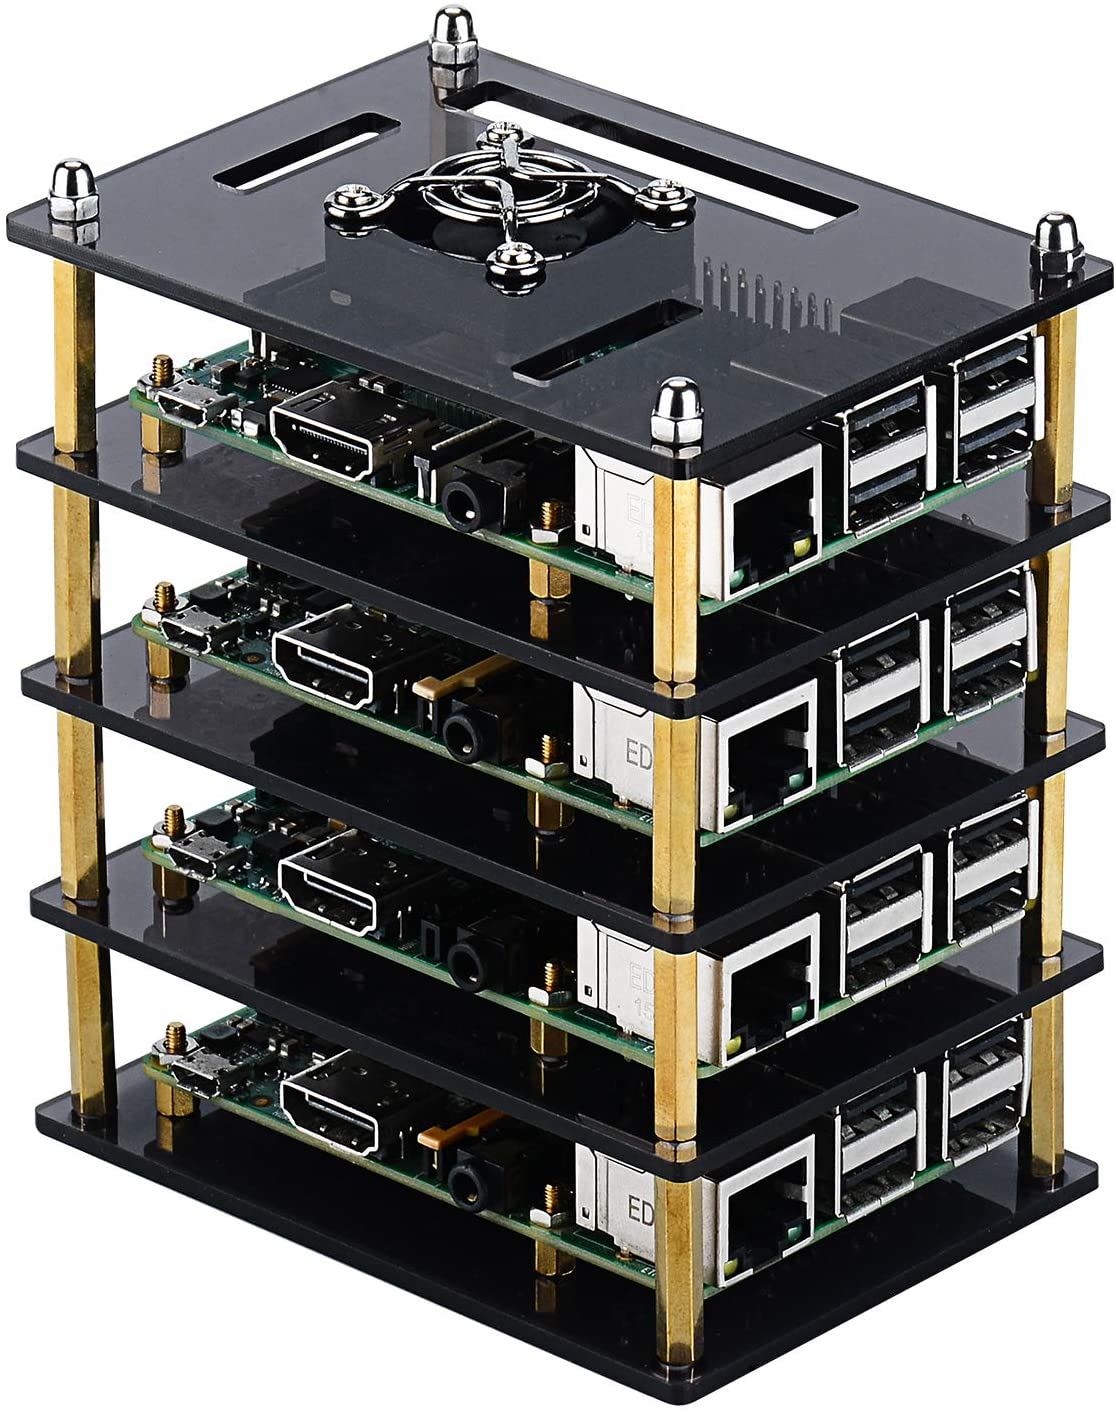
\includegraphics[width=0.3\textwidth]{Figuras/RaspBerryRack.jpg}}
    \caption{Rack para Raspberry Pi (Fuente: Amazon\autocite{ParaRaspberryPi})}
    \label{fig:RackRaspberry}
\end{figure}

Durante el desarrollo se tiene que acceder a estos dispositivos en multitud de ocasiones, para ello se utiliza el protocolo SSH. Sin embargo, al realizarse este proyecto en un ámbito doméstico, existe la probabilidad de que el router sea reiniciado o apagado por cualquier causa externa al proyecto. En tal caso puede que las direcciones IP sean sustituidas y haya que realizar un análisis de la red o acceder físicamente a estos dispositivos para averiguar la IP. Para evitar este proceso se ha instalado el paquete \textit{AVAHI}\footnote{AVAHI es un servicio que facilita el descubrimiento de dispositivos en la red local a través de mDNS/DNS-SD.}, que permite acceder mediante SSH a las Raspberries sustituyendo la dirección IP por el nombre de servidor de los dispositivos.
\\ \\
Para gestionar los cambios que se irán haciendo sobre el software sin problemas, es indispensable contar con herramientas de control de versiones. Estas herramientas permiten gestionar cuándo se han realizado qué cambios y en caso de necesitar una versión anterior, se podrían revertir los cambios con facilidad. En este caso, tanto para el desarrollo del proyecto como para el desarrollo de la memoria se utilizará Git como controlador de versiones. Además, se utilizará Github como repositorio de código en la nube, para así poder clonar el repositorio a los dispositivos fácilmente.

% \newpage
% \section{Especificación del diseño}
Teniendo en cuenta los anteriores requisitos y los objetivos del proyecto, la especificación del diseño concretará cómo se han diseñado las diferentes funcionalidades y cómo se ha implementado el FL en el proyecto. Para ello, se dividirá el capítulo en las siguientes secciones: 

\begin{enumerate}
    \item \textbf{Arquitectura}, tanto la configuración de los dispositivos como el cómo se interconectan y comunican entre sí.  
    \item \textbf{Datos involucrados}, los datos que intervienen en el proyecto. 
    \item \textbf{Protocolo de Federated Learning}, los pasos a llevar a cabo por el RS basado en FL.
    \item \textbf{Securización de las comunicaciones}, la forma en la que se van a llevar a cabo las comunicaciones,
    \item \textbf{Agregación de los modelos}, cómo se van a agregar los modelos de los distintos participantes.
    \item \textbf{Valoración de las predicciones}, explicación de la métrica que se utilizará para valorar la precisión de los rankings predichos.
\end{enumerate}

\newpage
\subsection{Arquitectura}
En este apartado se explicarán los componentes que forman parte de la arquitectura de la solución, el cómo se deben conectar para emular una red de FL y el propio montaje físico de los dispositivos. De esta forma, se podrá comprender por qué se han seleccionado los dispositivos que van a participar en el FL, cuál es el mapa de red de una red de FL, cómo se va a representar localmente y cómo queda el montaje de todos los dispositivos acorde al mapa de red.  

\subsubsection{Componentes}
Para la recreación de un ejemplo real de una red de FL se han utilizado dispositivos de capacidad de cómputo acotada como son las Raspberries Pi. De esta forma, se pretende demostrar la viabilidad de la aplicación del FL a campos como el del internet de las cosas, donde los dispositivos participantes disponen de escasa capacidad de cómputo.
\\ \\
De la misma forma, con el objetivo de demostrar que no se necesita un supercomputador para realizar una agregación de modelos, se ha utilizado la NVIDIA Jetson Nano como núcleo central para ello.
\\ \\
Los dispositivos que se utilizarán en concreto son los siguientes: (x4) Raspberry Pi 3 B+ (Fig. \ref{fig:RaspBerrryBPlus}), (x1) NVIDIA Jetson Nano 2GB (Fig. \ref{fig:JetsonNano2GB}) y (x1) Genius switch (Fig. \ref{fig:Switch}).

\begin{figure}[H]
    \begin{minipage}[t]{0.49\linewidth}  % <---
        \centering
        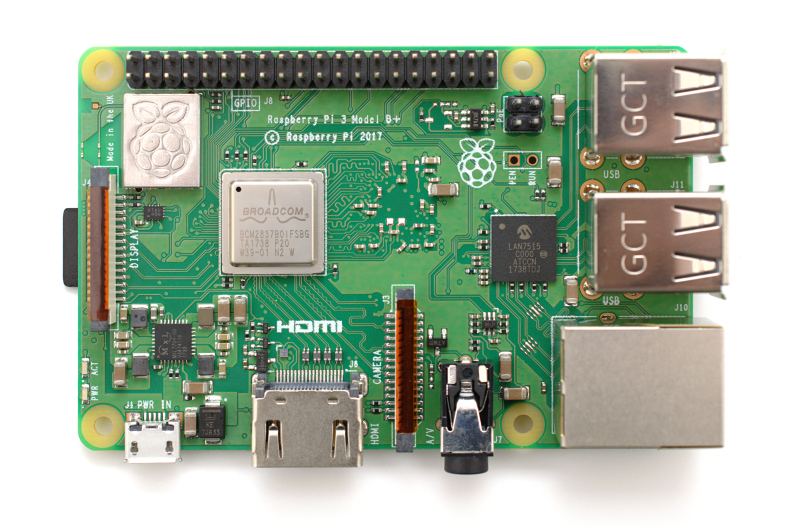
\includegraphics[height=0.1\textheight]{Figuras/Raspberry_Pi_3_B+.png}
        \caption{Raspberry Pi 3 B+ \\ (Fuente: Wikipedia\autocite{ArchivoRaspberryPi})} 
        \label{fig:RaspBerrryBPlus}
    \end{minipage}
    \hfill
    \begin{minipage}[t]{0.5\linewidth}  % <---
        \centering
        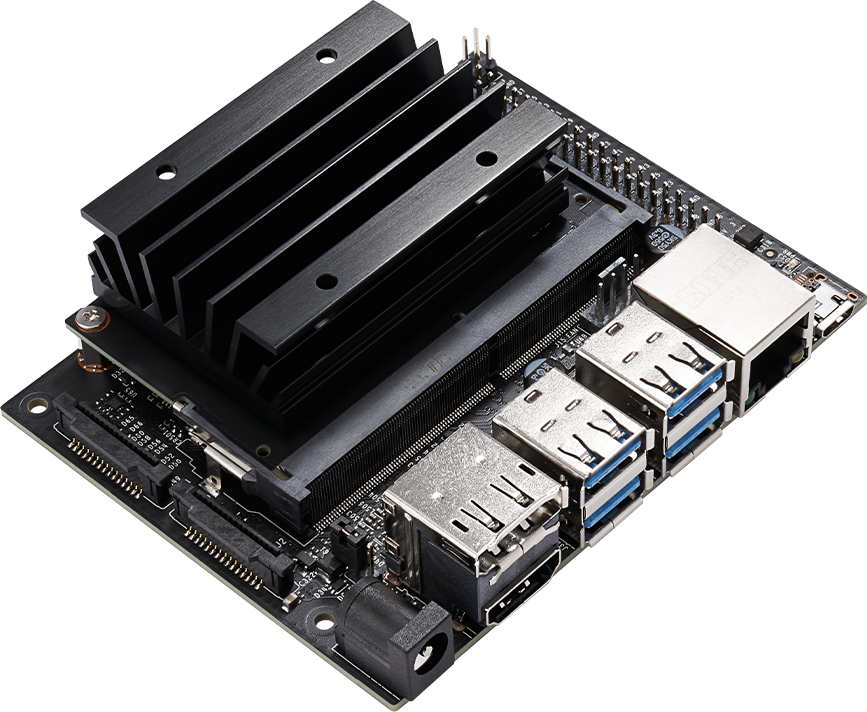
\includegraphics[height=0.1\textheight]{Figuras/nvidia_jetson_nano_2GB.png}    
        \caption{NVIDIA Jetson Nano 2GB \\ (Fuente: NVIDIA\autocite{JetsonNano})} 
        \label{fig:JetsonNano2GB}
    \end{minipage}
\end{figure}
\begin{figure}[H]
    \centering
    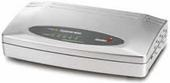
\includegraphics[height=0.1\textheight]{Figuras/genius_switch.jpg}    
    \caption{Switch Genius} 
    \label{fig:Switch}
\end{figure}
\newpage

\subsubsection{Mapa de red}
Las conexiones entre los dispositivos que interactúan en la red (Raspberries y Jetson Nano) será por cable, conectando todos al mismo switch para permitir la comunicación entre ellos. A su vez, este switch se conectará al router que provee de acceso a internet, permitiendo así, que los ordenadores de la red puedan acceder a estos dispositivos y estos dispositivos puedan conectarse a internet para lo que necesiten. Todo ello queda representado en el mapa de la figura \ref{fig:MapaRed}, que sería el mapa de red físico del que parte el proyecto.
\begin{figure}[H]
    \centering
    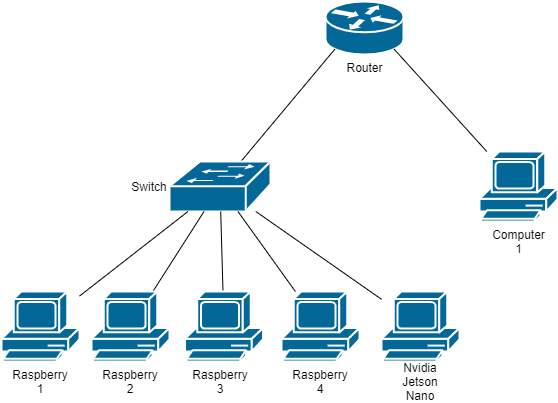
\includegraphics[width=\textwidth]{Figuras/Network_map.png}    
    \caption{Mapa de red física} 
    \label{fig:MapaRed}
\end{figure}

Esta arquitectura de red lo que permite es que desde el ordenador 1 se pueda acceder a cualquier dispositivo mediante ssh para su configuración y ejecución de experimentos. A su vez, estos dispositivos permanecen físicamente separados los unos de los otros mientras mantienen acceso a internet para realizar tareas de descarga de paquetes, actualizaciones, envío de datos, etc. En este caso, para la transferencia de archivos y ficheros se utilizará el protocolo SCP, ya que no entra dentro del alcance el desarrollo de ningún sistema de comunicación y el protocolo SCP es fácilmente combinable con el protocolo ssh.

\pagebreak

Sin embargo, desde el punto de vista de la red de FL que se quiere simular, el mapa de red incluiría los siguientes cambios:
\begin{itemize}
    \item Cada participante tendría su propia red de área local.
    \item La conexión al servidor de agregación se haría a través de internet.
    \item Los participantes no tendrían ninguna conexión ni relación entre sí.
\end{itemize}
De este modo, el mapa de la red de FL representado en el proyecto quedaría acorde a la figura \ref{fig:FLMapaRed}, aunque el mapa de red sobre el que se opere físicamente sea el de la figura \ref{fig:MapaRed}.

\begin{figure}[H]
    \centering
    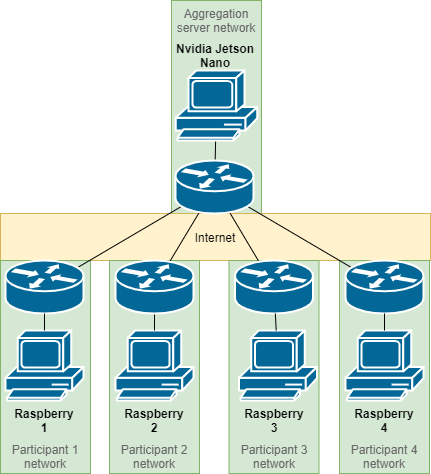
\includegraphics[width=0.8\textwidth]{Figuras/FL_network_map.png}    
    \caption{Mapa de la red de FL} 
    \label{fig:FLMapaRed}
\end{figure}

\pagebreak

\subsubsection{Montaje físico}
Una vez realizados todos los mapas y diagramas para la configuración de la red, se procedió a conectar los dispositivos acorde al mapa de red físico (fig. \ref{fig:MapaRed}). Para este montaje, se acoplaron las Raspberries que representan a los participantes en el rack mencionado en la sección de gestión de riesgos \ref{GestionRiesgos} de este mismo capítulo. Después de conectar todos los cables el montaje quedó como se puede ver en las siguientes imágenes.
\begin{figure}[H]
    \centering
    \begin{minipage}[t]{0.49\linewidth}  % <---
        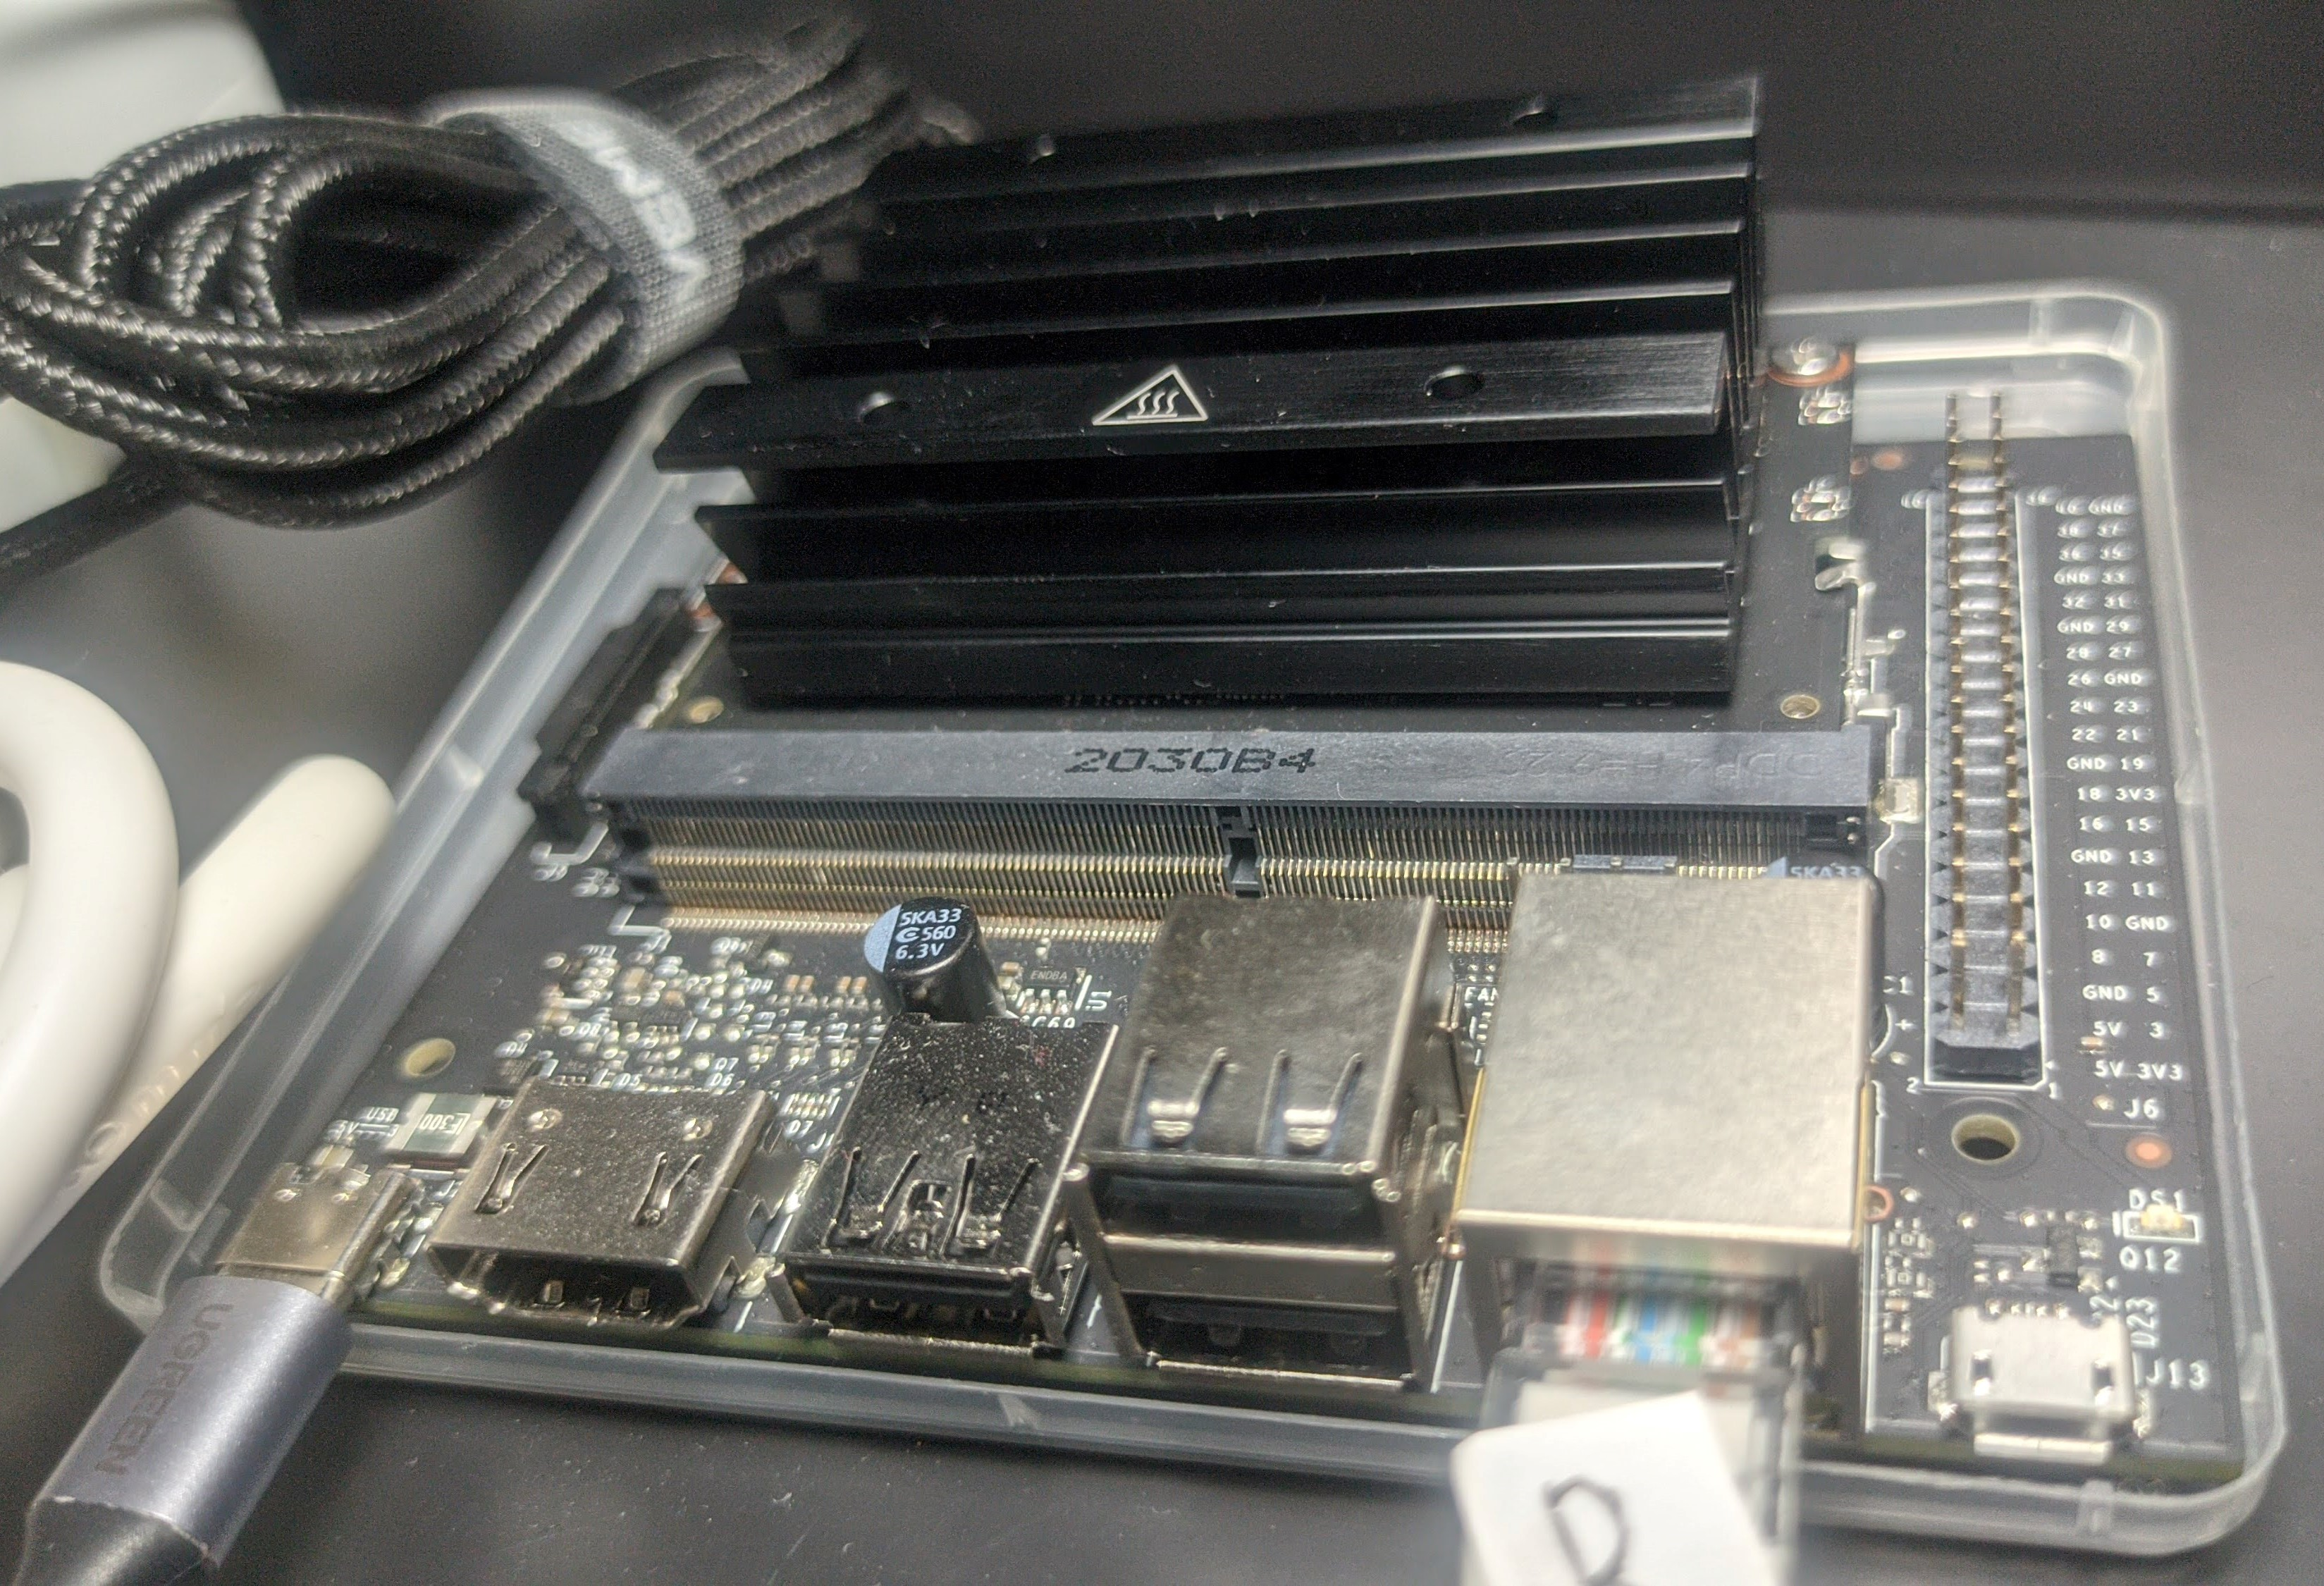
\includegraphics[height=0.2\textheight]{Figuras/jetsonnano.jpg}
        \caption{Montaje de la Jetson Nano} 
    \end{minipage}
    \hfill
    \begin{minipage}[t]{0.5\linewidth}  % <---
        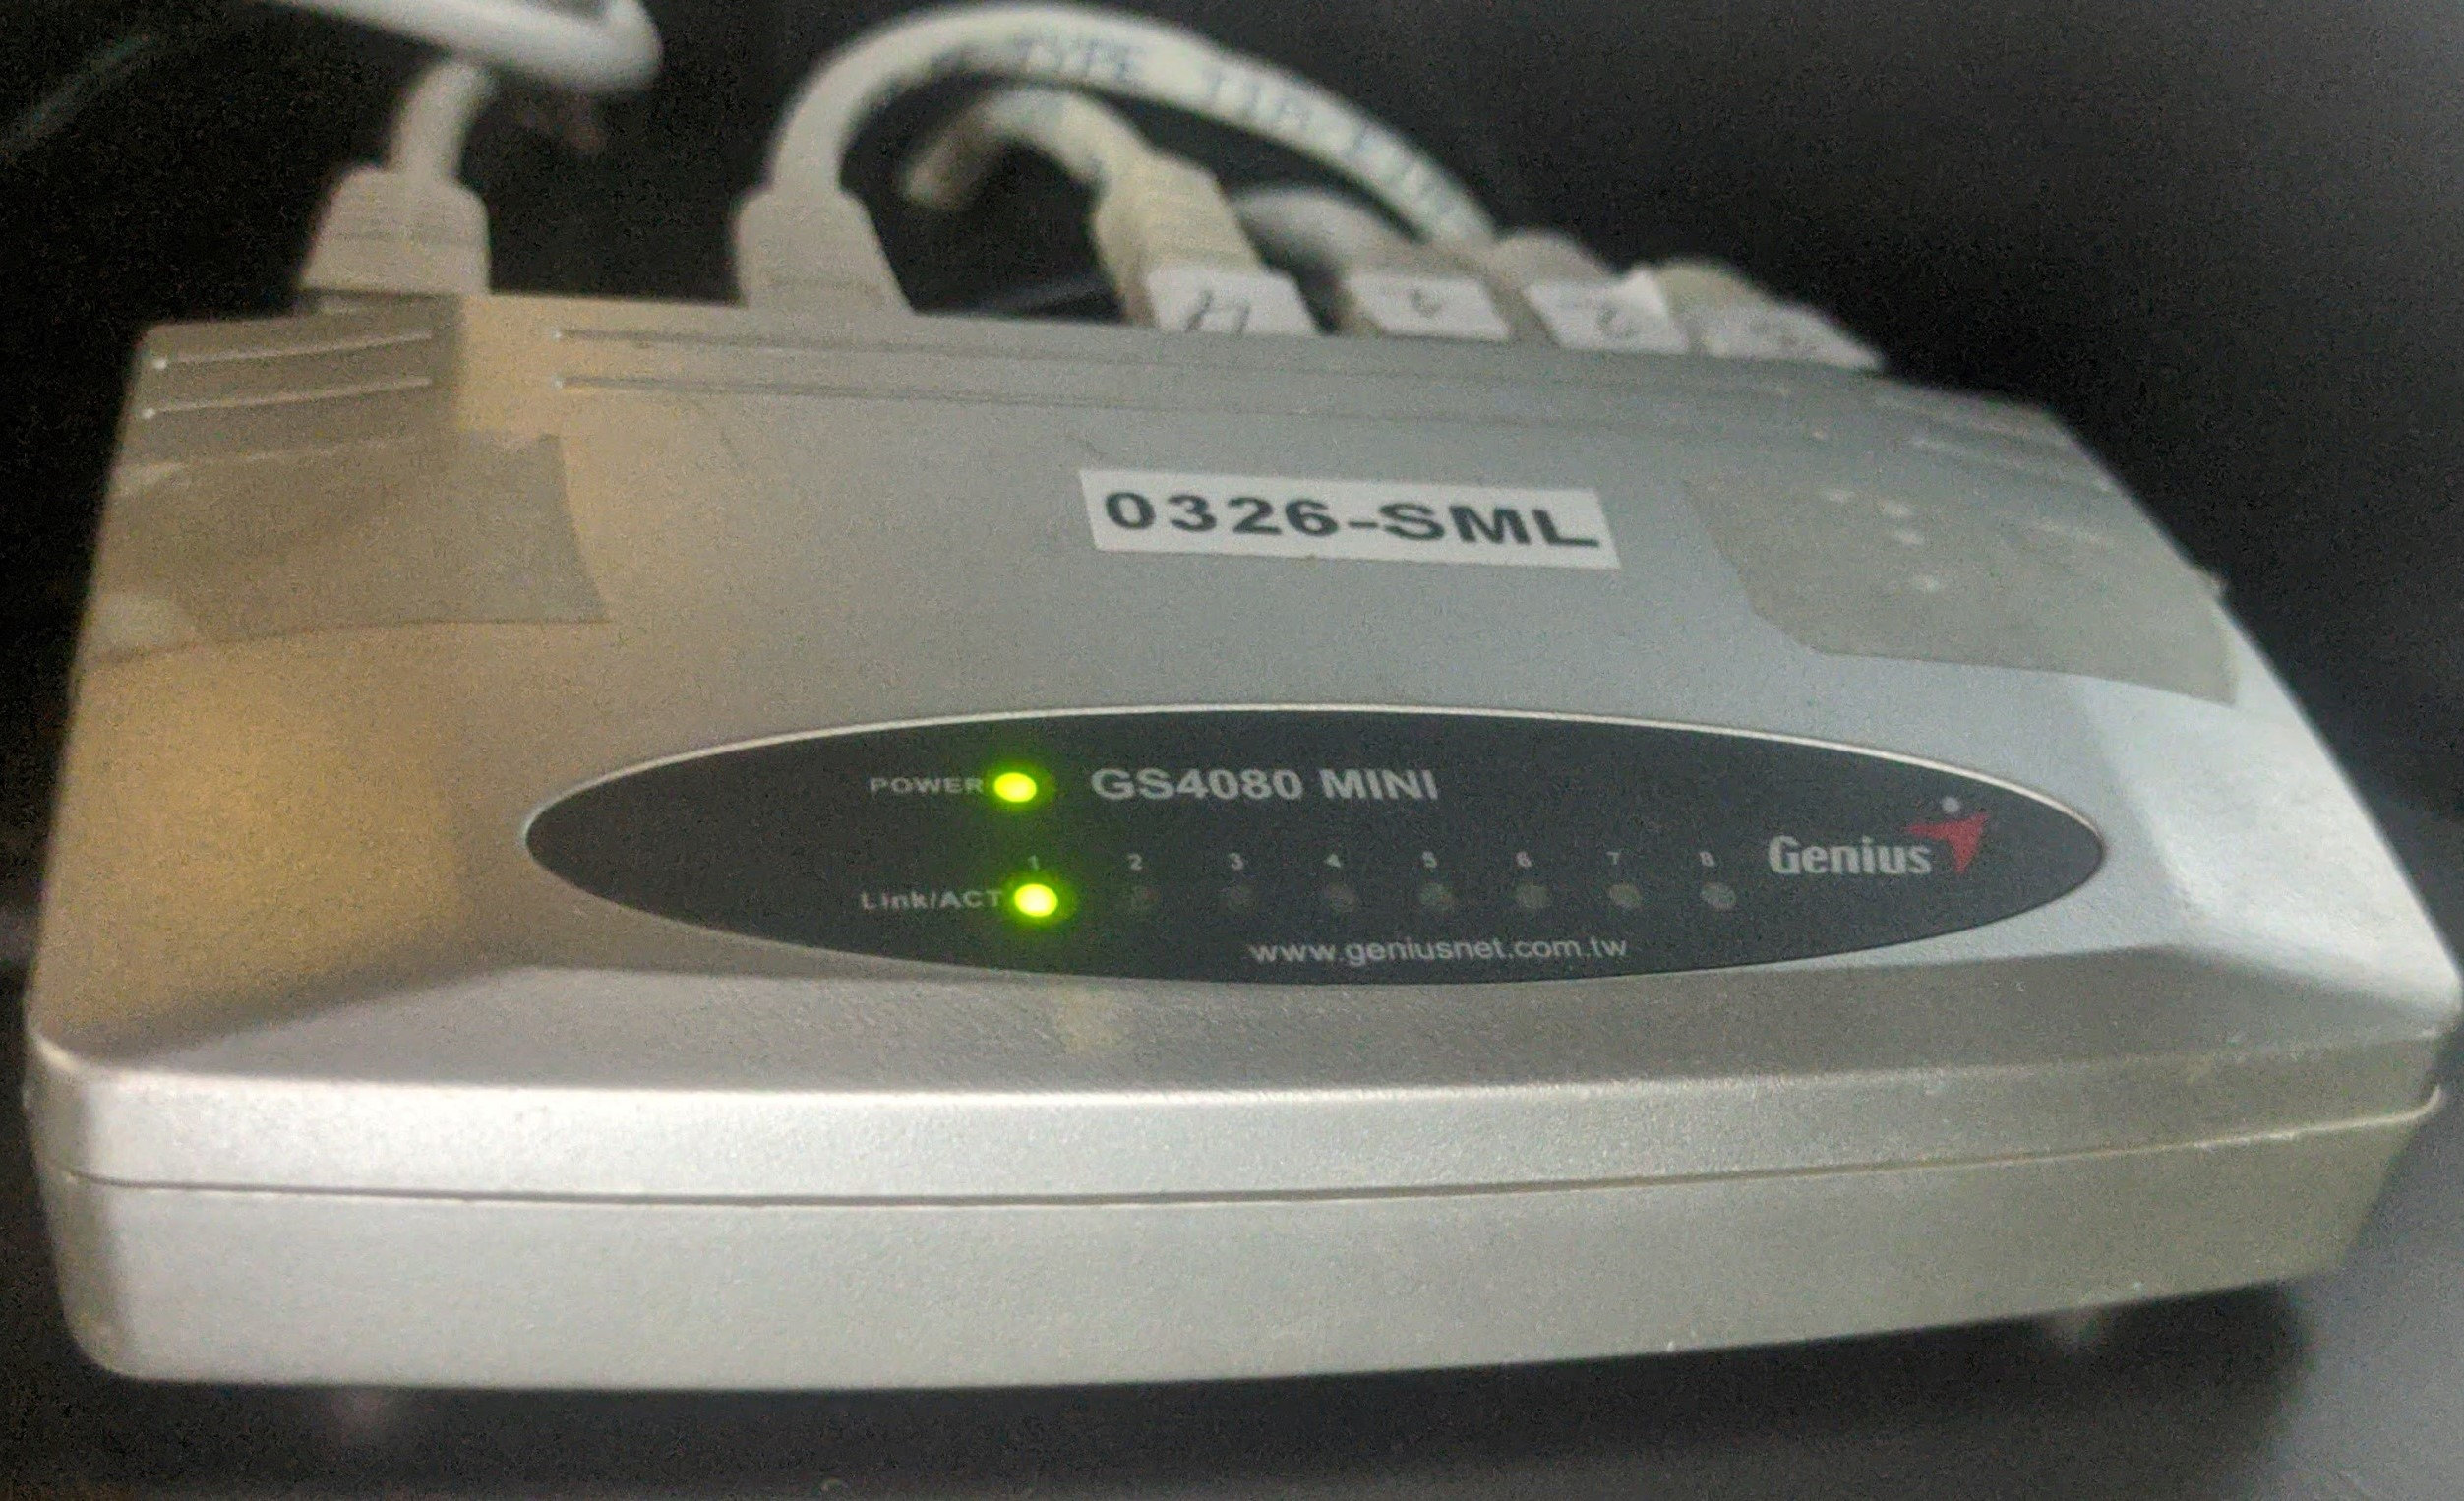
\includegraphics[height=0.2\textheight]{Figuras/switch.jpg}
        \caption{Montaje del switch} 
    \end{minipage}

    \includegraphics[width=0.75\textwidth]{Figuras/raspberrys.jpg}
    \caption{Montaje de las Raspberries}     
\end{figure}

La Jetson Nano y cada Raspberry tienen un cable ethernet conectado al switch, el cual, a su vez, cuenta con otro cable ethernet por el cual se conecta al router (no visible en las fotos).

\newpage
\subsection{Datos involucrados}
Al tratarse este proyecto de una modificación del sistema de recomendación de R.Sánchez y col., se heredarán todos los datos. Cabe mencionar que R.Sánchez y col. utilizaron información proporcionada por el proyecto Green Soul\autocite{EcoawarePersuasiveNetworked} para crear su sistema de recomendación. El proyecto Green Soul trataba de persuadir a los usuarios para que aumentase su conciencia energética y cambiaran sus hábitos de consumo, para ello, se realizaron una serie de encuestas donde se les preguntaba a los usuarios por sus datos personales y se les pedía que ordenarán en función de su criterio qué estrategias de persuasión les parecían más efectivas.
\\ \\
Por tanto, las estrategias de persuasión que se recomiendan pertenecen al ámbito de la concienciación del consumo energético, aunque podrían ser extrapolables a otros casos. De todas formas, se eludirán los detalles sobre estas estrategias ya que no son el caso de estudio y no entran en el alcance de este proyecto.
\\ \\
Teniendo en cuenta todo lo anterior, este capítulo se ha redactado para entender la gestión de los datos en este proyecto, ya que algunos son de carácter personal y es de suma importancia preservar su privacidad. Estos datos se pueden dividir en tres categorías:
\begin{itemize}
    \item \textbf{No sensibles}, la información de los elementos a recomendar, que no son ni personales ni suministrados por ninguna persona.
    \item  \textbf{Sensibles}, datos que hacen referencia a información personal o que son proporcionados por las personas involucradas en el cuestionario.
    \item \textbf{Sintéticos}, datos de usuarios generados aleatoriamente para paliar la necesidad de datos personales del modelo de consenso (sección \ref{Consenso}.Agregación de modelos por consenso).
\end{itemize} 

\subsubsection{No sensibles}
Como se ha mencionado antes, en la categoría de datos no sensibles se encuentran los datos que no son personales ni hacen referencia a ningún usuario. En esta categoría únicamente aparecen aquellos datos que hacen referencia a los elementos que se van a recomendar en el sistema y sus atributos.
\\ \\
Cada estrategia de persuasión que pueda recomendar el RS contará con hasta dos atributos, para que de esta forma, el sistema pueda conocer mejor las estrategias y realizar recomendaciones más precisas en base a esta información. En la tabla \ref{tab:EstrategiasPersuasion} se muestran las estrategias de persuasión involucradas en el RS y sus atributos.
\begin{table}[H]
    %Con esta función se inicia el entorno tabla, que se puede posicionar con respecto al texto al igual que una imagen.
    
    \begin{center}
    %Se centra la tabla.
        \begin{tabular}{|c|p{0.45\linewidth}|p{0.2\linewidth}|p{0.2\linewidth}|}
            % -------------
            \hline
            \rowcolor{Cyan} 
            % -------------
            \textbf{ID} & \textbf{Descripción} & \textbf{Atributo 1} & \textbf{Atributo 2} \\ 
            % -------------
            \hline
            \textbf{V2} &  Reconocimiento público/social de mi contribución al ahorro de energía. & Reconocimiento social & -\\
            % -------------
            \hline
            \rowcolor{GrisTabla}
            \textbf{V5} & Recibir información relacionada con la energía de una forma simple y estéticamente atractiva. & Atractivo físico & -\\
            % -------------
            \hline
            \textbf{V6} &  Recibir beneficios como recompensa por mejorar mi rendimiento energético(horarios de trabajo flexibles, saltarse ciertas tareas, etc.). & Condicionamiento & -\\
            % -------------
            \hline
            \rowcolor{GrisTabla} 
            \textbf{V7} & Recibir un reconocimiento por lograr ahorros de energía de manera colectiva yo y mi equipo. & Reciprocidad & Reconocimiento social\\
            % -------------
            \hline
            \textbf{V10} & Mis altos gerentes están comprometidos con el ahorro de energía. & Autoridad & Demostración social \\
            % -------------
            \hline
            \rowcolor{GrisTabla} 
            \textbf{V11} & Poder monitorear mi propio desempeño energético en tiempo real. & Monitorización propia. & - \\ 
            % -------------
            \hline
            \textbf{V15} &  Información sobre el efecto que mis acciones pueden tener sobre el consumo de energía. & Causa efecto & -\\
            % -------------
            \hline
            \rowcolor{GrisTabla} 
            \textbf{V17} & Evacuación comparativa de mi desempeño en el ahorro de energía respecto a usuarios parecidos a mí. & - & -\\
            % -------------
            \hline
            \textbf{V19} &  Consejos y sugerencias sobre el ahorro de energía al día o a la semana.  & Sugerencia & -\\
            % -------------
            \hline
            \rowcolor{GrisTabla} 
            \textbf{V20} &  Avances y consejos sobre las lecciones aprendidas de usuarios parecidos mí en acciones específicas de ahorro de energía. & Similaridad & -\\
            \hline

            % \rowcolor{Naranja} 
            % \textbf{V} & \textbf{elit} \\ \hline
        \end{tabular}
        \caption{\centering Estrategias de persuasión del sistema (Fuente: Elaboración propia).}
        \label{tab:EstrategiasPersuasion}
    \end{center}    
\end{table}


\subsubsection{Sensibles}
En cuanto a los datos sensibles hay que mencionar dos grupos, los datos personales de los usuarios y los rankings de los usuarios. Este primer grupo está formado por los datos personales de los usuarios participantes, que intervienen en dos puntos clave: en el entrenamiento de los modelos de IA y a la hora de agregar estos modelos. El grupo de los datos de los rankings está formado por las preferencias de los anteriores usuarios a la hora de ordenar las estrategias de persuasión, es decir, el ranking de estrategias para cada usuario.
\\ \\
Tanto los datos personales de los usuarios como los datos de los rankings de estos son necesarios para entrenar un modelo de IA. Los atributos de los usuarios, al igual que los atributos de las estrategias de persuasión, sirven para relacionar los distintos usuarios entre sí y encontrar relación entre sus diferentes atributos con el orden que le han dado a las diferentes estrategias de persuasión, de esta forma, se pueden realizar recomendaciones en base al tipo de usuario.

\paragraph{Datos de usuarios\\}
Los datos personales de los usuarios que intervienen en este proyecto son los presentes en la tabla \ref{tab:AtributosUsuarios}. Estos datos han sido transformados a objetos json para su posterior utilización, formando una lista de objetos en los que cada uno representa los datos personales de un usuario.
\begin{table}[H]
    %Con esta función se inicia el entorno tabla, que se puede posicionar con respecto al texto al igual que una imagen.
    
    \begin{center}
    %Se centra la tabla.
        \begin{tabular}{|c|c|p{0.7\linewidth}|}
            % -------------
            \hline
            \rowcolor{Cyan} 
            % -------------
            \textbf{ID} & \textbf{Nombre} & \textbf{Descripción}\\ 
            % -------------
            \hline
            \textbf{0} &  Edad & Rango de edad\\
            % -------------
            \hline
            \rowcolor{GrisTabla}
            \textbf{1} & Género & Género\\
            % -------------
            \hline
            \textbf{2} & Educación & Nivel educativo\\
            % -------------
            \hline
            \rowcolor{GrisTabla} 
            \textbf{3} & País & País de residencia\\
            % -------------
            \hline
            \textbf{4} & Cultura de trabajo & Cultura de trabajo\\
            % -------------
            \hline
            \rowcolor{GrisTabla} 
            \textbf{5} & PST & Tipo de perfil de usuario en base a los propuestos por Dan Lockton\autocite{locktonModelsUserDesigners2012} : \textit{"Pinball, Shortcut, Thought-ful"}\\ 
            % -------------
            \hline
            \textbf{6} & Barreras  & Barreras ante el cambio\\
            % -------------
            \hline
            \rowcolor{GrisTabla} 
            \textbf{7} & Intenciones & Intenciones ante el cambio\\
            % -------------
            \hline
            \textbf{8} & Confianza  & Confianza ante el cambio\\
            % -------------
            \hline

            % \rowcolor{Naranja} 
            % \textbf{V} & \textbf{elit} \\ \hline
        \end{tabular}
        \caption{\centering Atributos de los usuarios que participan en el sistema (Fuente: Elaboración propia).}
        \label{tab:AtributosUsuarios}
    \end{center}    
\end{table}
\paragraph{Rankings\\}
Los usuarios, a parte de introducir sus datos personales anteriores, también introducen el orden de las estrategias de persuasión en base a la relevancia que consideran que tienen. Este ranking de estrategia es recogido y transformado a formato json formando una lista de objetos json en la que cada objeto representa los datos de la tabla \ref{tab:RankingUsuario}.
\begin{table}[H]
    \begin{center}
    %Se centra la tabla.
        \begin{tabular}{|c|p{0.7\linewidth}|}
            % -------------
            \hline
            \rowcolor{Cyan} 
            % -------------
            \textbf{Nombre} & \textbf{Descripción}\\ 
            % -------------
            \hline
            \textbf{User ID}  & Identificador único del usuario\\
            % -------------
            \hline
            \rowcolor{GrisTabla}
            \textbf{Item ID}  & Identificador único de la estrategia de persuasión\\
            % -------------
            \hline
            \textbf{Ranking} & Valor en el ranking de la estrategia de persuasión\\
            % -------------
            \hline
            % \rowcolor{Naranja} 
            % \textbf{V} & \textbf{elit} \\ \hline
        \end{tabular}
        \caption{\centering Elementos de la estructura de los datos del ranking  (Fuente: Elaboración propia).}
        \label{tab:RankingUsuario}
    \end{center}    
\end{table}


\subsubsection{Sintéticos}
En cuanto a los datos sintéticos, se debe tener en cuenta que los datos sensibles han sido directamente suministrados por los usuarios, por lo cual, es técnicamente imposible acceder a ellos desde el servidor de agregación, ya que sería una evidente violación de la privacidad de los usuarios. Esto genera un gran problema debido a que el propio modelo de consenso, explicado en la sección \ref{Consenso}, requiere de datos de usuarios para funcionar.
\\ \\
La forma de abordar el problema de la necesidad de datos es mediante la creación de usuarios sintéticos, como se explica en la subsección \ref{Consenso:Usuarios_Sinteticos}. Estos usuarios sintéticos tendrán los mismos atributos que los usuarios normales (tabla \ref{tab:AtributosUsuarios}), tendrán que clasificar las mismas estrategias de persuasión (tabla \ref{tab:EstrategiasPersuasion}) y el ranking se gestionará de la misma forma (tabla \ref{tab:RankingUsuario}).

\newpage
\subsection{Protocolo de Federated Learning}\label{Protocolo}
El protocolo de Federated Learning que se va a reproducir en este proyecto es una adaptación de lo que proponen K. Bonawitz y col. \autocite{bonawitzFederatedLearningScale2019a}. En este protocolo se definen tres fases importantes, la selección de participantes, la configuración del mecanismo de agregación y el envío reporte de cada participante.
\\\\
Para este caso se han introducido leves cambios en este protocolo que se irán explicando en las sucesivas partes del mismo.  

\subsubsection{Selección de participantes}
La selección de participantes al tratarse de un caso de estudio concreto no se limita ni se controla de ninguna forma, simplemente se ha implementado una red en la que participan cuatro dispositivos diferentes.

\subsubsection{Intercambio de claves}
El intercambio de claves es una de las novedades introducidas sobre el protocolo previamente mencionado, en este paso, el objetivo es que los diferentes dispositivos de la red compartan sus claves públicas para poder asegurar la privacidad de la red, imagen \ref{fig:PublicKeyShare}. 
\\ \\
La utilización de estas claves públicas y su función están definidas en el apartado de securización de las comunicaciones \ref{SegCom}.
\begin{figure}[H]
    \centering
    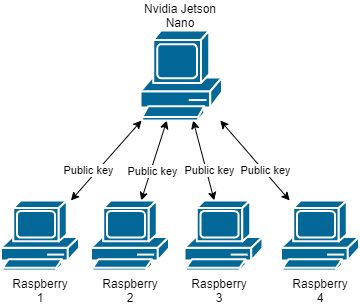
\includegraphics[width=0.5\textwidth]{Figuras/Network_public_key.png}    
    \caption{Intercambio de claves públicas entre los participantes} 
    \label{fig:PublicKeyShare}
\end{figure}

\subsubsection{Entrenamiento}
El entrenamiento es algo que en el protocolo se omite pero que es importante mencionar. Este proceso se lleva a cabo en el dispositivo del participante y conlleva dos tareas:
\begin{itemize}
    \item En primer lugar este participante crea su modelo de IA, lo entrena con los datos que él elija y lo almacena.
    \item En segundo lugar este modelo es cifrado y enviado al servidor. El proceso de cifrado se puede observar en el diagrama \ref{fig:Flow_Encryption} de la sección de securización de las comunicaciones \ref{SegCom}.
\end{itemize} 
\begin{figure}[H]
    \centering
    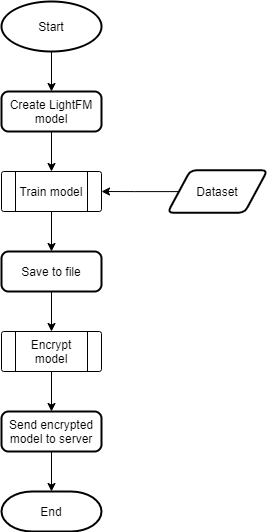
\includegraphics[height=0.6\textheight]{Figuras/flowchart_train.png}    
    \caption{Intercambio de claves públicas entre los participantes} 
    \label{fig:Entrenamiento}
\end{figure}

\subsubsection{Comunicación con el servidor}
La comunicación con el servidor es un proceso crucial en el que se debe asegurar que los modelos de los participantes lleguen sin modificaciones y sin ser interceptados por ningún atacante. Para detallar este proceso se ha elaborado una sección donde se explican más a fondo los pasos llevados para conseguir que las comunicaciones sean seguras, sección \ref{SegCom}.
\\ \\
Debido a este protocolo de seguridad, los participantes deberán enviar tanto los modelos cifrados como las claves cifradas, como se puede observar en las siguientes imágenes.

\begin{figure}[H]
    \begin{minipage}[t]{0.45\linewidth}  % <---
        \centering
        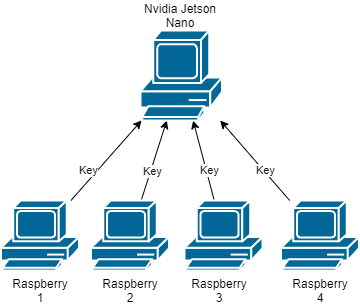
\includegraphics[width=\textwidth]{Figuras/Network_participant_encrypted_key.png}
        \caption{Envío de la clave de cifrado del modelo al servidor de agregación} 
    \end{minipage}
    \hfill
    \begin{minipage}[t]{0.45\linewidth}  % <---
        \centering
        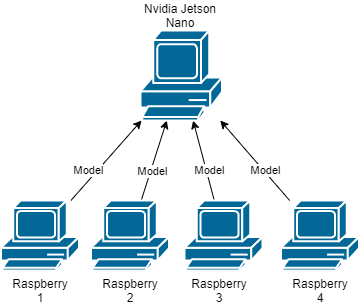
\includegraphics[width=\textwidth]{Figuras/Network_participant_encrypted_model.png}    
        \caption{Envío del modelo cifrado al servidor de agregación} 
    \end{minipage}
\end{figure}

\subsubsection{Agregación de los modelos}
En este proceso, como tal, no va a ocurrir una agregación de modelos, sino más bien una compartición de conocimiento de forma indirecta mediante el modelo de consenso. Este sistema está explicado con detalle en la sección \ref{Consenso} de este capítulo.
\\ \\
De todas formas, para verlo de una forma más sencilla, se puede observar el siguiente diagrama \ref{fig:Flow_Agregation} en el cual se muestra el flujo de los datos y de los modelos para ser agregados. El proceso que recorre este diagrama puede ser dividido en 4 partes:
\begin{itemize}
    \item Se reciben los modelos de los participantes (en este caso 4), se descifran siguiendo el diagrama \ref{fig:Flow_Decryption} (explicado con detalle en en la sección de securización de las comunicaciones \ref{SegCom}) y se guardan los modelos para su posterior utilización.
    \item Una vez se cuente con los modelos descifrados, se generan los usuarios sintéticos, después, con el modelo de cada participante se realiza la predicción del ranking para estos usuarios y se almacena para su posterior utilización. 
    \item Mediante el modelo de consenso explicado en el apartado \ref{Consenso} estas predicciones son convertidas a una única predicción por usuario sintético generado. Después, la información se almacena para su uso final.
    \item Por último, se coge toda la información de los usuarios sintéticos y los rankings consensuados para reentrenar el modelo de cada participante. 
\end{itemize}
\begin{figure}[H]
    \centering
    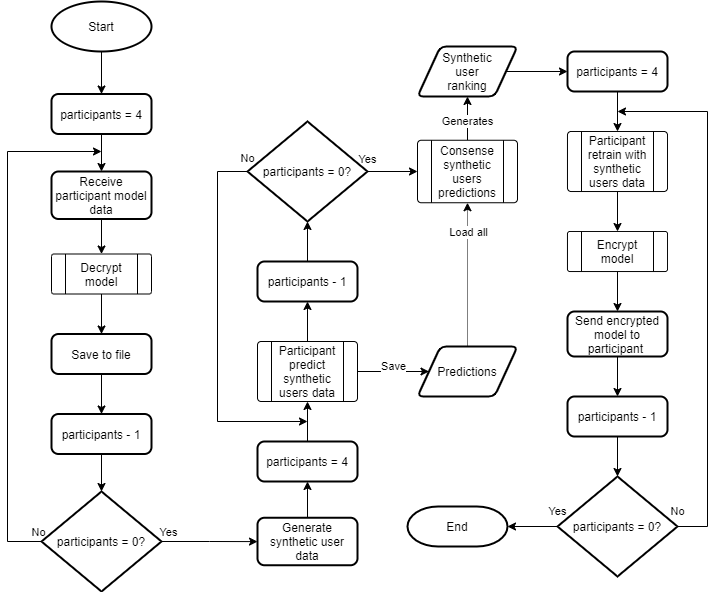
\includegraphics[width=\textwidth]{Figuras/flowchart_agregation.png}    
    \caption{Diagrama del flujo de reentrenado de los modelos} 
    \label{fig:Flow_Agregation}
\end{figure}
\newpage
\subsubsection{Comunicación con los participantes}
La comunicación con los participantes se realiza de la misma forma que los participantes se comunican con el servidor, la única diferencia es que el receptor en este caso son los participantes.
\begin{figure}[H]
    \begin{minipage}[t]{0.45\linewidth}  % <---
        \centering
        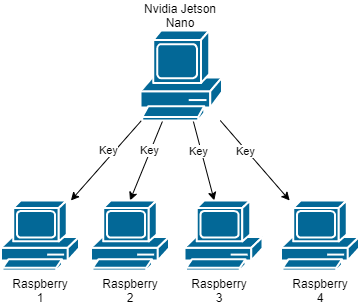
\includegraphics[width=\textwidth]{Figuras/Network_node_encrypted_key.png}
        \caption{Envío de la clave de cifrado del modelo de cada participante a cada participante} 
    \end{minipage}
    \hfill
    \begin{minipage}[t]{0.45\linewidth}  % <---
        \centering
        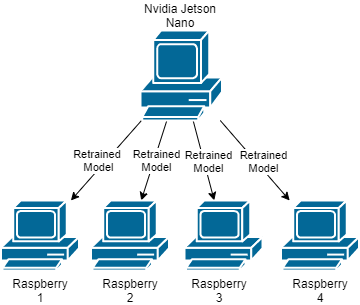
\includegraphics[width=\textwidth]{Figuras/Network_node_encrypted_model.png}    
        \caption{Envío de cada modelo cifrado a su correspondiente dueño} 
    \end{minipage}
\end{figure}
\subsubsection{Comparación de modelos}
En el momento que el modelo llega al participante este tiene que valorar si realmente le supone una mejora o no, para ello como puede verse en el diagrama \ref{fig:Flow_Compare}, existen varias fases a llevar a cabo.

En primer lugar, al igual que como con el servidor de agregación, se debe descifrar el modelo recibido. Después, compararlo con el modelo del participante, esto se puede hacer tratando de analizar la precisión de las predicciones para varios subconjuntos de datos de test con los que cuente el dispositivo. En resumen, predecir para los usuarios existentes de su ranking con los dos modelos y quedarse con el modelo que más acierte.

\begin{figure}[H]
    \centering
    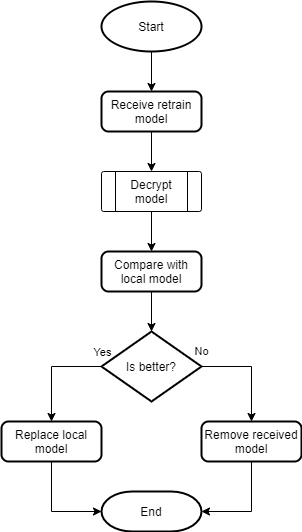
\includegraphics[height=0.6\textheight]{Figuras/flowchart_compare.png}    
    \caption{Diagrama del flujo de la comparación de los modelos} 
    \label{fig:Flow_Compare}
\end{figure}

\newpage
\subsection{Securización de las comunicaciones}
Para preservar la seguridad y privacidad en el protocolo de aprendizaje federado propuesto es imprescindible securizar las comunicaciones. Para securizarlas se han llevado a cabo dos acciones clave, la primera en lo que concierne al protocolo de comunicación y la segunda en cuanto al cifrado de la comunicación.

\subsubsection{Protocolo de comunicación}
En cuanto al protocolo de comunicación se ha optado por la utilización del protocolo SCP (Secure Copy Protocol), conocido en español como protocolo de copia segura. Este protocolo requiere del protocolo SSH (Secure Shell), conocido en español como terminal seguro.
\\ \\
El protocolo SSH permite el acceso remoto a un servidor o dispositivo por un canal seguro a través de una clave. Además, el protocolo usa técnicas de cifrado que impiden que la información que viaje en la red lo haga de forma legible. El protocolo SCP permite la transferencia de archivos entre dispositivos de la red usando el protocolo SSH como base.

\subsubsection{Cifrado de la comunicación}
Aunque las comunicaciones en el protocolo SCP y SSH vayan cifradas son susceptibles de ser atacadas. Para mejorar este aspecto se ha realizado un sistema de cifrado de los modelos que viajen por la red para preservar la privacidad y seguridad de los participantes.
\\ \\ 
Para esta labor se han utilizado el método criptográfico de criptografía híbrida, que usa tanto la criptografía simétrica como asimétrica.

\paragraph{Cifrado simétrico} 
El cifrado simétrico es aquel sistema de cifrado en el que la misma clave sirve para cifrar como para descifrar el mensaje. 
\\ \\
El problema de este sistema es que toda la seguridad reside en la clave empleada en el cifrado. Esto es un gran impedimento a la hora de gestionar comunicaciones debido al cómo gestionar el envío de esta clave, ya que si no se hace por un canal seguro el mensaje sera fácilmente descifrable.
\\ \\
Por otro lado, este sistema cuenta con dos grandes ventajas, es sencillo, es rápido y requiere menos recursos para llevarlo a cabo.

\paragraph{Cifrado asimétrico}
El cifrado asimétrico es aquel sistema de cifrado que consta de dos claves criptográficas, una pública y una privada. La clave pública es utilizada para cifrar el mensaje mientras que la privada es utilizada para descifrarlo. 
\\ \\
Este sistema cuenta con tres grandes desventajas que impiden su uso en exclusivo o su uso con grandes volúmenes de información a cifrar. 
\begin{itemize}
    \item Se necesita más procesado de computo para generar la clave.
    \item Las claves asimétricas son mucho más grandes que las simétricas.
    \item El mensaje cifrado ocupa más espacio que el original.
\end{itemize}

Debido a que los dispositivos con los que se cuenta no tienen una gran capacidad de computo no se podría establecer un tamaño de clave lo suficientemente grande como para poder cifrar el modelo de inteligencia artificial completo. Este modelo pesa al rededor de los 7Kb y para cifrarlo con este sistema habría que generar una clave del mismo tamaño mayor.
\\ \\
Sin embargo, este sistema al constar de dos claves independientes es más sencillo salvaguardar la privacidad y seguridad de los integrantes.

\paragraph{Cifrado híbrido}
Teniendo en cuenta los anteriores dos tipos de cifrado se decidió utilizar el sistema híbrido para obtener los resultados más óptimos, protegiendo la privacidad y pudiendo realizar las tareas de cifrado desde dispositivos con menor capacidad computacional.
\\ \\ 
El proceso de cifrado se ha realizado de acorde al diagrama de flujo representado en la figura \ref{fig:Flow_Encryption}. En este diagrama se pueden observar los pasos que se han realizado para la encriptación de la información, en primer lugar el modelo de LightFM se convertió a bytes y se comprimió para reducir el volumen de datos a enviar por la red, pudiendo agilizar así las comunicaciones. Después se cifró simétricamente, generando una clave y un mensaje cifrado. Por un lado este mensaje cifrado sería comprimido y se guardaría en un fichero para su posterior envío. Por otro lado, la clave de cifrado simétrica se encriptó asimetricamente con la clave pública del receptor del mensaje, dando como resultado una clave de cifrado simétrico cifrada asimetricamente. Esta clave sería guardada en un fichero para ser enviada al igual que el mensaje.
\begin{figure}[H]
    \centering
    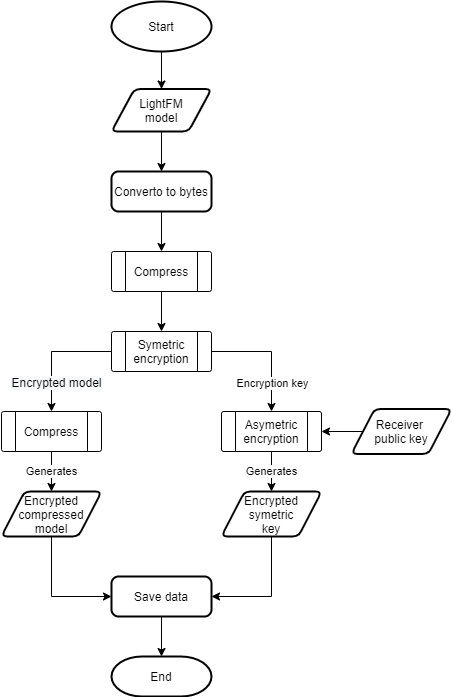
\includegraphics[height=0.6\textheight]{Figuras/flowchart_encryption.png}    
    \caption{Diagrama de flujo del proceso de cifrado} 
    \label{fig:Flow_Encryption}
\end{figure}


\subsubsection{Descifrado del mensaje}
El descifrado del mensaje es el proceso inverso al cifrado de la figura \ref{fig:Flow_Encryption}. Para ello, en un primer momento se reciben tanto el modelo cifrado simétricamente como la clave del modelo cifrada asimétricamente. En primer lugar, la clave que se ha recibido se descifra asimétricamente con la clave privada propia, ya que esta solo es descifrable por el receptor. Una vez descifrada la clave, se descomprime el modelo y se descifra con esta. Por último, el resultado es descomprimido y convertido a objeto LightFM para su posterior utilización. 
\begin{figure}[H]
    \centering
    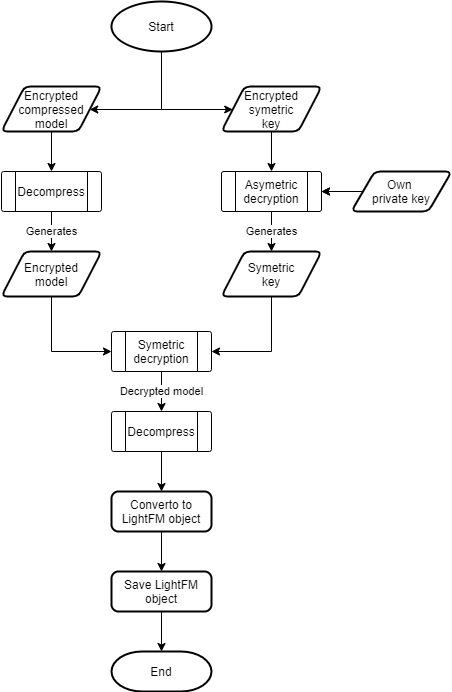
\includegraphics[height=0.6\textheight]{Figuras/flowchart_decryption.png}    
    \caption{Diagrama de flujo del proceso de descifrado} 
    \label{fig:Flow_Decryption}
\end{figure}
\newpage
\subsection{Agregación de modelos por consenso}\label{Consenso}
A la hora de agregar los diferentes modelos de los participantes se estudiaron los distintos algoritmos de los sistemas de FL, pero todos tenían algo en común, accedían a los datos del modelo. Aunque estos datos de los modelos sean meras matrices y números, el objetivo de este proyecto era no acceder en ningún momento a la información presente en ellos, por lo que se buscó otra solución.
\\ \\
La solución llegó con un cambio de enfoque. Se dejó de combinar los distintos modelos para crear uno global y se pasó a compartir únicamente sus formas de operar. Esto se debe a que en la agregación de modelos se suelen ensamblar los modelos de los distintos participantes. Es decir, se combinan los modelos o se extraen de cada modelo ciertos parámetros para crear uno general. El problema presente en estos enfoques tradicionales es que se accede a la información de los modelos de forma directa, objetivo principal a evitar en este proyecto.
\\ \\
El enfoque de compartir la forma de operar de los distintos modelos de IA se empezó a explorar mediante la generación de usuarios sintéticos, para los cuales, el modelo de cada participante de la red de FL debería predecir su ranking. Cuando cada participante predice el ranking para cada usuario sintético están demostrando cómo actuarían ante ciertas entradas de datos, por lo que si se compartiera este conocimiento, los participantes se verían beneficiados de las formas de operar de otros participantes.
\\ \\
El problema es que, desde un punto de vista objetivo, puede que algunas formas de operar no sean del todo \textit{precisas}, por lo que no se debería compartir los rankings predichos por todos los modelos sin ningún tipo de filtrado. Para realizar este filtrado y con el objetivo de llegar a un punto intermedio se creó el modelo de consenso, en el cual las predicciones que da cada modelo para los usuarios sintéticos se combinan de forma que todos los modelos lleguen a un acuerdo para el ranking de cada usuario. 
\\ \\
Este modelo de consenso se explicará en los siguientes apartados, donde se enseñará cómo se generan los datos sintéticos, como se generan los rankings, las explicaciones matemáticas del consenso y el proceso de reentrenado de los modelos.

\subsubsection{Generar datos personales sintéticos}\label{Consenso:Usuarios_Sinteticos}
Uno de los elementos imprescindibles para poner en práctica el sistema de agregación por consenso, es la necesidad de datos de usuarios, que con el objetivo de evitar cualquier violación de privacidad serán creados en el servidor, siendo de ahora en adelante denominados como usuarios sintéticos.
\\ \\
Estos usuarios sintéticos tendrán los mismos atributos que cualquier usuario del sistema, es decir, contarán con todos los atributos presentes en la tabla \ref{tab:AtributosUsuarios}. Como ya se ha dicho antes, el proceso de creación de estos datos es crucial para el correcto funcionamiento del sistema, ya que si los usuarios generados fueran de un perfil concreto, el aprendizaje no sería favorable para todos los participantes de la red, puesto que lo más seguro es que únicamente el participante con más usuarios de este perfil sea beneficiado, mientras que para los demás participantes, supondrá una pérdida de precisión por el ruido introducido en su modelo. Es por eso que se ha tomado la decisión de generarlos aleatoriamente, evitando así estancarse en perfiles concretos y tratando de favorecer a todos los participantes. 
\subsubsection{Generar ranking de los usuarios}
Los datos de los usuarios sintéticos por sí solos no son suficientes ni para entrenar ni para mejorar ningún modelo de IA, hace falta saber el ranking que estos usuarios sintéticos darían a las diferentes estrategias de persuasión, tabla \ref{tab:EstrategiasPersuasion}. 
\\ \\
Esta cuestión no puede ser abordada aleatoriamente como la anterior, ya que cada usuario ordena en base a su opinión y sus preferencias las estrategias de persuasión, por lo cual, de hacerlo aleatoriamente, se distorsionaría la realidad y no sería representativo. Además, si este ranking se generase aleatoriamente y se compartiera con los participantes de la red, distorsionaría por completo sus modelos, lo que llevaría a una pérdida inmensa de precisión. 
\\ \\
Es debido a esta problemática que se ha creado el método de consenso. Este método trata de representar la \textit{``opinión''} de cada participante de la red mediante la estimación del ranking para cada usuario sintético. Todas estas \textit{``opiniones''} serán puestas en común mediante el algoritmo de consenso, lo que dará como resultado un ranking por usuario sintético, que será usado con los datos del usuario sintético para reentrenar los modelos.
\newpage
\subsubsection{Consenso}
El proceso de consenso comienza con la ya mencionada creación de usuarios sintéticos aleatoriamente, pero la generación del ranking de estos se lleva a cabo de la siguiente manera.

\paragraph{Estructuras básicas} En primer lugar hay que definir la lista de las estrategias \textit{E} a ser ordenadas por los modelos \textit{m} de los participantes, que en este caso serán las mismas que las de la tabla \ref{tab:EstrategiasPersuasion}. Estas estrategias serán representadas como \textit{e$_{j}$}, siendo \textit{j} la cantidad de estrategias de la lista \textit{E} y \textit{e$_{j}$} la estrategia final de esta lista. 
\[
    \textit{E} = \begin{bmatrix} \textit{e$_{1}$} & \textit{e$_{2}$} & \textit{e$_{3}$} & \textit{e$_{4}$} & \cdots & \textit{e$_{j}$} \end{bmatrix}
\]
A la hora de crear una predicción de ranking, denotada \textit{r}, para las estrategias \textit{e$_j$} $\in$ \textit{E} se representará cada estrategia con un valor \textit{a}, siendo \textit{a} el puesto de la estrategia de persuasión en el ranking. Por lo cual, \textit{a} ha de ser siempre menor o igual que el número total de estrategias y mayor que cero, para así, mantenerse dentro del rango de \textit{E} (0$<$
\textit{a }$\leq$\textit{ j}), puesto que cada predicción \textit{r} no es más que una mera valoración de un usuario de las \textit{j} estrategias \textit{e} de la lista \textit{E}.
\[
    \textit{r} = \begin{bmatrix} \textit{a$_{1}$} & \textit{a$_{2}$} & \textit{a$_{3}$} & \textit{a$_{4}$} & \cdots & \textit{a$_{j}$} \end{bmatrix}
\]
De esta forma, se puede afirmar que el primer elemento del ranking tendrá el valor 1 y el último el valor \textit{j}, quedándose las demás estrategias con el resto de los puestos en ese rango. Lo que en un conjunto de 10 estrategias se traduce en que la mejor estrategia obtendría el valor 1 y la peor el valor 10.
\\ \\
Sin embargo, cuando se trata de realizar varias predicciones se simboliza como una matriz \textit{R}, donde cada predicción es representada por \textit{r$_{i}$}, en el que \textit{r} denota la predicción del ranking  e \textit{i} denota la cantidad de predicciones \textit{r} realizadas.
\[  
    \textit{R} = 
    \begin{pmatrix}
        \textit{r$_{1}$}  \\ 
        \textit{r$_{2}$}  \\ 
        \vdots  \\ 
        \textit{r$_{i}$}
    \end{pmatrix} 
    =
    \begin{pmatrix}
        a_{11}  &  a_{12}  &  \cdots   & a_{1j} \\ 
        a_{21}  &  a_{22}  &  \cdots   & a_{2j}\\ 
        \vdots  &  \vdots  &  \ddots & \vdots  \\ 
        a_{i1}  &  a_{i2}  &  \cdots   & a_{ij}
    \end{pmatrix}
\]
\newpage
\paragraph{Predicción} Una vez entendidas las estructuras básicas que se utilizarán en el método de consenso, este apartado presentará su aplicación, ya que en este apartado se crearán las predicciones que serán consensuadas a posteriori para generar los datos de reentrenamiento.
\\ \\
Se debe tener en cuenta que las operaciones anteriores cambian por completo cuando se realizan predicciones para un conjunto \textit{U} de usuarios, y si además, estas predicciones se hacen con los diferentes modelos \textit{m} de los participantes, las operaciones se complican bastante. 
\\ \\
En primer lugar, se ha de especificar que el conjunto de usuarios \textit{U} estará formado por los \textit{k} identificadores de los usuarios, representados como \textit{u$_{k}$}. Este conjunto de identificadores se crea cuando se generan los datos personales sintéticos y recoge todos los identificadores de todos los usuarios generados aleatoriamente.
\[
        \textit{U} = \begin{bmatrix} \textit{u$_{1}$} & \textit{u$_{2}$} & \textit{u$_{3}$} & \textit{u$_{4}$} & \cdots & \textit{u$_{k}$} \end{bmatrix}
\]
Para realizar las distintas predicciones con el modelo \textit{m} de cada participante de la red de FL, hay que tener en cuenta que las predicciones \textit{R} pertenecerán al modelo \textit{m}, por lo que se denotará a partir de ahora como \textit{R$_{m}$}. Además, esta matriz de predicciones \textit{R$_{m}$} estará formada por las distintas predicciones para los distintos usuarios \textit{u}, lo que será representado como \textit{r$_{u}$}.
\[  \textit{R$_{m}$} = 
    \begin{pmatrix}
        \textit{r$_{1}$}  \\ 
        \textit{r$_{2}$}  \\ 
        \vdots  \\ 
        \textit{r$_{u}$}
    \end{pmatrix} 
    =
    \begin{pmatrix}
        a_{11}  &  a_{12}  &  \cdots   & a_{1j} \\ 
        a_{21}  &  a_{22}  &  \cdots   & a_{2j}\\ 
        \vdots  &  \vdots  &  \ddots & \vdots  \\ 
        a_{u1}  &  a_{u2}  &  \cdots   & a_{uj}
    \end{pmatrix}
\]
\newpage
\paragraph{Redistribución de las predicciones}
Las predicciones realizadas con cada modelo \textit{m} sobre el conjunto de usuarios \textit{U} puede ser interpretada de diferente forma. En un principio se entiende que cada modelo \textit{m} genera una predicción \textit{R} para cada uno de los \textit{u} usuarios generados, pero del mismo modo, se puede entender que cada usuario \textit{u} obtiene una predicción \textit{r} por cada modelo \textit{m} y que con la unión de todas las predicciones \textit{r} de todos los modelos \textit{m} para este mismo usuario \textit{u} se puede construir una matriz \textit{R}. 
\\ \\
Para entender lo anterior con más facilidad se ha de comprender que ya no solo se cuenta con una matriz de predicciones \textit{R}, sino que se cuenta con una matriz \textit{P} con \textit{m} matrices de predicciones \textit{R}, denotada como \textit{P$_{m}$}. Esta matriz representa todas las predicciones \textit{R} realizadas por cada modelo \textit{m} participante en la red de FL para un mismo conjunto de usuarios \textit{U}.
\[
    \textit{P$_{m}$}=
    \begin{pmatrix}
        \begin{pmatrix}
            a_{11}  &  a_{12}  &  \cdots   & a_{1j} \\ 
            a_{21}  &  a_{22}  &  \cdots   & a_{2j}\\ 
            \vdots  &  \vdots  &  \ddots & \vdots  \\ 
            a_{u1}  &  a_{u2}  &  \cdots   & a_{uj}
        \end{pmatrix}_{\textit{1}}
        & 
        \cdots 
        &
        \begin{pmatrix}
            a_{11}  &  a_{12}  &  \cdots   & a_{1j} \\ 
            a_{21}  &  a_{22}  &  \cdots   & a_{2j}\\ 
            \vdots  &  \vdots  &  \ddots & \vdots  \\ 
            a_{u1}  &  a_{u2}  &  \cdots   & a_{uj}
        \end{pmatrix}_{\textit{m}}
    \end{pmatrix}
\]
Teniendo en cuenta esta estructura de datos, la separación de los usuarios ha de hacerse tomando cada predicción \textit{r$_{u}$} de cada participante de forma separada, uniendo las que corresponden al mismo usuario \textit{u} en una nueva matriz de predicciones \textit{R}, que al pertenecer al usuario \textit{u} será denotada como \textit{R$_{u}$}. Cada predicción \textit{r} de \textit{R$_{u}$} es extraída de la predicción \textit{r$_{u}$} de la matriz de predicciones de cada modelo \textit{R$_{m}$}. Además, todas las matrices de predicción \textit{R} de todos los usuarios \textit{u} serán agrupadas bajo el termino \textit{P$_{u}$}. De esta, forma puede afirmarse que \textit{P$_{u}$} está formada por las distintas predicciones \textit{R$_{u}$}, las cuales a su vez están formadas por las distintas predicciones \textit{r$_{u}$} extraídas de \textit{R$_{m}$}.

\[  \textit{R$_{m}$} = 
    \begin{pmatrix}
        a_{11}  &  a_{12}  &  \cdots   & a_{1j} \\ 
        a_{21}  &  a_{22}  &  \cdots   & a_{2j}\\ 
        \vdots  &  \vdots  &  \ddots & \vdots  \\ 
        a_{u1}  &  a_{u2}  &  \cdots   & a_{uj}
    \end{pmatrix}
    \equiv
    \begin{pmatrix}
        \begin{pmatrix} a_{1}  &  a_{2}  &  \cdots   & a_{j} \end{pmatrix}_{1} \\ 
        \begin{pmatrix} a_{1}  &  a_{2}  &  \cdots   & a_{j} \end{pmatrix}_{2} \\ 
        \vdots \\ 
        \begin{pmatrix} a_{1}  &  a_{2}  &  \cdots   & a_{j} \end{pmatrix}_{u}
    \end{pmatrix}
\]
\begin{center}
    Predicciones del modelo \textit{m} para \textit{u} usuarios.
\end{center}
\pagebreak
\[  
    \textit{P$_{m}$}=
    \begin{pmatrix}
        \textit{R$_{1}$} & \textit{R$_{2}$} & \cdots & \textit{R$_{m}$}
    \end{pmatrix}
    \equiv
    \begin{pmatrix}
        \begin{pmatrix}
            \begin{pmatrix} a_{1}  &  a_{2}  &  \cdots   & a_{j} \end{pmatrix}_{1} \\ 
            \begin{pmatrix} a_{1}  &  a_{2}  &  \cdots   & a_{j} \end{pmatrix}_{2} \\ 
            \vdots \\ 
            \begin{pmatrix} a_{1}  &  a_{2}  &  \cdots   & a_{j} \end{pmatrix}_{u}
        \end{pmatrix}_{\textit{1}}
        & 
        \cdots 
        &
        \begin{pmatrix}
            \begin{pmatrix} a_{1}  &  a_{2}  &  \cdots   & a_{j} \end{pmatrix}_{1} \\ 
            \begin{pmatrix} a_{1}  &  a_{2}  &  \cdots   & a_{j} \end{pmatrix}_{2} \\ 
            \vdots \\ 
            \begin{pmatrix} a_{1}  &  a_{2}  &  \cdots   & a_{j} \end{pmatrix}_{u}
        \end{pmatrix}_{\textit{m}}
    \end{pmatrix}
\] 
\begin{center}
    Lista de las predicciones de cada modelo \textit{m} para \textit{u} usuarios.
\end{center}

\[  
    \textit{R$_{u}$} =
        \begin{pmatrix}
            a_{11}  &  a_{12}  &  \cdots   & a_{1j} \\ 
            a_{21}  &  a_{22}  &  \cdots   & a_{2j}\\ 
            \vdots  &  \vdots  &  \ddots & \vdots  \\ 
            a_{m1}  &  a_{m2}  &  \cdots   & a_{mj}
        \end{pmatrix}
        \equiv
        \begin{pmatrix}
            \begin{pmatrix} a_{1}  &  a_{2}  &  \cdots   & a_{j} \end{pmatrix}_{1} \\ 
            \begin{pmatrix} a_{1}  &  a_{2}  &  \cdots   & a_{j} \end{pmatrix}_{2} \\ 
            \vdots \\ 
            \begin{pmatrix} a_{1}  &  a_{2}  &  \cdots   & a_{j} \end{pmatrix}_{m}
        \end{pmatrix}
\]
\begin{center}
    Predicciones para el usuario \textit{u} realizadas por los \textit{m} modelos.
\end{center}

\[  
    \textit{P$_{u}$}=
    \begin{pmatrix}
        \textit{R$_{1}$} & \textit{R$_{2}$} & \cdots & \textit{R$_{u}$}
    \end{pmatrix}
    \equiv
    \begin{pmatrix}
        \begin{pmatrix}
            \begin{pmatrix} a_{1}  &  a_{2}  &  \cdots   & a_{j} \end{pmatrix}_{1} \\ 
            \begin{pmatrix} a_{1}  &  a_{2}  &  \cdots   & a_{j} \end{pmatrix}_{2} \\ 
            \vdots \\ 
            \begin{pmatrix} a_{1}  &  a_{2}  &  \cdots   & a_{j} \end{pmatrix}_{m}
        \end{pmatrix}_{\textit{1}}
        & 
        \cdots 
        &
        \begin{pmatrix}
            \begin{pmatrix} a_{1}  &  a_{2}  &  \cdots   & a_{j} \end{pmatrix}_{1} \\ 
            \begin{pmatrix} a_{1}  &  a_{2}  &  \cdots   & a_{j} \end{pmatrix}_{2} \\ 
            \vdots \\ 
            \begin{pmatrix} a_{1}  &  a_{2}  &  \cdots   & a_{j} \end{pmatrix}_{m}
        \end{pmatrix}_{\textit{u}}
    \end{pmatrix}
\] 
\begin{center}
    Lista de las predicciones para cada usuario \textit{u} realizadas por los \textit{m} modelos.
\end{center}

Para concluir con lo anteriormente explicado, este proceso puede definirse como una transformación de las predicciones que da cada modelo para un grupo de usuarios en las predicciones de cada usuario según cada modelo, \textit{P$_{m}$}$\Longrightarrow $\textit{P$_{u}$}. Además, hay que tener en cuenta que el tamaño de las predicciones de cada usuario depende de la cantidad de modelos que participen en la red de FL, de forma que, cuantos más modelos participen, más predicciones tendrá cada usuario. 
\\ \\
El proceso de transformación de \textit{P$_{m}$} en \textit{P$_{u}$} explicado previamente y representado mediante las matrices, es un proceso que se lleva a cabo en tres partes. Primero, el de definición de las variables necesarias. Segundo, el de predecir los rankings para el conjunto \textit{U} de usuarios con los \textit{m} modelos y el tercero, en el que estas predicciones de los modelos son reordenadas para agruparlas por usuario y no por modelo. El proceso está representado mediante el algoritmo \ref{algth:PreparacionConsenso}.
\\ \\
En este algoritmo la declaración de variables se produce entre las líneas 3 y 9, donde se respeta la nomenclatura utilizada hasta el momento de forma que, si no se entiende alguna variable, se puede acudir a las explicaciones previas para comprender su función. 
\\ \\
Después de esto, se realizan las predicciones de los rankings para todos los usuarios generados sintéticamente, donde \textit{P$_{m}$} está formada por \textit{len(m)} matrices, donde cada matriz \textit{R$_{m}$} representa los de rankings \textit{r$_{m}$} que da el modelo \textit{m} para cada usuario \textit{u}.
\\ \\
Una vez habiendo completado las predicciones con todos los modelos y haber obtenido la lista de matrices \textit{P$_{m}$}, es el momento de agrupar los datos por usuarios \textit{u} en vez de por modelos \textit{m}, \textit{P$_{m}$}$\Longrightarrow $\textit{P$_{u}$}. Para este proceso se recorre la lista de usuarios sintéticos \textit{U} y las predicciones \textit{r$_{u}$} que cada modelo da para cada uno de ellos. De esta forma, se consigue que \textit{P$_{u}$} este formada por \textit{len(U)} matrices, donde cada matriz \textit{R$_{u}$} representa los de rankings \textit{r$_{u}$} que ha dado cada modelo \textit{m} para el usuario \textit{u}. 
\begin{algorithm}[H]
    \caption{Redistribución de las predicciones}\label{algth:PreparacionConsenso}
    \begin{algorithmic}[1]
        \Procedure{Obtener rankings para los usuarios}{}
            \BState \emph{Declaración de las variables necesarias}:
            \State $E \gets [ \dots ]$\Comment{\parbox[t]{0.7\linewidth}{Lista de las estrategias a ordenar}}
            \\
            \State $U \gets [ \dots ]$\Comment{\parbox[t]{0.7\linewidth}{Lista de los identificadores de los usuarios sintéticos}}
            \\
            \State $P_{u} \gets [ len(U) ]$\Comment{\parbox[t]{0.7\linewidth}{Lista de las predicciones de cada usuario}}
            \\
            \State $M \gets [ \dots ]$ \Comment{\parbox[t]{0.7\linewidth}{Lista de los modelos de los participantes}}
            \\
            \State $P_{m} \gets [ len(M) ]$ \Comment{\parbox[t]{0.7\linewidth}{Lista de las predicciones de cada modelo}}
            \\                
            \BState \emph{Predicciones de los modelos}:
            \For {$\textit{int}(participante) \gets 0$ \textbf{to} $\textit{range}(len(M))$}
                \State $R_{m} \gets M[participante].predict(U)$ \Comment{\parbox[t]{0.44\linewidth}{Predecir con el modelo del participante el ranking para los usuarios}}
                \\
                \State $P_{m}[participante] \gets R_{m}$ \Comment{\parbox[t]{0.44\linewidth}{Añadir las predicciones del modelo a la lista de todos los participantes}}
            \EndFor
            \State end \textbf{for};
            \\
            \BState \emph{Redistribución de las predicciones en base a usuarios}:
            \For {$\textit{int}(usuario) \gets 0$ \textbf{to} $\textit{range}(len(U))$}
                \State $R_{u} \gets [\dots]$\Comment{\parbox[t]{0.7\linewidth}{Lista de las predicciones para el usuario}}
                \\
                \For {$\textit{int}(participante) \gets 0$ \textbf{to} $\textit{range}(len(M))$}
                    \State $r_{u} \gets P_{m}[participante][usuario]$ \Comment{\parbox[t]{0.4\linewidth}{Predicción del usuario}}
                    \\
                    \State $R_{u}[participante] \gets r_{u}$ \Comment{\parbox[t]{0.4\linewidth}{Añadir la predicción a la lista de predicciones del usuario}}
                \EndFor
                \State end \textbf{for};
                \\
                \State $P_{u}[usuario] \gets R_{u}$ \Comment{\parbox[t]{0.6\linewidth}{Añadir la lista de predicciones del usuario a la lista de predicciones de todos los usuarios}}
            \EndFor
            \State end \textbf{for};

        \EndProcedure
    \end{algorithmic}
\end{algorithm}

\paragraph{Consensuar predicciones} \label{Consensuar_predicciones} El proceso de consenso es el proceso clave a la hora de agregar los distintos modelos, ya que es gracias a este proceso que se consiguen los datos para reentrenar los modelos. El proceso parte de la lista \textit{P$_{u}$} formada por \textit{len(U)} predicciones \textit{R$_{u}$}, a las cuales se les aplica una función estadística \textit{func()} sobre los \textit{a$_{j, m}$} elementos de los múltiples rankings, convergiendo en un único valor las diferentes listas de rankings. Después de aplicar dicha función sobre todas las columnas \textit{j} de la predicción \textit{R$_{u}$}, se consigue unificar cada columna \textit{j} en un único valor representado como \textit{b$_{j}$}. Con esto se obtiene una única predicción para el usuario \textit{u}, a la cual denotaremos a partir de ahora como \textit{q$_{u}$}. La lista de todas las predicciones consensuadas para el conjunto de usuarios \textit{U} será denotada como \textit{R$_{q}$}.
\[  \textit{R$_{u}$}=
    \begin{pmatrix}
        \begin{pmatrix} a_{1}  &  a_{2}  &  \cdots   & a_{j} \end{pmatrix}_{1} \\ 
        \begin{pmatrix} a_{1}  &  a_{2}  &  \cdots   & a_{j} \end{pmatrix}_{2} \\ 
        \vdots \\ 
        \begin{pmatrix} a_{1}  &  a_{2}  &  \cdots   & a_{j} \end{pmatrix}_{m}
    \end{pmatrix}
    \implies
    \begin{pmatrix}
        \begin{pmatrix} a_{1}  \\  a_{2}  \\  \vdots   \\ a_{m} \end{pmatrix}_{1} & 
        \begin{pmatrix} a_{1}  \\  a_{2}  \\  \vdots   \\ a_{m} \end{pmatrix}_{2} & 
        \cdots &
        \begin{pmatrix} a_{1}  \\  a_{2}  \\  \vdots   \\ a_{m} \end{pmatrix}_{j}
    \end{pmatrix}    
\]
\\
\[  \textit{q$_{u}$} = 
    \begin{pmatrix}
        \textit{func}\begin{pmatrix} a_{1}  \\  a_{2}  \\  \vdots   \\ a_{m} \end{pmatrix}_{1} & 
        \textit{func}\begin{pmatrix} a_{1}  \\  a_{2}  \\  \vdots   \\ a_{m} \end{pmatrix}_{2} & 
        \cdots &
        \textit{func}\begin{pmatrix} a_{1}  \\  a_{2}  \\  \vdots   \\ a_{m} \end{pmatrix}_{j}
    \end{pmatrix}   
\]
\\
\[  \textit{q$_{u}$} = 
    \begin{pmatrix}
        \textit{func}\begin{pmatrix} a_{1}  &  a_{2}  &  \cdots   & a_{m} \end{pmatrix}_{1} & 
        \textit{func}\begin{pmatrix} a_{1}  &  a_{2}  &  \cdots   & a_{m} \end{pmatrix}_{2} & 
        \cdots & 
        \textit{func}\begin{pmatrix} a_{1}  &  a_{2}  &  \cdots   & a_{m} \end{pmatrix}_{j}
    \end{pmatrix}
\]
\\
\[  \textit{q$_{u}$} = 
    \begin{pmatrix}
        b_{1}  &  b_{2}  &  \cdots   & b_{j} 
    \end{pmatrix}
\]
\\
\[ 
    \textit{R$_{q}$} = 
    \begin{pmatrix}
        q_{1}  \\  q_{2}  \\  \vdots \\ q_{u}
    \end{pmatrix}
    \equiv
    \begin{pmatrix}
        \begin{pmatrix}
            b_{1}  &  b_{2}  &  \cdots   & b_{j} 
        \end{pmatrix}_{1}\\
        \begin{pmatrix}
            b_{1}  &  b_{2}  &  \cdots   & b_{j} 
        \end{pmatrix}_{2}\\
        \vdots\\
        \begin{pmatrix}
            b_{1}  &  b_{2}  &  \cdots   & b_{j} 
        \end{pmatrix}_{u}
    \end{pmatrix}
\]
\pagebreak

Las funciones para calcular el valor de consenso \textit{b$_{j}$} que se proponen son las métricas estadísticas de la media(\(\bar{x}\)), mediana(\(\tilde{x}\)) y moda (\(\hat{x}\)). En este proyecto se ha descartado la utilización de la media ya que en caso de que los valores \textit{a$_{j, m}$} fueran muy dispares podría distorsionarse bastante el resultado \textit{b} y perder eficiencia. Por ello, solo se utilizarán las funciones de mediana(\(\tilde{x}\)) y moda (\(\hat{x}\)).
\[  \textit{q$_{u}$} = 
    \begin{pmatrix}
        \widehat{ \begin{pmatrix} a_{1}  &  a_{2}  &  \cdots   & a_{m} \end{pmatrix}_{1}} & 
        \widehat{ \begin{pmatrix} a_{1}  &  a_{2}  &  \cdots   & a_{m} \end{pmatrix}_{2}}& 
        \cdots & 
        \widehat{ \begin{pmatrix} a_{1}  &  a_{2}  &  \cdots   & a_{m} \end{pmatrix}_{j}}
    \end{pmatrix}
\]
\begin{center}
    Representación del consenso por moda
\end{center}    

\[  
    \textit{q$_{u}$} = 
    \begin{pmatrix}
        \widetilde{ \begin{pmatrix} a_{1}  &  a_{2}  &  \cdots   & a_{m} \end{pmatrix}_{1}} & 
        \widetilde{ \begin{pmatrix} a_{1}  &  a_{2}  &  \cdots   & a_{m} \end{pmatrix}_{2}}& 
        \cdots & 
        \widetilde{ \begin{pmatrix} a_{1}  &  a_{2}  &  \cdots   & a_{m} \end{pmatrix}_{j}}
    \end{pmatrix}
\]
\begin{center}
    Representación del consenso por mediana
\end{center}    

Con el objetivo de crear una función de consenso más precisa se elaboró un método híbrido, en el cual se combina tanto la métrica de la moda como la de la mediana, algoritmo \ref{algth:Consensuar}. Este método funciona de la siguiente forma: en primer lugar lee la lista de elementos \textit{a$_{j, m}$} y si existe algún valor duplicado más de \textit{len(m)/2} veces, automáticamente asigna ese valor como \textit{b$_{j}$}, de lo contrario, calculará la mediana de la lista y asignaría ese valor como \textit{b$_{j}$}. Se podrían tomar otras decisiones, ya sea en función de la desviación típica de la lista o incluso desarrollando un algoritmo más complejo para optimizar este proceso, pero dicha tarea se sale del alcance del proyecto.
\\ \\
Como elemento adicional se ha considerado la posibilidad de otorgar un peso al modelo \textit{m} de cualquier participante en concreto, de forma que este tenga más repercusión en el resultado del consenso. Este peso solo será otorgado al modelo que sea más afín al usuario sintético, lo que puede ser calculado por una función o seleccionado por algún atributo en concreto (país, puesto de trabajo, género, etc.). En este caso, este peso se da en función del atributo país, de forma que el modelo del país correspondiente al usuario sintético creado, será el que tenga más trascendencia a la hora de elaborar el ranking consensuado. Este peso será representado como \textit{W$_{c}$} y su valor será un número entero de rango 0 $\leq$ \textit{W$_{c}$} $\leq$ \textit{len(m)/2 +1}. Este rango permite no añadir ninguna importancia extra a ningún modelo \textit{m} o permitir que sea este modelo en exclusiva el que genere el ranking para este usuario \textit{u}, ya que debido a la función de consenso, cuando existen \textit{len(m)/2 +1} veces un valor en una lista de elementos \textit{a$_{j, m}$} este valor es asignado automáticamente por ser la moda.
\\ \\
Este peso se proporciona directamente a la predicción \textit{r$_{u}$} del modelo \textit{m} cuando este genera \textit{R$_{m}$}, al extraerse cada predicción \textit{r$_{u}$} de \textit{R$_{m}$} para formar \textit{R$_{u}$} esta predicción se introducirá \textit{W$_{c}$} veces más en \textit{R$_{u}$}, para que a la hora de aplicar \textit{func()} esta predicción \textit{r$_{u}$} de \textit{R$_{m}$} tenga mayor importancia respecto a la del resto. De esta forma, como se ha dicho antes, si \textit{W$_{c}$} fuese cero, todos los modelos tendrían la misma importancia a la hora de calcular el consenso y si fuera \textit{len(m)/2 +1}, este valor sería la moda y por ello sería su valor directamente asignado a \textit{b$_{j}$}.

\begin{algorithm}[H]
    \caption{Consenso de los datos}\label{algth:Consensuar}
    \begin{algorithmic}[1]
        \Procedure{Realización del consenso}{}
            \BState \emph{Declaración de las variables necesarias}:
            \State $P_{u} \gets [ \cdots ]$\Comment{\parbox[t]{0.7\linewidth}{Lista de las predicciones de cada usuario}}
            \\
            \State $R_{q} \gets [\cdots]$\Comment{\parbox[t]{0.7\linewidth}{Lista de rankings consensuados}}
            \\           
            \BState \emph{Consensuar}:
            \For {$\textit{int}(usuario) \gets 0$ \textbf{to} $\textit{len}(P_{u})$}
                \State $R_{u}  \gets P_{u}[usuario]$ \Comment{\parbox[t]{0.44\linewidth}{Lista de predicciones para un mismo usuario}}
                \\
                \State $columnas, filas  \gets shape(R_{u})$ \Comment{\parbox[t]{0.44\linewidth}{Obtener la forma de la matriz de predicciones}}
                \\
                \State $q_{u} \gets [columnas]$\Comment{\parbox[t]{0.44\linewidth}{Inicializar lista de valores para el ranking consensuado}}
                \\
                \For {$\textit{int}(columna) \gets 0$ \textbf{to} $\textit{columnas}$}
                    \State $ r_{i} \gets R_{u}[:,columna]$ \Comment{\parbox[t]{0.44\linewidth}{Lista de todos los valores de la misma columna}}
                    \\
                    \State $ unicos \gets unique(r_{i})$ \Comment{\parbox[t]{0.44\linewidth}{Cantidad de valores diferentes en la columna}}
                    \\
                    \If{$unicos > len(m)/2 $}
                        \State $q_{u}[columna] \gets \textit{mod}(r_{i} )$\Comment{\parbox[t]{0.44\linewidth}{Asignar valor por moda}}
                    \Else
                        \State $q_{u}[columna] \gets \textit{med}(r_{i} )$\Comment{\parbox[t]{0.44\linewidth}{Asignar valor por mediana}}
                    \EndIf
                    \State end \textbf{if};
                \EndFor
                \State end \textbf{for};
                \State $R_{q}[usuario] \gets q_{u}$\Comment{\parbox[t]{0.44\linewidth}{Guardar valor consensuado en }}
            \EndFor
            \State end \textbf{for};
            \State \textbf{return} $R_{q}$;
        \EndProcedure
    \end{algorithmic}
\end{algorithm}

\newpage

\paragraph{Normalización del consenso}
El problema es que en función de la fórmula que se aplique, el rango de \textit{q$_{u}$} puede que no permanezca dentro del rango de \textit{E}, lo que impide afirmar que el valor \textit{b} de cada estrategia entre dentro del intervalo 0$<$
\textit{a$_{q}$ }$\leq$\textit{ j}. Para solucionar este problema se procesan los valores \textit{a$_{qj}$} de \textit{q$_{u}$}, para que estos permanezcan dentro del rango. Este proceso se realiza intercambiando el valor \textit{a$_{qj}$} menor por el valor del ranking menor disponible, como se puede ver en el algoritmo \ref{algth:NormalizarConsenso}.

\begin{algorithm}[H]
    \caption{Normalización de los datos del consenso}\label{algth:NormalizarConsenso}
    \begin{algorithmic}[1]
        \Procedure{Normalización del consenso}{}
            \BState \emph{Declaración de las variables necesarias}:
            \State $Indice \gets 1$\Comment{\parbox[t]{0.75\linewidth}{Se inicializa el elemento más importante del ranking como 1}}
            \\
            \State $q_{u} \gets [\cdots]$\Comment{\parbox[t]{0.75\linewidth}{Valores del ranking consensuado}}
            \State $aux \gets q_{u}$\Comment{\parbox[t]{0.75\linewidth}{Variable auxiliar}}
            \\                
            \BState \emph{Normalización del consenso}:
            \For {$\textit{int}(i) \gets 0$ \textbf{to} $\textit{len}(aux)$}
                \State $posicion \gets whereIsMin(aux)$ \Comment{\parbox[t]{0.44\linewidth}{Posición de la lista donde está el menor elemento}}
                \\
                \State $q_{u}[posicion] \gets Indice$ \Comment{\parbox[t]{0.5\linewidth}{Se normaliza el valor del ranking}}
                \\
                \State $\textit{drop}(aux[posicion])$ \Comment{\parbox[t]{0.5\linewidth}{Se elimina el elemento asignado de la lista de los siguientes a normalizar.}}
                \\
                \State $Indice \gets Indice + 1$ \Comment{\parbox[t]{0.5\linewidth}{Se incrementa el índice para asignar la siguiente posición del ranking}}
            \EndFor
            \State end \textbf{for};

            \State \textbf{return} $q_{u}$;

        \EndProcedure
    \end{algorithmic}
\end{algorithm}

\subsubsection{Reentrenado}
Como parte final, solo queda reentrenar los modelos de los participantes con los usuarios sintéticos y sus rankings consensuados. Para ello, se utilizarán los usuarios y sus atributos generados aleatoriamente antes y los rankings \textit{R$_{u}$}, donde cada predicción \textit{r$_{u}$} será el verdadero ranking del usuario.

\newpage
\subsection{Valoración de las predicciones} \label{Valoracion}
La función de valoración es un elemento fundamental en cualquier sistema de recomendación, ya que es la única forma de medir la eficacia, precisión o margen de error del sistema. Esta métrica mide la diferencia entre  la predicción realizada y la realidad. Para analizar este rendimiento se utilizará la métrica de rendimiento basado en la distancia normalizada (NDPM, Normalized Distance based Performance Measure). Esta métrica es bastante usada porque diferencia entre ordenes correctos, incorrectos o vinculados.
\\ \\
El funcionamiento de esta métrica es el siguiente, dada una relación de preferencias de un usuario $\succ$ sobre un conjunto de estrategias \textit{E} = $\begin{bmatrix} \textit{e$_{1}$} & \textit{e$_{2}$} \end{bmatrix}$ se valora la distancia entre los elementos $e_1$ y $e_2$ de los rankings $\succ_1$ y $\succ_2$ como $\delta_{\succ_1, \succ_2}(e_1, e_2)$. Estos rankings $\succ_1$ y $\succ_2$ se pueden relacionar como:
\begin{itemize}
    \item Coincidencia si los rankings $\succ_1$ y $\succ_2$ coinciden en el orden para $e_1$ y $e_2$, de forma que, $e_1$ $\succ$ $e_2$ o $e_2$ $\succ$ $e_1$ en ambos rankings.
    \item Discrepancia si los rankings $\succ_1$ y $\succ_2$ no coinciden en el orden para $e_1$ y $e_2$, de forma que, $e_1$ $\succ_1$ $e_2$ y $e_2$ $\succ_2$ $e_1$ o viceversa. 
    \item Compatibilidad si para el ranking $\succ_1$ el orden es $e_1$ $\succ_1$ $e_2$ o $e_2$ $\succ_1$ $e_1$ y para $\succ_2$ el orden no es ni $e_1$ $\succ_2$ $e_2$ ni $e_2$ $\succ_2$ $e_1$ o viceversa. Esto es porque los datos están vinculados\footnote{Que los datos estén vinculados quiere decir que tienen el mismo valor, es decir, que $e_1$ = $e_2$, por lo que ninguno va delante del otro.} o son incompatibles porque alguna de las estrategias no está en el otro ranking.   
\end{itemize}
Los valores para cada tipo de relación son los siguientes: 
\[ 
    \delta_{\succ_1, \succ_2}(e_1, e_2) =
    \begin{cases} 
        \mbox{0} & \mbox{Si $\succ_1$ y $\succ_2$ coinciden en $e_1$ y $e_2$} \\
        \mbox{1} & \mbox{Si $\succ_1$ y $\succ_2$ son compatibles en $e_1$ y $e_2$} \\
        \mbox{2} & \mbox{Si $\succ_1$ y $\succ_2$ discrepan en $e_1$ y $e_2$}
    
    \end{cases}
\]
\\ \\
Para calcular la distancia total entre los rankings $\succ_1$ y $\succ_2$ se define una función de distancia $\beta$ donde se suma la distancia entre todos los elementos de la siguiente forma:
\[  
        dpm(\succ_1, \succ_2) \equiv \beta(\succ_1, \succ_2) = \sum\limits_{e_1, e_2} \delta_{\succ_1, \succ_2}(e_1, e_2)
\]
\\ \\
A fin de normalizar el valor de la distancia entre los dos rankings se introduce el valor max(dpm($\succ_n, \succ$)) que representa la distancia máxima que puede tener cualquier ranking $\succ_n$ sobre el ranking de referencia $\succ$, de esta forma una distancia de 200 a 100 es considerada igual que una distancia de 2 a 1.
\[  
        ndpm(\succ_1, \succ_2) \equiv \frac{\beta(\succ_1, \succ_2)}{max(dpm(\succ_n, \succ))} = \frac{\sum\limits_{e_1, e_2} \delta_{\succ_1, \succ_2}(e_1, e_2)}{max(dpm(\succ_n, \succ))}
\]
\\ \\
De esta forma, partiendo de una predicción del ranking para un usuario $\succ_u$ y el verdadero orden para ese usuario $\succ_t$ puede valorarse cuanto de precisa ha sido la predicción $\succ_u$ para un grupo de estrategias \textit{E} = $\begin{bmatrix} \textit{e$_{1}$} & \textit{e$_{2}$} & \textit{e$_{3}$} & \textit{e$_{4}$} & \cdots & \textit{e$_{j}$} \end{bmatrix}$.
\[  
        ndpm(\succ_u, \succ_t) \equiv \frac{\beta(\succ_u, \succ_t)}{max(dpm(\succ_n, \succ_t))} = \frac{\sum\limits_{e_p, e_q \in E} \delta_{\succ_u, \succ_t}(e_p, e_q)}{max(dpm(\succ_n, \succ_t))}
\]
% \newpage
\newtoggle{inTableHeader}% Track if still in header of table
\toggletrue{inTableHeader}% Set initial value
\newcommand*{\StartTableHeader}{\global\toggletrue{inTableHeader}}%
\newcommand*{\EndTableHeader}{\global\togglefalse{inTableHeader}}%
\newcommand*{\figuretitle}[1]{%
    {\centering%   <--------  will only affect the title because of the grouping (by the
    \textbf{#1}%              braces before \centering and behind \medskip). If you remove
    \par\medskip}%            these braces the whole body of a {figure} env will be centered.
}
\section{Experimentos y resultados}
%\ref{Consensuar_predicciones} para donde se explica W_c = 0
La valoración del resultado de las predicciones se ha hecho de acuerdo a la métrica NDPM explicada en el apartado \ref{Valoracion}, de forma que, cuanto menor valor tenga el NDPM, más parecida será la predicción al ranking real.

\subsection{Sistema de recomendación convencional}

Un RS convencional basado en ML cuenta con toda la información centralizada, tanto de los elementos a recomendar como de la información relativa a los usuarios. Para evaluar y obtener un resultado NDPM representativo del modelo se han realizado cien pruebas, cada una de ellas constaba de tres pasos:
\begin{enumerate}
    \item Crear un modelo de LightFM.
    \item Entrenar el modelo con el 80\% de los usuarios disponibles.
    \item Predecir el ranking con el 20\% de los usuarios restante.
\end{enumerate} 

Después de realizar las cien pruebas se ha calculado la media de los valores NDPM para obtener un valor que represente la precisión del modelo, tabla \ref{tab:NDPM_CENTRAL}.

\begin{table}[H]
    \begin{center}
    %Se centra la tabla.
        \begin{tabular}{|c|c|}
            % -------------
            \hline
            \rowcolor{Cyan} 
            % -------------
             & \textbf{NDPM} \\ 
            % -------------
            \hline
            % -------------
            \textbf{RS convencional} & 0.164493 \\
            \hline
        \end{tabular}
        \caption{\centering Valor NDPM para el RS convencional.}\label{tab:NDPM_CENTRAL}
    \end{center}    
\end{table}

\subsection{Sistema de recomendación con aprendizaje federado}

\subsubsection{Descripción del experimento}
Partiendo de los datos del RS de R. Sánchez y col. se han dividido los datos de los usuarios en función de su posición geográfica (el atributo país de la tabla \ref{tab:AtributosUsuarios}), de esta forma, cada participante de la red de FL representa el conjunto de usuarios para una determinada ubicación. De esta manera, cada Raspberry Pi de la figura \ref{fig:FLMapaRed} representa al conjunto de usuarios de un país.
\\\\
Cada participante se entrena con el 80\% de sus datos, lo que en algunos casos supondrá una mayor cantidad debido a que se dispondrá de más usuarios para esa ubicación, mientras que en otros casos será menor debido a la poca cantidad de datos. A la hora de probar los modelos, las predicciones se hacen con una muestra aleatoria del 20\% de los usuarios, esto se repite cien veces para tener un valor NDPM que represente la precisión del modelo respecto al conjunto total de los usuarios.
\\ \\
El ciclo de procesos que recorre cada participante es el mismo que el descrito en el Protocolo de Federated Learning \ref{Protocolo}. A la hora de realizar el estudio de los resultados del sistema de consenso se han abordado varias configuraciones diferentes para los experimentos con cada participante.
\\\\
En primer lugar, se realizarán las pruebas con conjuntos de usuarios sintéticos de distinto tamaño, para así, poder analizar con cuantos usuarios se consiguen los mejores resultados. En segundo lugar, se realizarán los consensos con todos los valores de \textit{W$_c$}\footnote{\textit{W$_c$}=0 significa que no hay ningún peso extra y \textit{W$_c$}=3 es el peso máximo, ver sección \ref{Consensuar_predicciones} para más detalle.} posibles, para así, poder estudiar que parametrización del algoritmo es la que mejor funciona.

\subsubsection{Situación previa}

Antes de proceder al aprendizaje colaborativo se ha calculado el valor NDPM del modelo de IA de cada participante, lo que es muy importante por dos motivos: muestra las diferencias respecto al RS convencional centralizado y respecto al RS basado en FL. 
\\ \\
La tabla \ref{tab:NDPM_PARTICIPANTES} representa los valores NDPM del modelo de IA de cada participante, en ella se pueden observar las diferencias entre los modelos, siendo algunos más precisos que el sistema centralizado y otros menos.
\\\\
\begin{table}[H]
    \begin{center}
    %Se centra la tabla.
        \begin{tabular}{|c|c|}
            % -------------
            \hline
            \rowcolor{Cyan} 
            % -------------
            \textbf{Participantes} & \textbf{NDPMs} \\ 
            % -------------
            \hline
            % -------------
            \textbf{1} & 0.134249 \\
            \hline
            % -------------
            \rowcolor{GrisTabla}
            \textbf{2} & 0.175 \\
            \hline
            % -------------
            \textbf{3} & 0.128981 \\
            \hline
            % -------------
            \rowcolor{GrisTabla}
            \textbf{4} & 0.182858 \\
            \hline
            % -------------
        \end{tabular}
        \caption{\centering Valores NDPM para el modelo de cada participante.}\label{tab:NDPM_PARTICIPANTES}
    \end{center}    
\end{table}

Para mejor comprensión, si se colorea la tabla respecto al RS convencional, tabla \ref{tab:NDPM_CENTRAL}, se puede observar que los valores de los participantes 1 y 3 son bastante inferiores a la media del RS convencional, mientras que los modelos de los participantes 2 y 4 se mantienen por encima.
{
    % Redefine tabular to initialize \StartTableHeader at start and end
    \let\OldTabular\tabular%
    \let\OldEndTabular\endtabular%
    \renewenvironment{tabular}{\StartTableHeader\OldTabular}{\OldEndTabular\StartTableHeader}%

    %The min, mid and max values
    \newcommand*{\MinNumber}{0.125}%
    \newcommand*{\MidNumber}{0.165} %
    \newcommand*{\MaxNumber}{0.205}%

    %Apply the gradient macro
    \newcommand{\ApplyGradient}[1]{%
    \iftoggle{inTableHeader}{#1}{
        \ifdim #1 pt > \MidNumber pt
            \pgfmathsetmacro{\PercentColor}{max(min(100.0*(#1 - \MidNumber)/(\MaxNumber-\MidNumber),100.0),0.00)} %
            \hspace{-0.33em}\colorbox{red!\PercentColor!yellow}{#1}
        \else
            \pgfmathsetmacro{\PercentColor}{max(min(100.0*(\MidNumber - #1)/(\MidNumber-\MinNumber),100.0),0.00)} %
            \hspace{-0.33em}\colorbox{green!\PercentColor!yellow}{#1}
        \fi
    }}

    \newcolumntype{R}{>{\collectcell\ApplyGradient}c<{\endcollectcell}}
    \renewcommand{\arraystretch}{0}
    \setlength{\fboxsep}{3mm} % box size
    \setlength{\tabcolsep}{0pt}

    \begin{table}[H]
        \begin{center}
        %Se centra la tabla.
            \begin{tabular}{|c|*{1}{R}|}
                % -------------
                \hline
                \rowcolor{Cyan} 
                % -------------
                \textbf{Participantes \strut} & \textbf{NDPMs \strut} \EndTableHeader\\ 
                % -------------
                \hline
                % -------------
                \textbf{1} & 0.134249 \\
                \hline
                % -------------
                \rowcolor{GrisTabla}
                \textbf{2} & 0.175000 \\
                \hline
                % -------------
                \textbf{3} & 0.128981 \\
                \hline
                % -------------
                \rowcolor{GrisTabla}
                \textbf{4} & 0.182858 \\
                \hline
                % -------------
            \end{tabular}
            \caption{\centering Valores NDPM para el modelo de cada participante.}\label{tab:NDPM_PARTICIPANTES_COLOR}
        \end{center}    
    \end{table}
}

Estas diferencias de precisión se deben a que el conjunto de usuarios puede ser bastante heterogéneo y en ocasiones algunos usuarios pueden distorsionar los resultados de predicción de otros. Sin embargo, es precisamente para mejorar la precisión de los participantes para lo que se utiliza el FL. Mediante las rondas de comunicación se trata de mejorar el modelo de cada participante, consiguiendo que cada modelo consiga mejores resultados que un modelo convencional.

\subsubsection{Experimentos y resultados}
Los modelos reentrenados con diferentes conjuntos de usuarios sintéticos y consensuados con diferentes pesos dan como resultados las tablas \ref{tab:NDPM_PARTICIPANTE_1}, \ref{tab:NDPM_PARTICIPANTE_2}, \ref{tab:NDPM_PARTICIPANTE_3}, \ref{tab:NDPM_PARTICIPANTE_4}, donde cada una representa los resultados para el modelo de cada participante.
\\ \\
De acuerdo a estos datos se puede afirmar que el modelo del participante 1 de la tabla \ref{tab:NDPM_PARTICIPANTE_1} no se ve beneficiado por el sistema en este experimento, sin embargo, su participación permite que tanto el participante 2 (tabla \ref{tab:NDPM_PARTICIPANTE_2}) como el participante 4 (tabla \ref{tab:NDPM_PARTICIPANTE_4}) se vean ampliamente beneficiados y consigan un mejor resultado respecto a su estado previo.
\\ \\
A la vista de estos resultados se ve que existe una ventana de rendimiento óptimo en la que los modelos reentrenados con un conjunto de 50 usuarios sintéticos y el parámetro de peso entre cero y uno dan mejores resultados. En esta ventana, el participante 3 (tabla \ref{tab:NDPM_PARTICIPANTE_3}) consigue una leve mejora respecto a su anterior modelo y se ve beneficiado del sistema, dejando al participante 1 como único no beneficiado. 
{
    % Redefine tabular to initialize \StartTableHeader at start and end
    \let\OldTabular\tabular%
    \let\OldEndTabular\endtabular%
    \renewenvironment{tabular}{\StartTableHeader\OldTabular}{\OldEndTabular\StartTableHeader}%

    %The min, mid and max values
    \newcommand*{\MinNumber}{0.085}%
    \newcommand*{\MidNumber}{0.135} %
    \newcommand*{\MaxNumber}{0.185}%

    %Apply the gradient macro
    \newcommand{\ApplyGradient}[1]{%
    \iftoggle{inTableHeader}{#1}{
        \ifdim #1 pt > \MidNumber pt
            \pgfmathsetmacro{\PercentColor}{max(min(100.0*(#1 - \MidNumber)/(\MaxNumber-\MidNumber),100.0),0.00)} %
            \hspace{-0.33em}\colorbox{red!\PercentColor!yellow}{#1}
        \else
            \pgfmathsetmacro{\PercentColor}{max(min(100.0*(\MidNumber - #1)/(\MidNumber-\MinNumber),100.0),0.00)} %
            \hspace{-0.33em}\colorbox{green!\PercentColor!yellow}{#1}
        \fi
    }}

    \newcolumntype{R}{>{\collectcell\ApplyGradient}c<{\endcollectcell}}
    \renewcommand{\arraystretch}{0}
    \setlength{\fboxsep}{3mm} % box size
    \setlength{\tabcolsep}{0pt}

    \begin{table}[H]
        \begin{center}
        %Se centra la tabla.
            \begin{tabular}{|c|*{1}{R}|*{1}{R}|*{1}{R}|*{1}{R}|}
                % -------------
                \hline
                \rowcolor{Cyan} 
                % -------------
                \backslashbox{\textbf{Cantidad de} \\\strut \textbf{usuarios sintéticos}}{\textbf{Weight$_c$}} & \textbf{0} &\textbf{1} & \textbf{2} & \textbf{3} \EndTableHeader\\ 
                % -------------
                \hline
                % -------------
                \textbf{10} & 0.150648 & 0.150990 & 0.141120 & 0.145527 \\
                \hline
                % -------------
                \rowcolor{GrisTabla}
                \textbf{25} & 0.156796 & 0.152361 & 0.150703 & 0.142870 \\
                \hline
                % -------------
                \textbf{50} & 0.151046 & 0.150361 & 0.164583 & 0.165685 \\
                \hline
                % -------------
                \rowcolor{GrisTabla}
                \textbf{75} & 0.147787 & 0.142851 & 0.155629 & 0.157259 \\
                \hline
                % -------------
                \textbf{100} & 0.148185 & 0.141055 & 0.147675 & 0.153000 \\
                \hline
                % -------------
            \end{tabular}
            \caption{\centering Valores NDPM para el modelo del participante 1 reentrenado.}\label{tab:NDPM_PARTICIPANTE_1}
        \end{center}    
    \end{table}
}


{
    % Redefine tabular to initialize \StartTableHeader at start and end
    \let\OldTabular\tabular%
    \let\OldEndTabular\endtabular%
    \renewenvironment{tabular}{\StartTableHeader\OldTabular}{\OldEndTabular\StartTableHeader}%

    %The min, mid and max values
    \newcommand*{\MinNumber}{0.125}%
    \newcommand*{\MidNumber}{0.175} %
    \newcommand*{\MaxNumber}{0.225}%

    %Apply the gradient macro
    \newcommand{\ApplyGradient}[1]{%
    \iftoggle{inTableHeader}{#1}{
        \ifdim #1 pt > \MidNumber pt
            \pgfmathsetmacro{\PercentColor}{max(min(100.0*(#1 - \MidNumber)/(\MaxNumber-\MidNumber),100.0),0.00)} %
            \hspace{-0.33em}\colorbox{red!\PercentColor!yellow}{#1}
        \else
            \pgfmathsetmacro{\PercentColor}{max(min(100.0*(\MidNumber - #1)/(\MidNumber-\MinNumber),100.0),0.00)} %
            \hspace{-0.33em}\colorbox{green!\PercentColor!yellow}{#1}
        \fi
    }}

    \newcolumntype{R}{>{\collectcell\ApplyGradient}c<{\endcollectcell}}
    \renewcommand{\arraystretch}{0}
    \setlength{\fboxsep}{3mm} % box size
    \setlength{\tabcolsep}{0pt}

    \begin{table}[H]
        \begin{center}
        %Se centra la tabla.
            \begin{tabular}{|c|*{1}{R}|*{1}{R}|*{1}{R}|*{1}{R}|}
                % -------------
                \hline
                \rowcolor{Cyan} 
                % -------------
                \backslashbox{\textbf{Cantidad de} \\\strut \textbf{usuarios sintéticos}}{\textbf{Weight$_c$}} & \textbf{0} &\textbf{1} & \textbf{2} & \textbf{3} \EndTableHeader\\ 
                % -------------
                \hline
                % -------------
                \textbf{10} & 0.161518 & 0.184962 & 0.153629 & 0.157370 \\
                \hline
                % -------------
                \rowcolor{GrisTabla}
                \textbf{25} & 0.140925 & 0.182296 & 0.162222 & 0.176592 \\
                \hline
                % -------------
                \textbf{50} & 0.137148 & 0.139962 & 0.189740 & 0.198000 \\
                \hline
                % -------------
                \rowcolor{GrisTabla}
                \textbf{75} & 0.143148 & 0.146111 & 0.158185 & 0.193777 \\
                \hline
                % -------------
                \textbf{100} & 0.143148 & 0.146111 & 0.140666 & 0.190000 \\
                \hline
                % -------------
            \end{tabular}
            \caption{\centering Valores NDPM para el modelo del participante 2 reentrenado.}\label{tab:NDPM_PARTICIPANTE_2}
        \end{center}    
    \end{table}
}

{
    % Redefine tabular to initialize \StartTableHeader at start and end
    \let\OldTabular\tabular%
    \let\OldEndTabular\endtabular%
    \renewenvironment{tabular}{\StartTableHeader\OldTabular}{\OldEndTabular\StartTableHeader}%

    %The min, mid and max values
    \newcommand*{\MinNumber}{0.079}%
    \newcommand*{\MidNumber}{0.129} %
    \newcommand*{\MaxNumber}{0.179}%

    %Apply the gradient macro
    \newcommand{\ApplyGradient}[1]{%
    \iftoggle{inTableHeader}{#1}{
        \ifdim #1 pt > \MidNumber pt
            \pgfmathsetmacro{\PercentColor}{max(min(100.0*(#1 - \MidNumber)/(\MaxNumber-\MidNumber),100.0),0.00)} %
            \hspace{-0.33em}\colorbox{red!\PercentColor!yellow}{#1}
        \else
            \pgfmathsetmacro{\PercentColor}{max(min(100.0*(\MidNumber - #1)/(\MidNumber-\MinNumber),100.0),0.00)} %
            \hspace{-0.33em}\colorbox{green!\PercentColor!yellow}{#1}
        \fi
    }}

    \newcolumntype{R}{>{\collectcell\ApplyGradient}c<{\endcollectcell}}
    \renewcommand{\arraystretch}{0}
    \setlength{\fboxsep}{3mm} % box size
    \setlength{\tabcolsep}{0pt}

    \begin{table}[H]
        \begin{center}
        %Se centra la tabla.
            \begin{tabular}{|c|*{1}{R}|*{1}{R}|*{1}{R}|*{1}{R}|}
                % -------------
                \hline
                \rowcolor{Cyan} 
                % -------------
                \backslashbox{\textbf{Cantidad de} \\\strut \textbf{usuarios sintéticos}}{\textbf{Weight$_c$}} & \textbf{0} &\textbf{1} & \textbf{2} & \textbf{3} \EndTableHeader\\ 
                % -------------
                \hline
                % -------------
                \textbf{10} & 0.126768 & 0.154416 & 0.162203 & 0.162083 \\
                \hline
                % -------------
                \rowcolor{GrisTabla}
                \textbf{25} & 0.136388 & 0.131435 & 0.144472 & 0.121000 \\
                \hline
                % -------------
                \textbf{50} & 0.128453 & 0.134694 & 0.172870 & 0.163768 \\
                \hline
                % -------------
                \rowcolor{GrisTabla}
                \textbf{75} & 0.139620 & 0.138666 & 0.151481 & 0.190740 \\
                \hline
                % -------------
                \textbf{100} & 0.139620 & 0.137333 & 0.152324 & 0.175555 \\
                \hline
                % -------------
            \end{tabular}
            \caption{\centering Valores NDPM para el modelo del participante 3 reentrenado.}\label{tab:NDPM_PARTICIPANTE_3}
        \end{center}    
    \end{table}
}

{
    % Redefine tabular to initialize \StartTableHeader at start and end
    \let\OldTabular\tabular%
    \let\OldEndTabular\endtabular%
    \renewenvironment{tabular}{\StartTableHeader\OldTabular}{\OldEndTabular\StartTableHeader}%

    %The min, mid and max values
    \newcommand*{\MinNumber}{0.135}%
    \newcommand*{\MidNumber}{0.185} %
    \newcommand*{\MaxNumber}{0.235}%

    %Apply the gradient macro
    \newcommand{\ApplyGradient}[1]{%
    \iftoggle{inTableHeader}{#1}{
        \ifdim #1 pt > \MidNumber pt
            \pgfmathsetmacro{\PercentColor}{max(min(100.0*(#1 - \MidNumber)/(\MaxNumber-\MidNumber),100.0),0.00)} %
            \hspace{-0.33em}\colorbox{red!\PercentColor!yellow}{#1}
        \else
            \pgfmathsetmacro{\PercentColor}{max(min(100.0*(\MidNumber - #1)/(\MidNumber-\MinNumber),100.0),0.00)} %
            \hspace{-0.33em}\colorbox{green!\PercentColor!yellow}{#1}
        \fi
    }}

    \newcolumntype{R}{>{\collectcell\ApplyGradient}c<{\endcollectcell}}
    \renewcommand{\arraystretch}{0}
    \setlength{\fboxsep}{3mm} % box size
    \setlength{\tabcolsep}{0pt}

    \begin{table}[H]
        \begin{center}
        %Se centra la tabla.
            \begin{tabular}{|c|*{1}{R}|*{1}{R}|*{1}{R}|*{1}{R}|}
                % -------------
                \hline
                \rowcolor{Cyan} 
                % -------------
                \backslashbox{\textbf{Cantidad de} \\\strut \textbf{usuarios sintéticos}}{\textbf{Weight$_c$}} & \textbf{0} &\textbf{1} & \textbf{2} & \textbf{3} \EndTableHeader\\ 
                % -------------
                \hline
                % -------------
                \textbf{10} & 0.170958 & 0.182569 & 0.186999 &  0.183838 \\
                \hline
                % -------------
                \rowcolor{GrisTabla}
                \textbf{25} & 0.168655 & 0.184816 &  0.183427 & 0.186838 \\
                \hline
                % -------------
                \textbf{50} & 0.165097 & 0.167861 & 0.213086 &  0.197744 \\
                \hline
                % -------------
                \rowcolor{GrisTabla}
                \textbf{75} & 0.174583 & 0.178786 & 0.194627 & 0.187638 \\
                \hline
                % -------------
                \textbf{100} & 0.179616 & 0.175849 & 0.197661 & 0.194558 \\
                \hline
                % -------------
            \end{tabular}
            \caption{\centering Valores NDPM para el modelo del participante 4 reentrenado.}\label{tab:NDPM_PARTICIPANTE_4}
        \end{center}    
    \end{table}
}

Después de esta ronda del protocolo de FL, donde cada participante ha comparado su modelo con el recibido del servidor, los participantes 2 y 4 se quedarían con el modelo reentrenado recibido del servidor en ambos casos de la ventana de rendimiento, el participante 3 aceptaría el modelo reentrenado con \textit{W$_c$}= 0 y rechazaría el reentrenado con \textit{W$_c$}= 1 y el participante 1 renegaría de los dos modelos reentrenados en el servidor, quedándose con el suyo propio. De esta forma la tabla \ref{tab:NDPM_PARTICIPANTES_COLOR} se actualizará de la siguiente forma:
{
    % Redefine tabular to initialize \StartTableHeader at start and end
    \let\OldTabular\tabular%
    \let\OldEndTabular\endtabular%
    \renewenvironment{tabular}{\StartTableHeader\OldTabular}{\OldEndTabular\StartTableHeader}%

    %The min, mid and max values
    \newcommand*{\MinNumber}{0.125}%
    \newcommand*{\MidNumber}{0.165} %
    \newcommand*{\MaxNumber}{0.205}%

    %Apply the gradient macro
    \newcommand{\ApplyGradient}[1]{%
    \iftoggle{inTableHeader}{#1}{
        \ifdim #1 pt > \MidNumber pt
            \pgfmathsetmacro{\PercentColor}{max(min(100.0*(#1 - \MidNumber)/(\MaxNumber-\MidNumber),100.0),0.00)} %
            \hspace{-0.33em}\colorbox{red!\PercentColor!yellow}{#1}
        \else
            \pgfmathsetmacro{\PercentColor}{max(min(100.0*(\MidNumber - #1)/(\MidNumber-\MinNumber),100.0),0.00)} %
            \hspace{-0.33em}\colorbox{green!\PercentColor!yellow}{#1}
        \fi
    }}

    \newcolumntype{R}{>{\collectcell\ApplyGradient}c<{\endcollectcell}}
    \renewcommand{\arraystretch}{0}
    \setlength{\fboxsep}{3mm} % box size
    \setlength{\tabcolsep}{0pt}


    \begin{table}[H]
        \begin{minipage}[t]{0.49\linewidth}  % <---
            \centering
            \begin{tabular}{|c|*{1}{R}|}
                % -------------
                \hline
                \rowcolor{Cyan} 
                % -------------
                \textbf{Participantes \strut} & \textbf{NDPMs \strut} \EndTableHeader\\ 
                % -------------
                \hline
                % -------------
                \textbf{1} & 0.134249 \\
                \hline
                % -------------
                \rowcolor{GrisTabla}
                \textbf{2} & 0.137148 \\
                \hline
                % -------------
                \textbf{3} & 0.128453 \\
                \hline
                % -------------
                \rowcolor{GrisTabla}
                \textbf{4} & 0.165097 \\
                \hline
                % -------------
            \end{tabular}
            \caption{\centering Valores NDPM para el modelo de cada participante actualizado con \textit{W$_c$ $=0$} y 50 usuarios sintéticos.}\label{tab:NDPM_PARTICIPANTES_COLOR_W0}
        \end{minipage}
        \hfill
        \begin{minipage}[t]{0.5\linewidth}  % <---
            \centering
            \begin{tabular}{|c|*{1}{R}|}
                % -------------
                \hline
                \rowcolor{Cyan} 
                % -------------
                \textbf{Participantes \strut} & \textbf{NDPMs \strut} \EndTableHeader\\ 
                % -------------
                \hline
                % -------------
                \textbf{1} & 0.134249 \\
                \hline
                % -------------
                \rowcolor{GrisTabla}
                \textbf{2} & 0.139962 \\
                \hline
                % -------------
                \textbf{3} & 0.128981 \\
                \hline
                % -------------
                \rowcolor{GrisTabla}
                \textbf{4} & 0.167861 \\
                \hline
                % -------------
            \end{tabular}
            \caption{\centering \centering Valores NDPM para el modelo de cada participante actualizado con \textit{W$_c$ $=1$} y 50 usuarios sintéticos}\label{tab:NDPM_PARTICIPANTES_COLOR_W1}
        \end{minipage} 
    \end{table}
}
\subsubsection{Análisis de los valores de la ventana de rendimiento óptimo}
Debido a la gran cantidad de experimentos y pruebas que se han realizado sólo se analizarán en detalle los de la ventana de rendimiento óptimo que se han mencionado anteriormente, estos son los experimentos con 50 usuarios sintéticos y \textit{W$_c$ $=1$} y \textit{W$_c$ $=0$}.
\\ \\
Los valores de media de los gráficos que se van a mostrar son los representados en las tablas, la única diferencia es que en este apartado se mostrará el valor en cada una de las cien predicciones y no únicamente una media global.
\\ \\
El objetivo de estos gráficos es demostrar la veracidad del experimento y servir como base para la posterior conclusión.

\paragraph{Detalle de los resultados del participante 1}
Como se puede observar en los gráficos \ref{fig:PI1_CAJAS} y \ref{fig:PI1_DISP}, los valores del modelo original del participante 1 siempre se mantienen por encima de los del modelo reentrenado en el servidor de FL, tanto con \textit{W$_c$ $=1$} como con \textit{W$_c$ $=0$}. En los gráficos se pueden observar varias líneas horizontales que hacen referencia a la media, mediana y moda, dibujadas en negro, rosa y marrón respectivamente.

\paragraph{Detalle de los resultados del participante 2}
Como se puede observar en los gráficos \ref{fig:PI2_CAJAS} y \ref{fig:PI2_DISP}, los valores del modelo original del participante 2 siempre se mantienen por debajo de los del modelo reentrenado en el servidor de FL, tanto con \textit{W$_c$ $=1$} como con \textit{W$_c$ $=0$}. En los gráficos se pueden observar varias líneas horizontales que hacen referencia a la media, mediana y moda, dibujadas en negro, rosa y marrón respectivamente.

\begin{sidewaysfigure}
    \centering
    \subfloat[Modelo original]
        {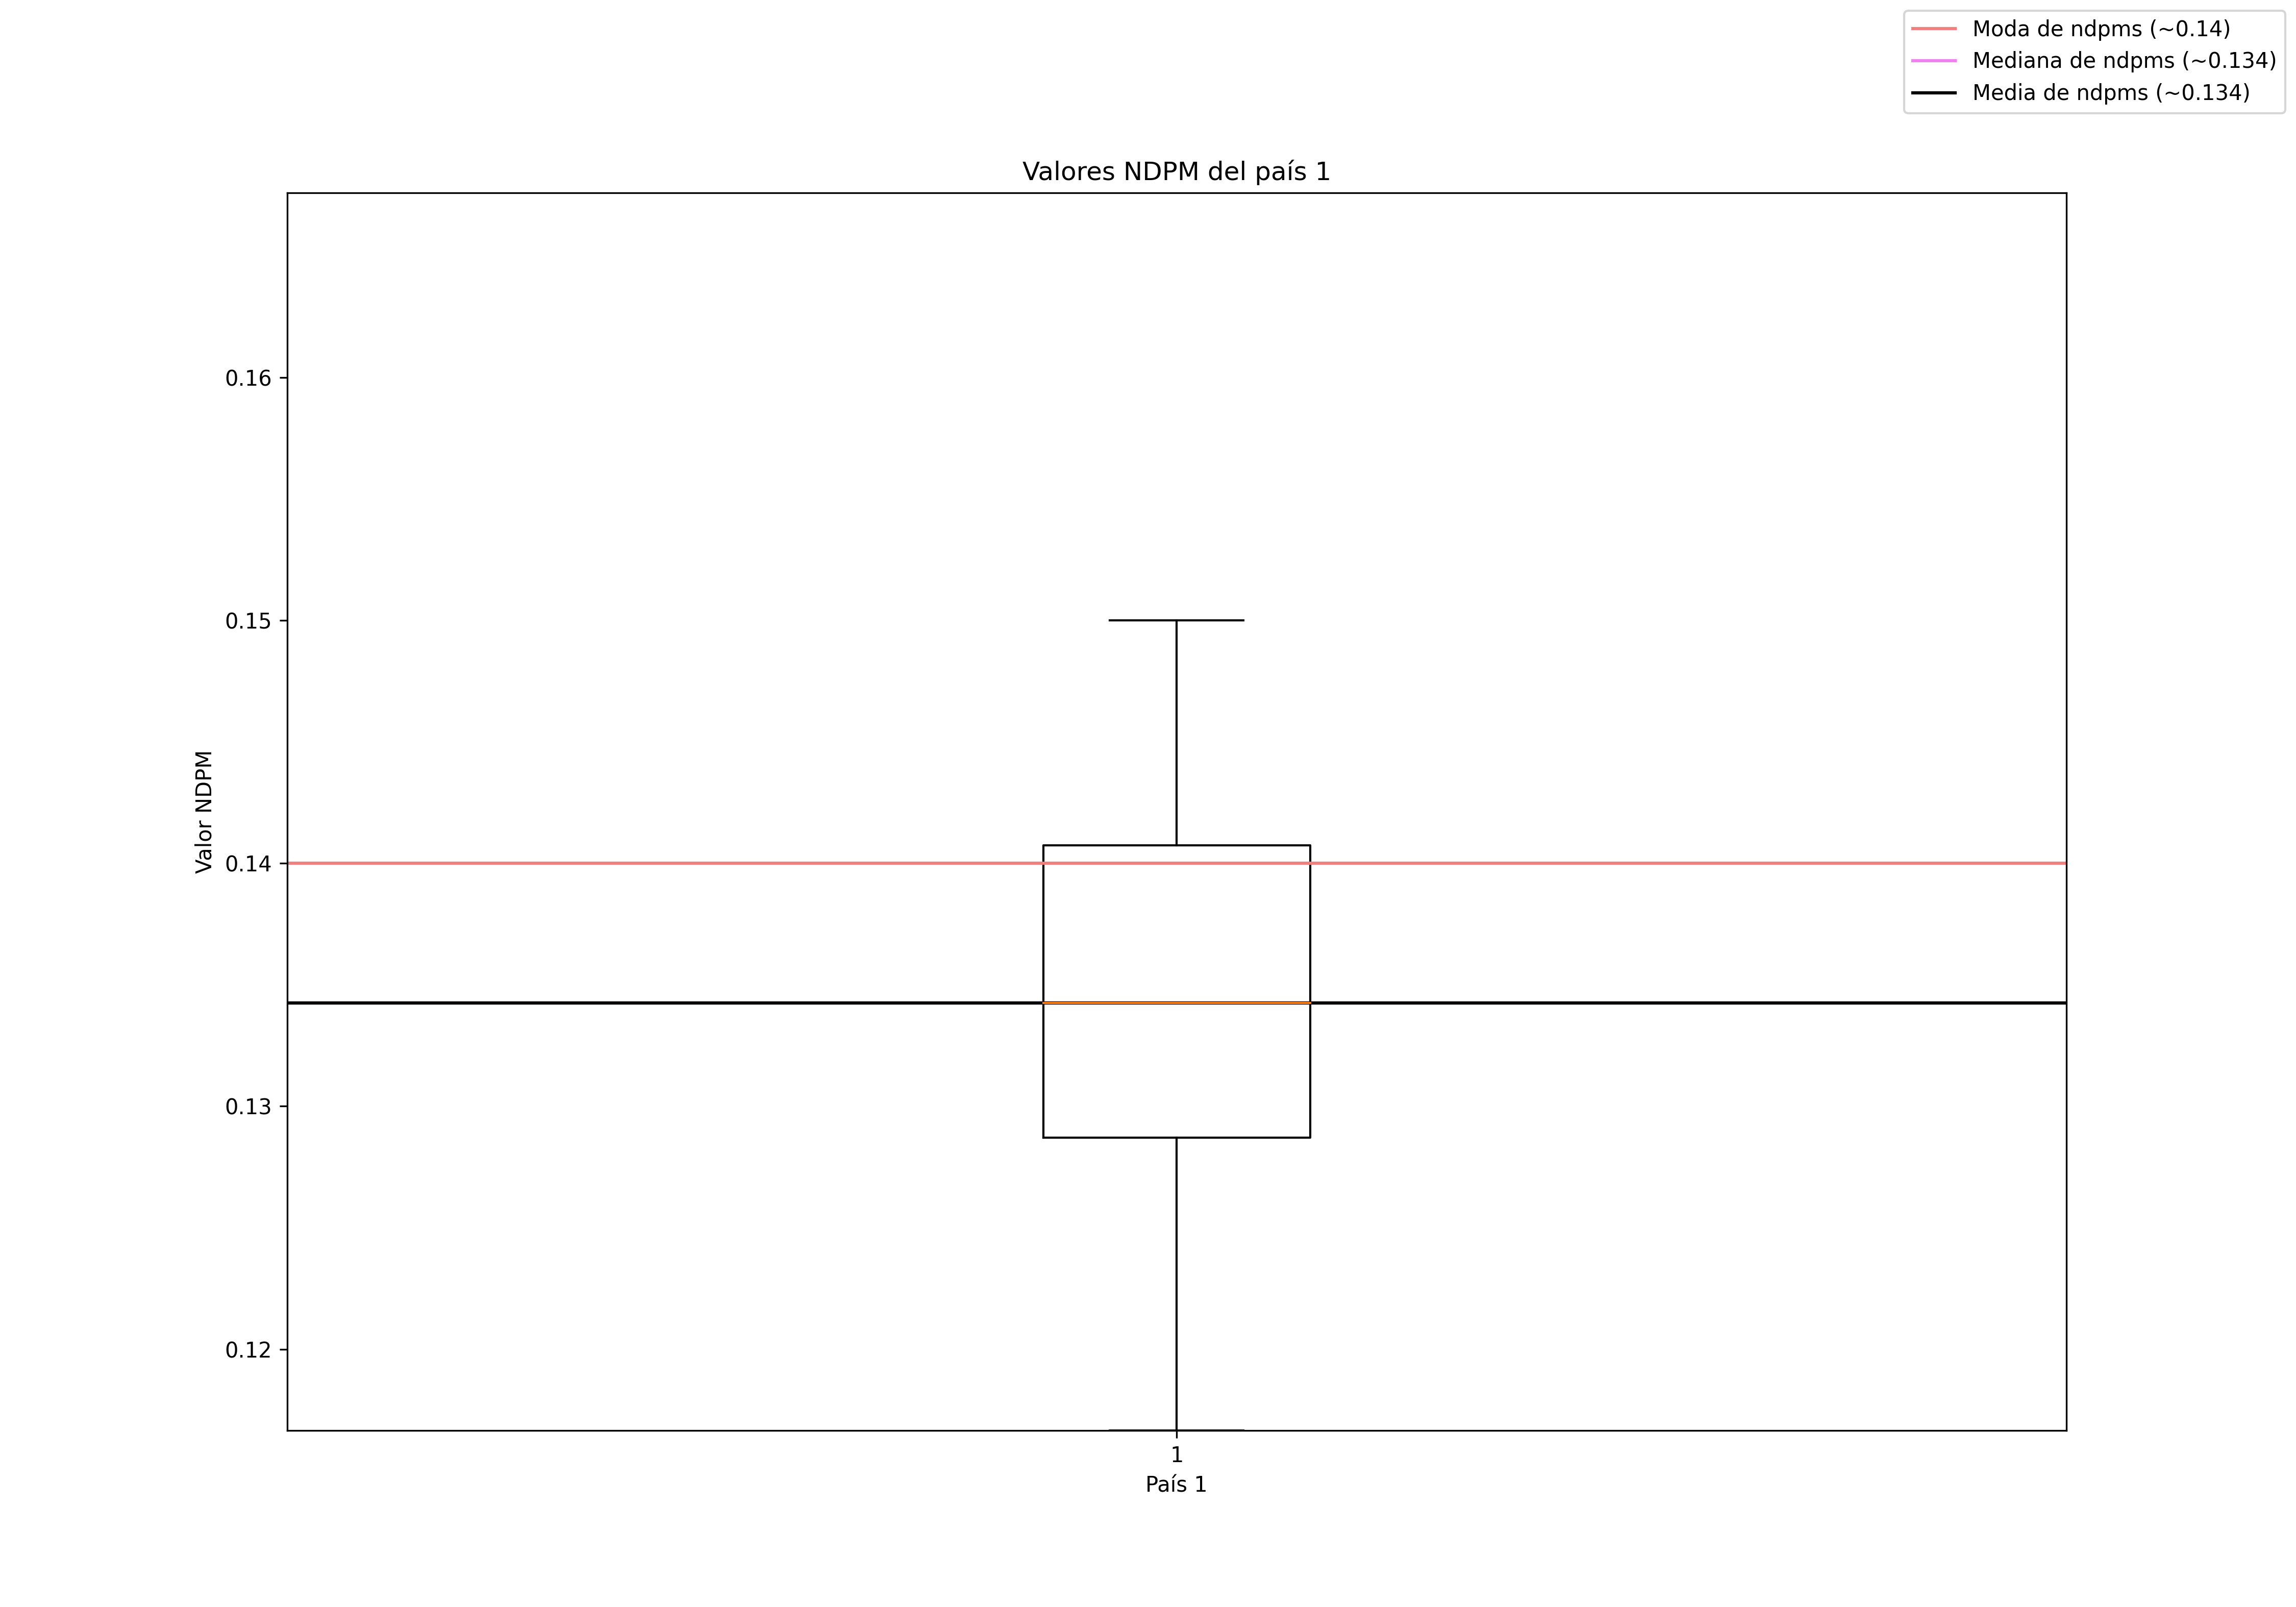
\includegraphics[width=0.5\textheight]
        {Figuras/Reports/PI_1_W0_LOC_CAJAS.png}}
        \quad
    \subfloat[Reentrenado con \textit{W$_c$ $=0$}]
        {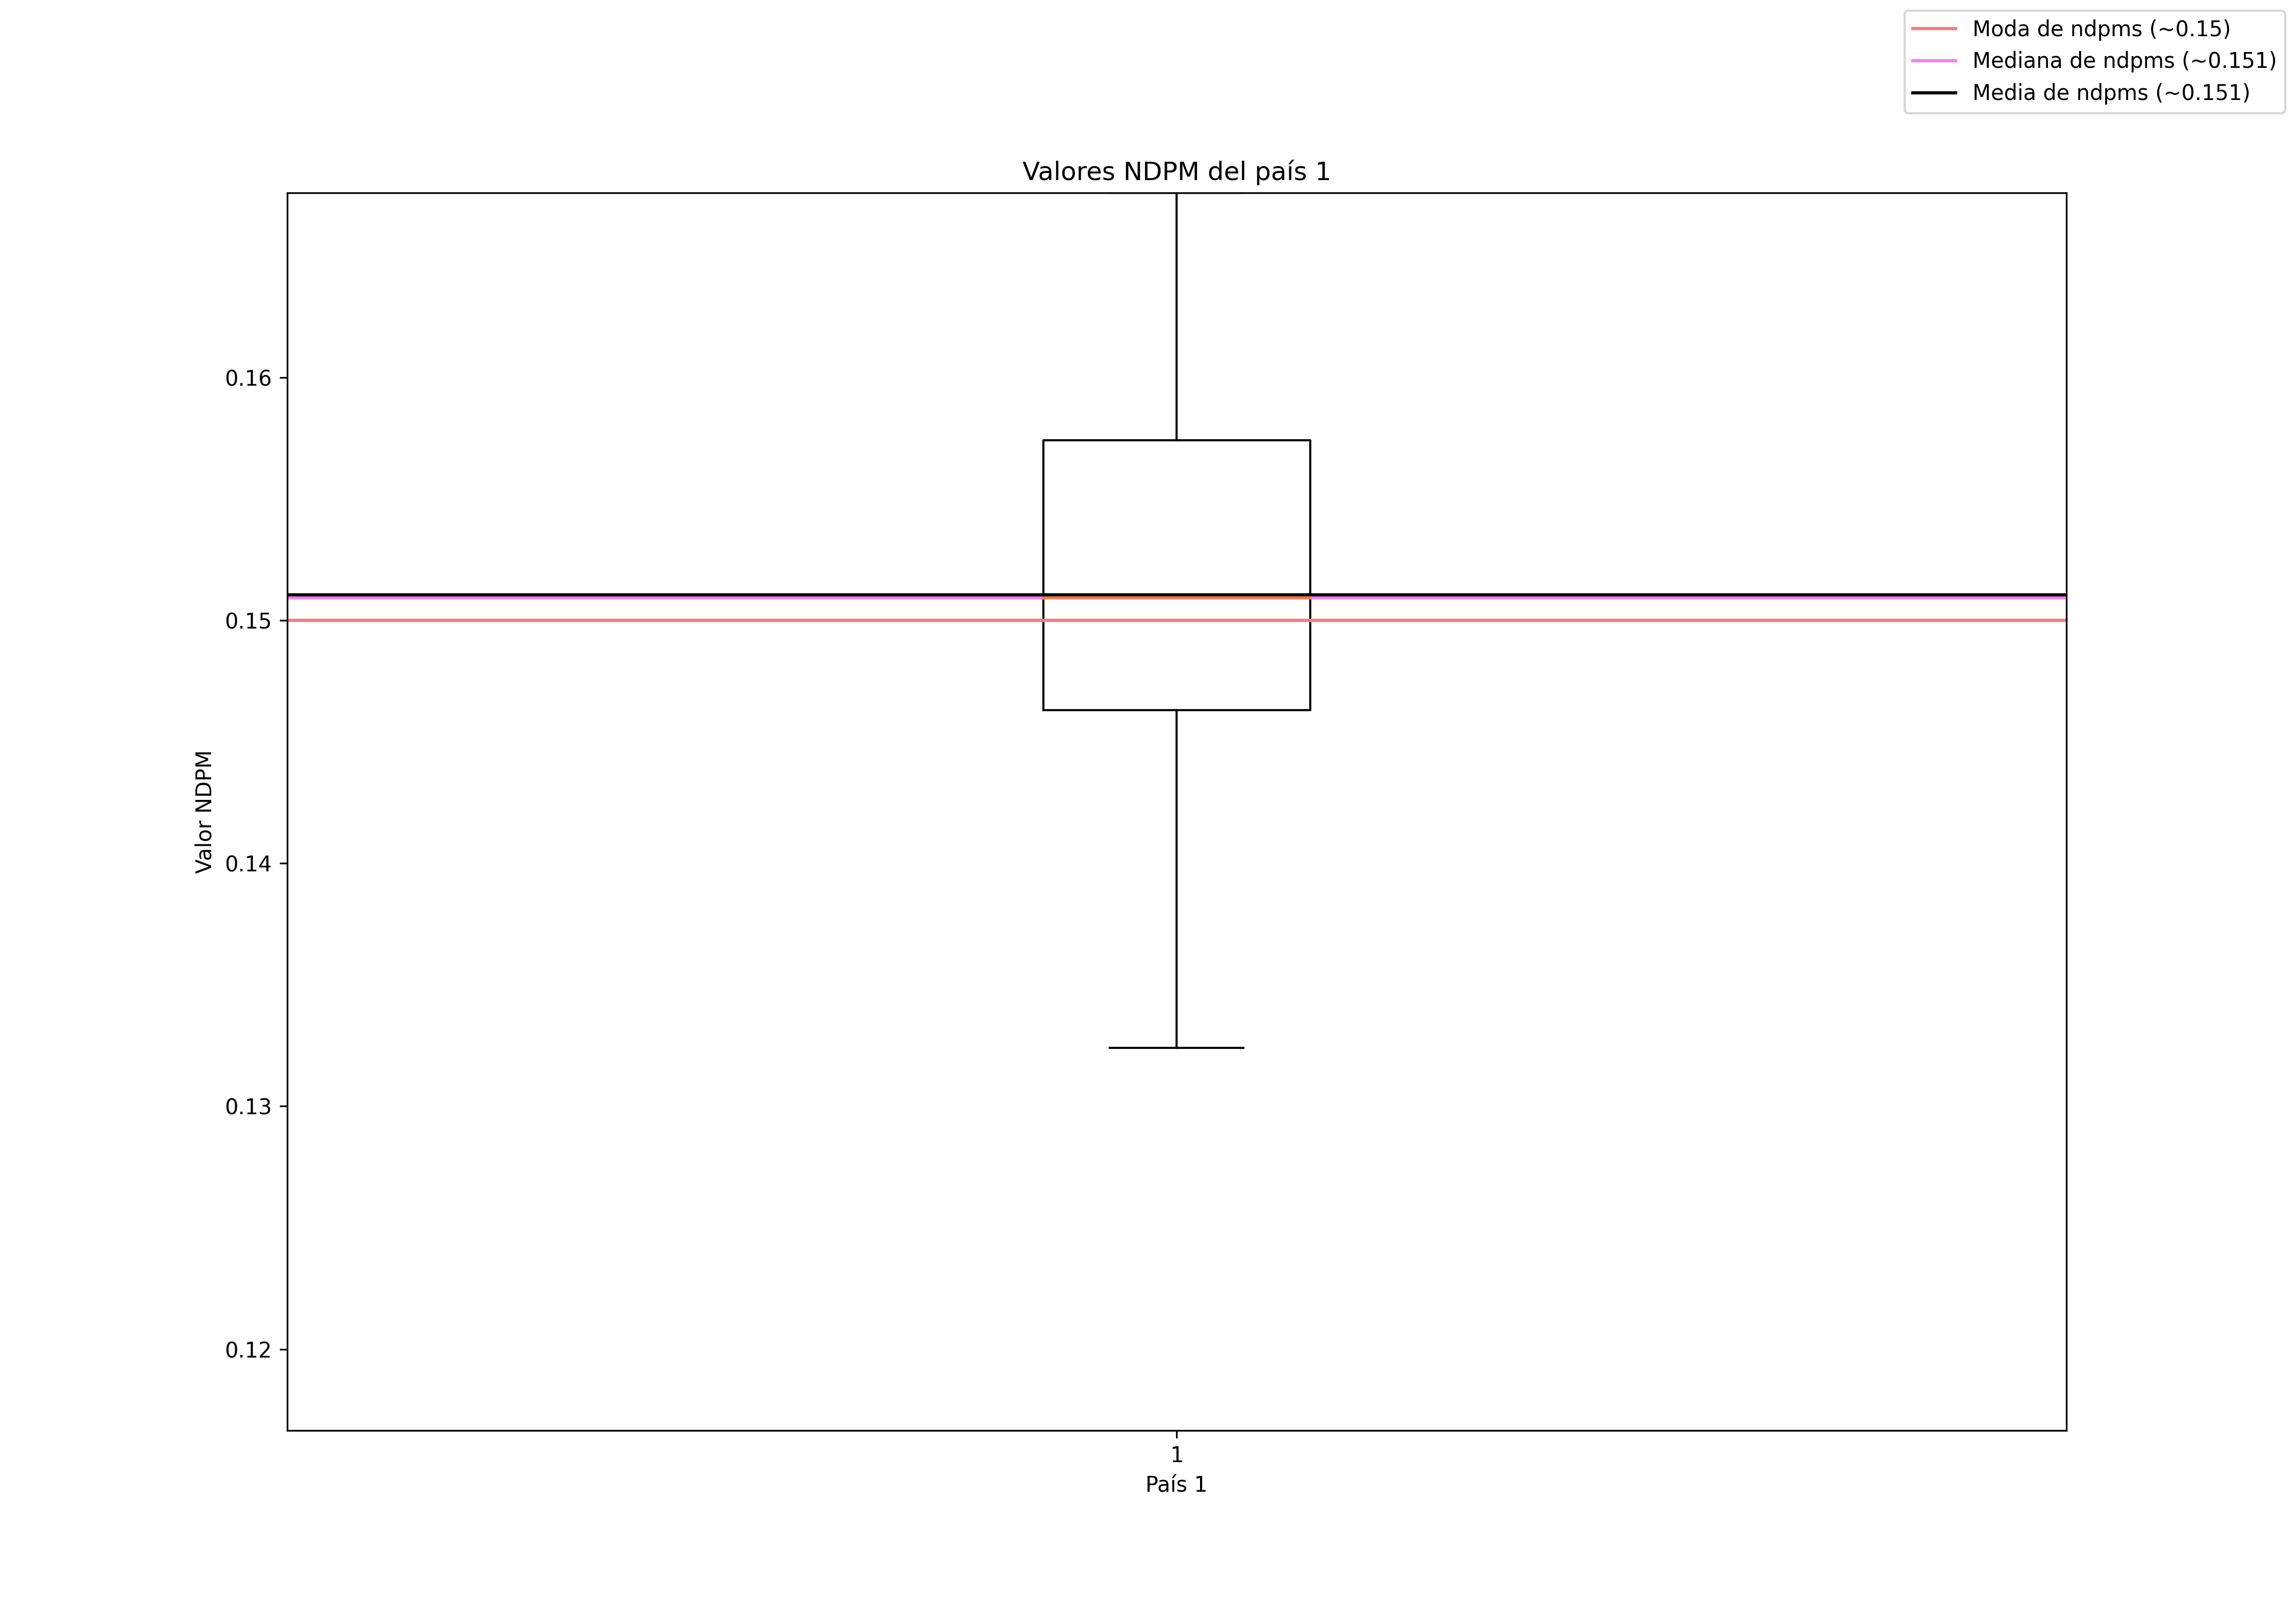
\includegraphics[width=0.5\textheight]
        {Figuras/Reports/PI_1_W0_EXT_CAJAS.png}}
    \subfloat[Reentrenado con \textit{W$_c$ $=1$}]{
        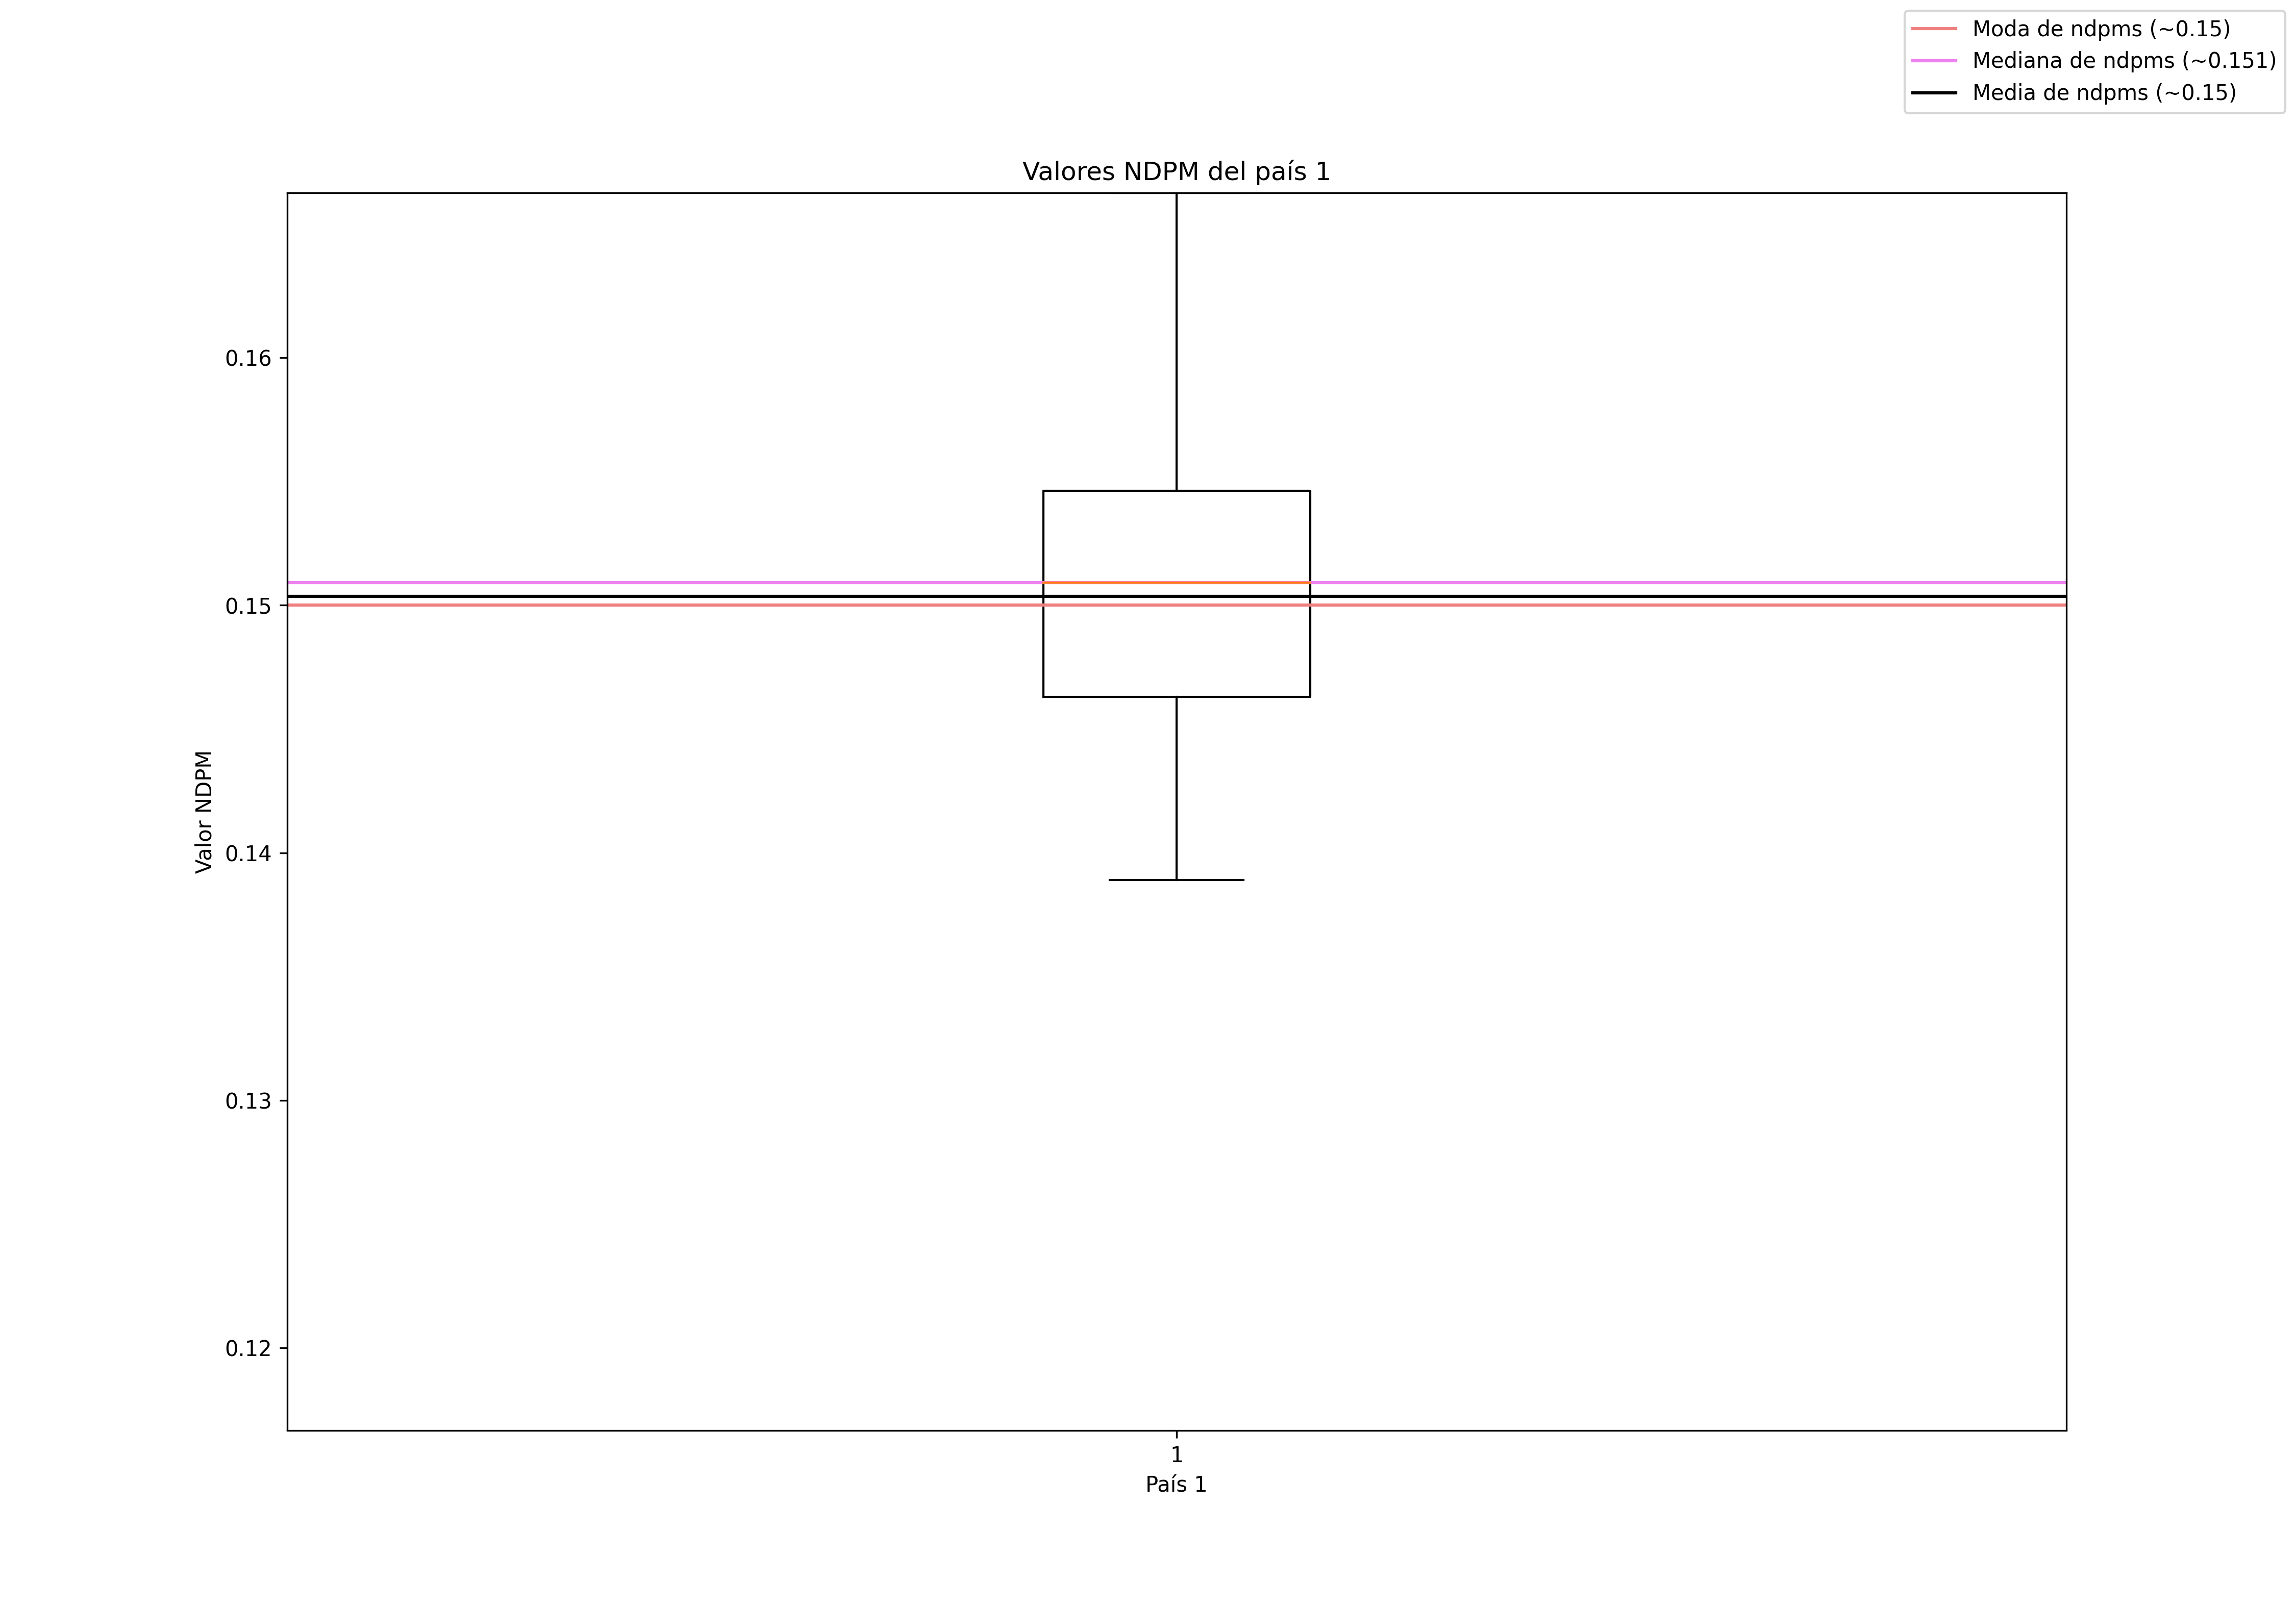
\includegraphics[width=0.5\textheight]
        {Figuras/Reports/PI_1_W1_EXT_CAJAS.png}}
    \caption{Diagramas de cajas y bigotes de los valores NDPM del participante 1\label{fig:PI1_CAJAS}}
\end{sidewaysfigure}
\clearpage
\begin{sidewaysfigure}
    \centering
    \subfloat[Modelo original]
        {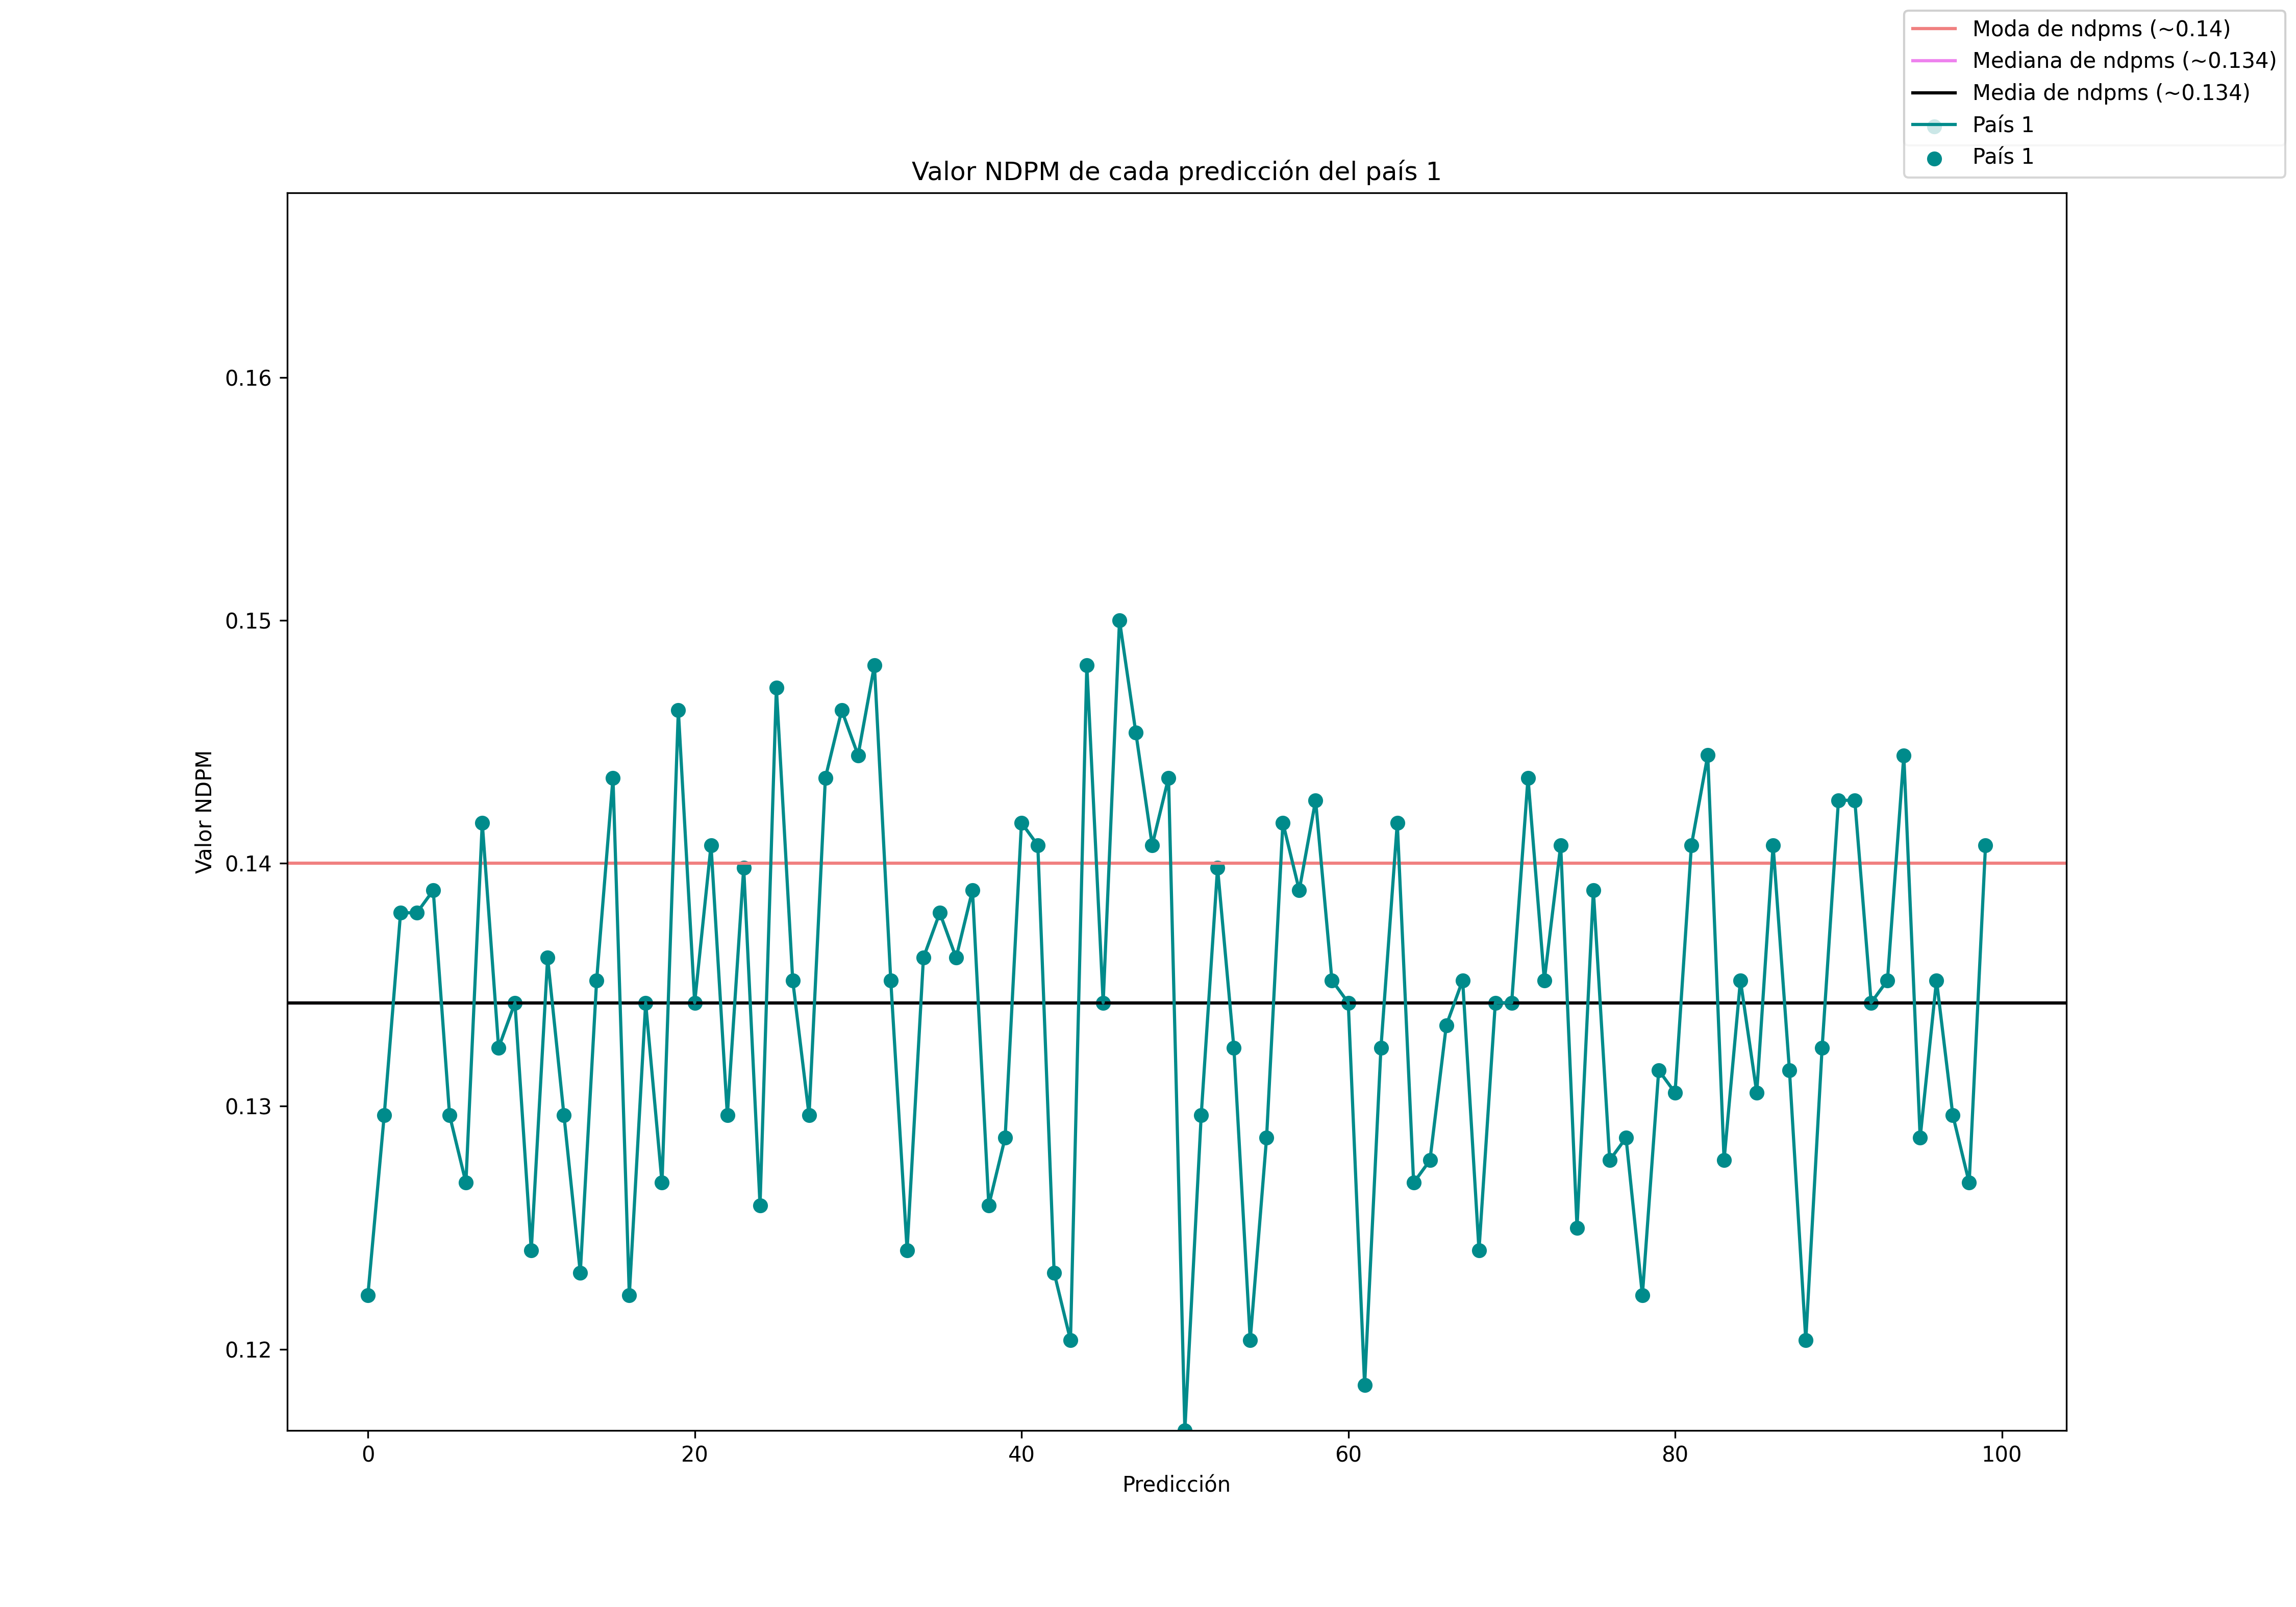
\includegraphics[width=0.5\textheight]
        {Figuras/Reports/PI_1_W0_LOC_DISP.png}}
        \quad
    \subfloat[Reentrenado con \textit{W$_c$ $=0$}]
        {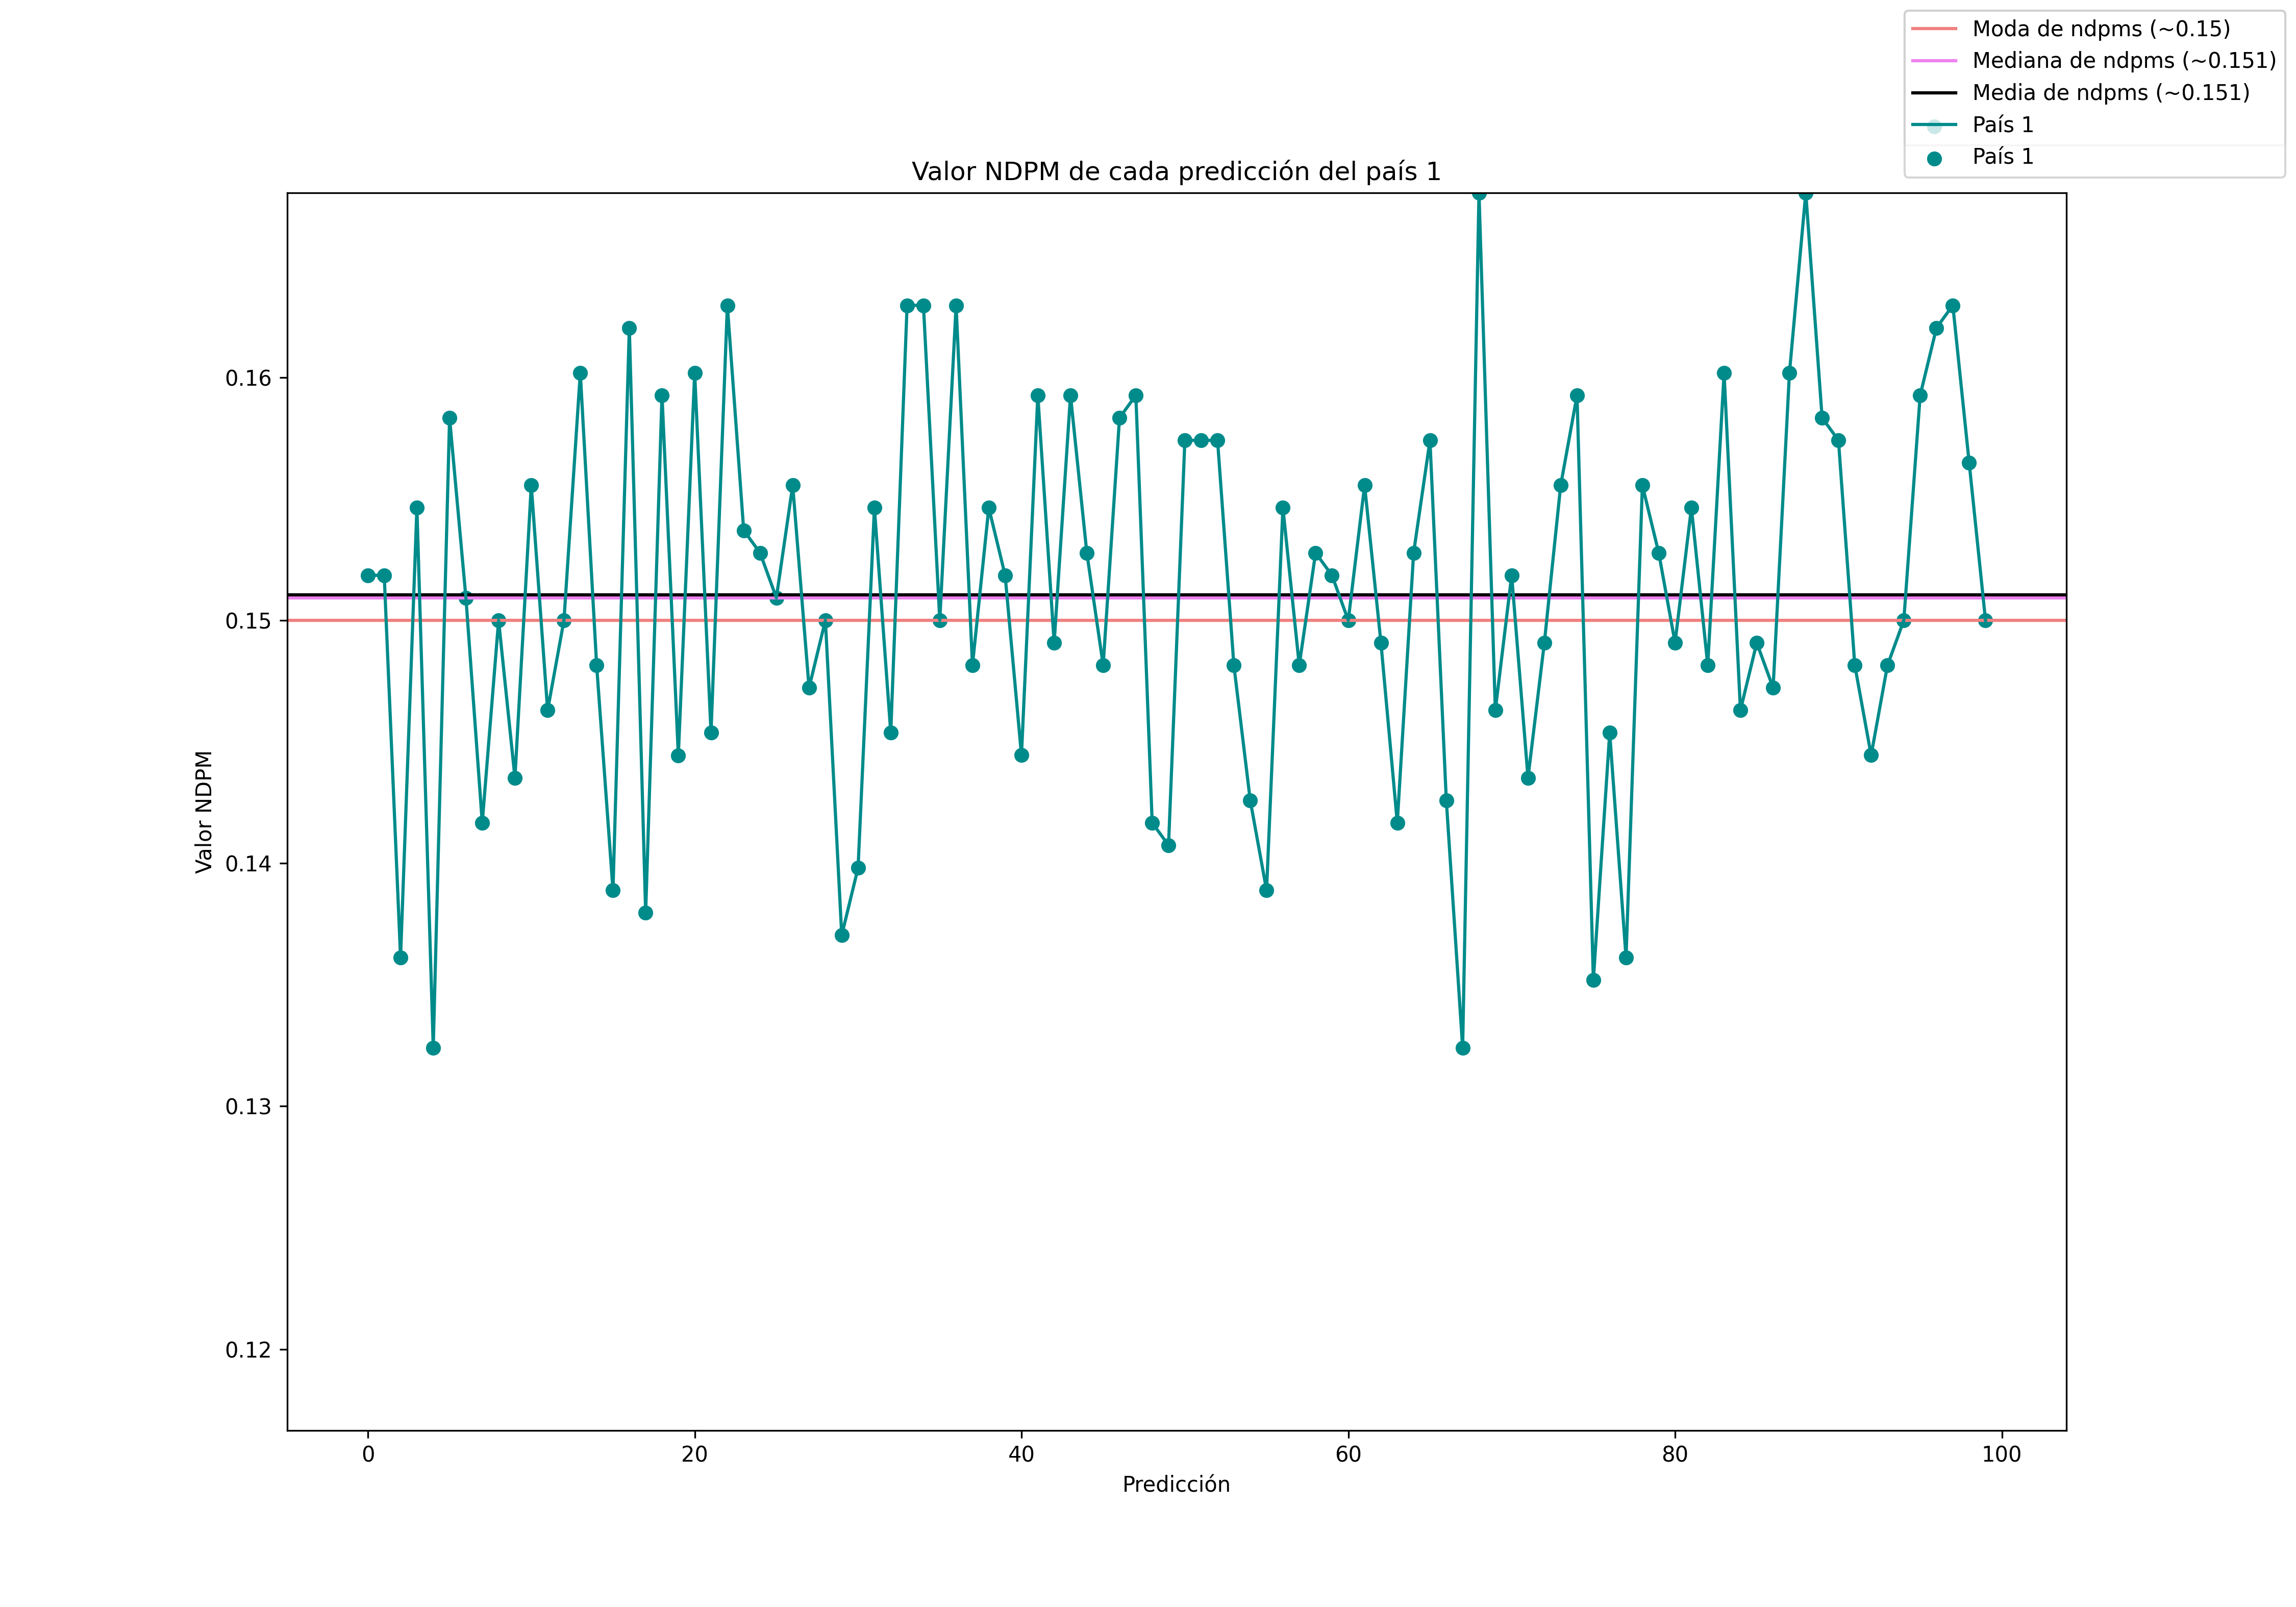
\includegraphics[width=0.5\textheight]
        {Figuras/Reports/PI_1_W0_EXT_DISP.png}}
    \subfloat[Reentrenado con \textit{W$_c$ $=1$}]{
        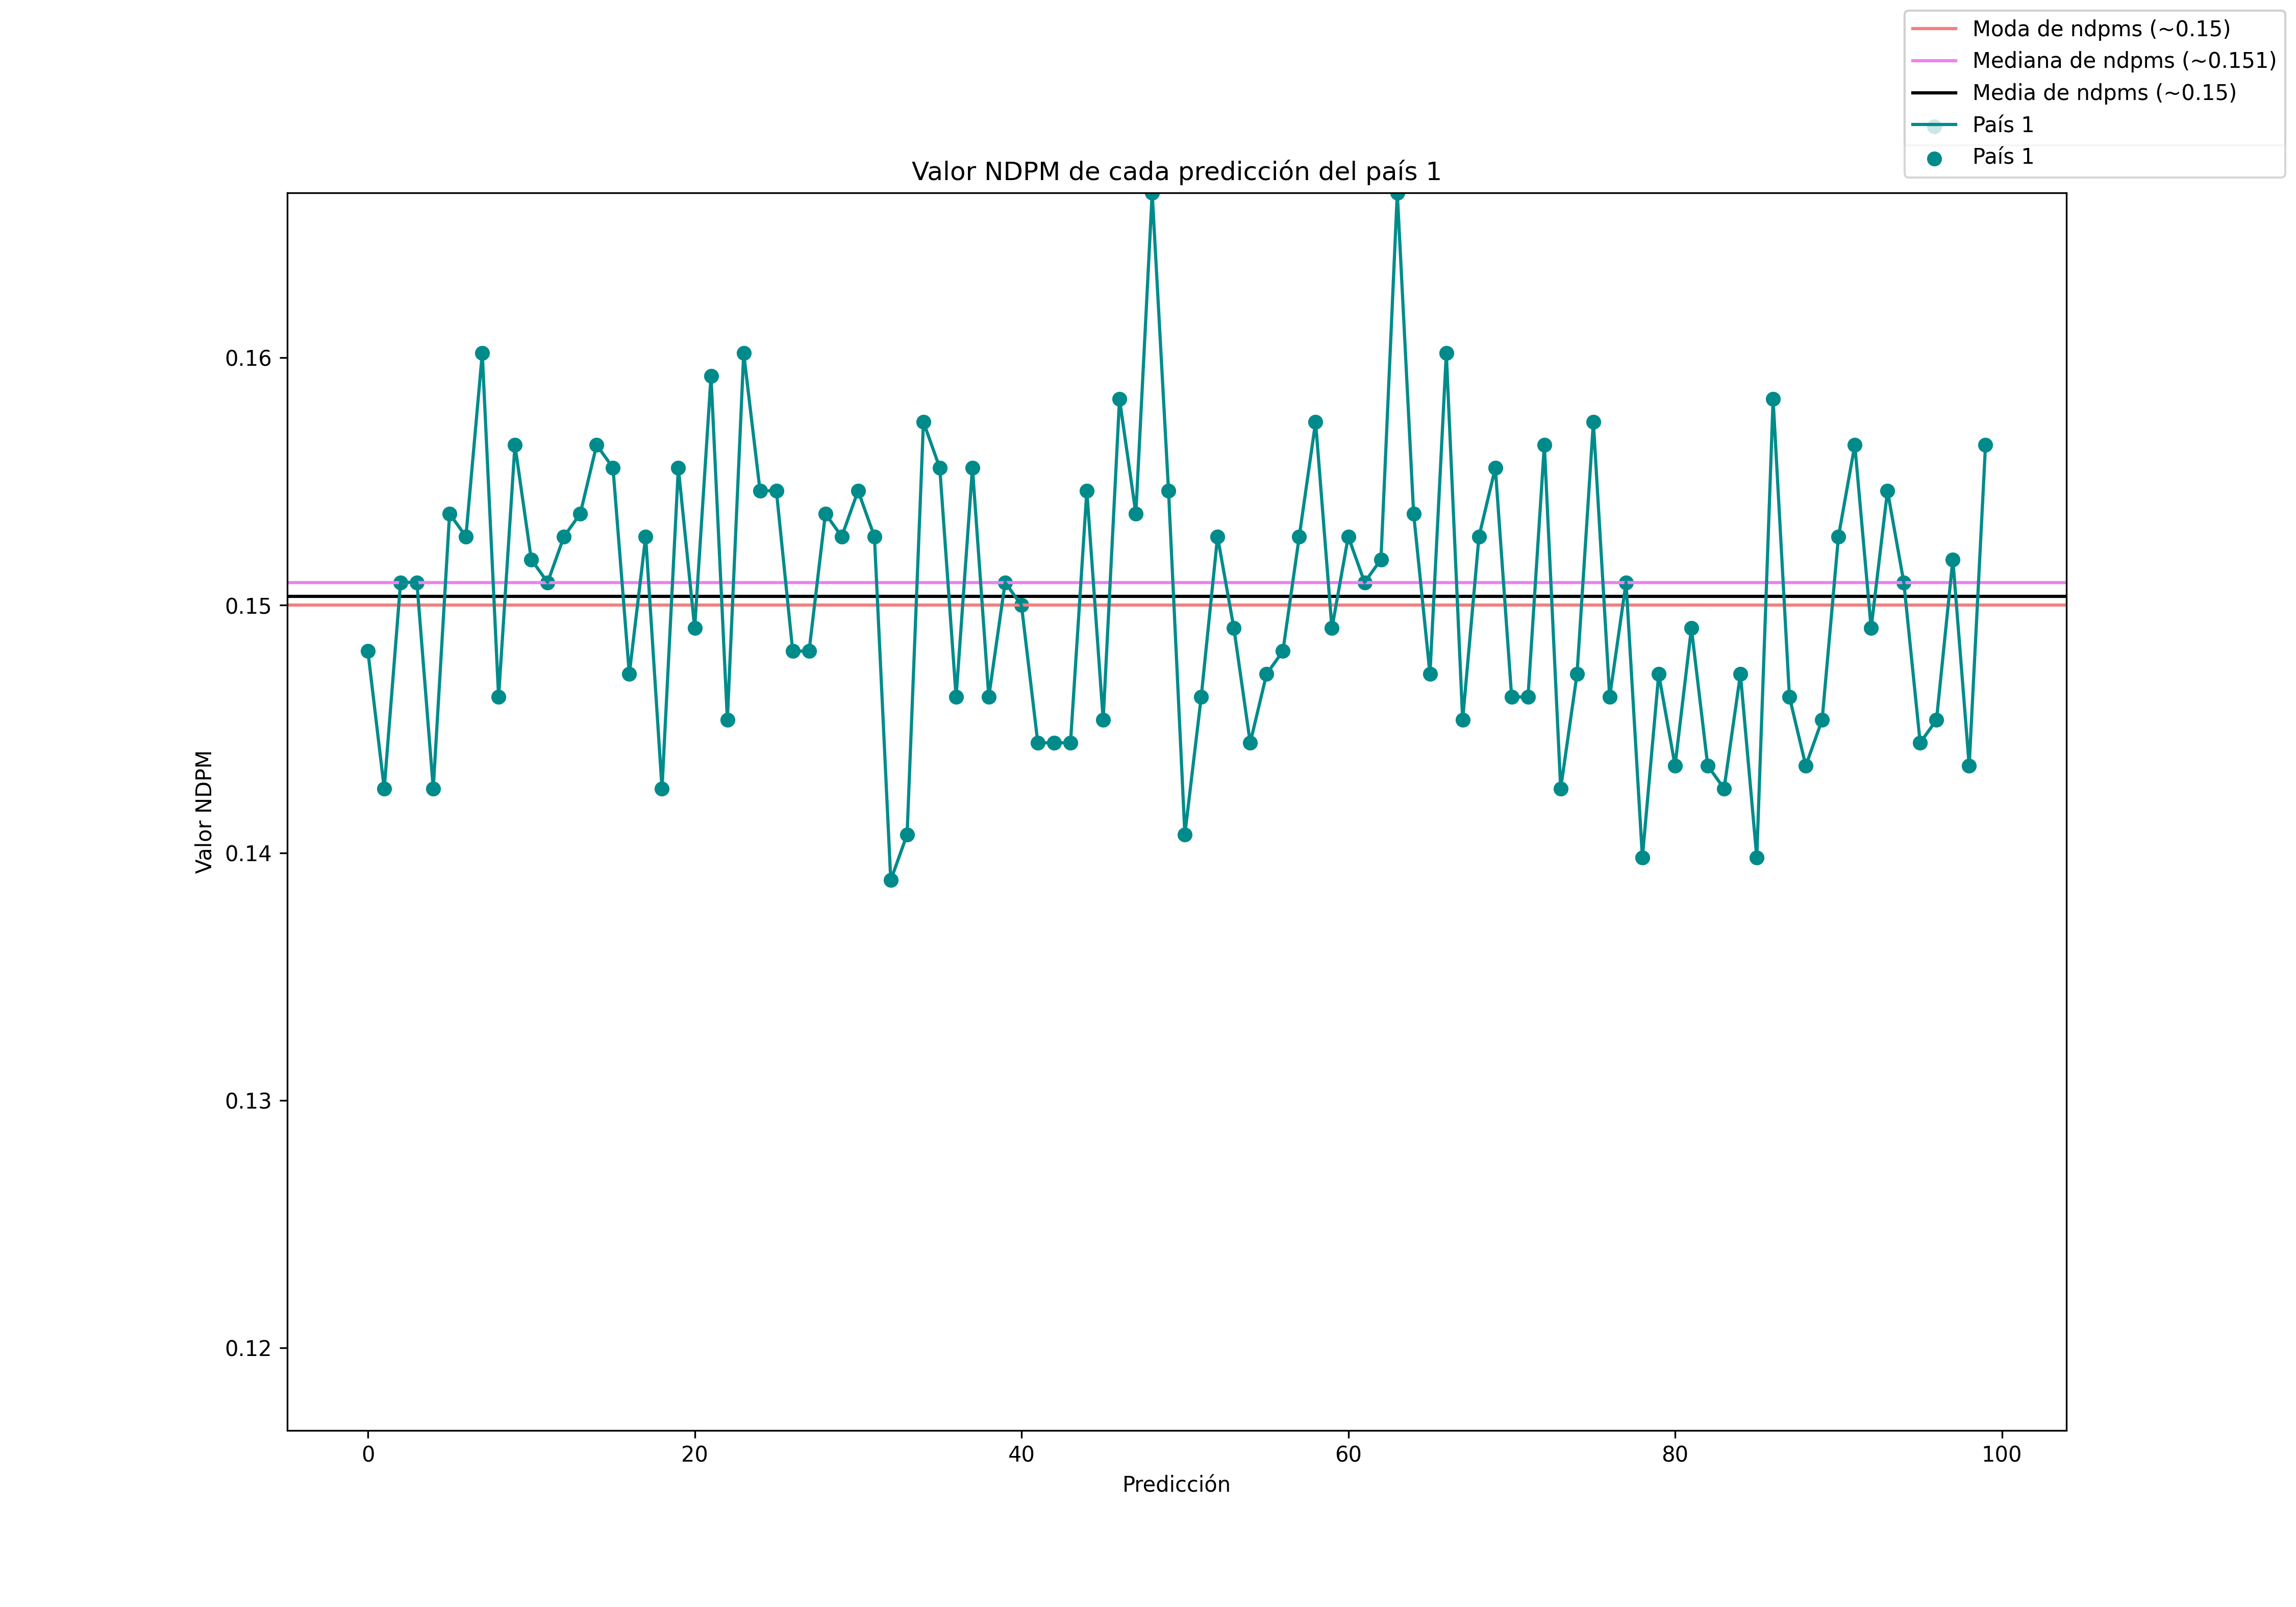
\includegraphics[width=0.5\textheight]
        {Figuras/Reports/PI_1_W1_EXT_DISP.png}}
    \caption{Gráfico de los valores NDPM del participante 1\label{fig:PI1_DISP}}
\end{sidewaysfigure}
\clearpage

\begin{sidewaysfigure}
    \centering
    \subfloat[Modelo original]
        {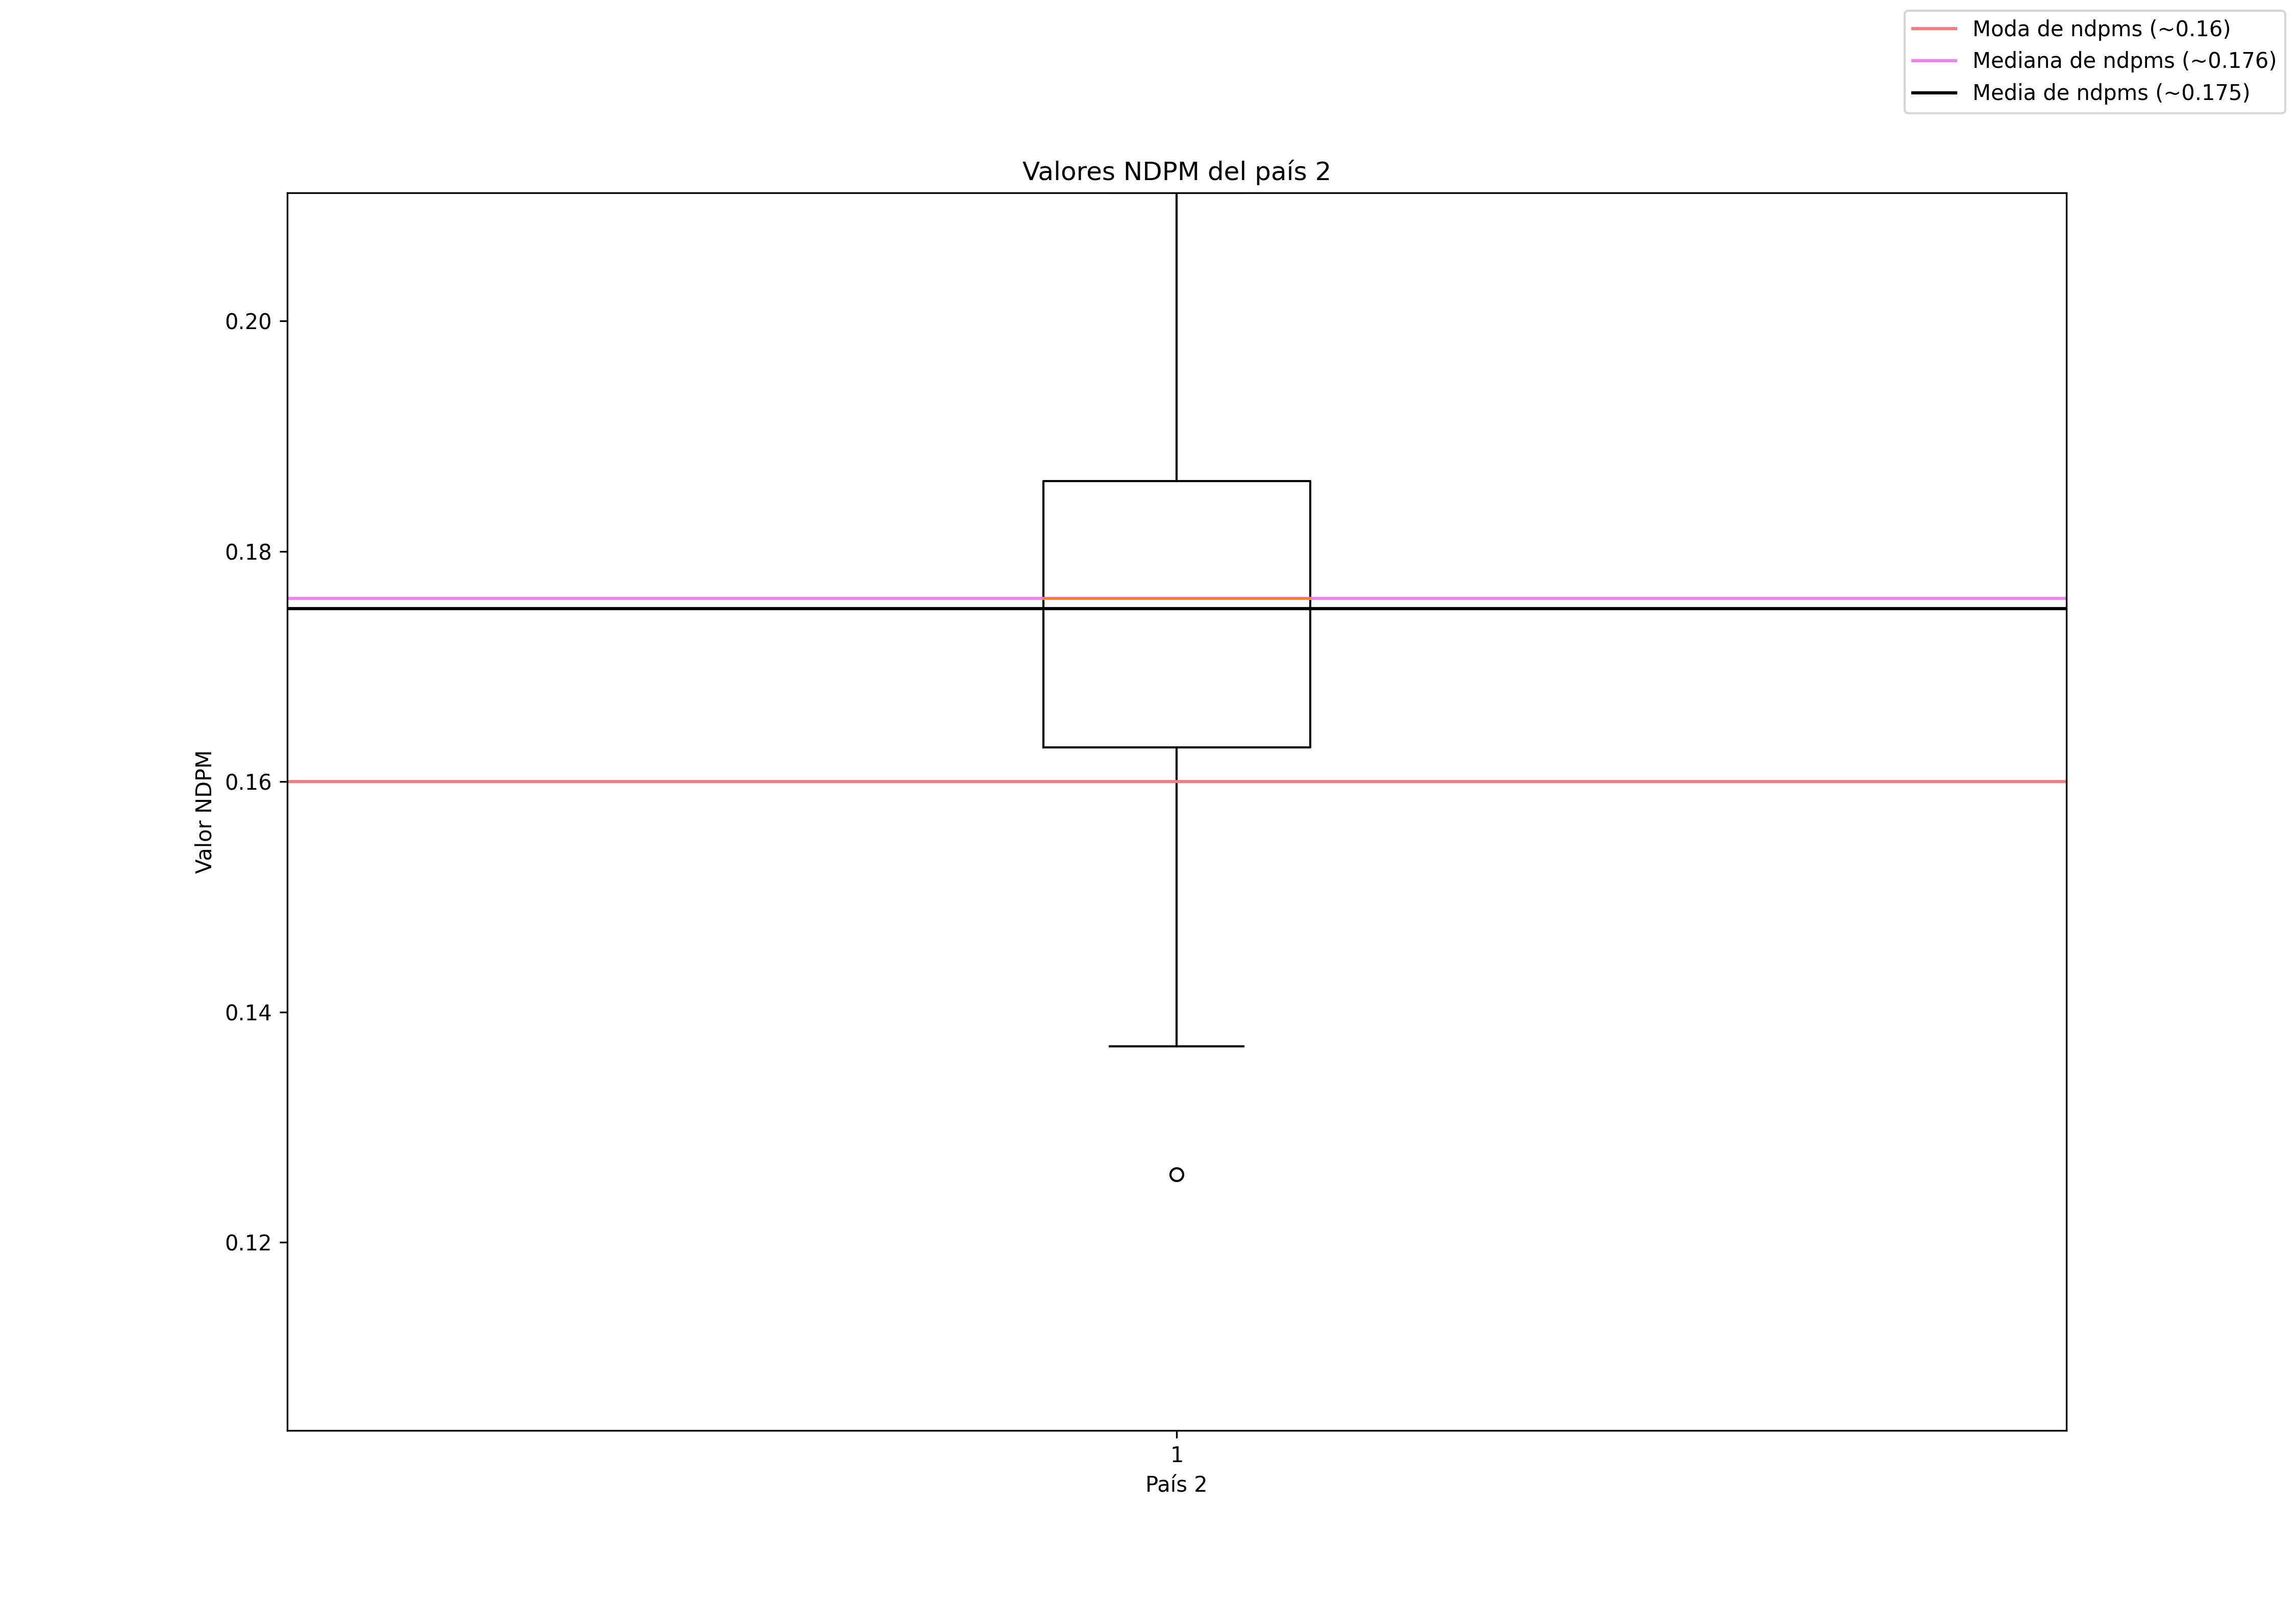
\includegraphics[width=0.5\textheight]
        {Figuras/Reports/PI_2_W0_LOC_CAJAS.png}}
        \quad
    \subfloat[Reentrenado con \textit{W$_c$ $=0$}]
        {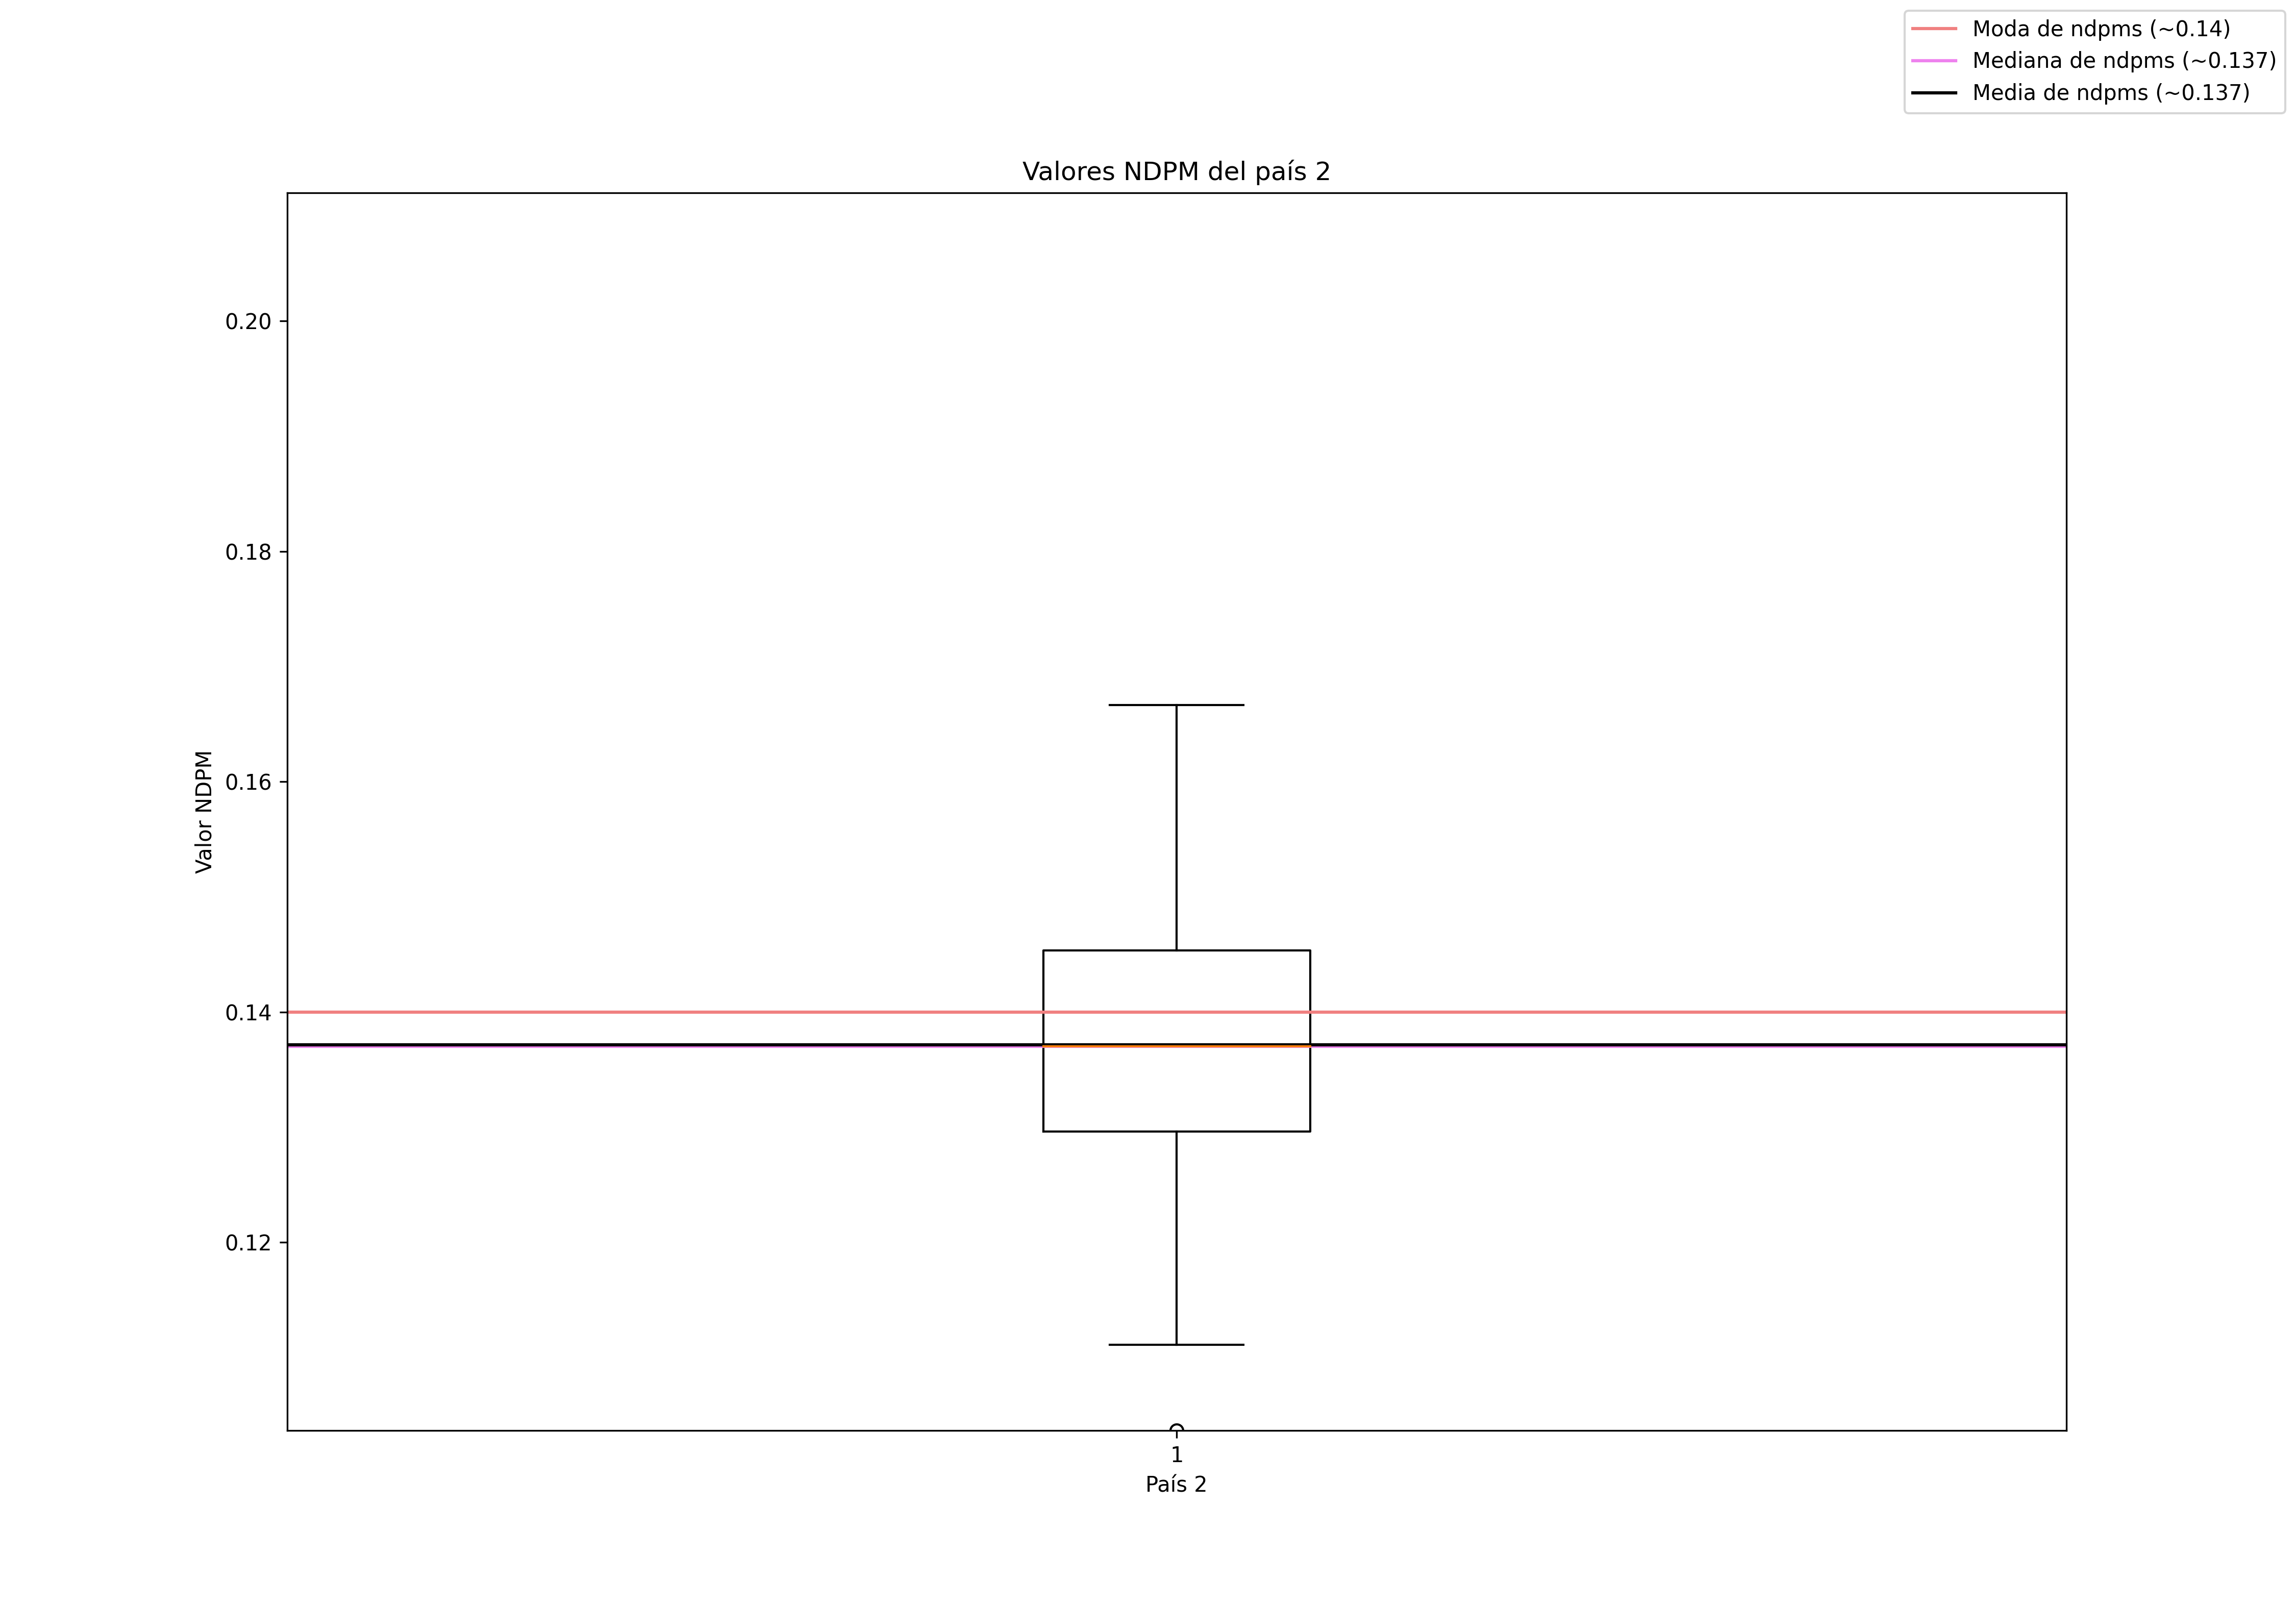
\includegraphics[width=0.5\textheight]
        {Figuras/Reports/PI_2_W0_EXT_CAJAS.png}}
    \subfloat[Reentrenado con \textit{W$_c$ $=1$}]{
        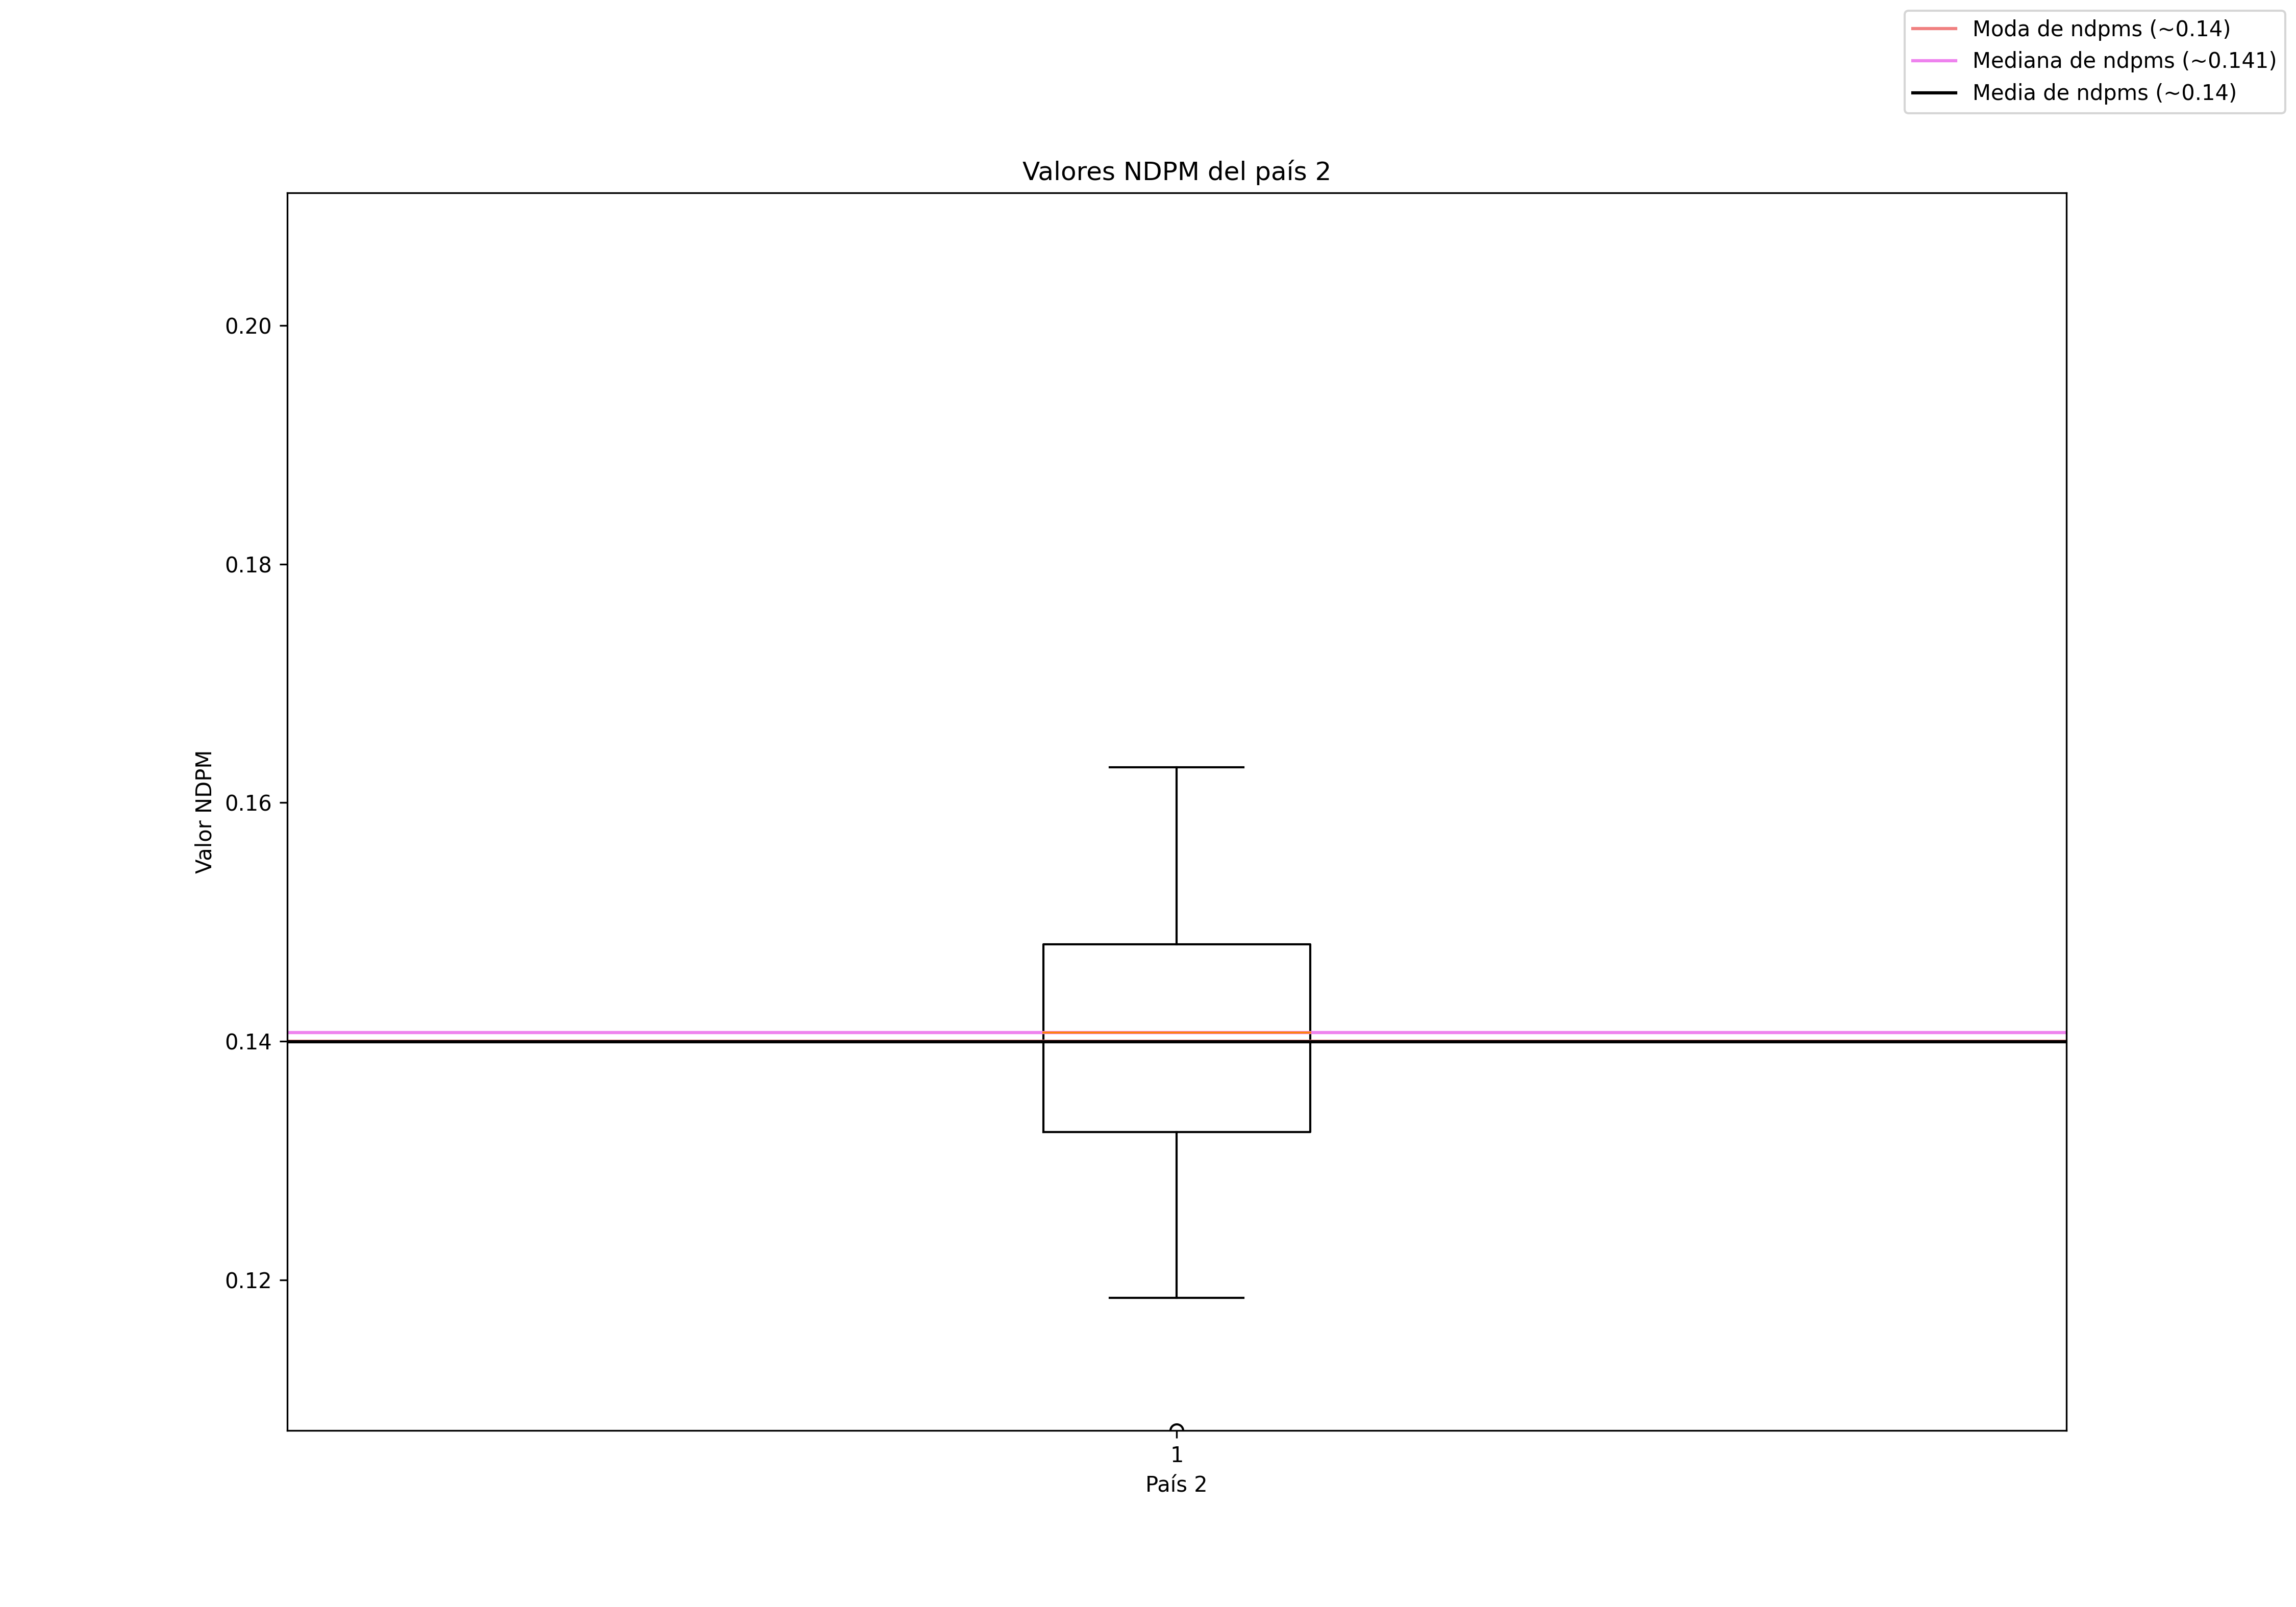
\includegraphics[width=0.5\textheight]
        {Figuras/Reports/PI_2_W1_EXT_CAJAS.png}}
    \caption{Diagramas de cajas y bigotes de los valores NDPM del participante 2\label{fig:PI2_CAJAS}}
\end{sidewaysfigure}
\clearpage
\begin{sidewaysfigure}
    \centering
    \subfloat[Modelo original]
        {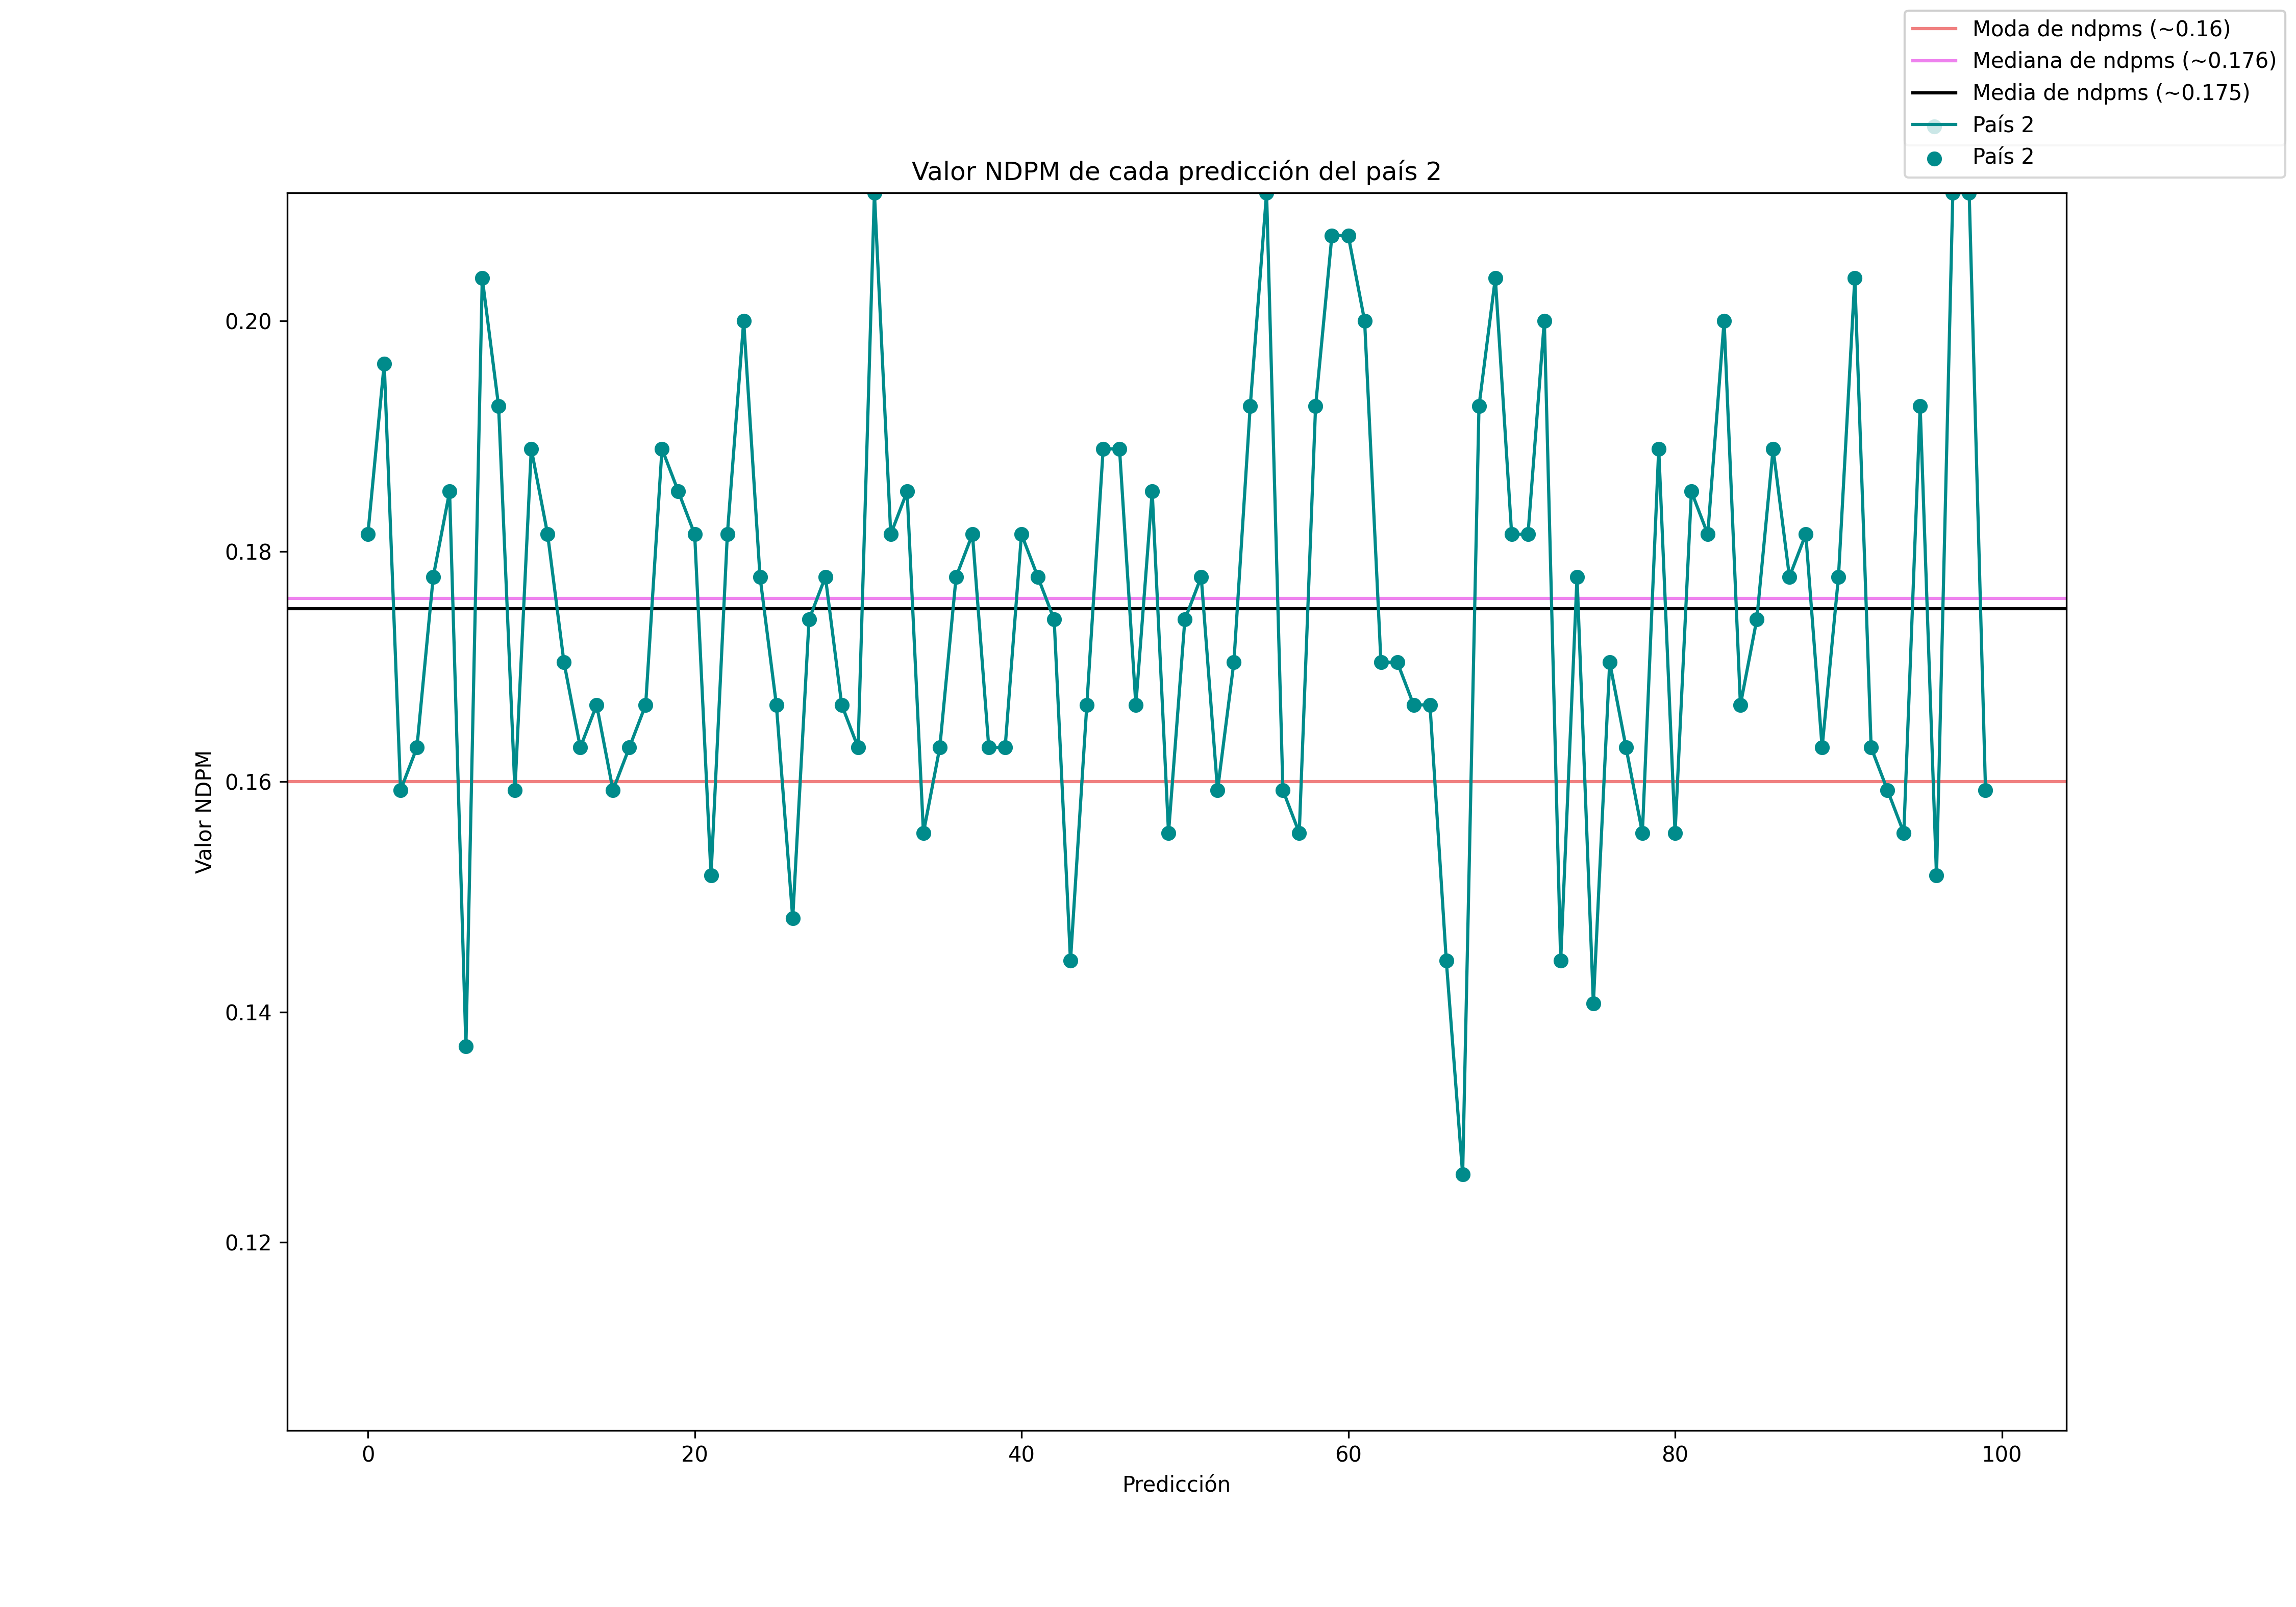
\includegraphics[width=0.5\textheight]
        {Figuras/Reports/PI_2_W0_LOC_DISP.png}}
        \quad
    \subfloat[Reentrenado con \textit{W$_c$ $=0$}]
        {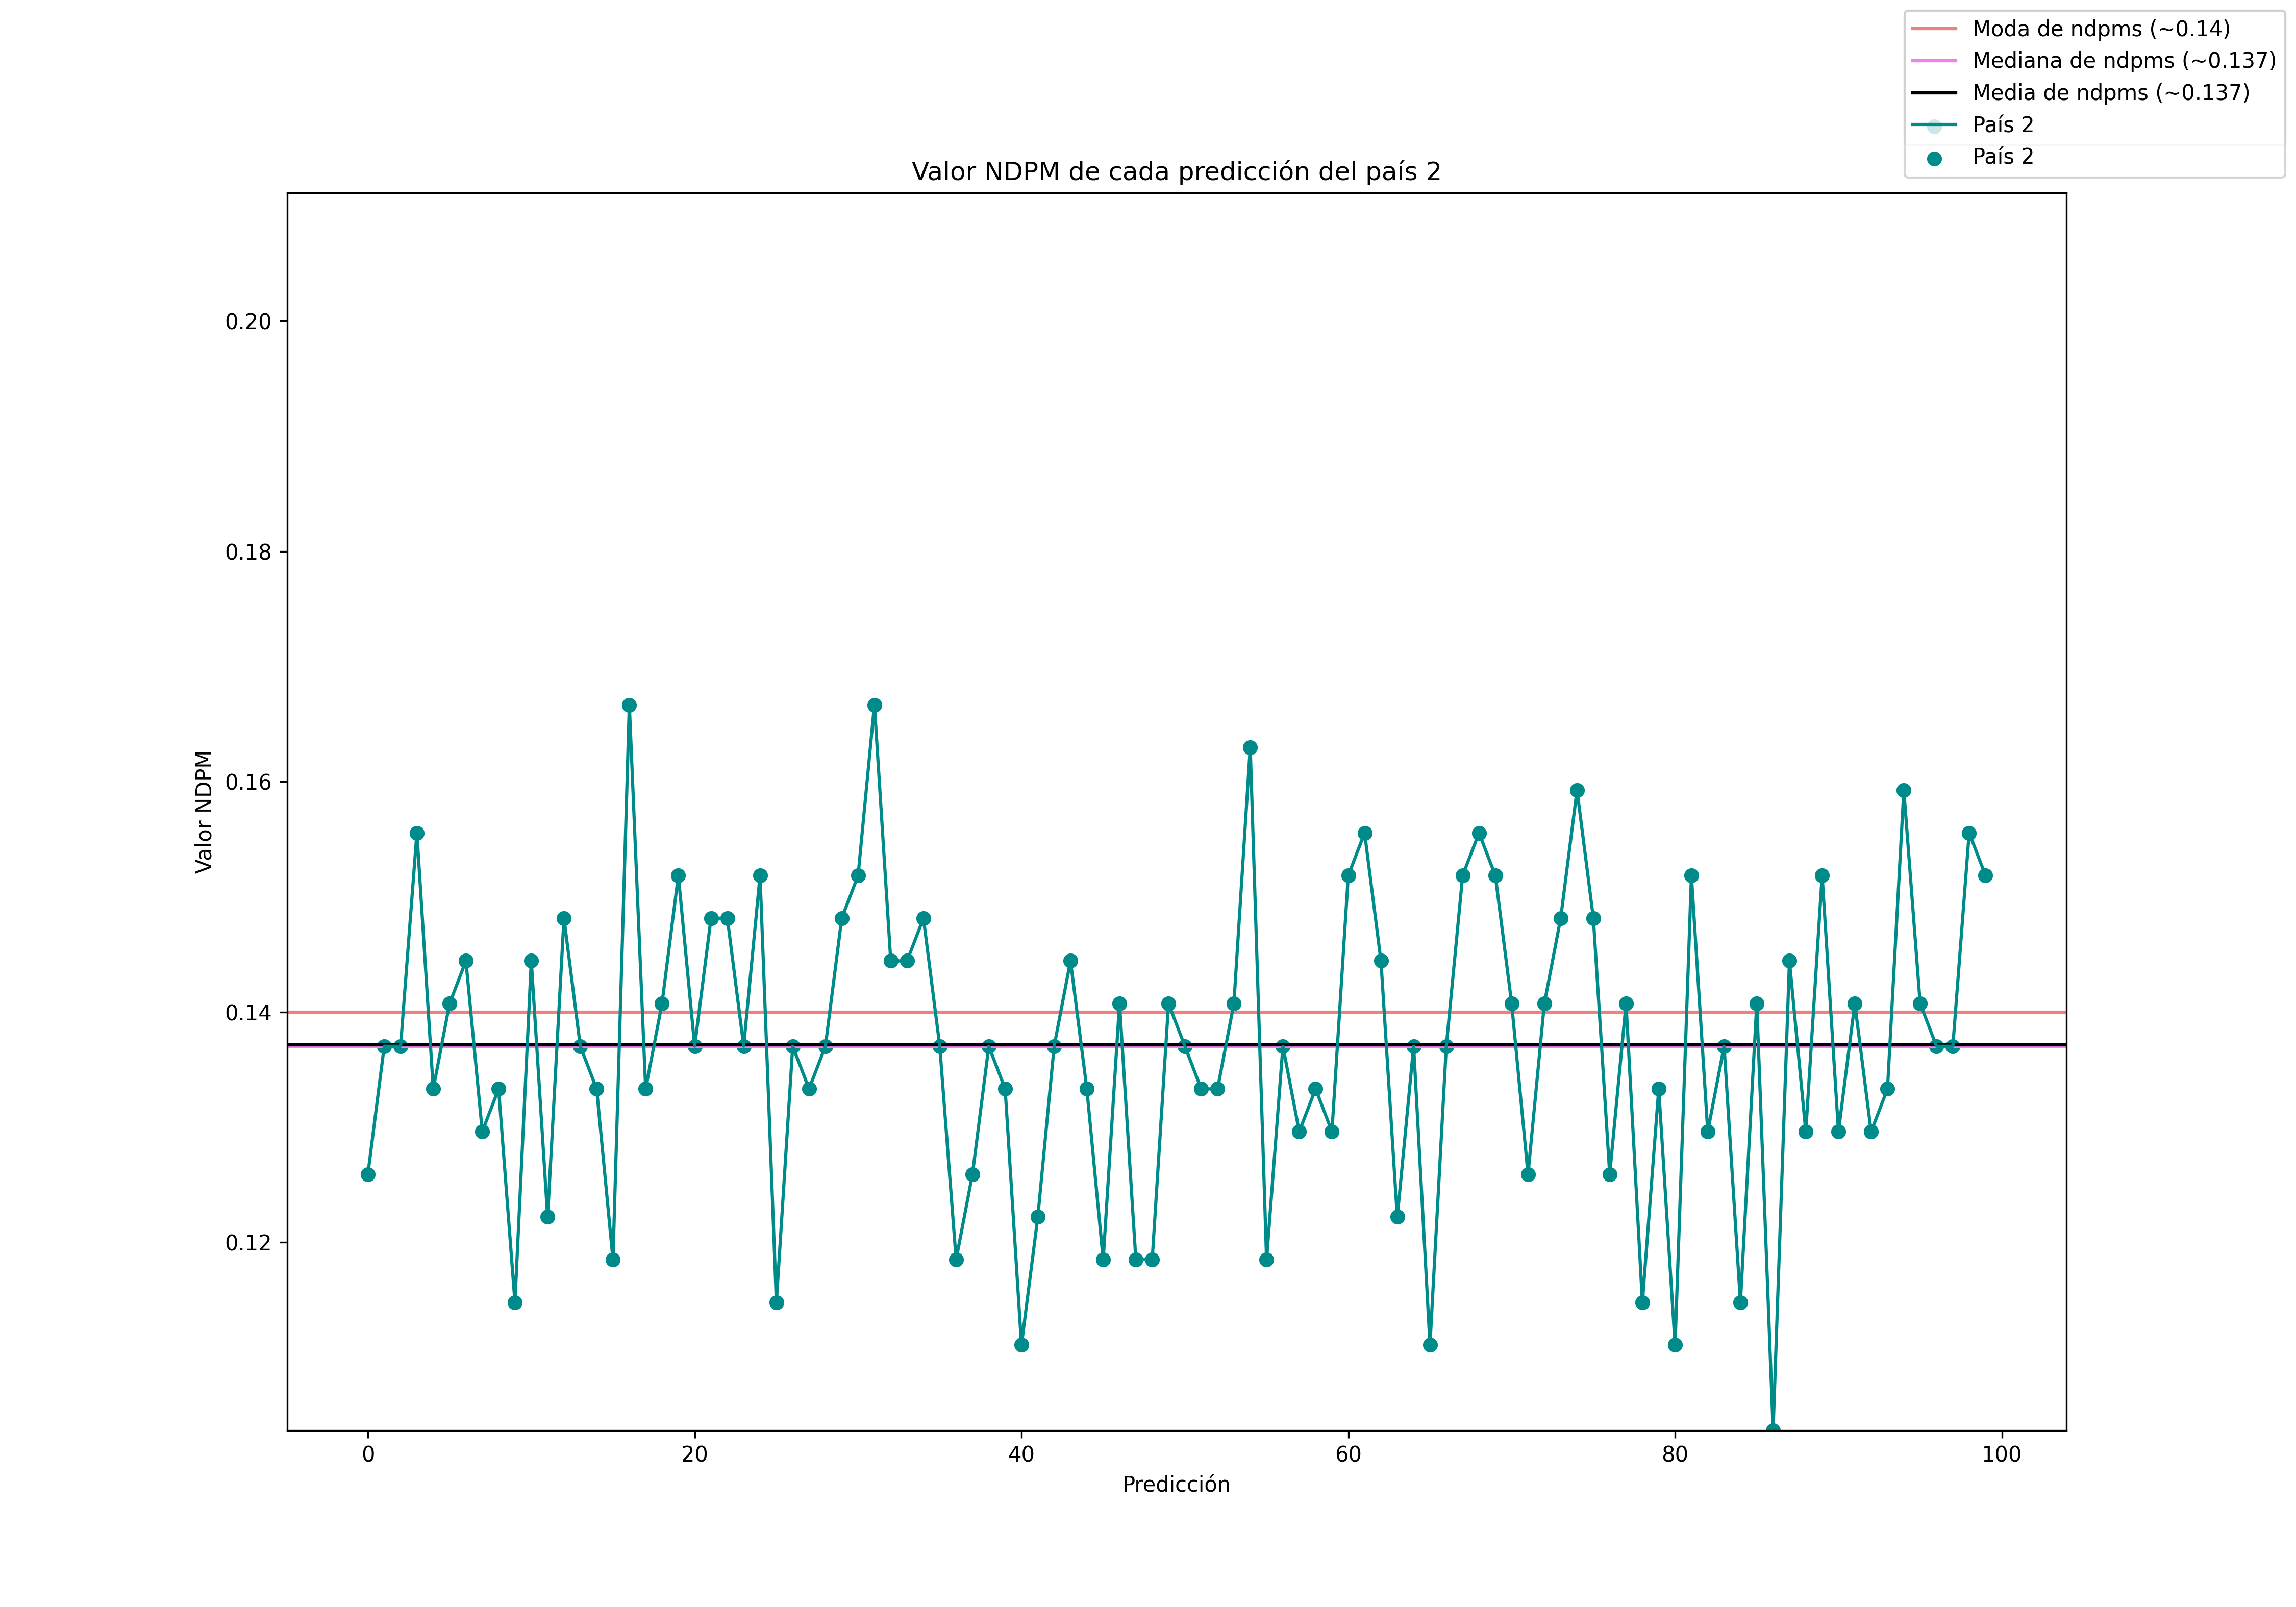
\includegraphics[width=0.5\textheight]
        {Figuras/Reports/PI_2_W0_EXT_DISP.png}}
    \subfloat[Reentrenado con \textit{W$_c$ $=1$}]{
        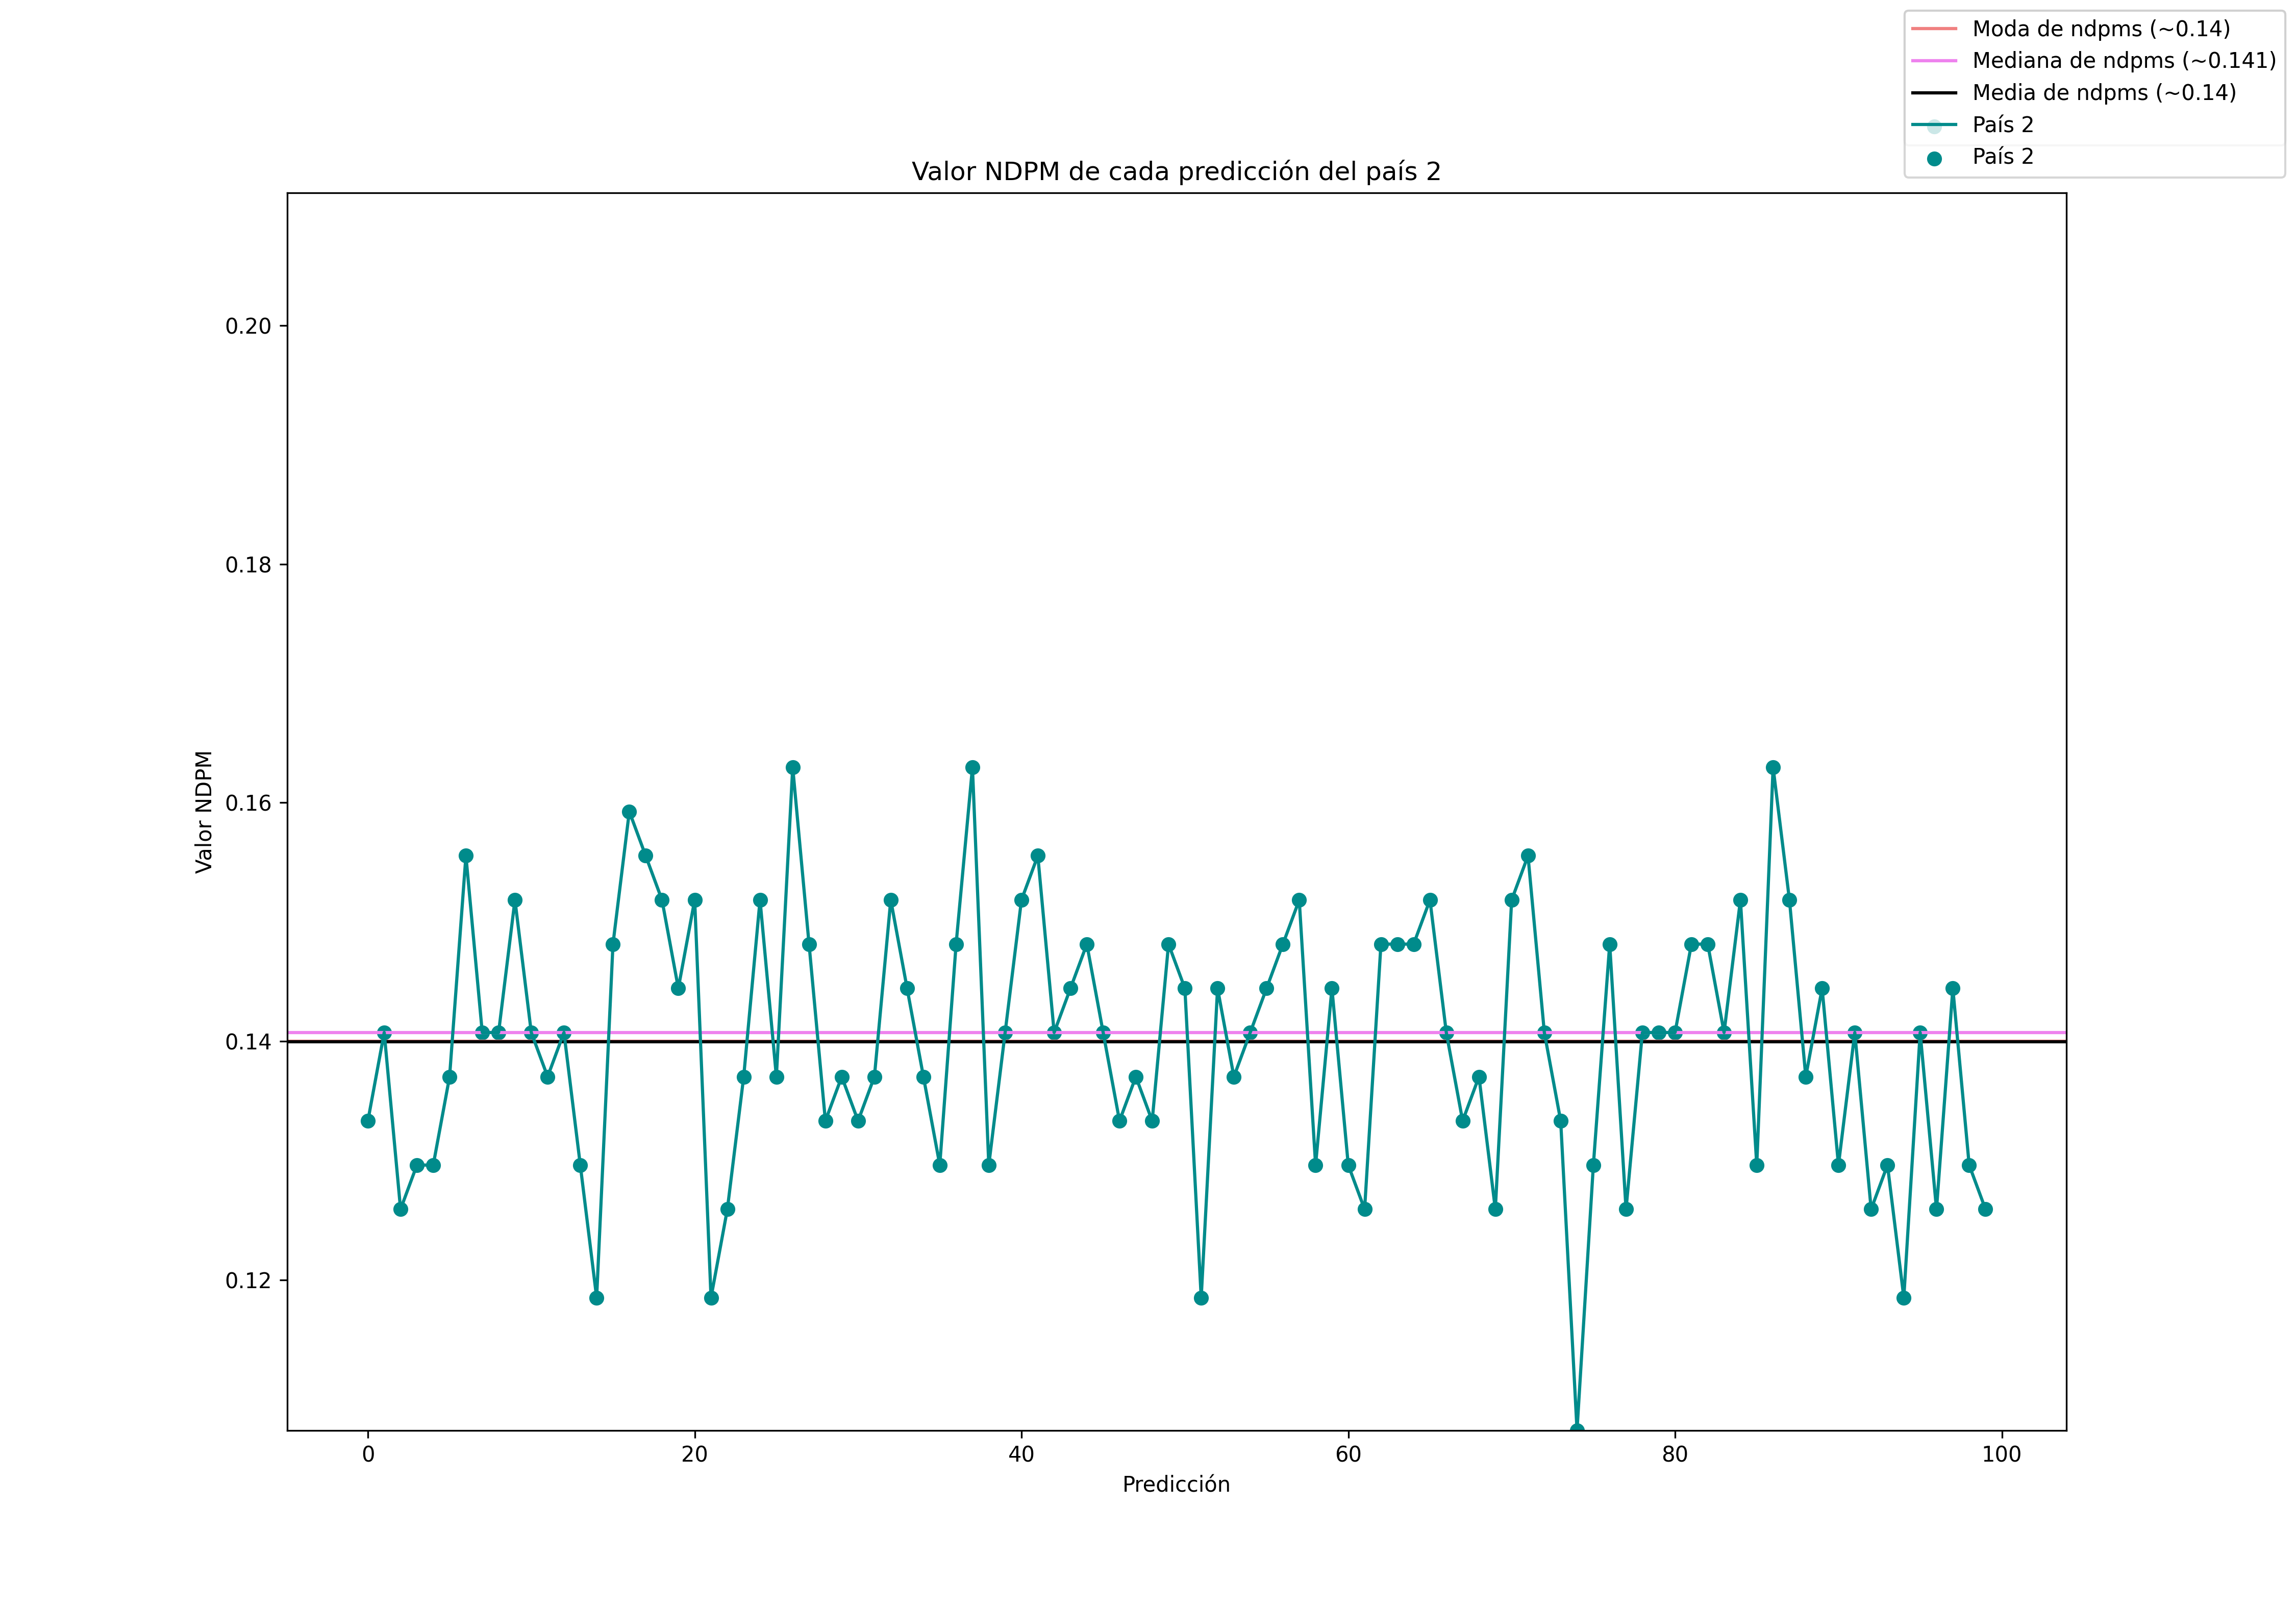
\includegraphics[width=0.5\textheight]
        {Figuras/Reports/PI_2_W1_EXT_DISP.png}}
    \caption{Gráfico de los valores NDPM del participante 2\label{fig:PI2_DISP}}
\end{sidewaysfigure}
\clearpage

\paragraph{Detalle de los resultados del participante 3}
Como se puede observar en los gráficos \ref{fig:PI3_CAJAS} y \ref{fig:PI3_DISP}, los valores del modelo original del participante 3 siempre se mantienen parecidos a los del modelo reentrenado en el servidor de FL, con \textit{W$_c$ $=1$} el valor del modelo reentrenado es peor que el original pero con \textit{W$_c$ $=0$} el valor del modelo reentrenado es mejor que el original. En los gráficos se pueden observar varias líneas horizontales que hacen referencia a la media, mediana y moda, dibujadas en negro, rosa y marrón respectivamente.

\paragraph{Detalle de los resultados del participante 4}
Como se puede observar en los gráficos \ref{fig:PI4_CAJAS} y \ref{fig:PI4_DISP}, los valores del modelo original del participante 4 siempre se mantienen por debajo de los del modelo reentrenado en el servidor de FL, tanto con \textit{W$_c$ $=1$} como con \textit{W$_c$ $=0$}, aunque no con tanta diferencia como el participante 2. En los gráficos se pueden observar varias líneas horizontales que hacen referencia a la media, mediana y moda, dibujadas en negro, rosa y marrón respectivamente.

\begin{sidewaysfigure}
    \centering
    \subfloat[Modelo original]
        {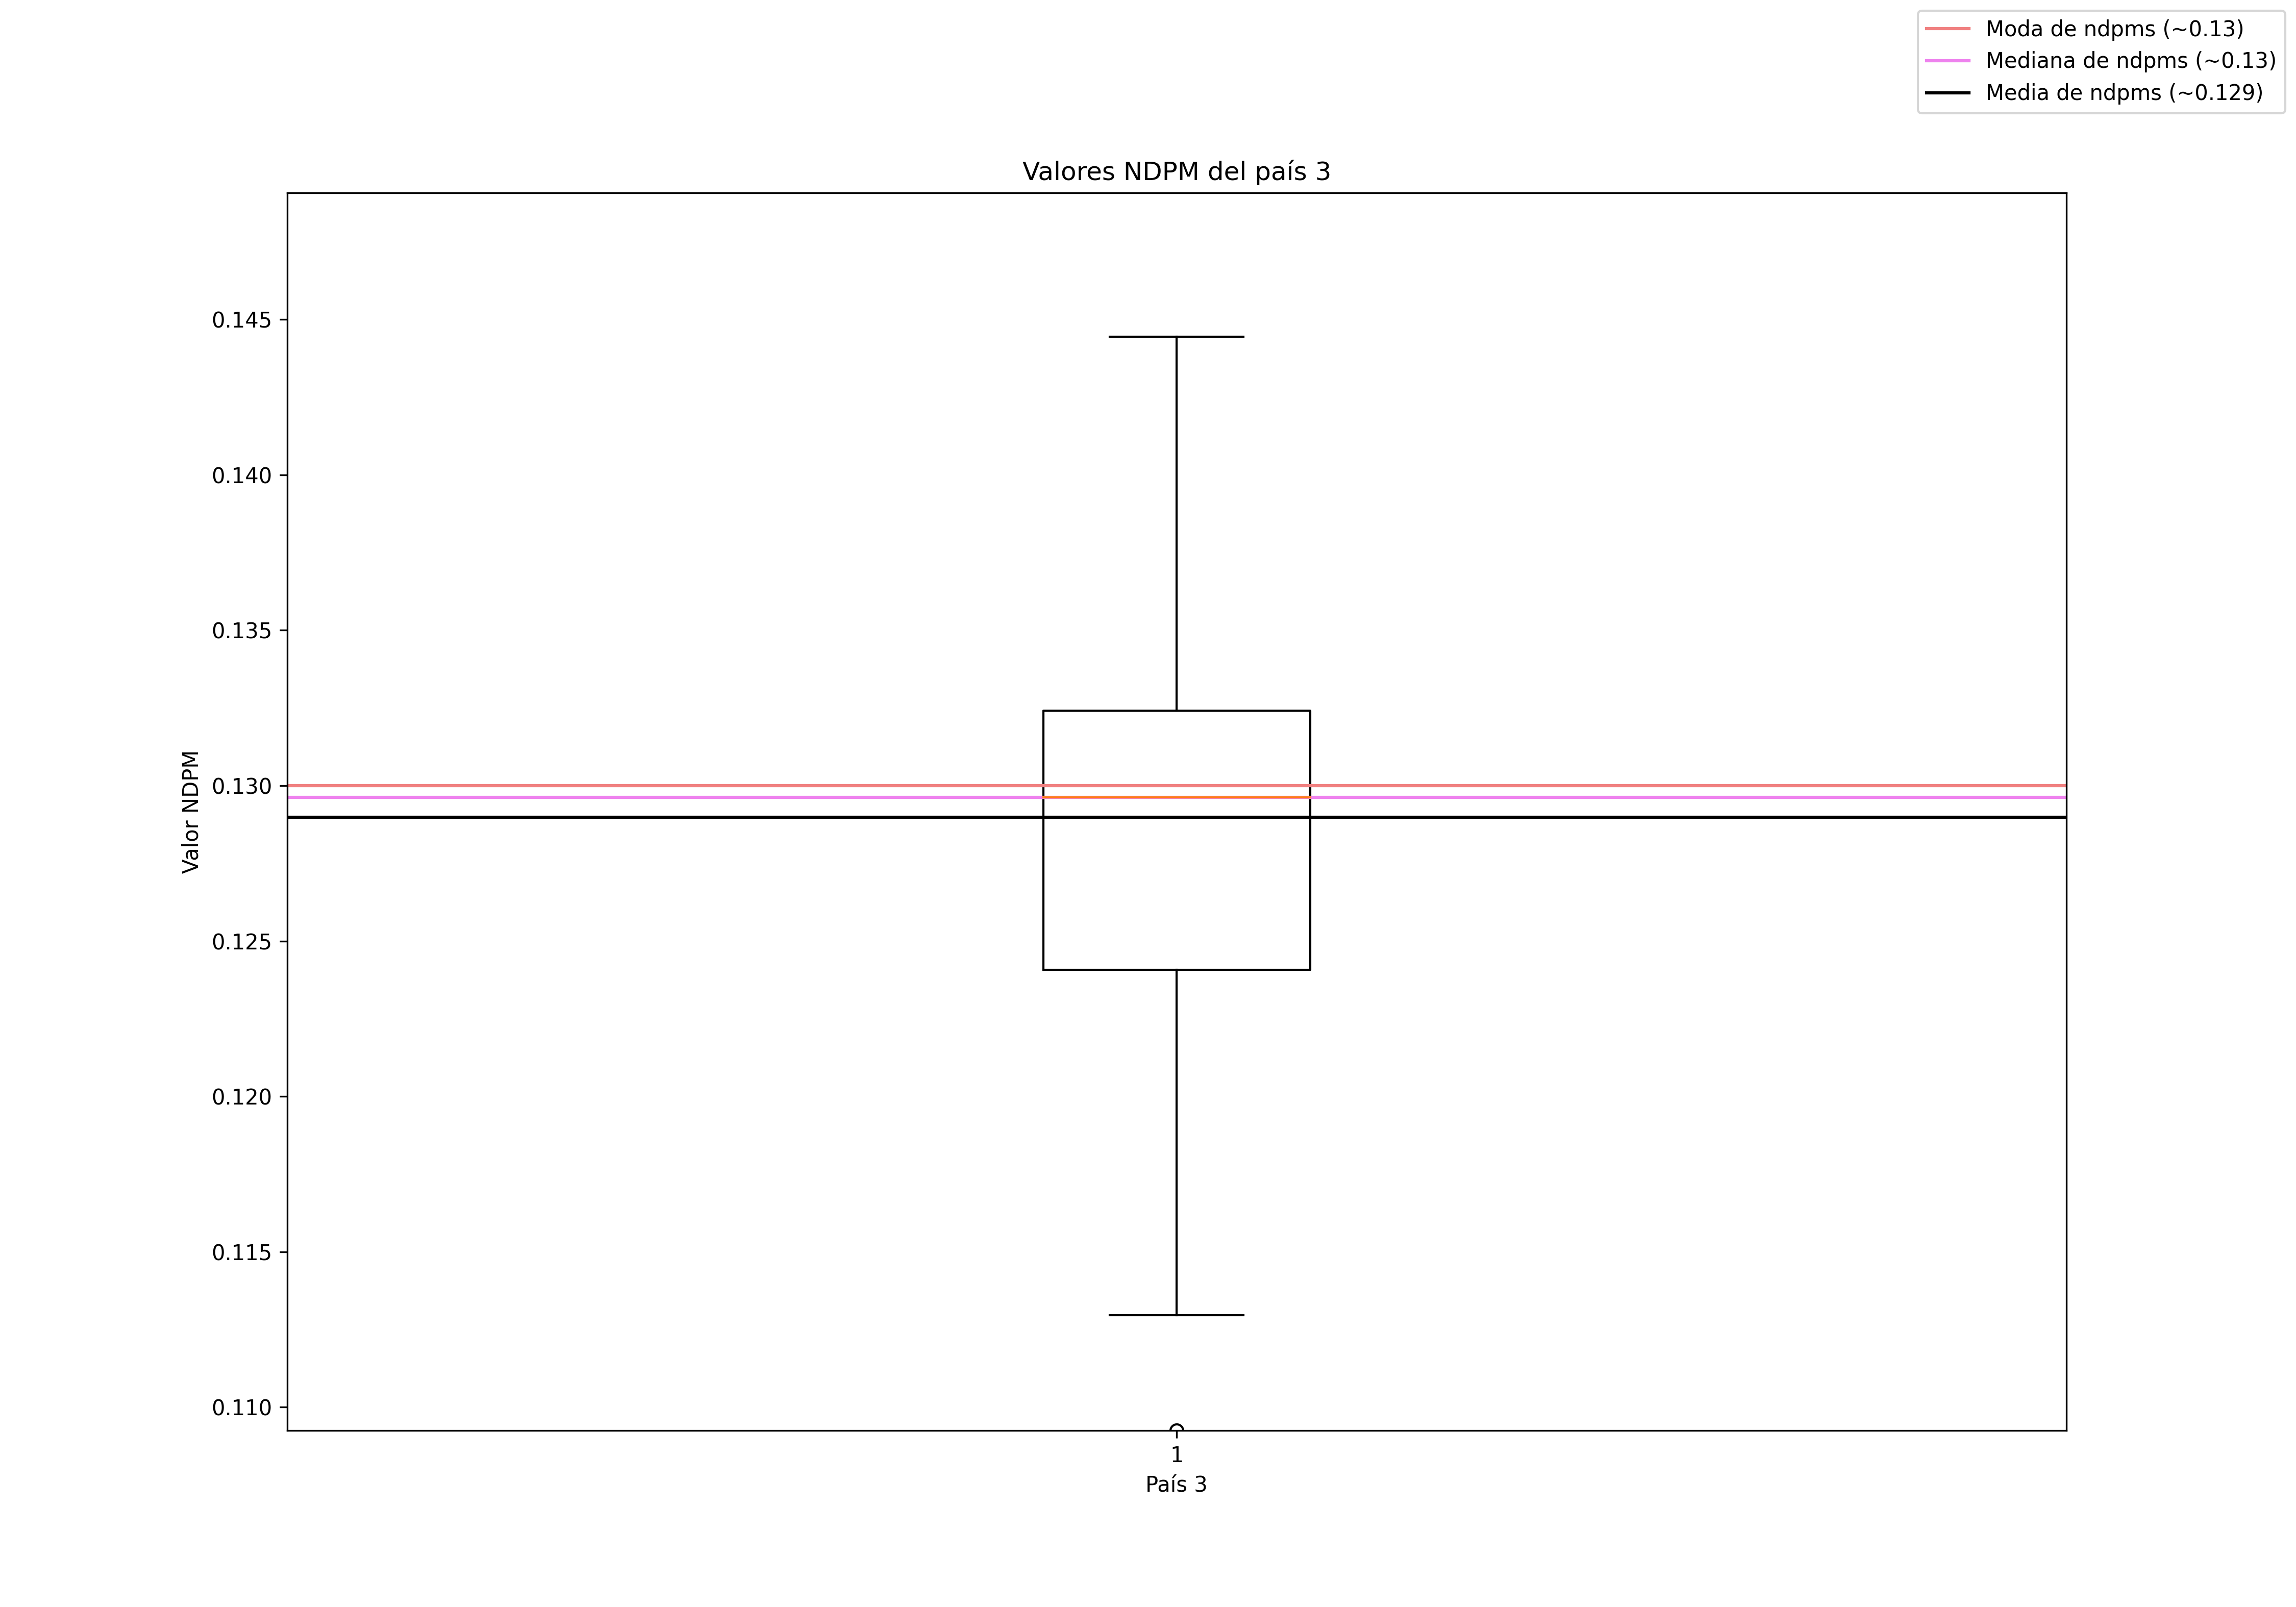
\includegraphics[width=0.5\textheight]
        {Figuras/Reports/PI_3_W0_LOC_CAJAS.png}}
        \quad
    \subfloat[Reentrenado con \textit{W$_c$ $=0$}]
        {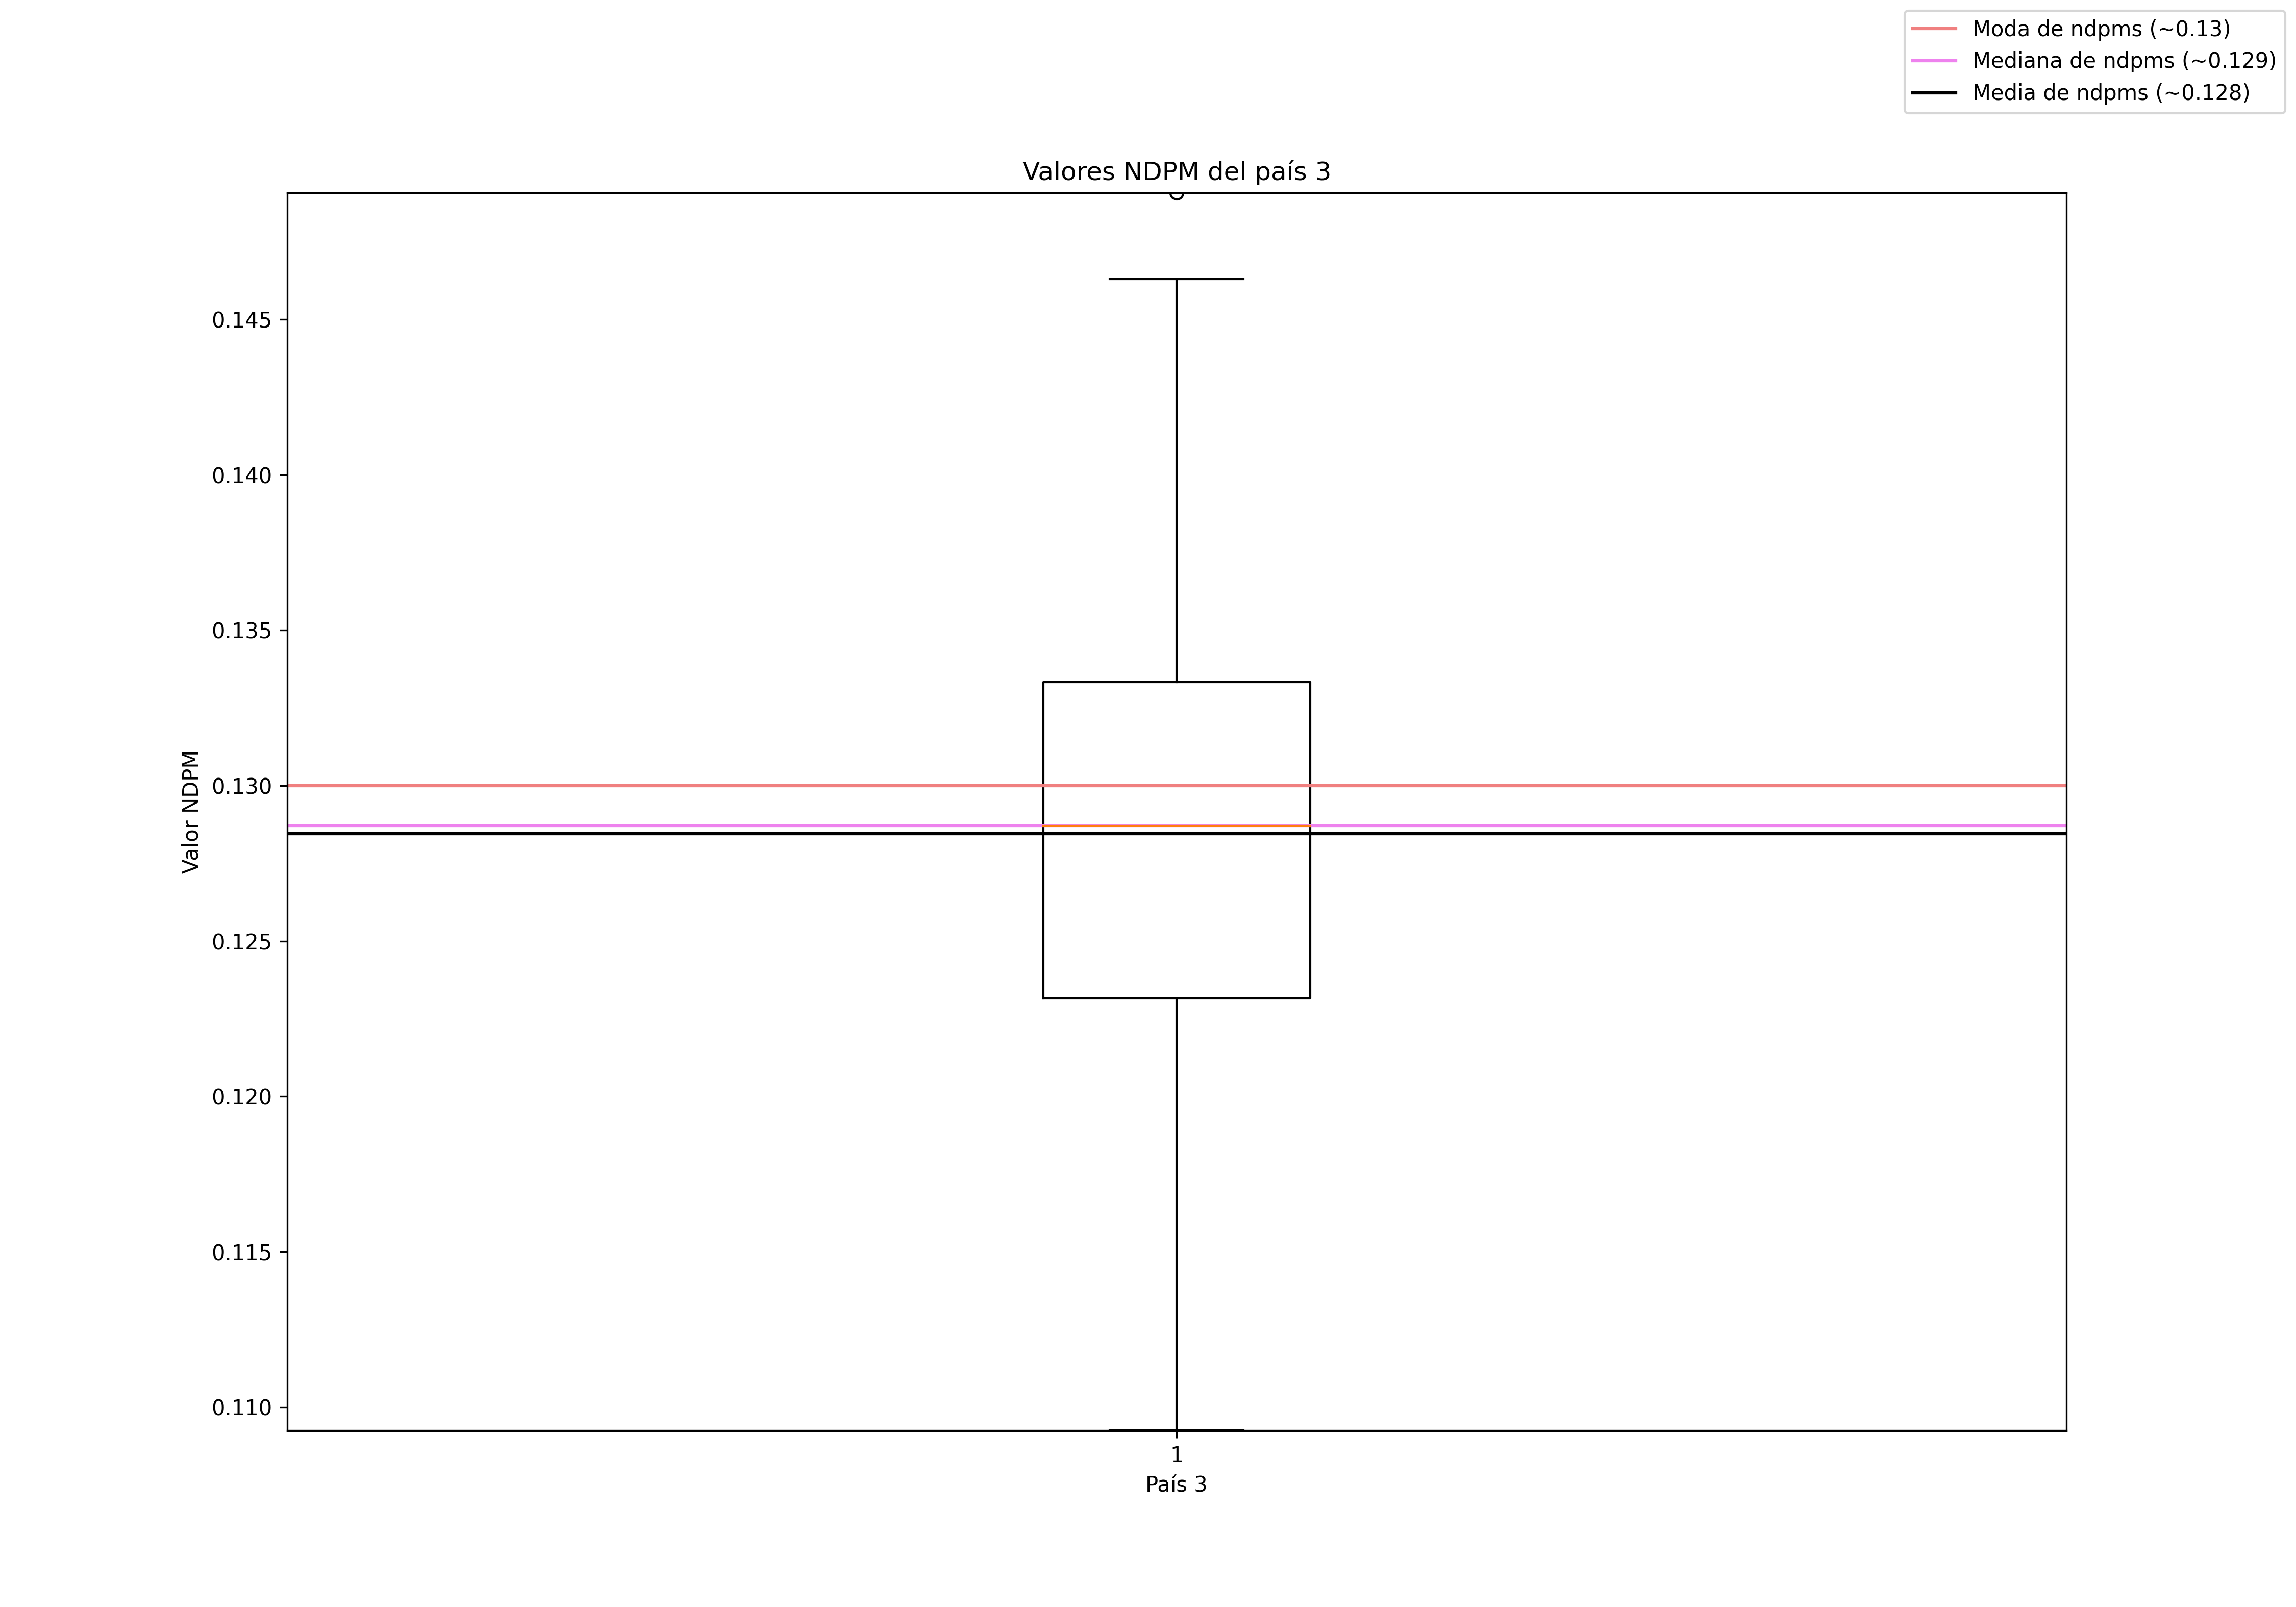
\includegraphics[width=0.5\textheight]
        {Figuras/Reports/PI_3_W0_EXT_CAJAS.png}}
    \subfloat[Reentrenado con \textit{W$_c$ $=1$}]{
        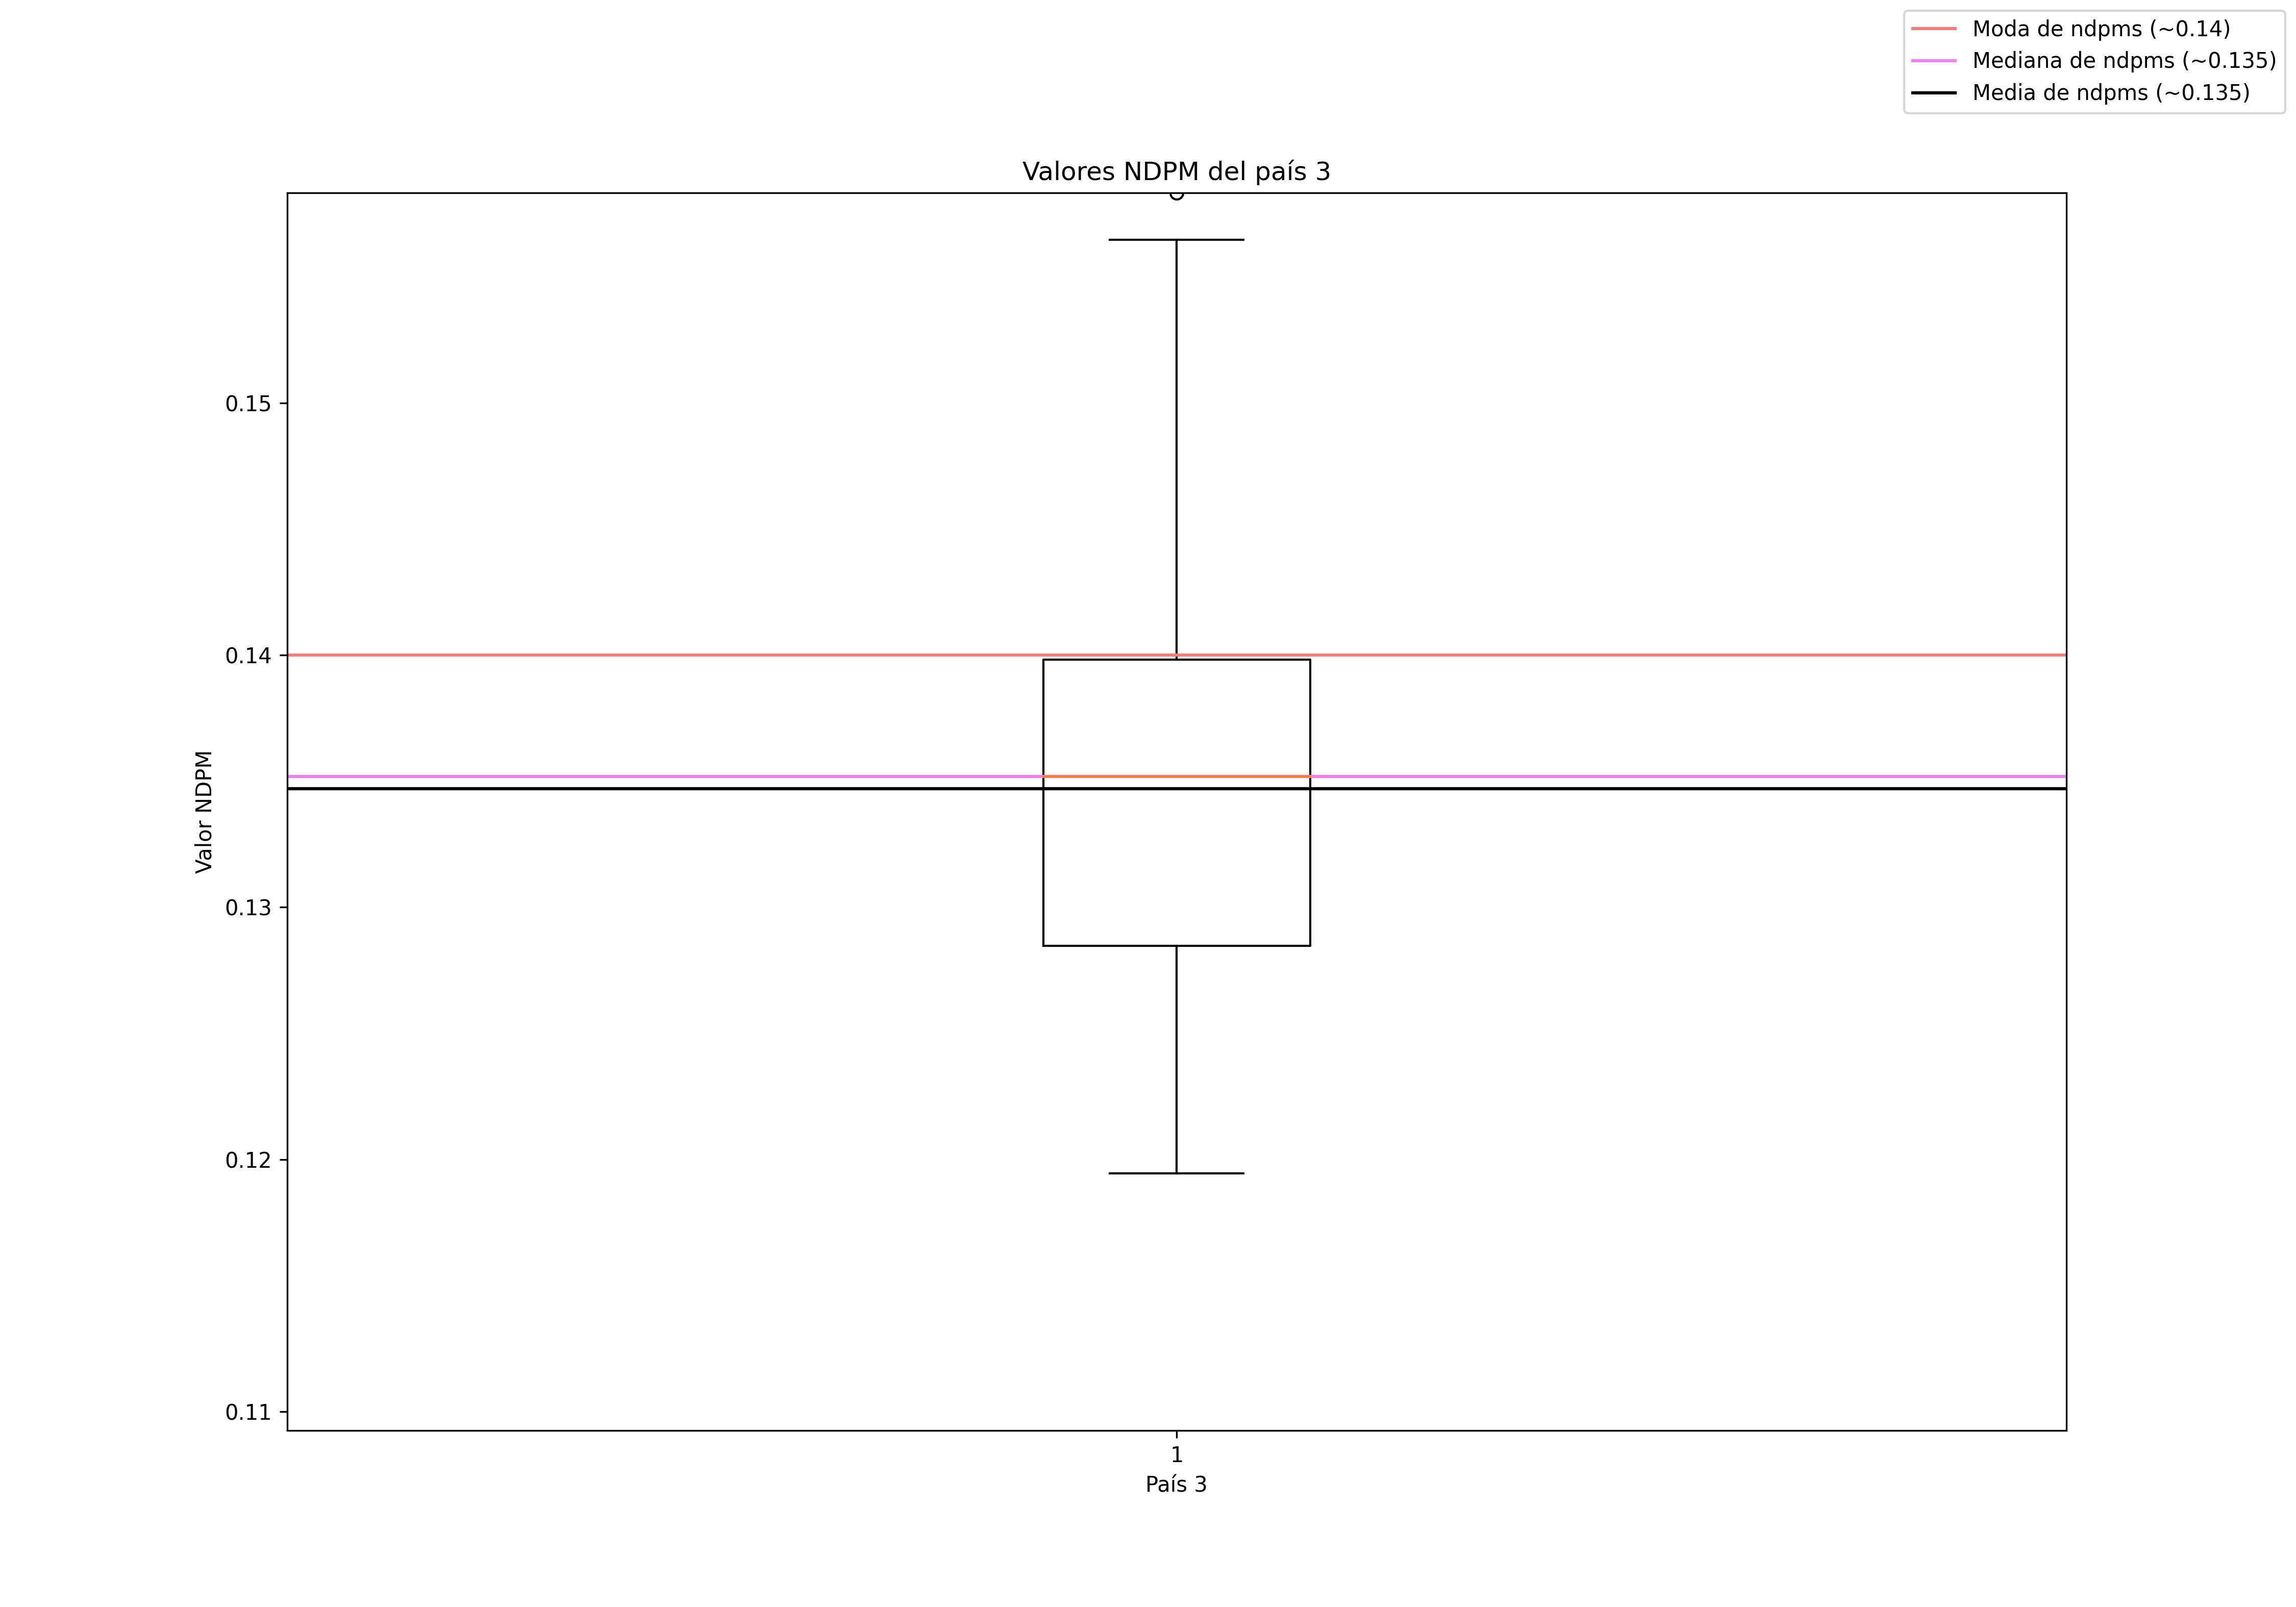
\includegraphics[width=0.5\textheight]
        {Figuras/Reports/PI_3_W1_EXT_CAJAS.png}}
    \caption{Diagramas de cajas y bigotes de los valores NDPM del participante 3\label{fig:PI3_CAJAS}}
\end{sidewaysfigure}
\clearpage
\begin{sidewaysfigure}
    \centering
    \subfloat[Modelo original]
        {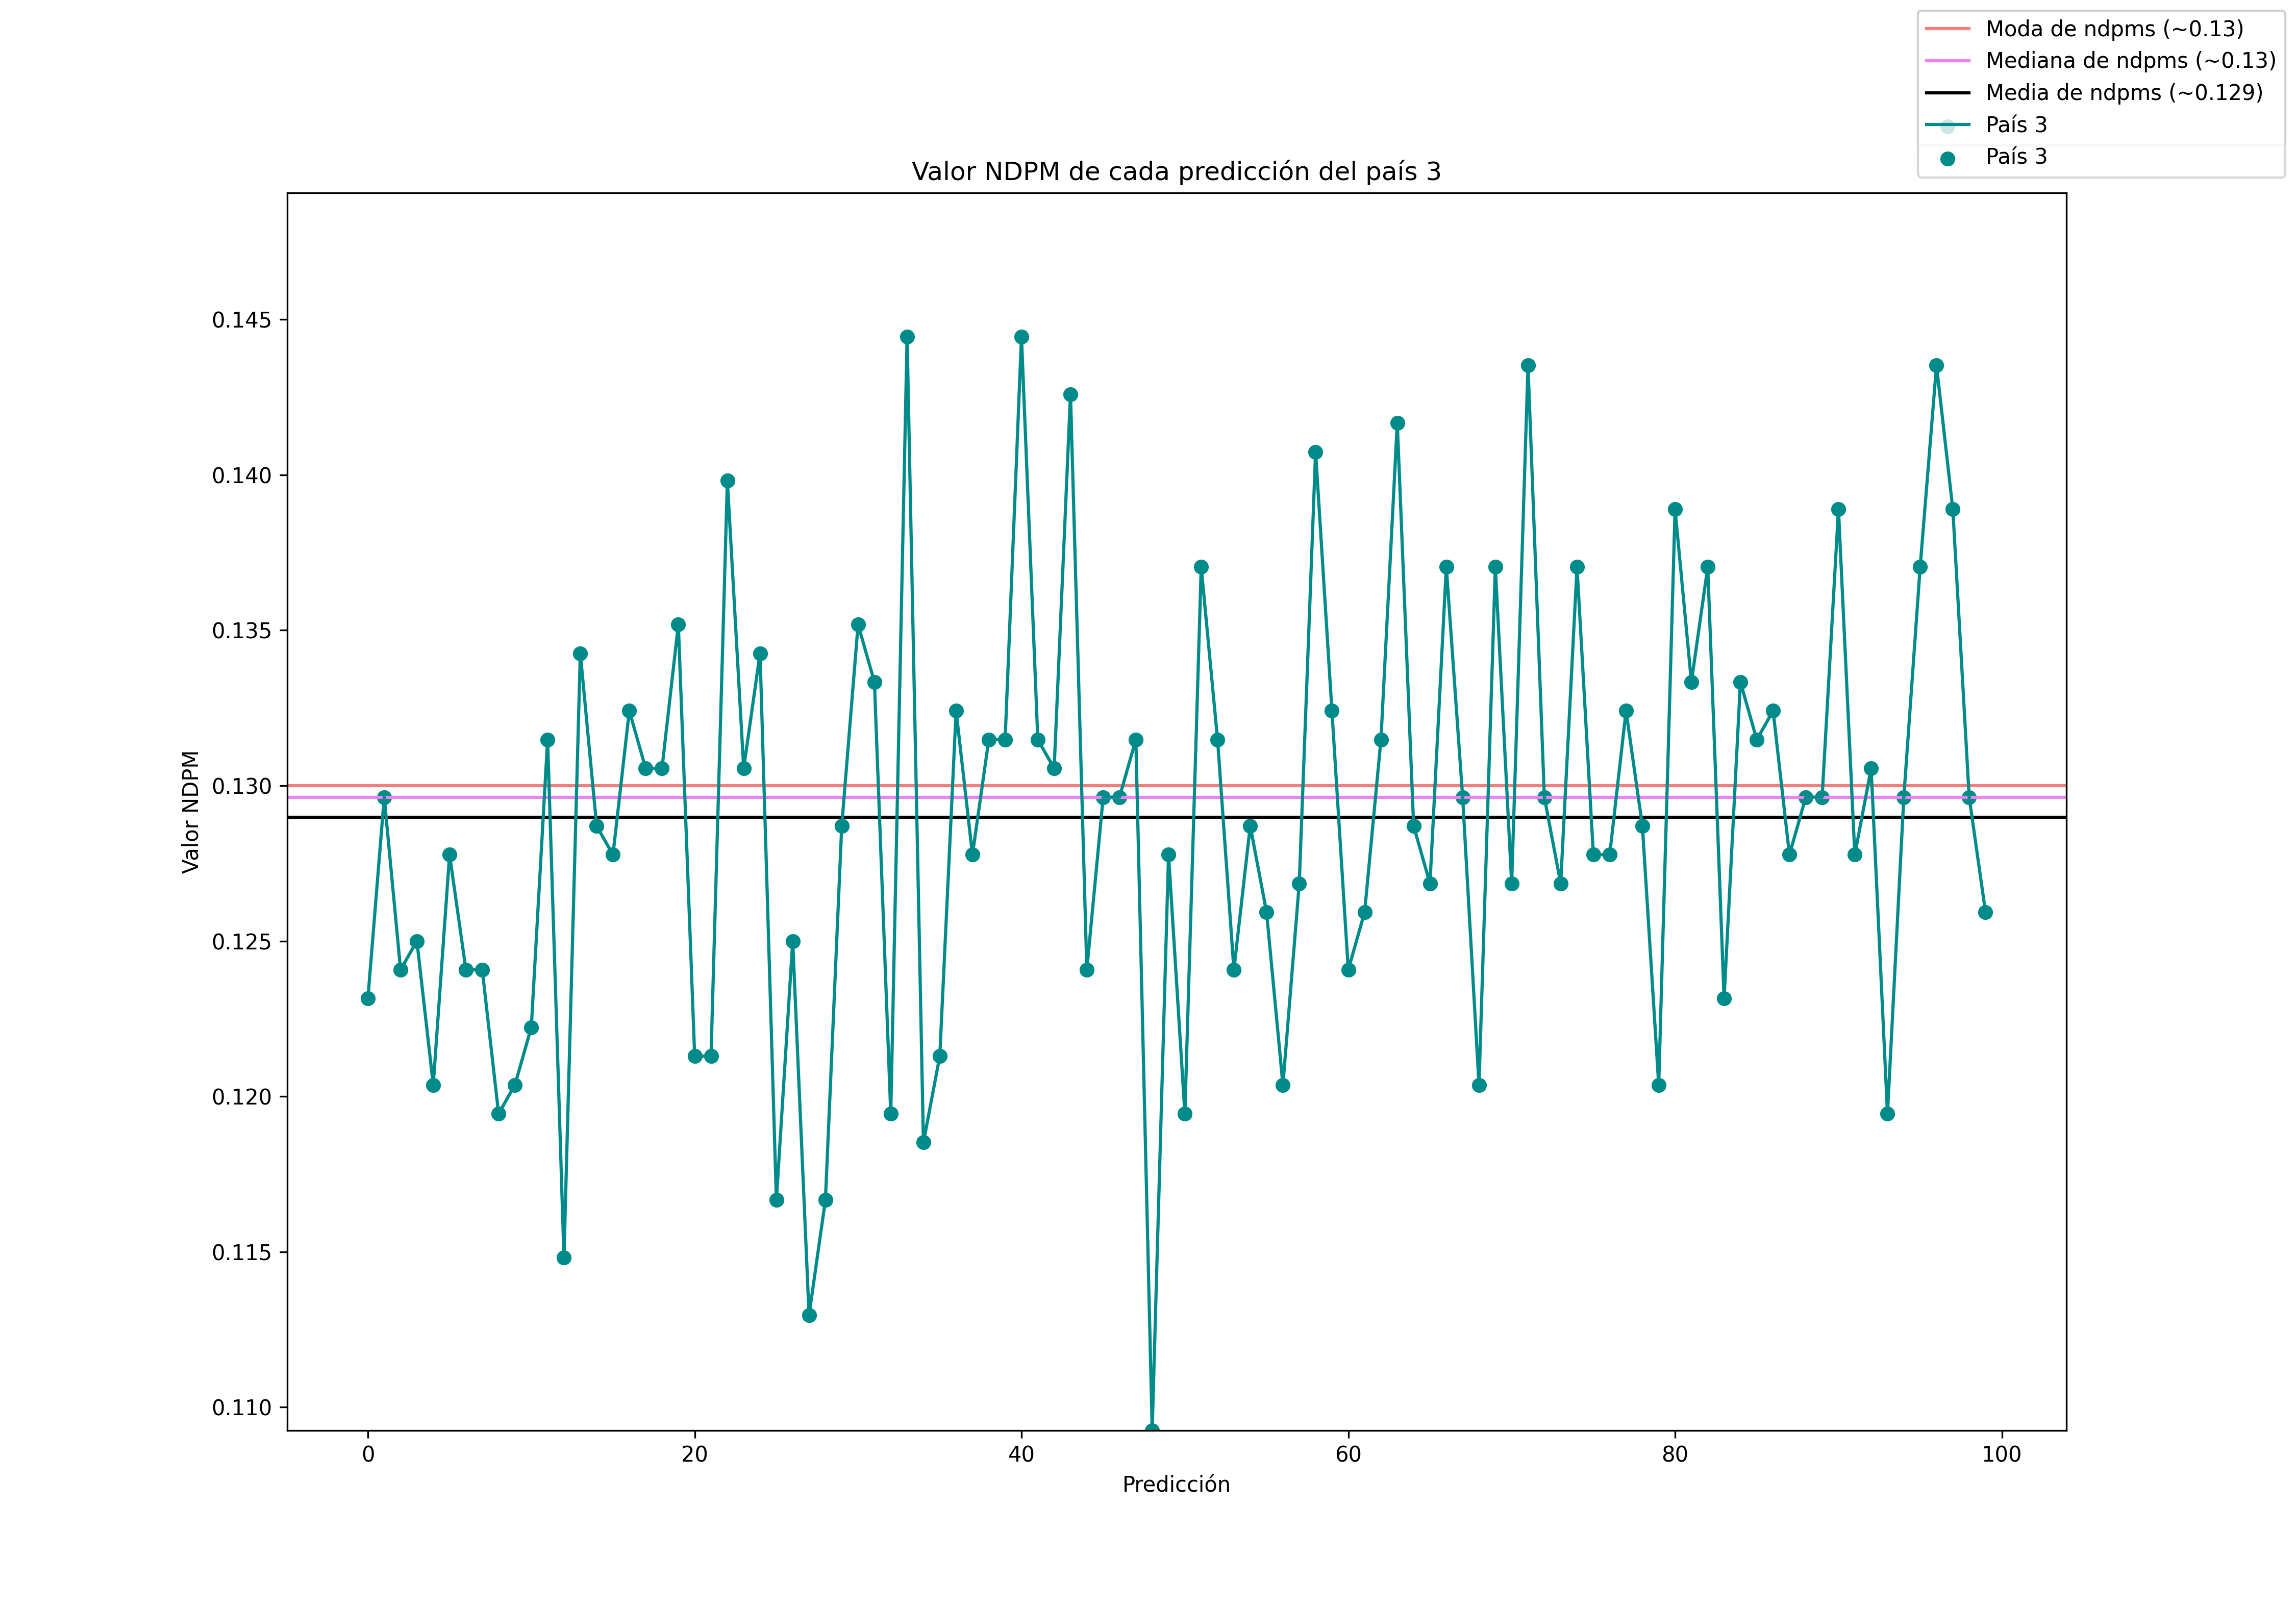
\includegraphics[width=0.5\textheight]
        {Figuras/Reports/PI_3_W0_LOC_DISP.png}}
        \quad
    \subfloat[Reentrenado con \textit{W$_c$ $=0$}]
        {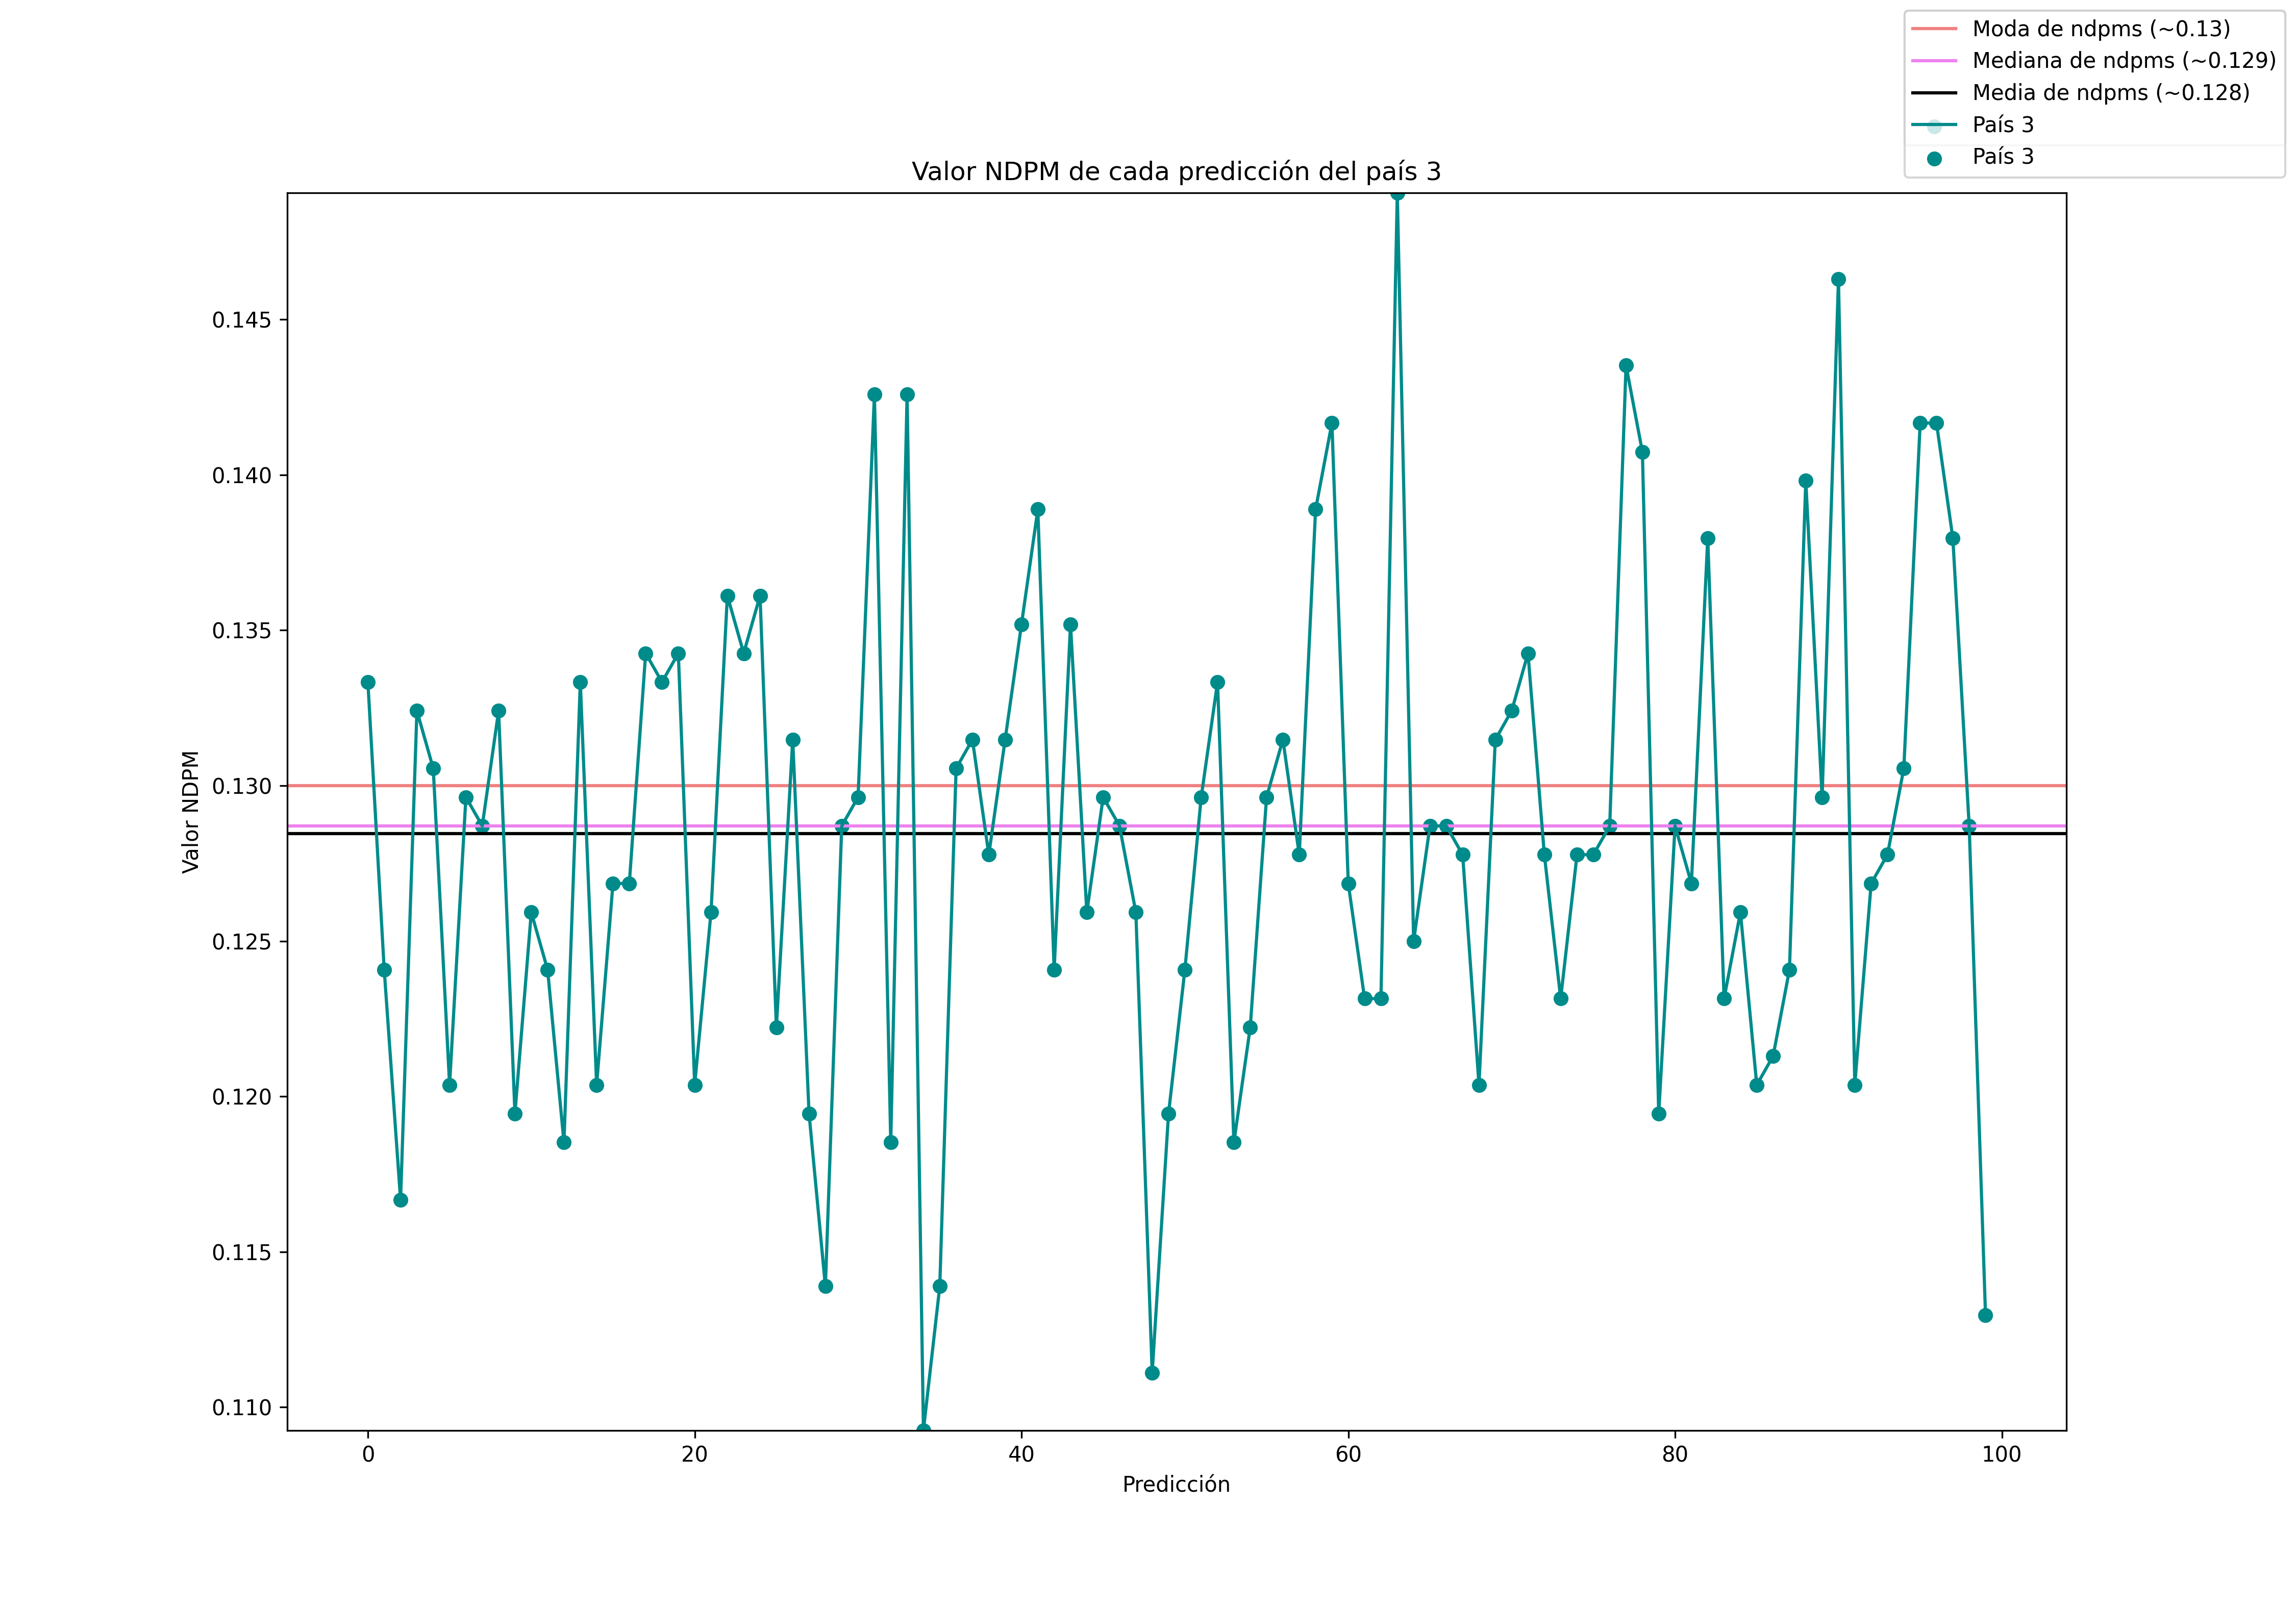
\includegraphics[width=0.5\textheight]
        {Figuras/Reports/PI_3_W0_EXT_DISP.png}}
    \subfloat[Reentrenado con \textit{W$_c$ $=1$}]{
        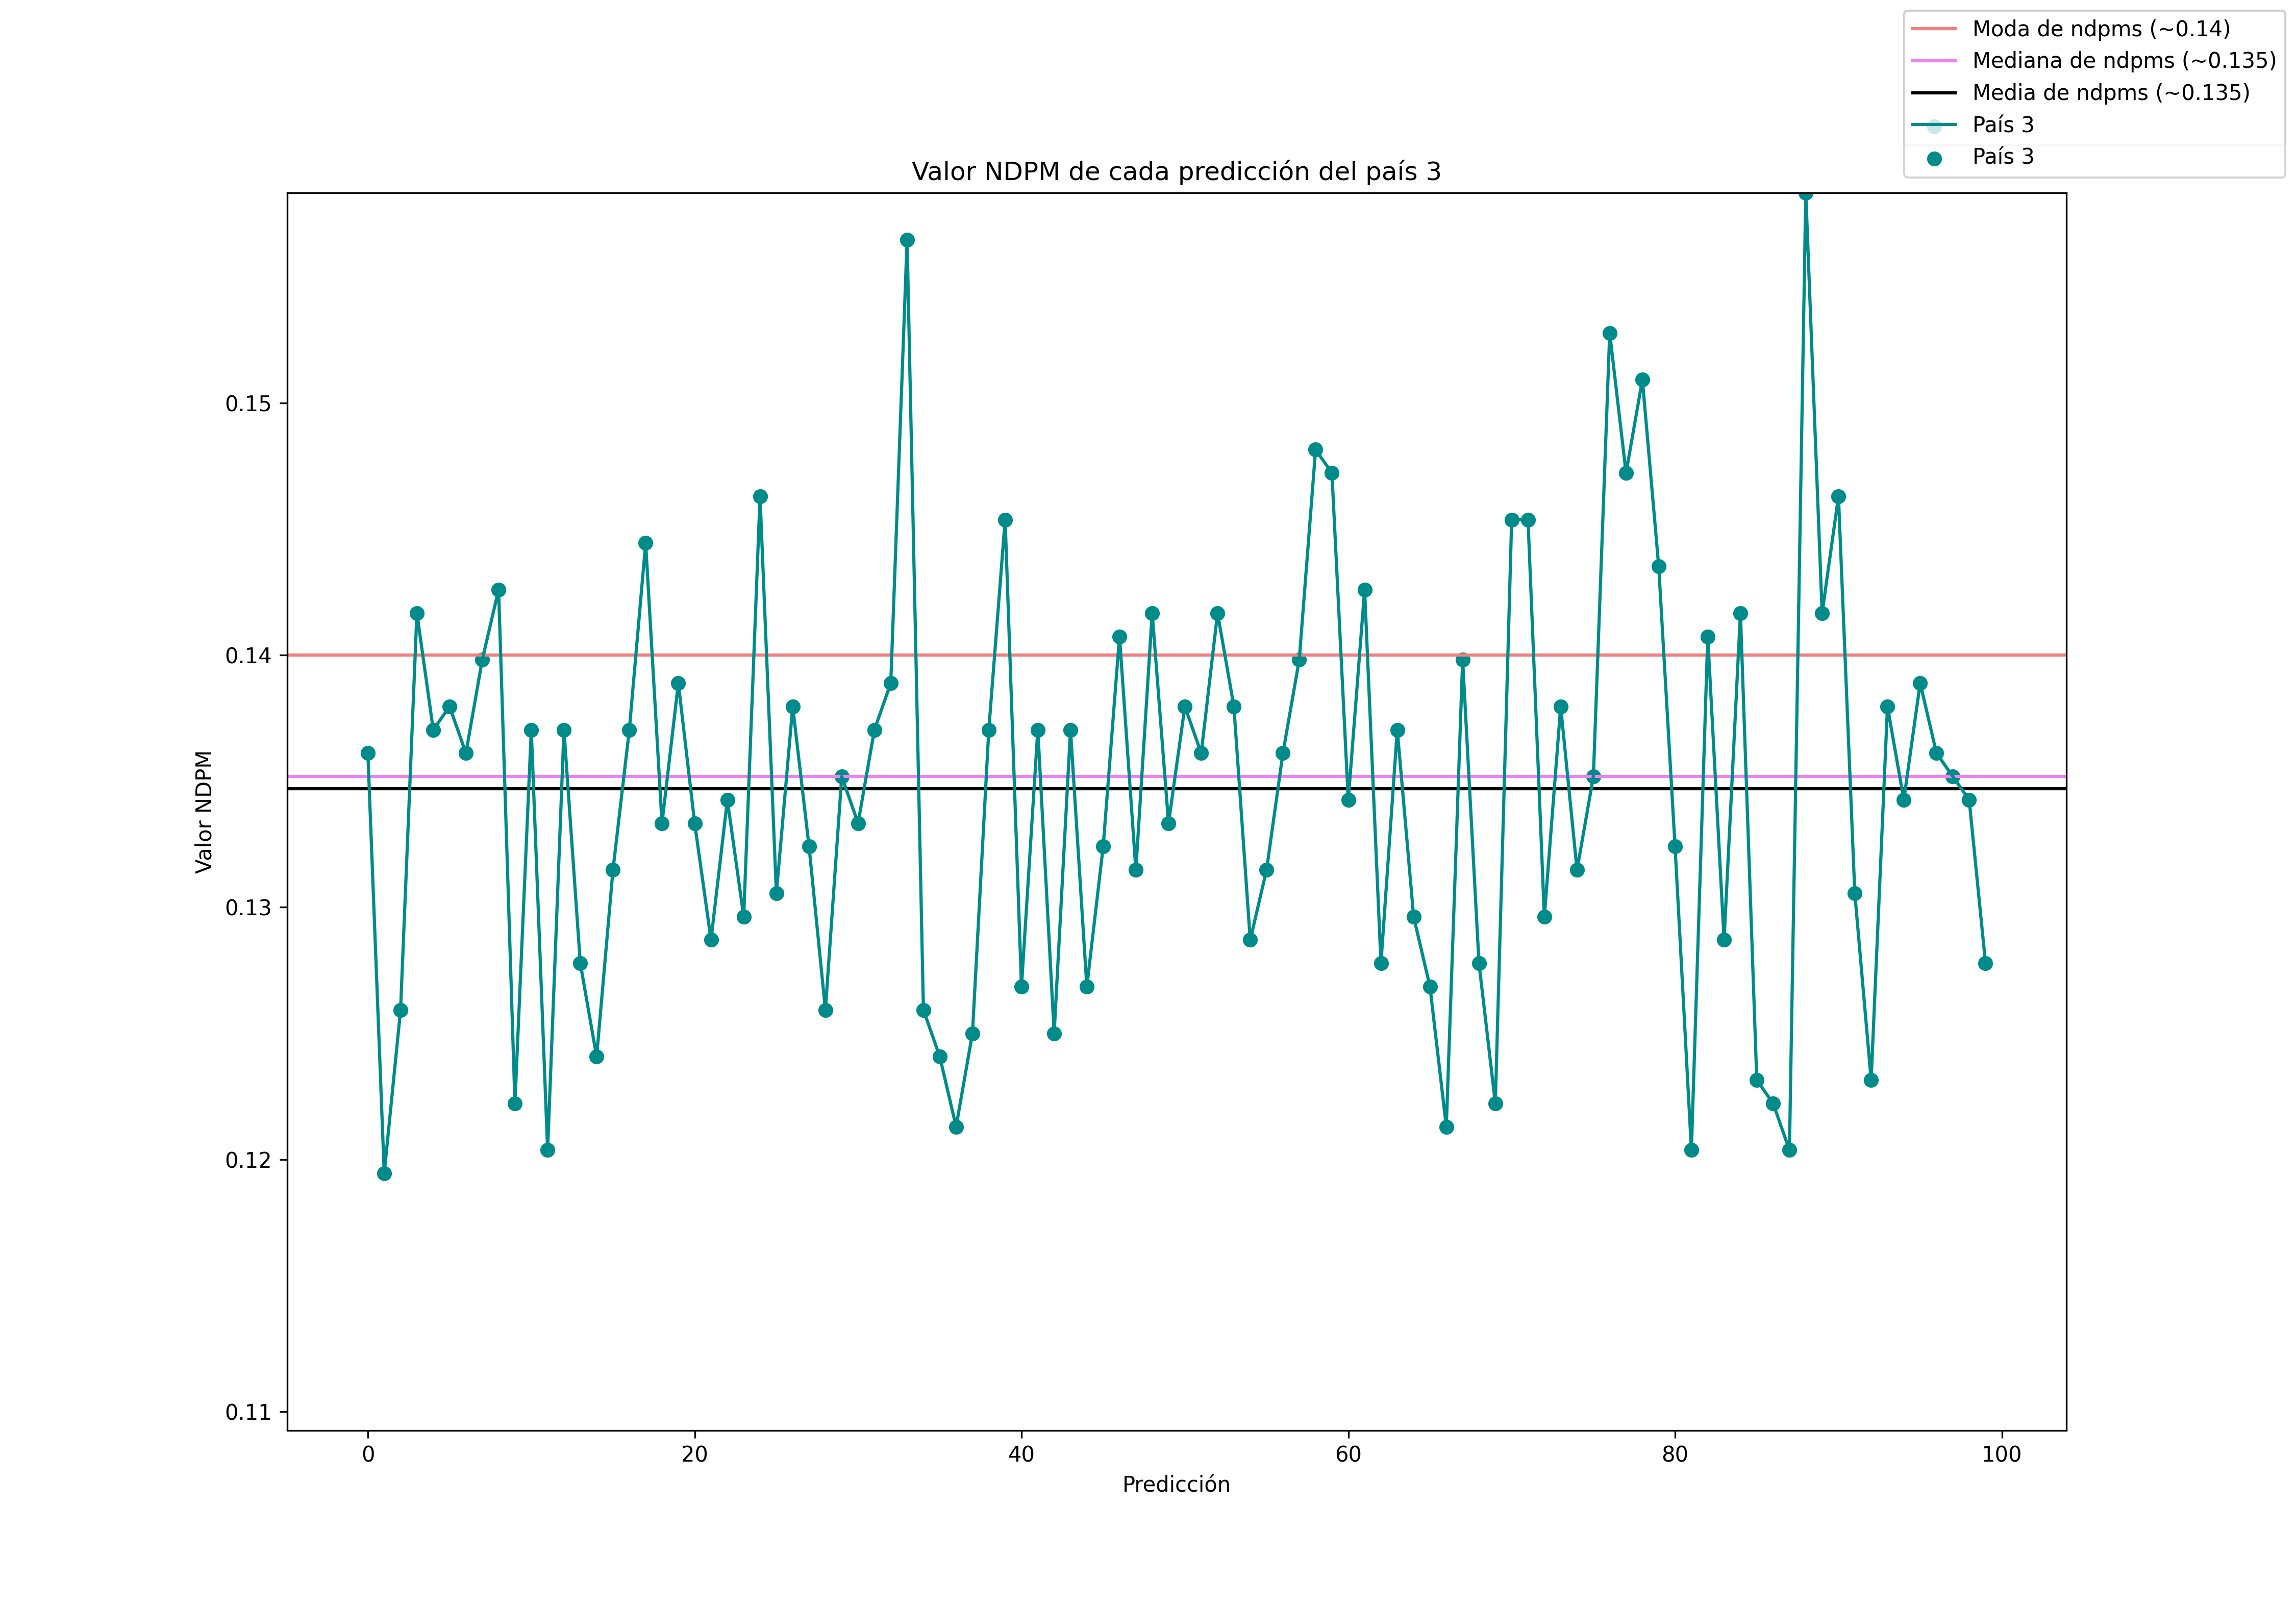
\includegraphics[width=0.5\textheight]
        {Figuras/Reports/PI_3_W1_EXT_DISP.png}}
    \caption{Gráfico de los valores NDPM del participante 3\label{fig:PI3_DISP}}
\end{sidewaysfigure}
\clearpage

\begin{sidewaysfigure}
    \centering
    \subfloat[Modelo original]
        {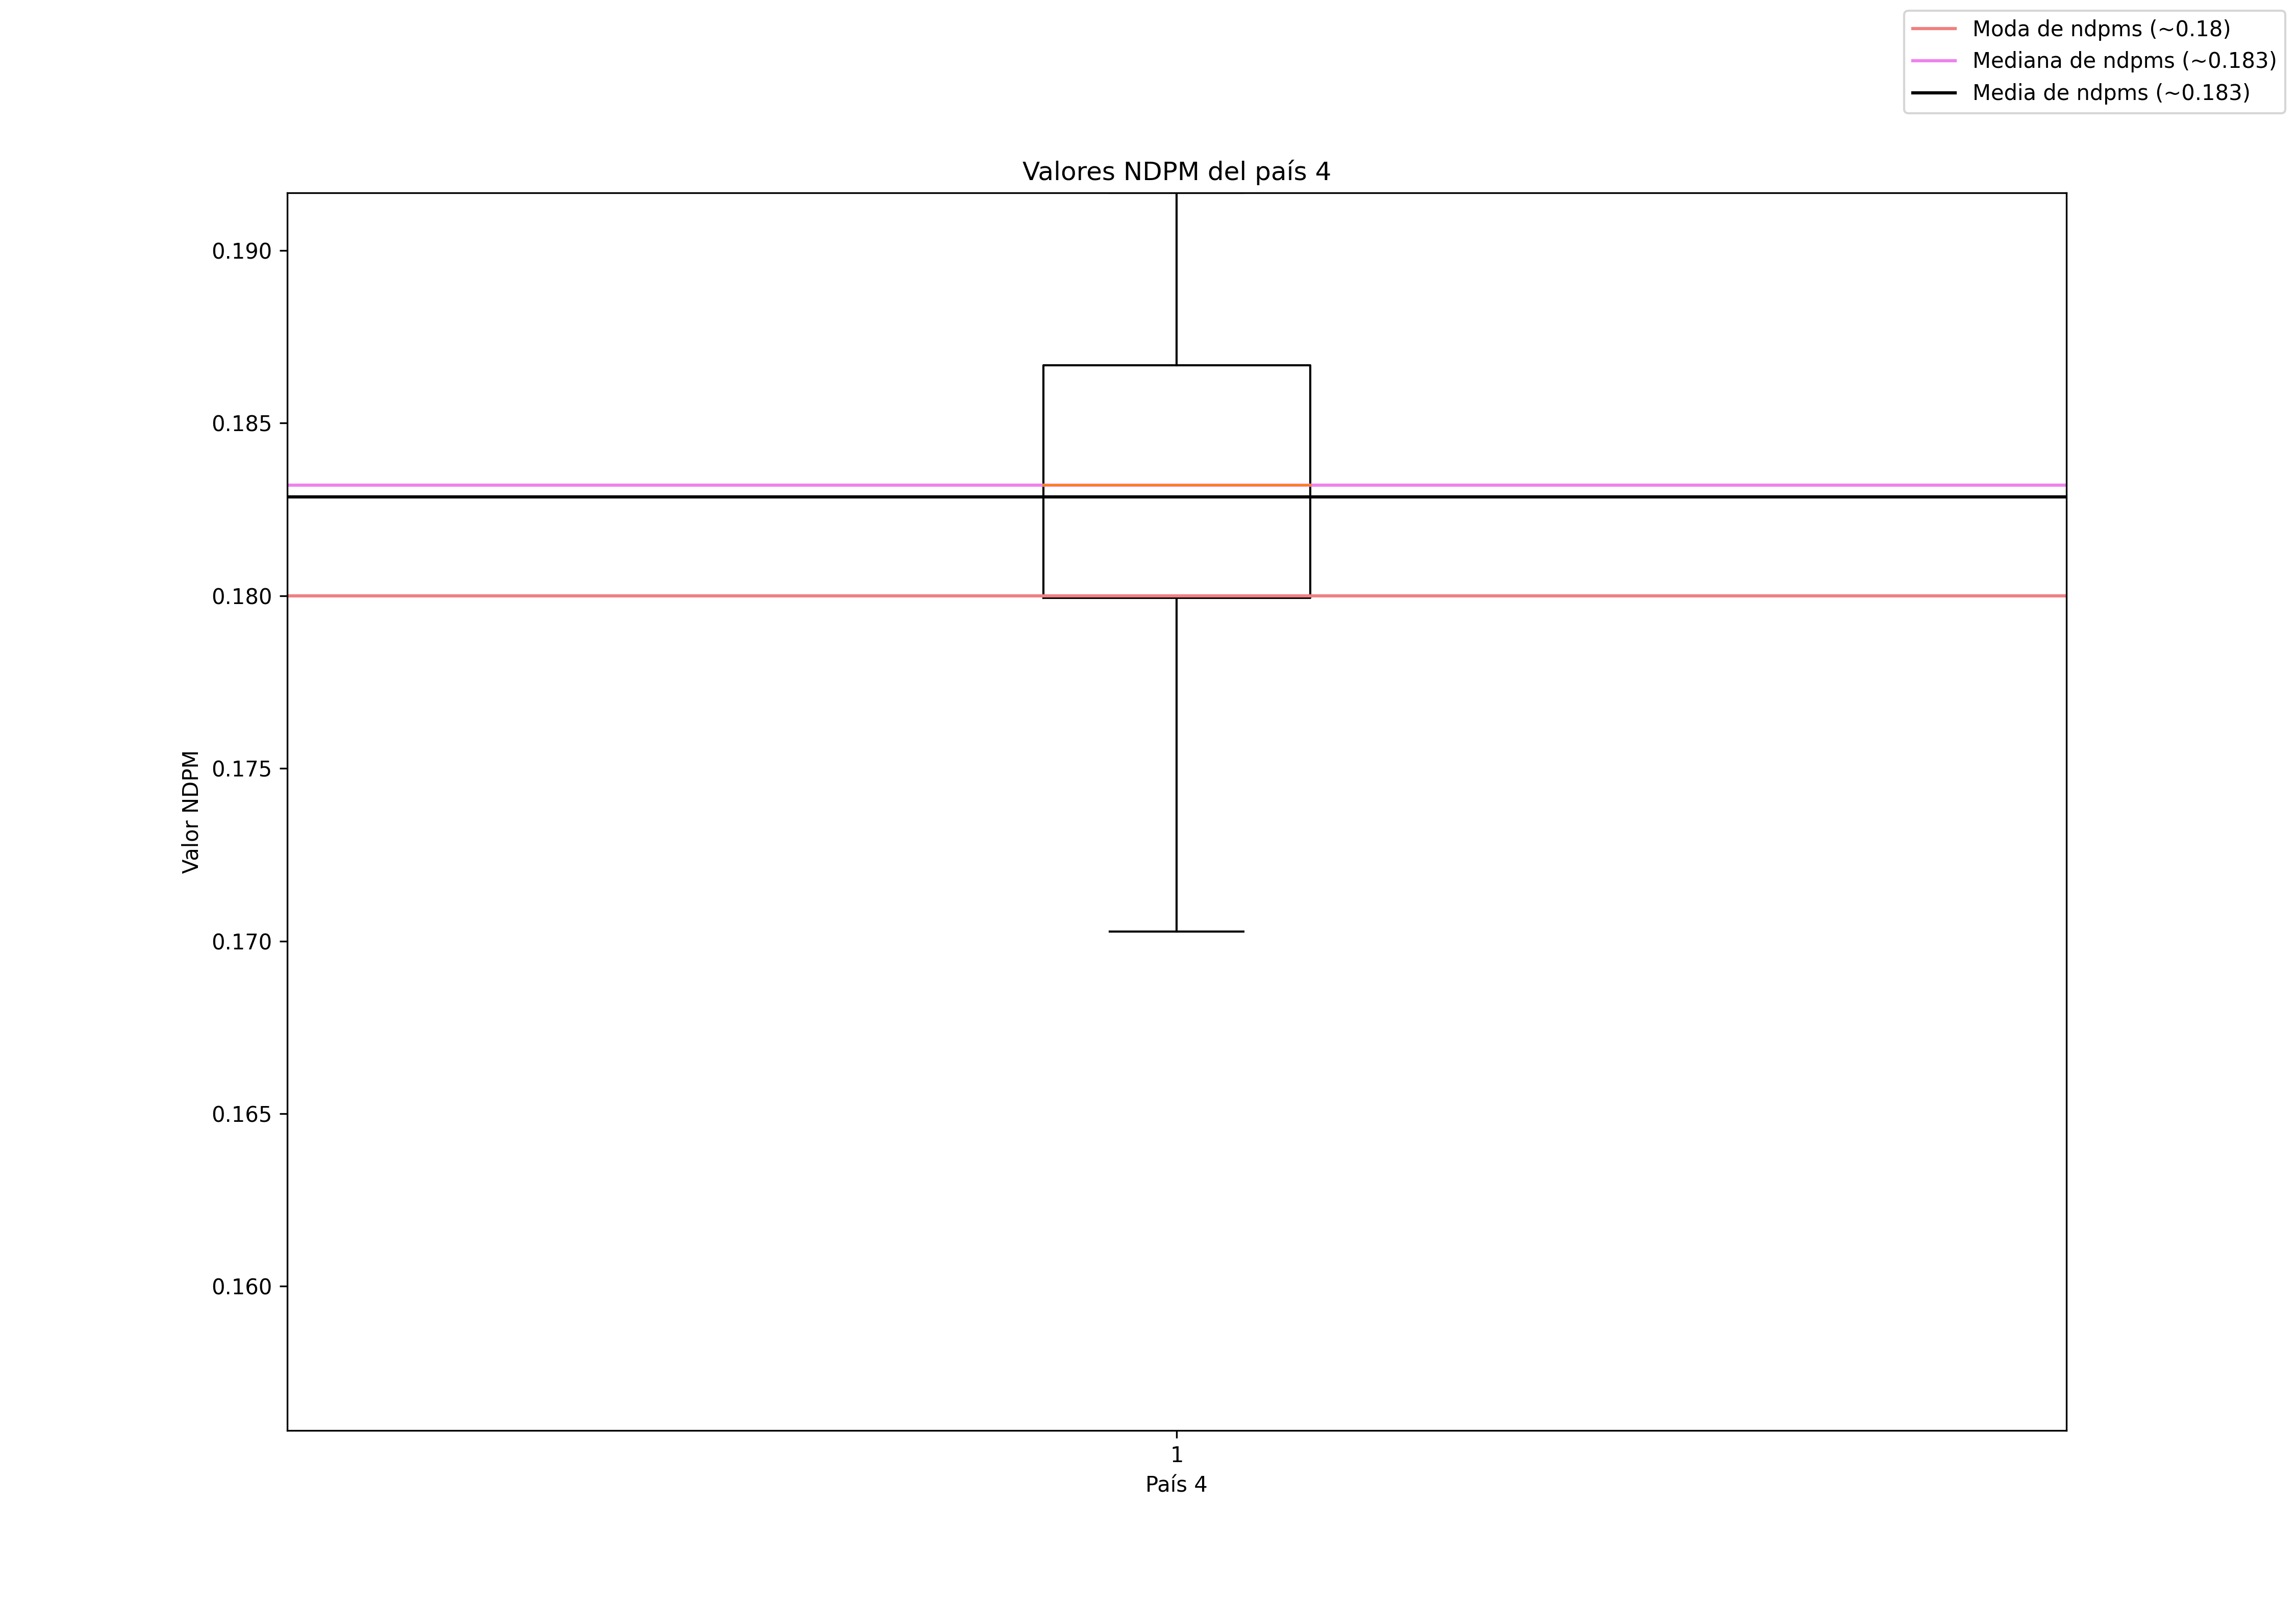
\includegraphics[width=0.5\textheight]
        {Figuras/Reports/PI_4_W0_LOC_CAJAS.png}}
        \quad
    \subfloat[Reentrenado con \textit{W$_c$ $=0$}]
        {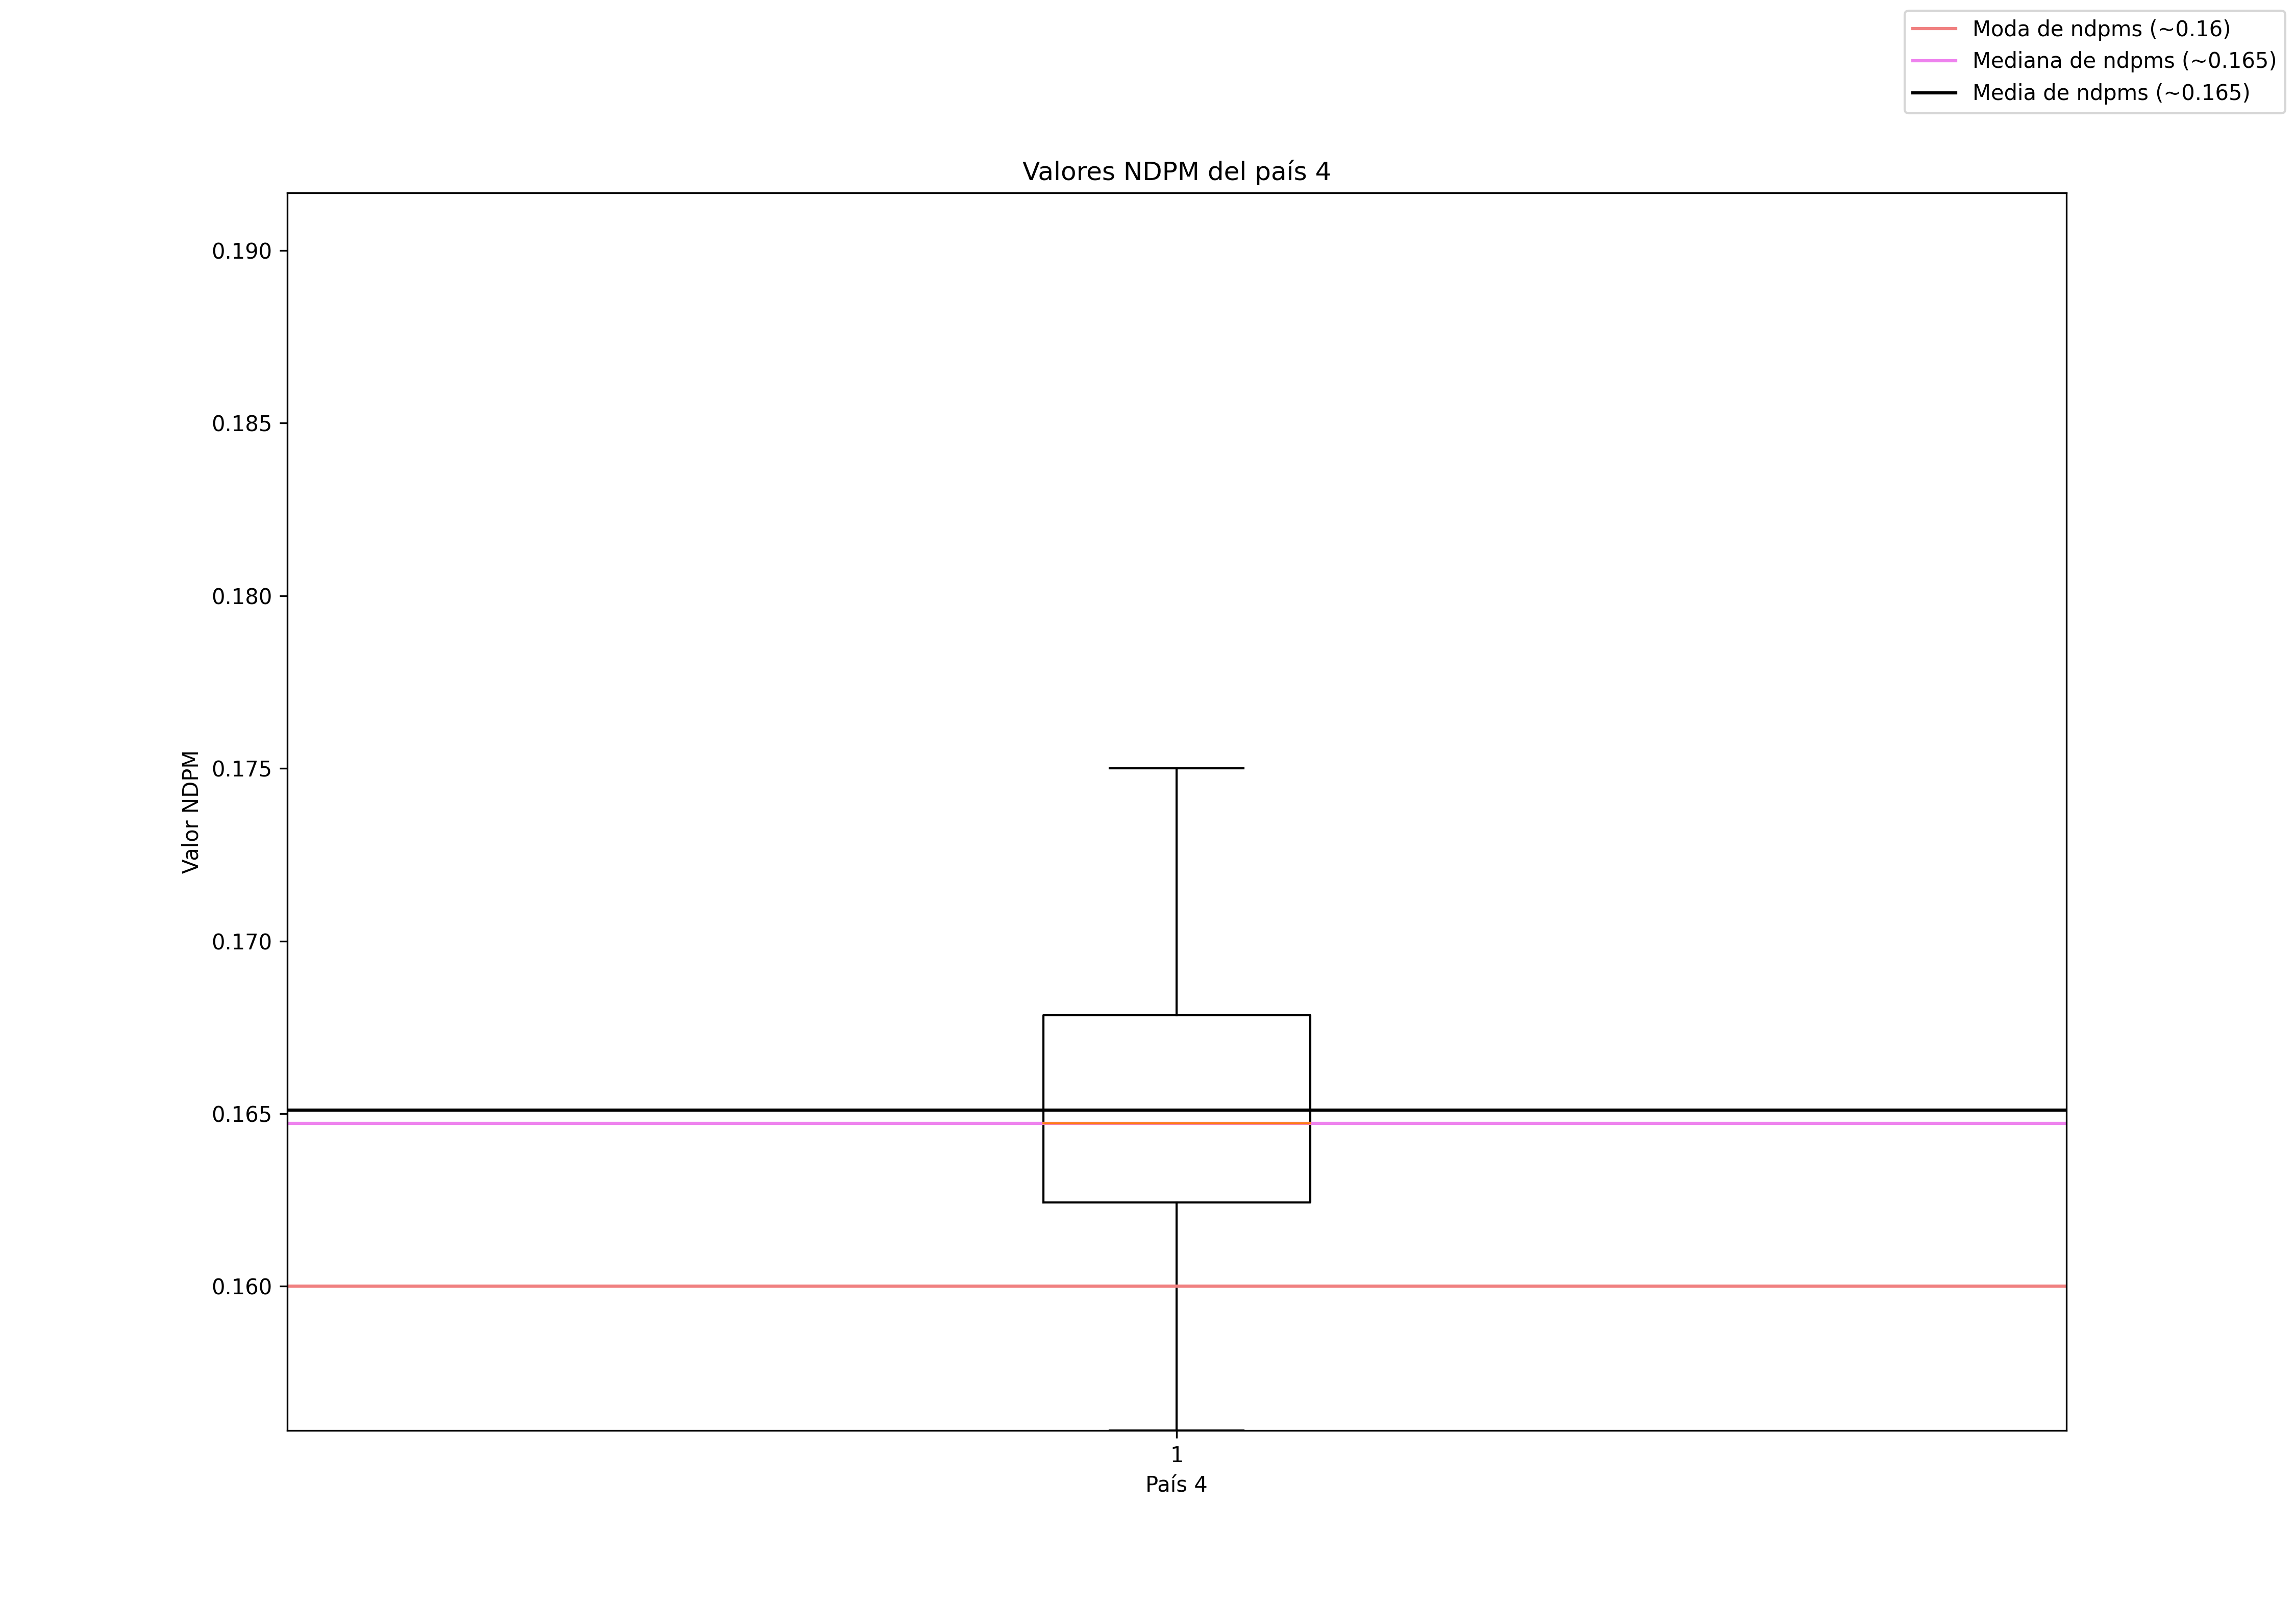
\includegraphics[width=0.5\textheight]
        {Figuras/Reports/PI_4_W0_EXT_CAJAS.png}}
    \subfloat[Reentrenado con \textit{W$_c$ $=1$}]{
        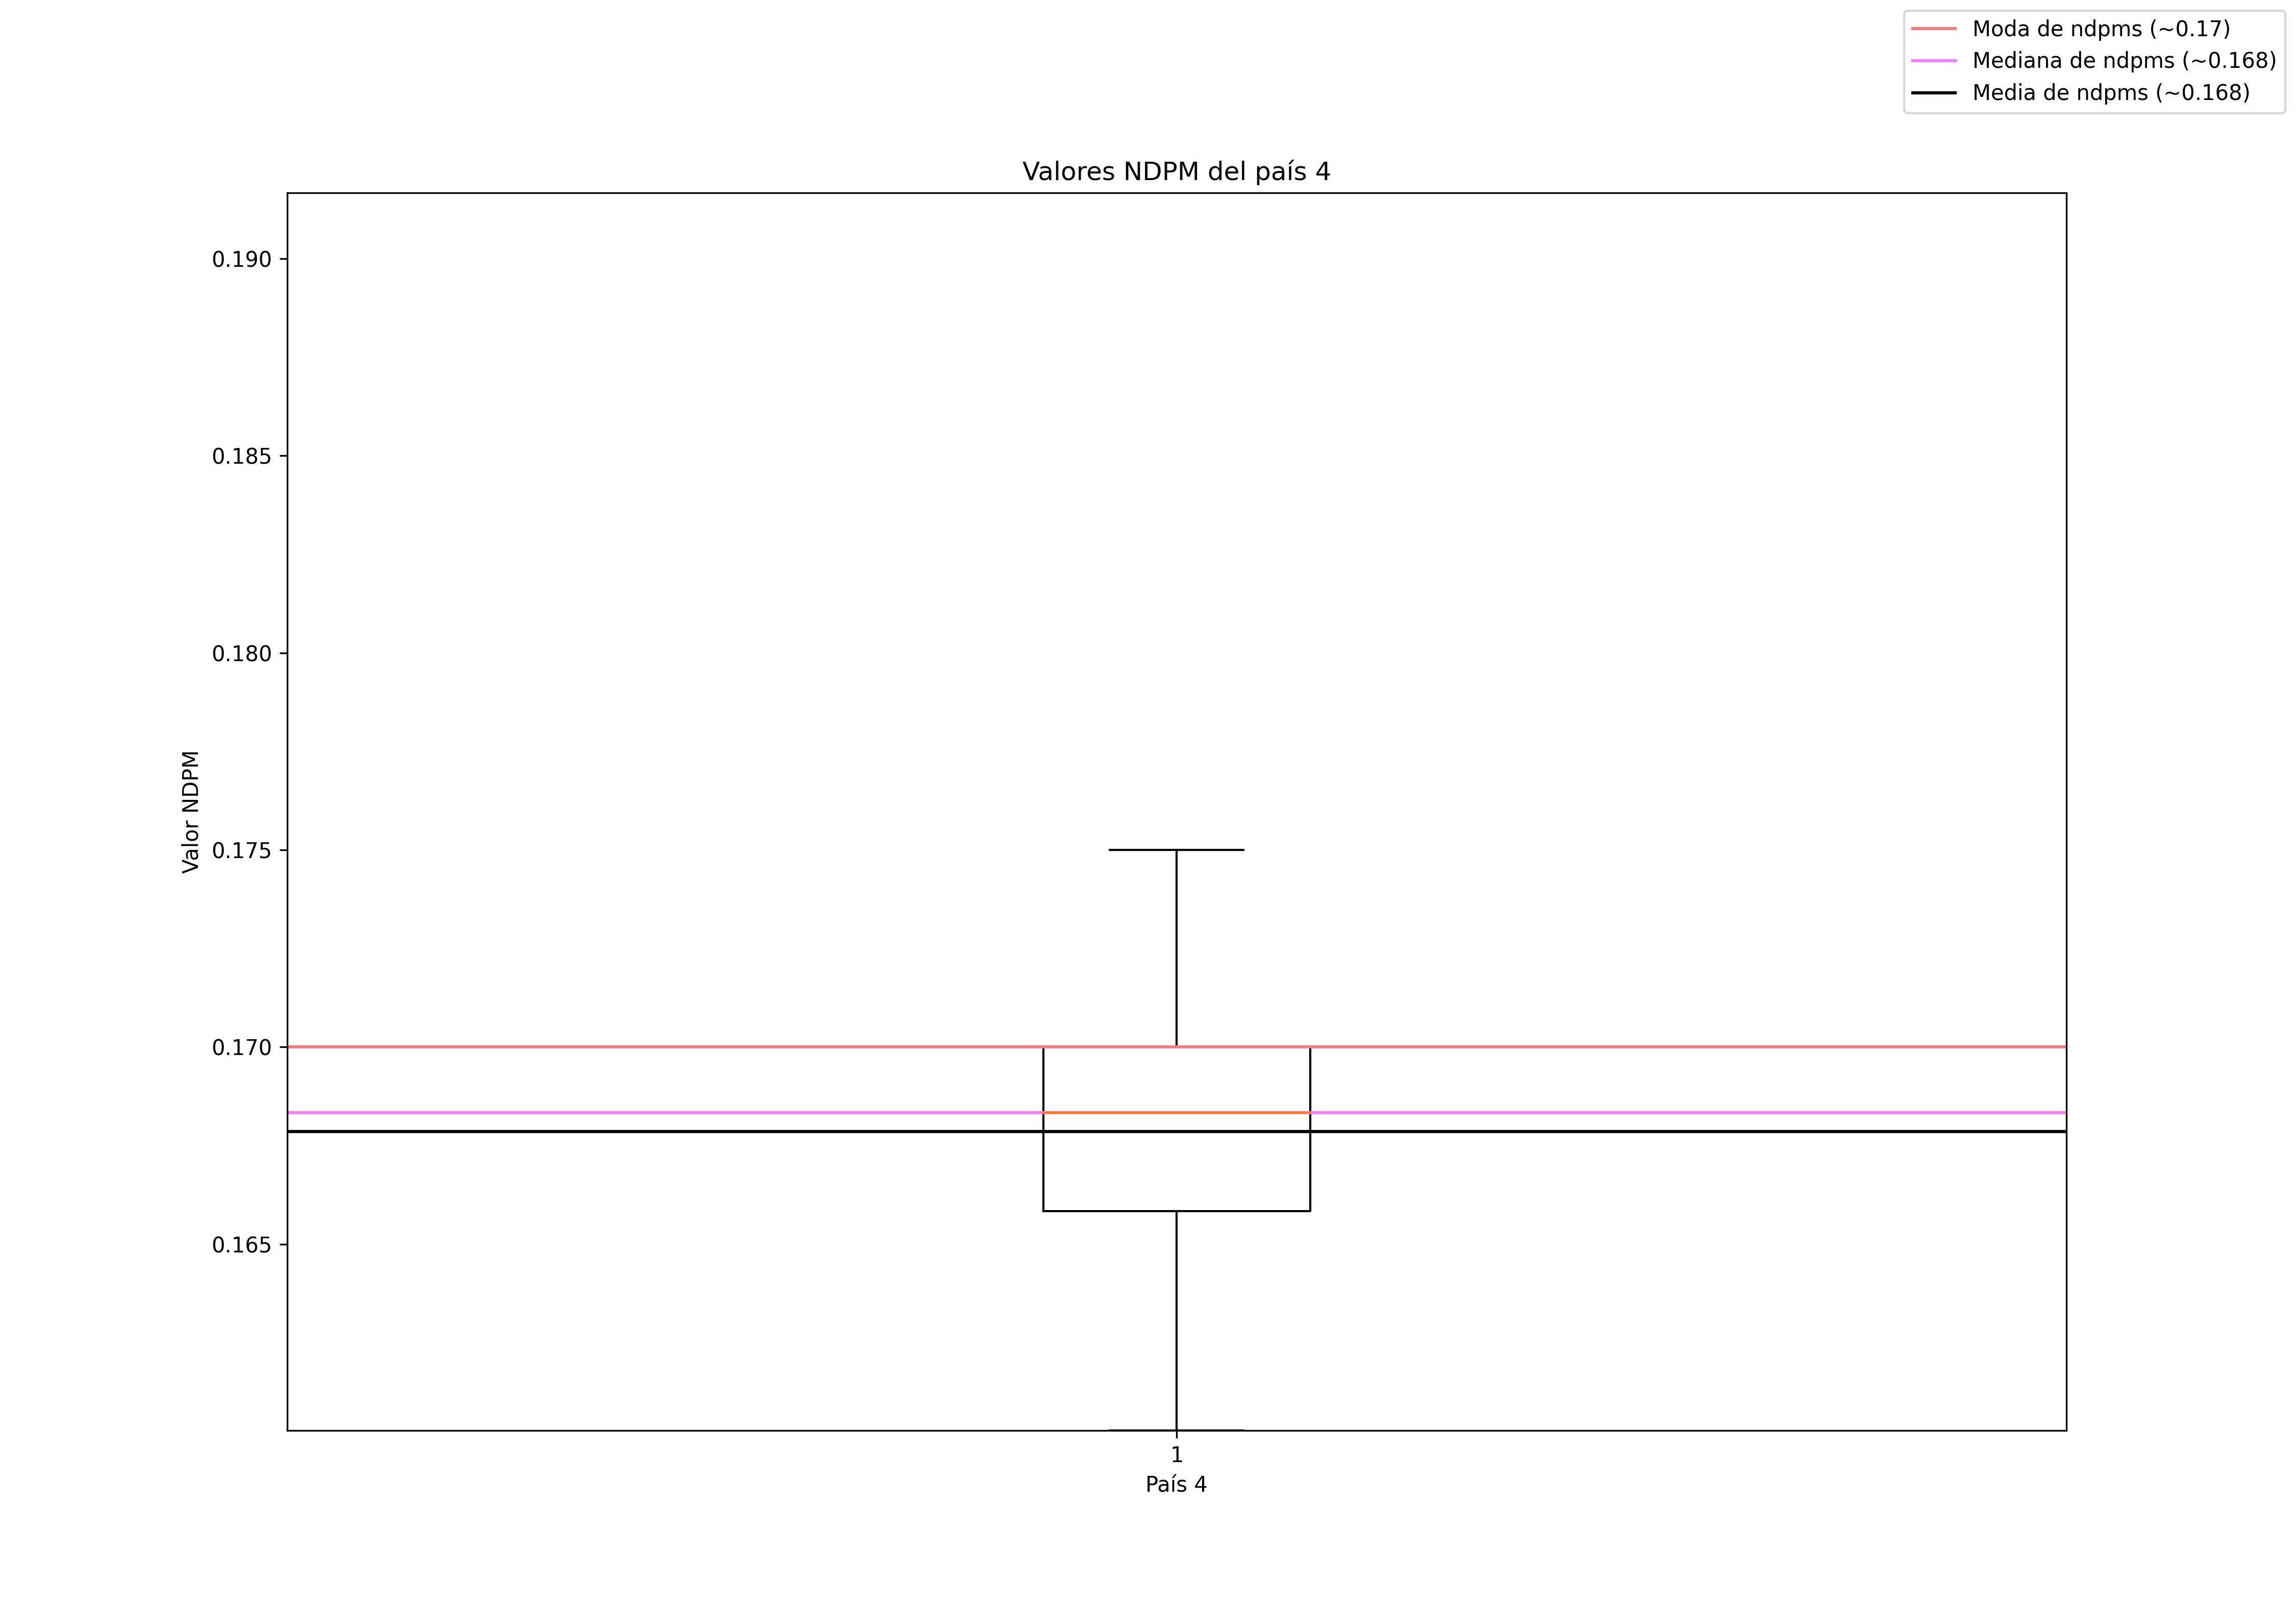
\includegraphics[width=0.5\textheight]
        {Figuras/Reports/PI_4_W1_EXT_CAJAS.png}}
    \caption{Diagramas de cajas y bigotes de los valores NDPM del participante 4\label{fig:PI4_CAJAS}}
\end{sidewaysfigure}
\clearpage
\begin{sidewaysfigure}
    \centering
    \subfloat[Modelo original]
        {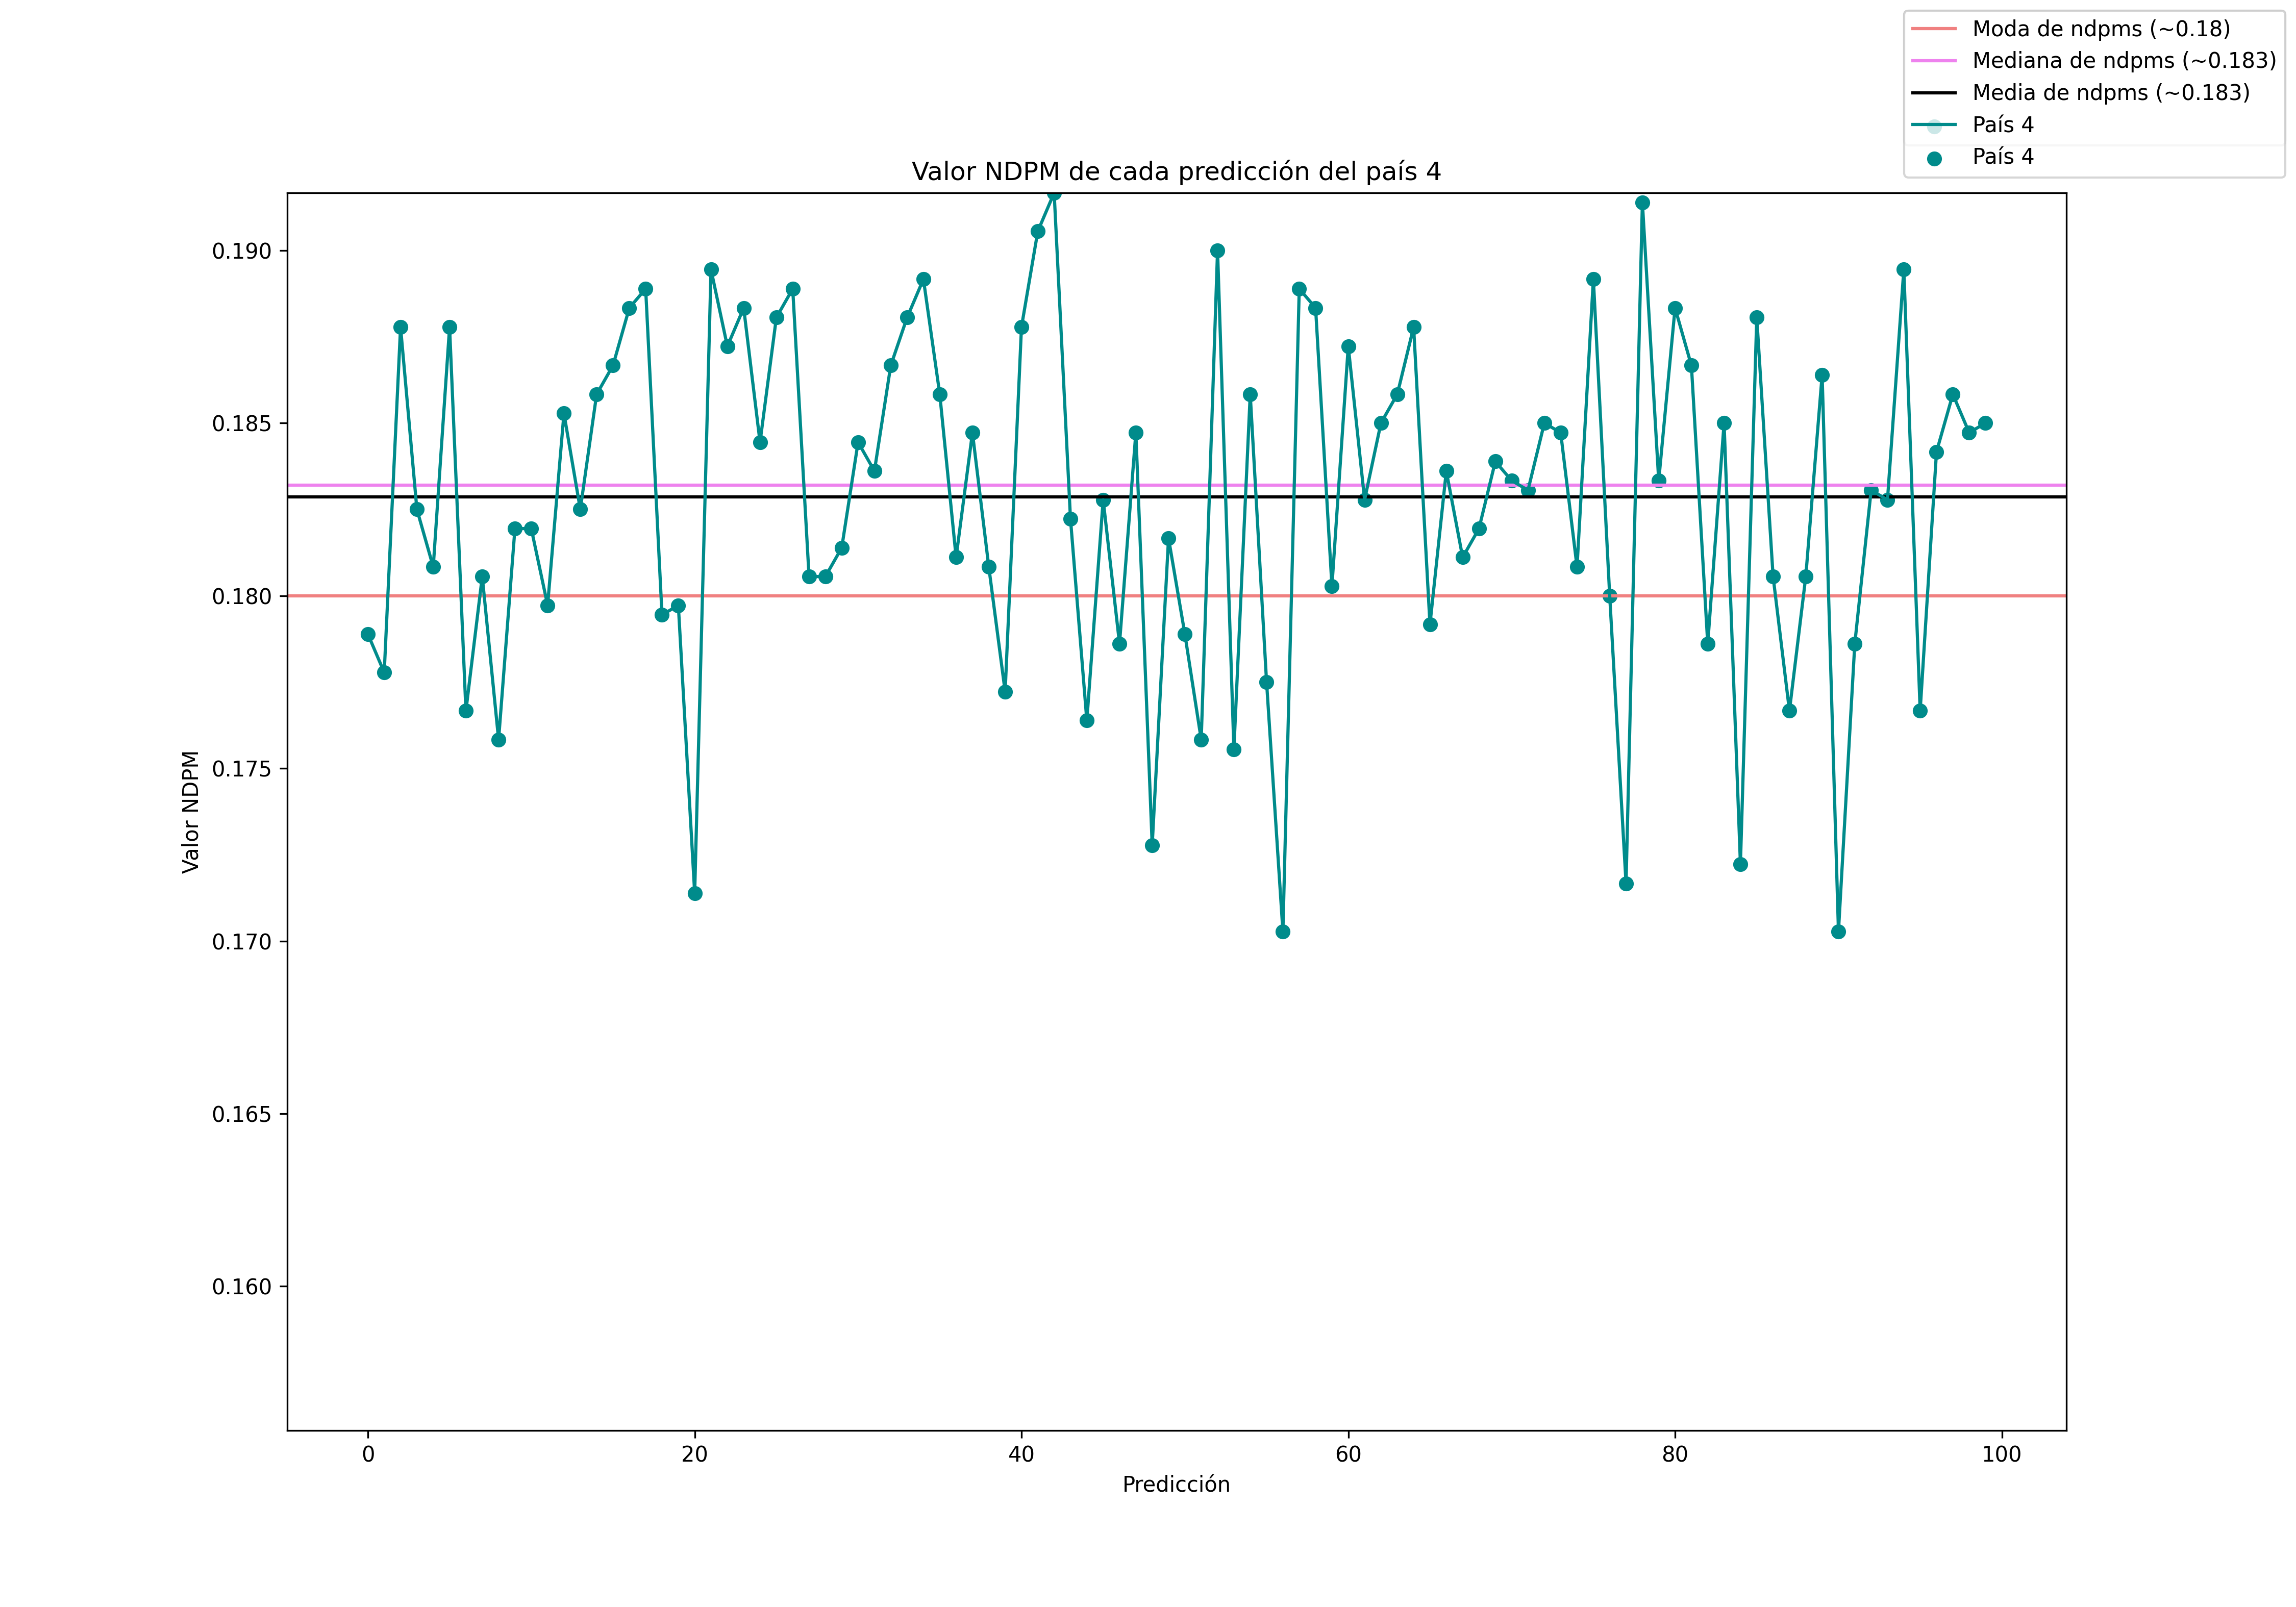
\includegraphics[width=0.5\textheight]
        {Figuras/Reports/PI_4_W0_LOC_DISP.png}}
        \quad
    \subfloat[Reentrenado con \textit{W$_c$ $=0$}]
        {\includegraphics[width=0.5\textheight]
        {Figuras/Reports/PI_4_W0_EXT_DISP.png}}
    \subfloat[Reentrenado con \textit{W$_c$ $=1$}]{
        \includegraphics[width=0.5\textheight]
        {Figuras/Reports/PI_4_W1_EXT_DISP.png}}
    \caption{Gráfico de los valores NDPM del participante 4\label{fig:PI4_DISP}}
\end{sidewaysfigure}
\clearpage




\subsubsection{Conclusiones}
Teniendo en cuenta lo anteriormente mencionado, podría decirse que este sistema permite que los participantes que cuentan con pocos datos se beneficien del conocimiento de otros usuarios, aunque estos no se vean compensados en ocasiones. Con cada iteración del protocolo el conocimiento pasa a ser más homogéneo a lo largo de los participantes. Además, con la introducción de nuevos datos en cada participante se consigue un sistema sostenible en el tiempo.
\\ \\
Las diferencias que plantea el FL sobre el ML convencional pueden resultar en ocasiones beneficiosas, en este caso, debido a la heterogeneidad de los datos, la segregación de modelos es beneficiosa. En ocasiones, cada grupo de usuarios necesita su propio modelo porque un modelo global les perjudica, como es el caso del participante 1 en la tabla \ref{tab:NDPM_PARTICIPANTE_1}. El caso es que el participante 1 en el sistema FL de información descentralizada es capaz de elaborar predicciones con más precisión que un RS con información centralizada, su participación en el sistema de FL permite que participantes que tendrían peores resultados que el RS convencional mejoren bastante su rendimiento. Esto se puede ver claramente en las tablas \ref{tab:NDPM_PARTICIPANTES_COLOR_W0} y \ref{tab:NDPM_PARTICIPANTES_COLOR_W1}, donde todos los participantes consiguen resultados mucho mejores que el RS convencional, siendo el participante 4 el único que se acerca al rendimiento del RS convencional por debajo. 
\\ \\
En este caso queda claro que la heterogeneidad de los RSs en ocasiones perjudica a un sistema centralizado y beneficia a un sistema distribuido. 
% \newpage
% \section{Tecnologías utilizadas}

\subsection{Sistema de recomendación}
El RS de R. Sánchez y col. utiliza LightFM\footnote{LightFM es una implementación en python de varios algoritmos populares de recomendación.} para crear los modelos de IA. Para implementar el FL se ha tenido que modificar gran parte del RS previo y se ha tenido que hacer uso de las utilidades que proporciona LightFM que se van a explicar en los siguientes apartados. 
\subsubsection{Creación del modelo}
El paso de creación del modelo es un paso complejo puesto que conlleva la correcta gestión de muchos datos e información. Asimismo, estos datos han de estar correctamente estructurados y construidos, puesto que LightFM requiere que la información este convertida a matrices dispersas y no tolera elementos vacíos en ellas. Para ello LightFM provee de herramientas de creación de datasets que facilitan la creación de las matrices, de forma que sea más fácil incluirlas en el modelo. 
\\ \\
Entre estas herramientas se encuentran:

\begin{itemize}
    \item \textit{build\_user\_features($\ldots$)} \quad Permite crear la matriz CSR de usuarios y atributos de usuarios.
    \item \textit{build\_item\_features($\ldots$)} \quad Permite crear la matriz CSR  de items y atributos de items.
    \item \textit{build\_interactions($\ldots$)} \quad Permite crear las matriz COO de interacciones y las matriz COO de sus correspondientes pesos.
\end{itemize}

Hay que tener en cuenta que las matrices CSR (Compressed Sparse Row) hacen referencia a las matrices que admiten operaciones matriciales y acceso eficientemente; y que las matrices COO (Coordinate list) hacen referencia a las matrices que soportan modificaciones eficientemente, son generalmente utilizadas para construir matrices.


\paragraph{Atributos de los usuario}
Para crear el modelo, es necesario entre otras cosas, disponer de las características de los usuarios. En este caso contamos con multitud de atributos sobre cada usuario (véase la tabla \ref{tab:AtributosUsuarios}).
\\ \\
Para convertir toda esa información del usuario a la matriz CSR que exige LightFM habrá que llamar a \textit{build\_user\_features($\ldots$)} con los IDs de usuario y sus atributos, formando una lista que tenga listas de los IDs de los usuarios con sus listas de atributos, es decir:

\begin{figure}[H]
    \centering
    \includegraphics[width=0.9\textwidth]{Figuras/LightFM_build_user_features.png}    
    \caption{Creación de la matriz de atributos de usuario} 
    \label{fig:BuildUserFeatures}
\end{figure}

\paragraph{Atributos de los elementos}
Además de los usuarios y de sus atributos, también se ha de disponer de los elementos a ordenar en el ranking, llamados items, y de sus características. En este caso estos items representan las estrategias de persuasión por las que se preguntó a los usuarios en el cuestionario. Sin embargo, al contrario que en el punto anterior, no contamos con tantos atributos sobre estos items, sino que cada estrategia de persuasión cuenta con dos atributos llamados dimensiones. Estos atributos no se encuentran presente en todas las estrategias, lo que da como resultado que haya algunas que tengan dos, una o ninguna dimension (véase la tabla \ref{tab:EstrategiasPersuasion}).
\\ \\
Para convertir toda esa información de los items a la matriz CSR que exige LightFM habrá que llamar a \textit{build\_item\_features($\ldots$)} con los IDs de las estrategias y y sus atributos, formando una lista que tenga listas de los IDs de las estrategias con sus listas de atributos, es decir:

\begin{figure}[H]
    \centering
    \includegraphics[width=0.9\textwidth]{Figuras/LightFM_build_item_features.png}    
    \caption{Creación de la matriz de atributos de los elementos} 
    \label{fig:BuildItemFeatures}
\end{figure}

\paragraph{Interacciones}
Para crear las interacciones de entrenamiento y de testeo LightFM nos facilita un método para poder crearlo fácilmente. Esta herramienta se utilizará dos veces como mínimo, una con los identificadores y atributos de los usuarios que serán utilizados para entrenar el modelo y la otra para generar las interacciones de los usuarios con los que se quiere realizar las predicciones.
\begin{figure}[H]
    \centering
    \includegraphics[width=0.9\textwidth]{Figuras/LightFM_build_interactions.png}    
    \caption{Creación de la matriz de interacciones} 
    \label{fig:BuildInteractions}
\end{figure}

\subsubsection{Ajuste}
Para permitir que el modelo pueda ser reajustado con nuevos datos y permitir el aprendizaje incremental LightFM implementa una variante de la herramienta \textit{fit($\cdots$)}. En un principio \textit{fit($\cdots$)} ajusta el modelo pero si se vuelve a utilizar esta herramienta se reajusta desde cero, sin mantener ningún dato insertado en el modelo antes.
\\ \\
Para solucionar esto LightFM tiene una variante llamada \textit{fit$\_$partial($\cdots$)}, esta herramienta permite ajustar datos al modelo tantas veces como se quiera sin perder los datos insertados previamente.
\begin{figure}[H]
    \centering
    \includegraphics[width=0.9\textwidth]{Figuras/LightFM_fit_partial.png}    
    \caption{Ajustar datos al modelo} 
    \label{fig:FitPartial}
\end{figure}

\subsubsection{Predicción}
Para generar las predicciones LightFM implementa un método que sintetiza el proceso y permite que insertando los interacciones de test se prediga el ranking para estos usuarios.
\begin{figure}[H]
    \centering
    \includegraphics[width=0.9\textwidth]{Figuras/LightFM_predict_rank.png}    
    \caption{Ajustar datos al modelo} 
    \label{fig:FitPartial}
\end{figure}
\subsubsection{Evaluación}
La evaluación de los resultados obtenidos de las predicciones de los modelos es un apartado fundamental que permite analizar la eficacia de estas predicciones. Además, la utilización de métricas y técnicas permitirá poder comparar los resultados entre sí para poder demostrar si la predicción es correcta, aceptable o errónea.
\\ \\
Para este caso no se incluirá ninguna métrica ni método de LightFM, sino que se utilizará la métrica NDPM implementada y explicada en el apartado de valoración \ref{Valoracion}.


\subsection{Memoria}
La memoria técnica de este proyecto ha sido elaborada en \LaTeX. Esta ha sido escrita en el editor de código \textit{Visual Studio Code} gracias al complemento \textit{LaTeX Workshop}, que proporciona las características básicas para la composición tipográfica de \LaTeX $ $ en \textit{Visual Studio Code}, y gracias a \textit{MiKTeX}, distribución Tex para Windows, la cual permite la compilación de documentos \LaTeX $ $ en Windows.
\\ \\
Además, para controlar el avance y las versiones de la memoria se ha utilizado el controlador de versiones GIT. Para que las versiones no permaneciesen en el ordenador local se decidió abrir un repositorio en GitHub\footnote{Repositorio: $https://github.com/Ibaii99/PFG\_MEMORIA$} donde se ha ido desarrollando este proyecto.
\\ \\
Para la gestión bibliográfica se ha utilizado \textit{Zotero}, herramienta que permite gestionar las citas bibliográficas a través de una app y un complemento en el navegador. Para exportar estas referencias a \LaTeX $ $ se ha utilizado el paquete \textit{BibTex}.
\subsection{Desarrollo}
El desarrollo de este proyecto se ha realizado en el editor \textit{Visual Studio Code} y con el leguaje de programación \textit{Python}, al igual que la memoria se ha utilizado el controlador de versiones GIT con un repositorio en Github. A lo largo del desarrollo del proyecto han surgido diferentes necesidades que se han ido solucionando con la incorporación de ciertas herramientas, estas herramientas han sido agrupadas en función de las necesidades que han solventado en el proyecto, se detallan a continuación.
\subsubsection{Matrices}
A la hora de gestionar matrices de grandes dimensiones se ha utilizado la biblioteca \textit{NumPy}, la cual da soporte para crear grandes matrices multidimensionales y realizar operaciones matemáticas de alto nivel con ellas. 
\\ \\
Se han usado matrices NumPy tanto para la gestión de la información y estructurar los datos en LightFM como para realizar las tareas del modelo de consenso.
\subsubsection{Cálculos estadísticos} 
A la hora de realizar los cálculos sobre las matrices de predicción en el modelo de consenso la mediana y moda han tenido que ser aplicadas con distintas librerías. Aunque se ha intentado utilizar \textit{NumPy} para todo esta biblioteca no contaba con ningún método que permitiera calcular la moda de una lista, por lo cual ha habido que importar una biblioteca extra, \textit{SciPy}.
\\ \\
\textit{SciPy} permite aplicar bastantes algorítmos y herramientas matemáticas, pero solo se ha importado su paquete de funciones estádisticas \textit{stats}. 
\subsubsection{Guardado de los modelos}
Uno de los principales problemas del proyecto era el envío de los modelos y para ello se necesitaba exportar el modelo a un fichero para poder enviarlo por la red. Como LightFM permite la serialización de sus modelos se elijió la biblioteca \textit{pickle} para este proceso. Esta biblioteca implementa módulos binarios para la serialización y deserialización, por lo cual permitia tanto guardar a fichero el modelo como importarlo desde un fichero.
\subsubsection{Securización} 
Para la implementación de la seguridad en las comunicaciones y realizar las operaciones criptográficas se ha utilizado el paquete \textit{cryptography}, este paquete provee de métodos de cifrado y descifrado simétricos y asimétricos de alto nivel, lo que permite un nivel de abstracción mayor y por ende una más fácil gestión. 
\subsubsection{Compresión}
Un elemento fundamental del proyecto era minimizar el volumen de las comunicaciones puesto que es uno de los grandes inconvenientes del FL. Con el objetivo de minimizar el tamaño de las comunicaciones se identificaron donde se daban los mayores volúmenes de conexión y se averiguó que era en el intercambio de modelos entre los participantes y el servidor y viceversa. Para ello la compresión de las comunicaciones se realizó mediante la biblioteca \textit{zlib}. 
\subsubsection{Gestión de la ejecución}
Como en este proyecto se gestionan muchos dispositivos y se tiene que reproducir en protocolo de FL en orden es crucial poder controlar lo que se ejecuta en cada dispositivo. Para poder gestionarlo con más facilidad se ha implementado el paquete \textit{OptionParser} para poder definir ciertos \textit{flags} para especificar qué proceso se quiere ejecutar en el dispositivo.
\\ \\
En cuanto a los flags generales se encuentran:
\begin{itemize}
    \item \textit{-k}, para generar las claves públicas y privadas de encriptación.
    \item \textit{-e}, para encriptar los modelos con la clave pública del receptor.
    \item \textit{-d}, para desencriptar el modelo recibido con la clave privada propia.
\end{itemize}   
Sin embargo, debido al funcionamiento dispar del nodo respecto a los participantes hay diferentes \textit{flags} dependiendo del dispositivo, de esta forma las Raspberries cuentan con:
\begin{itemize}
    \item \textit{-t}, para generar un modelo LightFM y entrenarlo con los datos del país.
    \item \textit{-c}, para comparar el modelo reentrenado recibido con el que tiene el dispositivo.
    \item \textit{-v}, para realizar el entrenado del modelo y la encriptación.
    \item \textit{-w}, para desencriptar el modelo reentrenado y compararlo con el local.
    \item \textit{-a}, flag extra solo usado en desarrollo que permite simular virtualmente a los participantes, su única utilidad ha sido durante el desarrollo y no durante el RS.
\end{itemize}
A su vez, el nodo de agregación ha tenido también sus diferentes tareas:
\begin{itemize}
    \item \textit{-s}, para generar los datos sintéticos.
    \item \textit{-c}, consensuar los datos sintéticos con los modelos de los participantes.
    \item \textit{-v}, desencriptar el modelo del participante, generar los datos sintéticos, realizar el consenso de los datos y encriptar los modelos reentrenados.
\end{itemize}
\begin{figure}[H]
    \centering
    \includegraphics[width=0.8\textwidth]{Figuras/Raspberry_procedure_h.png}
    \caption{Opciones de ejecución de las Raspberries} 

    \includegraphics[width=0.8\textwidth]{Figuras/jetsonnano_procedure_h.png}
    \caption{Opciones de ejecución de la Jetson Nano} 
\end{figure}


\subsubsection{Aprovisionamiento}
Uno de los riesgos del proyecto que se ha incluido en la sección de gestión de riesgos ha sido la creación de un \textit{script} que permita automatizar la instalación de todos los paquetes necesarios para la ejecución del proyecto en caso de que una tarjeta SD se averiase.
\\ \\
Los \textit{script}s que se han desarrollado para cumplir con este objetivo han sido dos, uno de aprovisionamiento del sistema linux y otro de requisitos de paquetes python. En un proyecto normal hubiera valido con un simple script de requisitos de python \textit{requirements.txt} el cual alberga el nombre de los paquetes y la versión a instalar, proceso fácilmente realizable mediante el comando \textit{pip install -r requirements.txt}. Sin embargo, en este proyecto los paquetes que se utilizan no son fácilmente importables de un sistema operativo a otro, por lo que ha habido que desarrollar un pequeño script de aprovisionamiento en \textit{bash} que mediante consola instalase todos los paquetes necesario para el correcto funcionamiento de los paquetes python en las Raspberries y la Jetson Nano.
\\ \\
Cada tipo de dispositivo ha tenido su propio conjunto de ficheros de aprovisionamiento, de forma que ha habido un \textit{requirements.txt} y un script en \textit{bash} para las Raspberries y otro para la Jetson nano, ya que por sistema operativo, arquitectura y compatibilidades los dispositivos deben funcionar con distintas versiones de ciertos paquetes y en caso de las Raspberries con algún paquete más.

\subsubsection{Reporte de resultados}
Con el objetivo de representar los resultados de la precisión de los rankings de una forma vistosa y fácilmente entendible se incorporó la biblioteca \textit{Matplotlib} para la generación de gráficos. Esta biblioteca permite crear diversidad de gráficos para representar la información, elemento imprescindible a la hora de comparar el rendimiento del sistema.

\subsection{Sistemas operativos}
En cuanto a sistemas operativos se ha trabajado tanto con \textit{Windows} a la hora de realizar el desarrollo como con \textit{Linux} a la hora de realizar la implementación. Los sistemas \textit{Linux} que se han utilizado han sido \textit{RaspbianOS}, sistema operativo derivado de \textit{Debian} para las Raspberries con soporte oficial, y una adaptación de \textit{Ubuntu} para la Jetson Nano.
\subsection{Comunicaciones}
Como bien se ha explicado en el apartado de securización de las comunicaciones \ref{SegCom} para comunicarse con los dispositivos y poder parametrizarlos y configurar la instalación se utilizará el protocolo \textit{SSH}, el cual permite abrir una línea de comando desde un dispositivo a otro.
\\ \\
Además, para el intercambio de ficheros se ha utilizado el protocolo \textit{SCP}, el cual se apoya en gran parte del protocolo \textit{SSH} y al igual que este está explicado en el apartado de securización de las comunicaciones \ref{SegCom}.
% \newpage
% \section{Consideraciones sobre la implementación}
En este capítulo se describirán tanto las causas que han llevado a adoptar la previa especificación del diseño del sistema, como las razones detrás de ellas. Con el objetivo de ayudar a entender el por qué de las decisiones tomadas se hablará sobre la privacidad, seguridad, la combinación de los modelos y las limitaciones técnicas presentes en este proyecto.
\subsection{Privacidad}
Con el objetivo de no vulnerar la privacidad de los datos, la agregación de los modelos será realizada por consenso sobre usuarios sintéticos. De esta forma, se evitan problemas derivados del robo de datos y las consecuencias tanto legales como personales de este.
\\ \\
Partiendo del principio de que si no circula ningún dato de ningún usuario por la red no se corren tantos riesgos, se plantea este sistema de agregación como una alternativa viable a los sistemas tradicionales de ensamblado.

\subsection{Seguridad}
Este sistema está expuesto a los ataques de seguridad derivados de la implementación del FL. Sin embargo, debido a la naturaleza del algoritmo de consenso, algunos ataques podrían ser minimizados o incluso erradicados.
\\ \\
Un ejemplo de ello es el ataque por envenenamiento. Existen dos tipos de envenenamiento, por datos y por modelo. Ambos consisten en que un participante de la red, con el objetivo de dañar tanto al sistema como a los participantes, envía modelos de IA (o los datos si es por envenenamiento de datos) debidamente manipulados. En los sistemas de agregación de modelos de IA por ensamblado este tipo de ataque suele ser bastante dañino, ya que es capaz de distorsionar por completo los resultados del modelo final con lo recibido del atacante.
\\ \\
Sin embargo, debido a la condición del sistema de agregación por consenso, este tipo de ataques no son tan efectivos, ya que el modelo con datos envenenados podría ser ignorado si el método por el que se realiza el consenso es la moda. Con la moda se elegiría el ranking en función de los valores más frecuentes, es decir, el modelo del atacante sería ignorado por presentar predicciones que no se ajustan a ninguno de los demás participantes.
\\ \\
Cabe destacar que con el objetivo de detectar ataques y encontrar posibles modelos maliciosos, se podrían descartar del proceso todos aquellos modelos que presenten unas predicciones totalmente diferentes. Se podría analizar la varianza de las predicciones de cada modelo para descartar del proceso a presuntos modelos envenenados.

\subsection{Combinación de modelos}
Debido a que el principal objetivo de este proyecto es el desarrollo de un RS basado en FL con la privacidad como patrón de diseño, la combinación de los diferentes modelos de los participantes ha sido un factor muy importante a tener en cuenta. En el ML tradicional esta agregación de modelos se producía mediante el ensamblado de modelos. Sin embargo, este proceso no es compatible con este proyecto puesto que para poder ensamblar los modelos habría que compartir información de los participantes de la red.
\\ \\
Para evitar compartir ningún tipo de información que comprometiese la seguridad y privacidad de los participantes de la red de FL pero conseguir que los participantes aprendiesen entre ellos, se optó por compartir los modelos de IA exclusivamente.
\\\\
Además, el uso del modelo de consenso permite que se pueda usar cualquier framework o librería para desarrollar los modelos de IA, permitiendo que se pudieran implementar este tipo de redes sin necesidad de usar exclusivamente las librerías que tienen incorporados los métodos para el FL.

\subsection{Limitaciones técnicas}
Debido a que los dispositivos que iban a formar la red iban a ser 4 Raspberries Pi modelo 3b+, el procesado de los datos era un proceso de especial importancia por la \textit{escasa} capacidad de cómputo de estos dispositivos. Estos dispositivos, como se puede ver en el capítulo de especificación del diseño, son dispositivos que tienen cuatro núcleos y 1.4GHz de frecuencia, lo que comparado con un ordenador de sobremesa actual supone una gran diferencia de potencia de cálculo.
\\ \\
Además, esa no es la única diferencia que tienen respecto a los ordenadores de escritorio, las Raspberries Pi funcionan sobre arquitectura ARMv8 y no sobre las tan usadas x64 y x86 . Esto implica un gran problema a la hora de instalar los paquetes necesarios para que el proyecto sea ejecutable en estos dispositivos, ya que la mayoría de los paquetes necesarios están pensados para las arquitecturas más comunes (x64 y x86). Sin embargo, se han podido encontrar las versiones funcionales de todos los paquetes para estos dispositivos.
\\ \\
El dispositivo que iba a agregar los datos, la Nvidia Jetson Nano, ha sido más sencilla de configurar puesto que esta funciona sobre arquitectura AArch64, extensión de 64bits de la arquitectura ARM.

% \newpage
% \section{Retos abordados en el proyecto}
El FL es una tecnología nueva que cuenta con muchas vías de investigación, el objetivo de esta sección es explicar las vías abiertas que se han estudiado y abordado. 
\subsection{Convergencia del algoritmo de aprendizaje}
Una de las consideraciones principales del FL es la convergencia de los distintos modelos. Se trata de optimizar los modelos, minimizando los datos que se suben a estos. No obstante, la convergencia no está siempre garantizada, pero ya se cuenta con proyectos dedicados a lograr la plena convergencia del modelo global.
\\ \\
Este proyecto trata de abordar este reto desde otro punto de vista, en vez de intentar combinar los algoritmos para tratar de que estos compartan el conocimiento a través de usuarios sintéticos como se ha explicado anteriormente. Esta solución, además, permite que este enfoque se pueda aplicar a cualquier caso de uso debido a que no tiene dependencias respecto al framework de IA que se esté usando. Los algoritmos clásicos de FedAvg y FedSGD están implementados en Tensorflow, pero si se quisieran usar en otro sistema habría que desarrollarlos o buscar alguna solución ajena al framework, mientras que el algoritmo de consenso es un sistema que permite converger los resultados de una matriz de predicciones en una simple lista. Que a su vez esta lista será usada para reentrenar a los participantes y mejorar su precisión. Concepto que puede ser aplicado a multitud de RSs.

\subsection{Privacidad}
El reto de la privacidad es cada vez más relevante en un mundo donde todo está cada vez más digitalizado. El FL cuenta con la privacidad como una de sus principales ventajas, pudiendo utilizar el modelo de aprendizaje de manera local, intercambiando únicamente los parámetros necesarios con el modelo global alojado en el servidor. 
\\ \\
No obstante, un atacante puede obtener acceso a cierta información confidencial si logra acceder al modelo global. Para cubrir esta carencia, se proponen diferentes soluciones en las que se sacrifica algo de rendimiento con el fin de lograr la plena seguridad, y se está logrando un equilibrio mayor con el paso del tiempo.
\\ \\
Este reto ha sido solucionado mediante el enfoque de reentrenado en vez de el clásico enfoque de converger los modelos. Esto quiere decir que, en este caso, los modelos no se \textit{``fusiona''}, sino que cada uno se reentrena con datos sintéticos para los cuales se ha estimado un resultado a través del método de consenso. De esta forma, se evita que un participante albergue en su modelo información de otro participante y podrá evitar que su información esté en los dispositivos de otros.

\subsection{Seguridad en la comunicación}
Un reto al que se ha tenido que enfrentar el FL ha sido la exposición a ciberataques, principalmente mediante interferencias o DoS. El ataque por interferencias consiste en enviar señales de alta frecuencia para generar interferencias en las comunicaciones entre los dispositivos móviles y el servidor, algo que provoca errores en los datos transferidos entre los clientes y el servidor, y que reduce de forma drástica el rendimiento del modelo. 
\\ \\
Sin embargo, este reto se puede abordar de manera exitosa enviando copias del modelo a través de diferentes frecuencias para reducir el riesgo de que el modelo se corrompa de algún modo.
\\ \\
En este proyecto la seguridad de la comunicación ha sido un punto fundamental, ya que todas las comunicaciones están cifradas con cifrado híbrido, y en caso de que un participante no recibiese su modelo por desconexión podría pedirlo de nuevo al nodo principal. Sin embargo, no se ha tenido en cuenta la conexión inalámbrica ni los ataques de denegación de servicio, esto sería un nuevo campo a estudiar y no quedaría resuelto del todo.  

\subsection{Combinación de algoritmos de reducción de comunicaciones}
Actualmente, hay tres técnicas de reducción de comunicaciones en FL, cuya combinación puede resultar realmente efectiva a la hora de reducir el tamaño de los datos intercambiados con el modelo global. Por ahora, se están desarrollando técnicas que permitan una buena combinación de estos algoritmos con la finalidad de maximizar la eficiencia del sistema global de FL.
\\ \\
Con el objetivo de maximizar la eficiencia de las comunicaciones se han implementado mecanismo de compresión de los bytes del modelo y de la información a enviar por la red, reduciendo con zlib considerablemente el tamaño de los mensajes.


% \newpage
% \section{Incidencias ocurridas}
Durante el desarrollo del proyecto ocurrieron varios problemas con los dispositivos implicados que se han decidido mencionar. 
\\ \\
En el principio del desarrollo del proyecto se optó por la utilización de otro modelo de Raspberries, menos potentes y más antiguas, que eran incompatibles con las versiones de los paquetes que había que utilizar. Tras muchas pruebas y después de intentar compilar uno a uno cada paquete para el dispositivo se decidió desistir y cambiarlos por las actuales Raspberry Pi 3B +, mucho más actuales.
\\ \\
Al realizar el cambio de los cuatro dispositivos y tener que reconfigurar todas las tarjetas sd se perdió gran parte del tiempo, puesto que las primeras fases de la configuración han de realizarse con la Raspberry conectada a una pantalla con teclado y ratón para habilitar los diferentes protocolos de comunicación. Una vez con esta configuración, se ejecutaron los \textit{script}s de aprovisionamiento preparados para reinstalar todos los paquetes, lo que permitió que el proceso no se alargara mucho más. 
\\ \\
Cuando parecía que todo estaba solucionado una Raspberry falló y se rompió, lo que provocó que hubiera que desmontar todo el rack \ref{fig:RackRaspberry} y poner una Raspberry nueva. Este proceso al tratarse únicamente de hardware y al intercambiarse por el mismo modelo no trajo mayores problemas puesto que se podía utilizar la misma tarjeta SD con la misma configuración.

% \fancyhead[LE]{}
% \newpage
% \thispagestyle{empty}
% \cleardoublepage


% \chapter{Presupuesto}
\thispagestyle{fancy}
\fancyhead[LE]{\thechapter.Presupuesto} 
El presupuesto de este proyecto cuenta con dos apartados, el presupuesto de los materiales y el de los recursos humanos. Adicionalmente se ha añadido un apartado para explicar los requisitos de la plataforma de desarrollo, que al no ser adquirida para este proyecto no entra dentro de los costes, pero es un elemento fundamental para el desarrollo de software en este proyecto. 

\section{Plataforma de desarrollo}
Aunque el proyecto conste únicamente del gasto en materiales y recursos humanos se ha utilizado un ordenador de escritorio para su desarrollo. Aunque el presupuesto de este ordenador no sea exclusivo para el proyecto ha sido necesario para su desarrollo y para agilizar los despliegues y las pruebas. Además, este ordenador ha sido utilizado para desarrollar el código y probarlo, actividad que también ha agilizado mucho el desarrollo del proyecto.
\\ \\
Es por esto que, aunque no entre en el presupuesto, merecía ser mencionado. El ordenador cuenta con los diferentes componentes, tabla \ref{tab:PlataformaDesarrollo}.

\begin{table}[H]
    \begin{center}
    %Se centra la tabla.
        \begin{tabular}{|c|}
            % -------------
            \hline
            \rowcolor{Cyan} 
            \textbf{Plataforma de desarrollo} \\ 
            % -------------
            \hline
            \rowcolor{GrisTabla}
            \textbf{Ordenador de torre} \\
            \hline
            GPU: Nvidia GTX 970 \\
            \hline
            CPU: Ryzen 5 3600 \\
            \hline
            RAM: 16 gb \\
            % -------------
            \hline
        \end{tabular}
        \caption{\centering Presupuesto de los materiales utilizados.}
        \label{tab:PlataformaDesarrollo}
    \end{center}    
\end{table}


\newpage
\section{Materiales}
En cuanto al presupuesto de los materiales que se han utilizado en el proyecto, se ha elaborado la tabla \ref{tab:PresupuestoMateriales} donde se detalla tanto la lista de materiales, como su precio.
\\ \\
Este presupuesto está agrupado en 5 categorías, las Raspberries Pi, las tarjetas SD, la Jetson Nano, los cables y los elementos de telecomunicación. Esta clasificación permite observar en qué grupos se ha gastado más. 

\begin{table}[H]
    \begin{center}
    %Se centra la tabla.
        \begin{tabular}{|r|c|r|r|}
            % -------------
            \hline
            \rowcolor{Cyan} 
            % -------------
            \multicolumn{4}{|c|}{\textbf{Materiales}}\\
            \hline
            \textbf{Hardware} & \textbf{Cantidad} & \textbf{Precio unidad}& \textbf{Precio total}\\ 
            % -------------
            \hline
            \rowcolor{GrisTabla}
            \textbf{Raspberries} &  \textbf{5} & & \textbf{185,40 \euro}\\
            Pi 3 B & 1 & 37,44 \euro & 37,44 \euro\\
            Pi 3 B+ & 4 & 36,99 \euro & 147,96 \euro\\
            % -------------
            \hline
            \rowcolor{GrisTabla}
            \textbf{SD-s} &  \textbf{8} & & \textbf{50 \euro}\\
            16 GB & 1 & 6 \euro & 42 \euro\\
            32 GB & 4 & 8 \euro & 8 \euro\\
            % -------------
            \hline
            \rowcolor{GrisTabla}
            \textbf{Jetson Nano} & \textbf{1} & & \textbf{140 \euro}\\
            NVIDIA Jetson Nano & 1 & 140 \euro & 140 \euro\\
            % -------------
            \hline
            \rowcolor{GrisTabla}
            \textbf{Cables} &  \textbf{5} & & \textbf{137 \euro}\\
            Alimentación Raspberry & 5 & 10 \euro & 50\euro\\
            Alimentación Jetson Nano & 1 & 15 \euro & 15 \euro\\
            Regleta enchufes & 2 & 10 \euro & 10 \euro\\
            Rack Raspberries & 1 & 20 \euro & 20 \euro\\
            RJ45 & 8 & 4 \euro & 32 \euro\\
            % -------------
            \hline
            \rowcolor{GrisTabla}
            \textbf{Telecomunicaciones} &  \textbf{2} & & \textbf{29,41} \euro\\
            Switch & 1 & 11 \euro & 11 \euro\\
            Router & 1 & 18,41 \euro & 18,41 \euro\\
            % -------------
            \hline
            \rowcolor{Naranja} 
            % -------------
            \multicolumn{3}{|r}{\textbf{Total}} & \textbf{541,81 \euro}\\
            \hline
            % \rowcolor{Naranja} 
            % \textbf{V} & \textbf{elit} \\ \hline
        \end{tabular}
        \caption{\centering Presupuesto de los materiales utilizados.}
        \label{tab:PresupuestoMateriales}
    \end{center}    
\end{table}


\newpage
\section{Recursos Humanos}
En cuanto a los recursos humanos que intervienen en el proyecto se ha decidido contar con los siguientes tipos de especialistas que, desempeñando estos roles, desarrollarán el proyecto.

\begin{table}[H]
    \begin{center}
    %Se centra la tabla.
        \begin{tabular}{|l|c|p{0.4\linewidth}|}
            % -------------
            \hline
            \rowcolor{Cyan} 
            \textbf{Perfiles} & \textbf{Precio hora} & \textbf{Responsabilidades} \\ 
            % -------------
            \hline
            \rowcolor{GrisTabla}
            & & $\bullet$ Organización\\
            \rowcolor{GrisTabla}
            & & $\bullet$ Gestión\\
            \rowcolor{GrisTabla}
            & & $\bullet$ Delimitar alcance y objetivos\\
            \rowcolor{GrisTabla}
            \multirow{-4}{*}{\textbf{Jefe de proyecto}} & \multirow{-4}{*}{\textbf{45 \euro}} & $\bullet$ Búsqueda de tecnologías\\
            \hline

            & & $\bullet$ Realización de la memoria técnica\\
            & & $\bullet$ Preparación de la defensa\\
            & & $\bullet$ Entre e impresión de la memoria y defensa\\
            \multirow{-4}{*}{\textbf{Analista de software interno}} & \multirow{-4}{*}{\textbf{30 \euro}} & $\bullet$ Búsqueda de nuevas tecnologías\\
            \hline

            \rowcolor{GrisTabla}
            & & $\bullet$ Ideas sobre cómo afrontar problemas\\
            \rowcolor{GrisTabla}
            & & $\bullet$ Resolver dudas\\
            \rowcolor{GrisTabla}
            & & $\bullet$ Presentar sistema de recomendación anterior\\
            \rowcolor{GrisTabla}
            \multirow{-4}{*}{\textbf{Analista de software externo}} & \multirow{-4}{*}{\textbf{30 \euro}} & $\bullet$ Consejos\\
            \hline

            & & $\bullet$ Idear la estructura del modelo de consenso\\
            & & $\bullet$ Desarrollar el protocolo de federated learning\\
            \multirow{-3}{*}{\textbf{Arquitecto de software}} & \multirow{-3}{*}{\textbf{45 \euro}} & $\bullet$ Planificar conexiones entre dispositivos y requisito\\
            \hline

                
            % -------------
            \rowcolor{GrisTabla}
            \textbf{Desarrollador de software} & \textbf{35 \euro} & $\bullet$  Programación del proyecto\\
            \hline

            & & $\bullet$ Revisar gramática de la memoria\\
            & & $\bullet$ Revisar el software desarrollado\\
            \multirow{-3}{*}{\textbf{Gestor de calidad}} & \multirow{-3}{*}{\textbf{30 \euro}} & $\bullet$ Revisión de bugs y errores\\
            \hline

        \end{tabular}
        \caption{\centering Precio hora de los distintos perfiles que intervienen en el proyecto.}
        \label{tab:PrecioPerfil}
    \end{center}    
\end{table}
\pagebreak
Estos roles de la tabla \ref{tab:PrecioPerfil} serán interpretados por los siguientes colaboradores del proyecto, presentes en la tabla \ref{tab:PersonaPerfil}. Cabe destacar que el rol de analista interno solo será llevado a cabo por Ibai Guillén, el resto de participantes, en caso de desempeñarlo, ejercerán de analistas externos.
\begin{table}[H]
    \begin{center}
        %Se centra la tabla.
        \begin{adjustbox}{angle=90}  
                \begin{tabular}{|p{0.22\linewidth}|p{0.12\linewidth}|p{0.12\linewidth}|p{0.15\linewidth}|p{0.19\linewidth}|p{0.135\linewidth}|}
                    % -------------
                    \hline
                    \rowcolor{Cyan} 
                    \backslashbox{Personas}{Perfiles} & \textbf{Jefe de proyecto} & \textbf{Analista} & \textbf{Arquitecto} & \textbf{Desarrollador} & \textbf{Gestor de calidad}\\ 
                    % -------------
                    \hline
                    \rowcolor{GrisTabla}
                    \textbf{Oihane Gómez} &  & 2 horas &  &  & \\
                    % -------------
                    \hline
                    \textbf{Rubén Sánchez} &  & 3 horas &  &  & \\
                    % -------------
                    \hline
                    \rowcolor{GrisTabla}
                    \textbf{Diego Casado} & 6 horas & 8 horas & 6 horas &  & 4 horas\\
                    % -------------
                    \hline
                    \textbf{Ibai Guillén} & 40 horas & 100 horas & 50 horas & 110 horas & 32 horas\\
                    \hline
                \end{tabular}
        \end{adjustbox}  
        \caption{\centering Horas de cada persona en cada labor} \label{tab:PersonaPerfil}
  
    \end{center}
\end{table}%

El presupuesto para esta plantilla sería el producto de las horas que han dedicado las personas de la tabla \ref{tab:PersonaPerfil} con el precio hora de la tabla \ref{tab:PrecioPerfil}. Esto queda reflejado en la siguiente tabla \ref{tab:PresupuestoRRHH}.

\begin{table}[H]
    \begin{center}
    %Se centra la tabla.
        \begin{tabular}{|c|c|}
            % -------------
            \hline
            \rowcolor{Cyan} 
            \textbf{Persona} & \textbf{Coste total} \\ 
            % -------------
            \hline
            \rowcolor{GrisTabla}
            Oihane Gómez & 60 \euro\\
            \hline
            Rubén Sánchez & 90 \euro\\
            \hline
            \rowcolor{GrisTabla}
            Diego Casado & 900 \euro\\
            \hline
            Ibai Guillén & 15.010 \euro\\
            \hline
            \rowcolor{Naranja}
            \textbf{Total} & \textbf{16.060 \euro}\\
            \hline
            % -------------
        \end{tabular}
        \caption{\centering Presupuesto total de RRHH.}
        \label{tab:PresupuestoRRHH}
    \end{center}    
\end{table}

% \fancyhead[LE]{}
% \newpage
% \thispagestyle{empty}
% \cleardoublepage

\printbibliography

% \appendix

% %\appendixname %nombre del capitulo como índice
\chapter{Protección de Datos en la Unión Europea y España}\label{appendix:ProteccionDatos}
\thispagestyle{fancy}
\fancyhead[LE]{Apéndice \thechapter.Protección de Datos en la Unión Europea y España} 
\begin{refsection}

\section{Preludio}
Ante la llegada de las Tecnologías de la Información y la Comunicación (TIC), la Organización para la Cooperación y el Desarrollo Económicos (OCDE) decidió definir unas directrices el 23 de septiembre de 1980 que regulen \textit{".. la protección de la privacidad y el flujo transfronterizo de datos personales ... "} \autocite[\ppno 1]{oecdOECDGuidelinesProtection2002}. Este fue uno de los primeros intentos de regular la gestión y utilización de los datos personales.
\\ \\
No llegaron medidas concretas a Europa hasta el 24 de octubre de 1995, cuando el Parlamento Europeo y el Consejo Europeo publicaron la \textit{"Directiva 95/46/CE"} \autocite{DIRECTIVA9546} con el objetivo de crear un marco jurídico que garantizase la protección de los datos y la libre circulación de estos\footnote{Las directivas de la UE no son legalmente vinculantes para los ciudadanos, se dirigen a todos los estados miembros y cada uno deberá transponer la directiva a las leyes locales}. Por eso, en España se creó la \textit{"Ley Orgánica 15/1999, de 13 de diciembre, de Protección de Datos de Carácter Personal"} \autocite{LEYORGANICA15} más conocida por sus siglas LOPD, que era la encargada de garantizar el cumplimiento de la directiva europea en España. 
\\ \\
Ante la ausencia de leyes que garantizaran el cumplimiento de los derechos humanos en internet, algunos autores empezaron a definir los derechos digitales. Una de las primeras declaraciones de derechos fundamentales tecnológicos fue la de Robert B. Gelman, que en 1997 difundió una propuesta de \textit{"Declaración de los Derechos Humanos en el Ciberespacio"}, basada en la Declaración Universal de los Derechos Humanos de 1948.
\\ \\
Sin embargo, aunque el trabajo de Robert B. Gelman fue ampliamente apoyado por una gran comunidad de expertos, no ha sido hasta la entrada en el siglo XXI (cuando las TIC ya han conseguido una gran relevancia en la sociedad) que se ha empezado a atisbar la necesidad de derechos digitales inherentes de vivir en una sociedad tecnológica. Tanto es así, que varios autores empezaron a escribir sobre la necesidad de una nueva generación de derechos humanos que incluyese el campo de la tecnología.
\\ \\
La corriente pro derechos digitales llegó inclusive a la Unión Europea, que en el año 2000 redactó la \textit{"Carta de los Derechos Fundamentales de la Unión Europea"} \autocite{CartaDerechosFundamentalesb} en Niza con el objetivo de \textit{"... reforzar la protección de los derechos fundamentales a tenor de la evolución de la sociedad, del progreso social y de los avances científicos y tecnológicos."} \autocite[\ppno 5]{CartaDerechosFundamentalesb}. El problema es que no pasó a ser jurídicamente vinculante hasta el año 2009 junto con el Tratado de Lisboa. Esta carta es especialmente innovadora en cuanto a la protección de datos de carácter personal, puesto que establecía como derecho fundamental la protección de estos en el artículo 8. En este artículo se establecía que además, estos se tratarían de modo leal y con el consentimiento de la persona afectada. Asimismo, la persona afectada tendría derecho a acceder a los datos recogidos, así como a la rectificación de los mismos.

\section{Legislación}\label{appendix:ProteccionDatos_Legislacion}
La legislación vigente en Europa cambió radicalmente en el 2016, el parlamento europeo adoptó nuevas medidas para la era digital.
\\ \\
El 5 de mayo de 2016 entró en vigor la Directiva (UE) 2016/680 \autocite{DIRECTIVAUE2016}, reconocida como la Directiva sobre protección de datos en el ámbito penal, \textit{"... relativa a la protección de las personas físicas en lo que respecta al tratamiento de datos personales por parte de las autoridades competentes para fines de prevención, investigación, detección o enjuiciamiento de infracciones penales o de ejecución de sanciones penales, y a la libre circulación de dichos datos ..."} \autocite[\ppno 1]{DIRECTIVAUE2016}. La Comisión Europea define esta medida en su página web \autocite{ProteccionDatosUEa} como:

\begin{minipage}[t]{0.2\linewidth}
\end{minipage}
\hfill
\begin{minipage}[t]{0.9\linewidth}
  \textit{"... protege el derecho fundamental de los ciudadanos a la protección de sus datos cuando los utilicen las autoridades policiales y judiciales a efectos de aplicación de la ley. Más concretamente, la Directiva garantizará que se protejan adecuadamente los datos personales de víctimas, testigos y sospechosos de delitos, además de facilitar la cooperación transfronteriza en la lucha contra la delincuencia y el terrorismo."}
\end{minipage}
\\ \\ \\
El 24 de mayo de 2016 el Reglamento (UE) 2016/679 \autocite{REGLAMENTOUE2016}, reconocido como el Reglamento General de Protección de Datos (RGPD). \textit{"... relativo a la protección de las personas físicas en lo que respecta al tratamiento de datos personales y a la libre circulación de estos datos …"} \autocite[\ppno 2]{REGLAMENTOUE2016}. La Comisión Europea define esta medida en su página web como:

\begin{minipage}[t]{0.2\linewidth}
\end{minipage}
\hfill
\begin{minipage}[t]{0.9\linewidth}
  \textit{"... es una medida esencial para fortalecer los derechos fundamentales de las personas en la era digital y facilitar la actividad económica, ya que aclara las normas aplicables a las empresas y los organismos públicos en el mercado único digital. Además, la existencia de una norma única pone fin a la fragmentación en distintos sistemas nacionales y a las cargas administrativas innecesarias."}
\end{minipage}
\\ \\ \\
Esta legislación no sería aplicable hasta dos años más tarde, el 6 y 25 de mayo de 2018 respectivamente. Dos años durante los cuales cualquier empresa de la unión o cualquier empresa que tenga negocios en la Unión Europea se debía adaptar a la nueva normativa.
\\ \\
El objetivo principal de este reglamento era proteger a las personas físicas en cuanto al tratamiento de sus datos personales y a la libre circulación de estos. Estos datos son de naturaleza sensible, puesto que pueden revelar la identidad de la persona, ya sea mediante el nombre completo, la dirección de su domicilio, el número de tarjeta bancaria, etc.
\\ \\
Entre las cuestiones más relevantes del RGPD destacan: 
\begin{itemize}
  \item La transparencia: obliga a las organizaciones a comunicar a los usuarios el tratamiento que se realiza a sus datos.
  \item El derecho a la rectificación y borrado: cada usuario tendrá derecho a pedir que se rectifiquen sus datos en caso de ser inexactos. Además, los usuarios tendrán derecho a que las organizaciones borren sus datos y rescindir el consentimiento de tratamiento de ellos.
  \item Derechos sobre el procesamiento: cada usuario podrá solicitar la limitación de procesamiento de sus datos, así como negarse a que se usen en tomas de decisiones o en perfiles automatizados, aparte, también podrá solicitar que le entreguen sus datos en formato estructurado cuando sea posible.
\end{itemize}
La directiva sobre protección de datos en el ámbito penal y el RGPD dejaron obsoleta la LOPD española, por lo cual, para adaptarse al nuevo marco jurídico europeo el 7 de diciembre de 2018 entró en vigor la \textit{"Ley Orgánica 3/2018, de 5 de diciembre, de Protección de Datos Personales y Garantía de los Derechos Digitales"} \cite{samperLeyOrganica20182020} (LOPD-GDD), acorde con el RGPD.
\\ \\
Esta ley transpone el RGPD europeo a la legislación española, incluyendo medidas como:
\begin{itemize}
  \item La incorporación del término privacidad desde el diseño, lo que quiere decir que deben elaborarse procesos empresariales teniendo en cuenta la LOPD-GDD desde un primer momento. 
  \item El consentimiento, donde se obliga a las organizaciones a obtener el consentimiento explícito para el tratamiento de datos de las personas, estas personas, además, podrán solicitar la portabilidad de sus datos o la eliminación de los mismos.
\end{itemize}
Sin embargo, la LOPD-GDD no se ciñe únicamente a adaptar el RGPD a la legislación Española, fue la primera ley europea de protección de datos en incluir explícitamente los derechos digitales de las personas en los entornos digitales.

\section{Derechos fundamentales}\label{appendix:ProteccionDatos_Derechos}

Como se ha comentado en el apartado anterior, con la entrada en vigor de la LOPD-GDD España se convirtió en el primer país europeo en garantizar los derechos digitales. Estos derechos digitales llegaron en 2018 en el Título X de la LOPD-GDD, titulado \textit{"Garantía de los derechos digitales"}, en respuesta a la Carta de los Derechos Fundamentales de la Unión Europea y a las nuevas medidas del Reglamento (UE) 2016/679 y de la Directiva (UE) 2016/680. 
\\ \\
Varios de los derechos recogidos en la LOPD-GDD fueron:
\begin{itemize}
  \item El derecho a la intimidad y uso de dispositivos digitales en el ámbito laboral.
  \item El derecho a la desconexión digital en el ámbito laboral.
  \item Derecho al olvido en búsquedas de Internet.
  \item El derecho al testamento digital.
\end{itemize}
Este paso adelante por parte del estado español incentivó a que un año después de la entrada en vigor de la LOPD-GDD, el Ilustre Colegio de la Abogacía de Barcelona (ICAB) presentase la \textit{"Carta de Barcelona por los Derechos de la Ciudadanía en la Era Digital"} \autocite{CartaBarcelonaPor}, apoyada por universidades y entidades de la sociedad civil. 
\\ \\
A la vista de la relevancia e impacto del tema, el gobierno español (representado por el Ministerio de Asuntos Económicos y Transformación Digital), se inspirará en la carta del ICAB para redactar la pionera \textit{"Carta de Derechos Digitales"} \autocite{CartaDerechosDigitales} de España, que contribuirá con los objetivos ya avanzados en el Título X de la LOPD-GDD. Se prevé que sea aprobada antes de 2022 para la estrategia España Digital 2025.
\\ \\
Esta carta cuenta con 25 puntos de alta relevancia entre los que están los recogidos en el anteriormente mencionado Título X de la LOPD-GDD, y entre otros, algunos de especial impacto en el desarrollo de este proyecto: los derechos ante la Inteligencia Artificial (Derecho XXIII) y el derecho a no ser localizado y perfilado (Derecho V). 
\\ \\
El derecho a no ser localizado y perfilado deja claro que cada persona tiene derecho a la \textit{"... libre autodeterminación individual (...) a no ser objeto de localización, ni a ser sometido a análisis de la personalidad o conducta que impliquen el perfilado de la persona"}, además, añade que sólo se podrán realizar \textit{"... tratamientos de información personal con el consentimiento de la persona afectada ..."}.
\\ \\
En cuanto al derecho ante la Inteligencia Artificial expone como primer punto que, en lo que concierne al desarrollo y ciclo de vida de esta, \textit{"Se deberá garantizar el derecho a la no discriminación algorítmica …"}. Además. en procesos de decisión automatizada las personas tienen derecho a \textit{"Solicitar una supervisión e intervención humana"} o \textit{"Impugnar las decisiones automatizadas o algorítmicas"}.
\\ \\
La carta, al no estar aprobada aún, no es legalmente vinculante, por lo que no es de obligado cumplimiento. Sin embargo, deja clara la orientación que van a tomar los derechos digitales en los próximos años.

\newpage
\thispagestyle{empty}
\cleardoublepage
\printbibliography[heading=subbibliography]

\end{refsection}

% \fancyhead[LE]{}
% \newpage
% \thispagestyle{empty}
% \cleardoublepage

% %\appendixname %nombre del capitulo como índice
\chapter{Documentos adicionales}\label{appendix:Documentos}
\thispagestyle{fancy}
\fancyhead[LE]{Apéndice \thechapter.Documentos adicionales} 
En este apartado se adjuntan los documentos que debido a su tamaño puede que no se puedan observar con claridad en la memoria del proyecto.

\section{Planificación del Proyecto}\label{appendix:Documentos_Planificacion}
En la siguiente hoja se adjunta el diagrama GANTT de la planificación del proyecto a tamaño completo.
\newpage
\thispagestyle{empty}
\includepdf[angle=90]{PDF/GanttPlanificacion}

% \fancyhead[LE]{}
% \newpage
% \thispagestyle{empty}
% \cleardoublepage


\end{document}
%Función de final de documento.

%Acuda a continuación a leer los comentarios de los capítulos de introducción, objetivos y sobretodo aquellos del archivo de funciones.


%%%%%%%%%%%%%%%%%%%%%%%%%%%%%%%%%%%%%%%%%%%%%%%%%%%%%%%
%%%%%%%%%%%%%%%%%%%%%%%% FINAL %%%%%%%%%%%%%%%%%%%%%%%%
%%%%%%%%%%%%%%%%%%%%%%%%%%%%%%%%%%%%%%%%%%%%%%%%%%%%%%%

%Sin nada más que añadir, espero que les haya sido de gran utilidad esta plantilla y que gracias a ellan puedan adentrarse en el mundo del LATEX.

%Un saludo y mucho ánimo con la redacción y con el grado, falta muy poco.

%Miguel González Moreno